\documentclass[UTF8, 12pt, fontset=fandol, oneside]{ctexart}


\makeatletter
\def\input@path{{../../}}
\makeatother
\usepackage{researchnotes}


\graphicspath{{../figures/exercise/}}

\title{第一章\quad 一元函数极限}
\author{}
\date{}

\begin{document}

\maketitle

\section*{§1.1\quad 预备}

\subsection*{一、几点注释}

\noindent\textbf{a.\quad 关于反函数}

$1^\circ$ 设 $X,Y$ 为给定集合，所谓 $f^{-1}$ 是函数 $f:X\to Y$ 的反函数，意指 $f^{-1}$ 的定义域为 $f(X)$，且 $\forall x\in X$，有 $f^{-1}(f(x))=x$. 即复合函数 $f^{-1}\circ f:X\to f(X)\to X$ 是 $X$ 上的恒等变换. 此时 $f$ 也是 $f^{-1}$ 的反函数. 故
\[
  (f^{-1})^{-1}=f.
\tag{A}
\]
这表明 $\forall y\in Y$，有 $f(f^{-1}(y))=y$，$f\circ f^{-1}$ 是 $Y$ 上的恒等变换.

$2^\circ$ 所谓函数 $f:X\to Y$ 是单射，意指 $\forall x_1,x_2\in X$，当 $x_1\ne x_2$ 时，必有 $f(x_1)\ne f(x_2)$（亦即只许一对一，不许多对一）；

函数 $f:X\to Y$ 是满射，意指 $\forall y\in Y,\exists x\in X$，使得 $f(x)=y$（亦即空间 $Y$ 被 $f$ 的像点充满）；

函数 $f:X\to Y$ 是双射，意指函数 $f$ 既是单射又是满射（亦即反函数存在的充分必要条件）.

设 $f:X\to Y$ 和 $g:Y\to Z$ 都是双射，则它们的复合函数 $g\circ f$ 也是双射，且 $g\circ f$ 的反函数有（公式）：
\[
  (g\circ f)^{-1}=f^{-1}\circ g^{-1}.
\tag{B}
\]
事实上，$\forall x\in X$，由 $z=g(f(x))$ 可得 $g^{-1}(z)=g^{-1}(g(f(x)))=f(x)$，进而有 $f^{-1}(g^{-1}(z))=f^{-1}(f(x))=x$. 故 $f^{-1}\circ g^{-1}$ 是 $g\circ f$ 的反函数.

严格单调的满射，必有反函数；且 $f$ 严增（严格增加）时，$f^{-1}$ 也严增；严减（严格减少）亦然.

\noindent\textbf{例 1.1.1}\quad 设 $f:\mathbb{R}\to\mathbb{R}$ 严增，$f^{-1}$ 是其反函数，$x_1$ 是 $f(x)+x=a$ 的根，$x_2$ 是 $f^{-1}(x)+x=a$ 的根，试求 $x_1+x_2$ 的值.

\noindent\textbf{解}\quad 因 $f(x_1)+x_1=a$，$f^{-1}\circ f$ 是恒等变换，知 $f(x_1)+f^{-1}[f(x_1)]=a$. 此即表明 $f(x_1)$ 是方程 $f^{-1}(x)+x=a$ 的根. 但由于 $f$ 严增，可知 $f^{-1}(x)+x$ 也严增，方程 $f^{-1}(x)+x=a$ 有根必唯一. 故 $f(x_1)=x_2$，因而 $x_1+x_2=x_1+f(x_1)=a$.

\noindent\textbf{注}\quad 讨论反函数，与所讨论的范围有密切关系. 例如 $f(x)=\sqrt{x},g=x^2$，当用它们定义函数 $f:\mathbb{R}\to\mathbb{R},g:\mathbb{R}\to\mathbb{R}$ 时，则 $f$ 不是满射，$g$ 不是单射. 但作为函数 $f:[0,+\infty)\to[0,+\infty),g:[0,+\infty)\to[0,+\infty)$，两者都是双射，且互为反函数.

\noindent\textbf{b.\quad 关于奇函数和偶函数}

（设 $l$ 为有限数或 $+\infty$）在 $(-l,l)$ 上定义的函数 $f$ 为偶函数，意指
\[
  \forall x\in(-l,l),\quad \text{有}\quad f(-x)=f(x);
\]
$g$ 为奇函数，指：
\[
  \forall x\in(-l,l),\quad \text{有}\quad g(-x)=-g(x).
\]

\noindent\textbf{例 1.1.2}\quad 若 $f$ 是 $(-l,l)$ 上的奇函数，并且有反函数 $f^{-1}$，则 $f^{-1}$ 也是奇函数.

\noindent\textbf{证}\quad 因 $\forall x\in f$ 的值域，有 $f(f^{-1}(-x))=-x$，于是
\[
  x=-f(f^{-1}(-x))=f(-f^{-1}(-x)),
\]
\[
  f^{-1}(x)=f^{-1}(f(-f^{-1}(-x)))=-f^{-1}(-x).
\]
即表明 $f^{-1}$ 是奇函数.

\noindent\textbf{例 1.1.3}\quad 若 $f^{-1}$ 为 $f$ 的反函数，$y=f^{-1}(-x)$ 是 $y=f(-x)$ 的反函数，试证 $f$ 是奇函数.

\noindent\textbf{证 I}\quad $y=f^{-1}(-x)$ 实为 $f^{-1}$ 与 $g(x)=-x$ 的复合函数，即
\[
  f^{-1}(-x)=f^{-1}(g(x))=(f^{-1}\circ g)(x).
\tag{1}
\]
同理
\[
  f(-x)=f(g(x))=(f\circ g)(x).
\tag{2}
\]
按题设条件，$f^{-1}\circ g$ 与 $f\circ g$ 互为反函数，因此
\[
  f\circ g=(f^{-1}\circ g)^{-1}=g^{-1}\circ f,
\tag{3}
\]
即 $\forall x\in(-l,l)$，有
\[
  f(-x)\stackrel{(2)}{=}(f\circ g)(x)\stackrel{(3)}{=}(g^{-1}\circ f)(x)=-f(x).
\]
所以 $f$ 是奇函数.

\noindent\textbf{证 II}\quad 由 $y=f^{-1}(-x)$ 可得 $f(y)=-x$，即 $x=-f(y)$. 这表明，像点 $y=f^{-1}(-x)$ 的原像是 $x=-f(y)$. 即 $y=-f(x)$ 是 $y=f^{-1}(-x)$ 的反函数. 但题中告诉我们 $y=f^{-1}(-x)$ 是 $y=f(-x)$ 的反函数，故应有 $f(-x)=-f(x)$，$\forall x\in(-l,l)$，因此 $f$ 是奇函数.

\noindent\textbf{证 III}\quad 已知 $y=f^{-1}(-x)$ 是 $y=f(-x)$ 的反函数，表明 $y=f(-x)\Leftrightarrow x=f^{-1}(-y)$. 因此 $\forall x\in\mathbb{R}$，有 $f(x)=f(f^{-1}(-y))=-y=-f(-x)$. 所以 $f$ 为奇函数.

\noindent\textbf{注}\quad 用类似方法也可先证明 $f^{-1}$ 是奇函数，然后利用例 1.1.2 的结果，推知 $f$ 是奇函数.

\noindent\textbf{例 1.1.4}\quad 试证：任一对称区间 $(-l,l)$ 上的任一函数 $f(x)$，总可以表示成一偶函数 $H(x)$ 与一奇函数 $G(x)$ 的和，而且此种表示法是唯一的.（合肥工业大学）

\noindent\textbf{分析}\quad 假设已找到如此的奇、偶函数 $G(x),H(x)$，使得 $f(x)=H(x)+G(x)$，用 $-x$ 替代其中的 $x$，有
\[
  f(-x)=H(x)-G(x).
\]
如此我们看到，不仅 $f(x)$ 是它们的和，而且 $f(-x)$ 是它们的差. 由算术中的和差问题：（和 $+$ 差）$\div 2=$ 大数，（和 $-$ 差）$\div 2=$ 小数，可知
\[
  H(x)=\frac{f(x)+f(-x)}2,
\tag{1}
\]
\[
  G(x)=\frac{f(x)-f(-x)}2.
\tag{2}
\]
这就证明了，$H(x),G(x)$ 若存在必唯一. 反之用以上 (1)、(2) 两式定义出来的 $H(x),G(x)$，显然符合全部条件，所以存在性成立，$f(x)=H(x)+G(x)$.

\noindent\textbf{c.\quad 关于周期函数}

所谓 $f(x)$ 是 $\mathbb{R}$ 上定义的周期函数，指存在实数 $T$，使得 $\forall x\in\mathbb{R}$，有 $f(x+T)=f(x)$. 这时 $T$ 称为 $f$ 的周期. 显然此时 $T$ 的任意整数倍 $mT$ 亦为 $f$ 的周期. 若已知 $T_1,T_2$ 为 $f$ 的周期，则 $T_1\pm T_2$ 也必为 $f$ 的周期.

是否任何周期函数一定存在最小正周期？当然不是，如常值函数. 除常数之外呢？也不是，如在无理点上取值 $0$，有理点上取值 $1$ 的 Dirichlet 函数 $D(x)$，显然对每个自然数 $n$，“$\dfrac1n$” 都是 $D(x)$ 的正周期，无最小正周期.

在下章例 2.1.10 中我们将证明：连续的周期函数必有最小正周期. 下面看有界函数周期的特征.

\noindent\textbf{例 1.1.5}\quad 试证：设 $f(x)$ 是 $\mathbb{R}$ 上的有界实函数，且有
\[
  f(x+h)=\frac{f(x+2h)+f(x)}2\quad(\forall x\in\mathbb{R}),
\tag{1}
\]
其中 $h$ 为某一正数，则 $h$ 必是函数 $f$ 的周期.

\noindent\textbf{证}\quad 根据式 (1)，有
\[
  f(x+2h)-f(x+h)=f(x+h)-f(x)\quad(\forall x\in\mathbb{R}).
\]
令 $F(x)=f(x+h)-f(x)$，上式即为 $F(x+h)=F(x)$（$\forall x\in\mathbb{R}$），于是
\[
\begin{aligned}
f(x+nh)
={}&[f(x+nh)-f(x+(n-1)h)]\\
&+[f(x+(n-1)h)-f(x+(n-2)h)]+\cdots\\
&+[f(x+h)-f(x)]+f(x)\\
={}&\sum_{k=0}^{n-1}F(x+kh)+f(x)=nF(x)+f(x).
\end{aligned}
\]
若 $F(x)\ne0$，当 $n\to+\infty$ 时，有 $nF(x)\to+\infty$（$F(x)>0$ 时），$nF(x)\to-\infty$（$F(x)<0$ 时），与函数 $f$ 有界矛盾，所以 $F(x)\equiv0$. 即 $f(x+h)=f(x)$（$\forall x\in\mathbb{R}$），故 $h$ 是函数 $f$ 的周期.

\noindent\textbf{注}\quad $1^\circ$ 显然，正实数 $h$ 是函数 $f$ 的周期，则条件 (1) 必成立. 本例说明：若函数 $f$ 在数轴上是有界函数，则条件 (1) 是 $f$ 以 $h$ 为周期的充分必要条件.

$2^\circ$ “有界”条件不可忽略，例如 $f(x)=x$，不是周期函数，但是式 (1) 总成立.

\noindent\textbf{例 1.1.6}\quad 设 $T$ 是 $f$ 的正周期，$y=f^{-1}(x)$ 是 $f$ 在 $(0,T)$ 部分的反函数. 试求 $f$ 在 $(-T,0)$ 部分的反函数.
\noindent\textbf{解}\quad $\forall x\in(-T,0)$（目标：要用 $x$ 的像点 $y$ 表示 $x$），则 $x+T\in(0,T)$，$f(x)=f(x+T)=y$（像点已找到），因 $f^{-1}(x)$ 是 $f$ 在 $(0,T)$ 上的反函数，所以 $f^{-1}(y)=x+T$. 即 $x=f^{-1}(y)-T$（目标已达到）. 可见 $y=f^{-1}(x)-T$ 是 $f(x)$ 在 $(-T,0)$ 部分的反函数.

\noindent\textbf{注}\quad 类似可证：设函数 $y=f(x)$ 有正周期 $T$，值域为 $G$，在 $[0,T)$ 上有反函数 $f^{-1}(y)$（$\forall y\in G$）. 若 $m\in[kT,(k+1)T)$（其中 $k$ 为某整数），则 $f$ 在 $[m,m+T)$ 上也有反函数，并可用 $f^{-1}(y)$ 表示：
\[
x=
\begin{cases}
f^{-1}(y)+kT, & y\in\{y=f(x)\mid x\in[m,(k+1)T)\}\subset G,\\
f^{-1}(y)+(k+1)T, & y\in\{y=f(x)\mid x\in[(k+1)T,m+T)\}\subset G.
\end{cases}
\]

\noindent\textbf{证}\quad 因 $x\in[m,m+T)$，有 $x\ge m\ge kT$，$x$ 对 $(k+1)T$ 而言，分两种情况：

i）当 $x<(k+1)T$ 时，$x-kT\in[0,T)$（不论 $k$ 为正整数或负整数），
\[
  f(x)=f(x-kT)=y\Rightarrow f^{-1}(y)=x-kT\Rightarrow x=f^{-1}(y)+kT.
\]

ii）同理可得 $x=f^{-1}(y)+(k+1)T$，当 $(k+1)T\le x<m+T<(k+2)T$ 时（不论 $k$ 为正整数或负整数）.

\subsection*{二、几个常用的不等式}

不等式是数学分析中的重要问题之一，今后还要进行专题讨论. 这里先讲几个最常用的不等式（以下几章经常要用到）.

\noindent\textbf{例 1.1.7（平均值不等式）}\quad 任意 $n$ 个非负实数的几何平均值小于或等于它们的算术平均值. 即 $\forall a_i\ge0$（$i=1,2,\cdots,n$），恒有
\[
  \sqrt[n]{a_1\cdot a_2\cdots a_n}\le\frac{a_1+a_2+\cdots+a_n}{n},
\tag{1}
\]
且其中的等号当且仅当 $a_1=a_2=\cdots=a_n$ 时成立.

该定理有许多巧妙的证明方法. 这里采用反向归纳法.

\noindent\textbf{证}\quad $1^\circ$（证明命题对一切 $n=2^k(k=1,2,\cdots)$ 成立.）首先，有
\[
  \sqrt{a_1a_2}=
  \sqrt{\left(\frac{a_1+a_2}{2}\right)^2-\left(\frac{a_1-a_2}{2}\right)^2}
  \le \frac{a_1+a_2}{2}
\tag{2}
\]
（等号当且仅当 $a_1=a_2$ 时成立）.

其次，
\[
  \sqrt[4]{a_1a_2a_3a_4}
  =\sqrt{\sqrt{a_1a_2}\sqrt{a_3a_4}}
  \le \frac{\left(\dfrac{a_1+a_2}{2}\right)+\left(\dfrac{a_3+a_4}{2}\right)}2
  =\frac{a_1+a_2+a_3+a_4}{4}
\]
（利用 (2)，等号当且仅当 $a_1=a_2=a_3=a_4$ 时成立）.

类似，$\forall k\in\mathbb{N}$，重复上述方法 $k$ 次，
\[
  \sqrt[2^k]{a_1a_2\cdots a_{2^k}}
  \le
  \sqrt[2^{k-1}]{\frac{a_1+a_2}{2}\frac{a_3+a_4}{2}\cdots\frac{a_{2^k-1}+a_{2^k}}2}
  \le\cdots\le
  \frac{a_1+a_2+\cdots+a_{2^k}}{2^k}
\]
（等号当且仅当 $a_1=a_2=\cdots=a_{2^k}$ 时成立）.

$2^\circ$ 记 $A=\dfrac{a_1+a_2+\cdots+a_n}{n}$，则 $nA=a_1+a_2+\cdots+a_n$. 假设不等式对 $n+1$ 成立，则
\[
  A=\frac{nA+A}{n+1}=\frac{a_1+a_2+\cdots+a_n+A}{n+1}
  \ge \sqrt[n+1]{a_1a_2\cdots a_nA},
\]
故 $A^{n+1}\ge a_1a_2\cdots a_nA$，$A^n\ge a_1a_2\cdots a_n$，$A\ge(a_1a_2\cdots a_n)^{1/n}$. 这表明不等式对 $n$ 成立. 跟 $n+1$ 时一样，等号当且仅当 $a_1=a_2=\cdots=a_n$ 时成立.

\noindent\textbf{注}\quad 学过条件极值的读者，还可用 Lagrange 乘数法证明这里的“平均值不等式”（见例 6.3.11 的练习 1）.

\noindent\textbf{例 1.1.8（对数不等式）}
\[
  \frac{x}{1+x}\le \ln(1+x)\le x\quad(\text{当 }x>-1\text{ 时}),
\tag{1}
\]
等号当且仅当 $x=0$ 时成立.

\noindent\textbf{证}\quad （证明用到导数知识，尚未学过导数的读者可暂缓阅读.）

式 (1) 右端的不等式等价于要证明 $f(x)\stackrel{\text{记}}{=}x-\ln(1+x)>0$. 根据 Lagrange 公式：
\[
  f(x)=f(0)+f'(\xi)\cdot x=\frac{\xi x}{1+\xi}>0,
\]
其中 $\xi:0<\xi<x$（当 $x>0$ 时），$x<\xi<0$（当 $-1<x<0$ 时）. 式 (1) 右端获证.

类似可证 $g(x)=\ln(1+x)-\dfrac{x}{1+x}>0$. $x=0$ 的情况明显.

\noindent\textbf{注}\quad 在 (1) 式中令 $x=\dfrac1n$，可得重要不等式
\[
  \frac1{1+n}<\ln\left(1+\frac1n\right)<\frac1n\quad(n=1,2,\cdots).
\tag{2}
\]
利用此不等式易证经典极限 $\lim\limits_{n\to\infty}\left(1+\dfrac12+\cdots+\dfrac1n-\ln n\right)$ 存在（见例 1.2.11）.

\noindent\textbf{练习}\quad 试证 $\dfrac2\pi x\le \sin x\le x$（当 $0<x<\dfrac\pi2$ 时）.

\noindent\textbf{提示}\quad 考虑 $f(x)=\dfrac{\sin x}{x}$，$f'<0$，$f\downarrow$，$f\left(\dfrac\pi2\right)<f(x)<f(+0)$（$0<x<\dfrac\pi2$）.

更多不等式请看 §3.4 和 §4.4.

\subsection*{三、Wallis 公式}

\noindent\textbf{例 1.1.9（Wallis 公式）}\quad 整数 $n(n\ge1)$ 的双阶乘 $n!!$ 定义为
\[
n!!=
\begin{cases}
2\cdot4\cdots(n-2)\cdot n, & \text{当 }n\text{ 为偶数时},\\
1\cdot3\cdot5\cdots(n-2)\cdot n, & \text{当 }n\text{ 为奇数时}.
\end{cases}
\]
\[
I_n=\int_0^{\pi/2}\sin^n x\,dx=\int_0^{\pi/2}\cos^n x\,dx=
\begin{cases}
\dfrac{(n-1)!!}{n!!}\cdot\dfrac\pi2, & \text{当 }n\text{ 为偶数时},\\[0.8em]
\dfrac{(n-1)!!}{n!!}, & \text{当 }n\text{ 为奇数时}.
\end{cases}
\tag{a}
\]
\[
I_{m,n}=\int_0^{\pi/2}\sin^m x\cos^n x\,dx=
\begin{cases}
\dfrac{(m-1)!!(n-1)!!}{(m+n)!!}\cdot\dfrac\pi2, & \text{当 }m,n\text{ 都为偶数时},\\[0.8em]
\dfrac{(m-1)!!(n-1)!!}{(m+n)!!}, & \text{否则}.
\end{cases}
\tag{b}
\]
（之所以列出此公式，因为以后用得实在太多. 记住公式 (b)，公式 (a) 就好记了.）

\noindent\textbf{证}\quad $1^\circ$
\[
\begin{aligned}
I_n&=\int_0^{\pi/2}\sin^n x\,dx
=-\int_0^{\pi/2}\sin^{n-1}x\,d\cos x\\
&=-\sin^{n-1}x\cos x\bigg|_0^{\pi/2}
 +(n-1)\int_0^{\pi/2}\sin^{n-2}x\cos^2x\,dx\\
&=(n-1)\int_0^{\pi/2}\sin^{n-2}x\,dx
 -(n-1)\int_0^{\pi/2}\sin^n x\,dx\\
&=(n-1)I_{n-2}-(n-1)I_n.
\end{aligned}
\]
合并后得递推公式：
\[
  I_n=\frac{n-1}{n}I_{n-2}.
\]
用递推公式进行迭代：
\[
  I_n=\frac{n-1}{n}\cdot\frac{n-3}{n-2}I_{n-4}=\cdots.
\]
当 $n$ 为偶数时，
\[
  I_n=\frac{n-1}{n}\cdot\frac{n-3}{n-2}\cdots\frac34\int_0^{\pi/2}\sin^2x\,dx
  =\frac{(n-1)!!}{n!!}\cdot\frac\pi2.
\]
（这是因为
\[
\int_0^{\pi/2}\sin^2x\,dx
=\int_0^{\pi/2}\frac{1-\cos2x}{2}\,dx
\overset{2x=t}{=}\frac\pi4-\frac14\int_0^\pi\cos t\,dt=\frac\pi4.
\]
）

当 $n$ 为奇数时，
\[
  I_n=\frac{n-1}{n}\cdot\frac{n-3}{n-2}\cdots\frac23\int_0^{\pi/2}\sin x\,dx
  =\frac{(n-1)!!}{n!!}.
\]

$2^\circ$
\[
  \int_0^{\pi/2}\cos^n x\,dx
  \overset{t=\frac\pi2-x}{=}
  -\int_{\pi/2}^0\sin^n t\,dt
  =\int_0^{\pi/2}\sin^n t\,dt
  \overset{t\text{ 改为 }x}{=}
  \int_0^{\pi/2}\sin^n x\,dx.
\]

$3^\circ$
\[
\begin{aligned}
I_{m,n}
&=\int_0^{\pi/2}\sin^m x\cos^n x\,dx
=\int_0^{\pi/2}\sin^m x\cos^{n-1}x\,d\sin x\\
&=\sin^m x\cos^{n-1}x\sin x\bigg|_0^{\pi/2}
  -\int_0^{\pi/2}\sin x\,d(\sin^m x\cos^{n-1}x)\\
&=-m\int_0^{\pi/2}\sin^m x\cos^n x\,dx
  +(n-1)\int_0^{\pi/2}\sin^{m+2}x\cos^{n-2}x\,dx\\
&=-mI_{m,n}+(n-1)I_{m+2,n-2}.
\end{aligned}
\]
将第一项移到左端合并，再同除以 $(m+1)$，得
\[
  I_{m,n}=\frac{n-1}{m+1}I_{m+2,n-2}\quad(\text{以此进行迭代}).
\]

（1）当 $n$ 为偶数：$n=2k$ 时，
\[
\begin{aligned}
I_{m,n}
&=\frac{n-1}{m+1}I_{m+2,n-2}
=\frac{n-1}{m+1}\cdot\frac{n-3}{m+3}I_{m+4,n-4}=\cdots\\
&=\frac{(n-1)(n-3)\cdots1}{(m+1)(m+3)\cdots(m+n-1)}I_{m+n}.
\end{aligned}
\]
于是
\[
I_{m,n}=
\begin{cases}
\dfrac{(n-1)(n-3)\cdots1}{(m+1)(m+3)\cdots(m+n-1)}
\dfrac{(m+n-1)!!}{(m+n)!!}\cdot\dfrac\pi2, & \text{当 }m\text{ 也为偶数时},\\[1em]
\dfrac{(n-1)(n-3)\cdots1}{(m+1)(m+3)\cdots(m+n-1)}
\dfrac{(m+n-1)!!}{(m+n)!!}, & \text{否则}
\end{cases}
\]
\[
=
\begin{cases}
\dfrac{(m-1)!!(n-1)!!}{(m+n)!!}\cdot\dfrac\pi2, & \text{当 }m\text{ 也为偶数时},\\[1em]
\dfrac{(m-1)!!(n-1)!!}{(m+n)!!}, & \text{否则}.
\end{cases}
\]
（因
\[
  \frac{(n-1)(n-3)\cdots1}{(m+1)(m+3)\cdots(m+n-1)}
  =\frac{(m-1)!!(n-1)!!}{(m+n-1)!!}.
\]
）

（2）当 $n$ 为奇数：$n=2k+1$（不论 $m$ 是偶数还是奇数）时，
\[
\begin{aligned}
I_{m,n}
&=\frac{n-1}{m+1}I_{m+2,n-2}
=\frac{n-1}{m+1}\cdot\frac{n-3}{m+3}I_{m+4,n-4}=\cdots\\
&=\frac{(n-1)(n-3)\cdots2}{(m+1)(m+3)\cdots(m+n-2)}I_{m+n-1,1}.
\end{aligned}
\]
注意其中
\[
I_{m+n-1,1}=\int_0^{\pi/2}\sin^{m+n-1}x\cos x\,dx
=\int_0^{\pi/2}\sin^{m+n-1}x\,d\sin x
=\int_0^1 t^{m+n-1}\,dt=\frac1{m+n}.
\]
代入上式得
\[
  I_{m,n}
  =\frac{(n-1)(n-3)\cdots2}{(m+1)(m+3)\cdots(m+n-2)}\cdot\frac1{m+n}
  =\frac{(n-1)!!(m-1)!!}{(m+n)!!}.
\]
联合 (1) 和 (2) 即得欲证等式 (b).

\subsection*{单元练习 1.1}

\noindent\textbf{1.1.1}\quad 求复合函数表达式：

1）已知 $f(x)=\dfrac{x}{\sqrt{1+x^2}}$，设 $f_n(x)=f[f[\cdots(f(x))\cdots]]$（$n$ 个 $f$），求 $f_n(x)$；（南京邮电大学等）

2）设 $f(x)=\dfrac{x}{x-1}$，试证明 $f[f(f(x))]=f(x)$，并求 $f\left(\dfrac1{f(x)}\right)$（$x\ne0,x\ne1$）.（华中科技大学）

\noindent\textbf{提示}\quad 1）可用数学归纳法证明 $f_n(x)=\dfrac{x}{\sqrt{1+nx^2}}$；\quad 2）$f\left(\dfrac1{f(x)}\right)=1-x$.

\noindent\textbf{1.1.2}\quad 是否存在这样的函数，它在区间 $[0,1]$ 上每点取有限值，在此区间的任何点的任意邻域内无界.（上海师范大学）

\noindent\textbf{提示}\quad
\[
f(x)=
\begin{cases}
n, & \left(x=\dfrac mn,\ m,n\text{ 为互质整数},\ n>0\right),\\
0, & (x\text{ 为无理数}).
\end{cases}
\]

\noindent\textbf{1.1.3}\quad 试说明能有无穷多个函数，其中每个函数 $f$，皆使 $f\circ f$ 为 $\mathbb{R}$ 上的恒等函数.

\noindent\textbf{提示}\quad $\forall g:(0,+\infty)\to(-\infty,0)$ 只要给成是一对一的，则
\[
f(x)=
\begin{cases}
g(x), & x\in(0,+\infty),\\
0, & x=0,\\
g^{-1}(x), & x\in(-\infty,0)
\end{cases}
\]
皆是.

\noindent\textbf{1.1.4}\quad 设 $f$ 为 $\mathbb{R}$ 上的奇函数，$f(1)=a$，$f(x+2)-f(x)=f(2)$，$\forall x\in\mathbb{R}$.

1）试用 $a$ 表达 $f(2)$ 和 $f(5)$；\hfill $\langle f(2)=2a,\ f(5)=5a\rangle$

2）$a$ 为何值时，$f(x)$ 是以 $2$ 为周期的周期函数.（清华大学）\hfill $\langle a=0\rangle$

\noindent\textbf{提示}\quad 在所给等式中，以 $-1$ 代入 $x$，并注意 $f$ 为奇函数.

\noindent\textbf{1.1.5}\quad 设 $f(x)=x-\lfloor x\rfloor$（即 $x$ 的小数部分），$g(x)=\tan x$，说明这时 $f(x)-g(x)$ 为何不是周期函数. 类似地，$f(x)+g(x)$ 也如此. 从而周期函数的和与差未必是周期函数.

\noindent\textbf{提示}\quad 设 $F(x)\equiv f(x)-g(x)$ 以 $T$ 为周期，则 $\forall x\in\mathbb{R}$，$F(x+T)=F(x)$. 令 $x=0$，得 $F(T)=F(0)=0$，即
\[
  T-\lfloor T\rfloor\stackrel{\text{记}}{=}\tan T=y,\quad 0\le y<1,
\]
此式只有唯一一解 $T=0$.

\noindent\textbf{1.1.6（双镜效应）}\quad 设 $f$ 是 $\mathbb{R}$ 上的实函数，$f$ 的图像以直线 $x=b$ 和直线 $x=c$（$b\ne c$）分别作为其对称轴，试证 $f$ 必是周期函数，且周期为 $2|b-c|$.

\noindent\textbf{提示}\quad 对称点上函数值相等，不妨设 $b>c$：
\[
  f(b+x)=f(b-x)\overset{b-x\text{ 代入 }x}{=} f(2b-x)=f(x),
\]
类似有 $f(2c-x)=f(x)$，得
\[
  f(2b-x)=f(2c-x)\Rightarrow f(2(b-c)+x)=f(x)\quad(\forall x\in\mathbb{R}).
\]

\noindent\textbf{1.1.7}\quad 设 $f$ 是 $\mathbb{R}$ 上的奇函数，并且以直线 $x=a$（$a\ne0$）作为对称轴，试证 $f$ 必为周期函数，并求其周期. \hfill $\langle4|a|\rangle$

\noindent\textbf{提示}\quad
\[
  f(x)=f(2a-x)\overset{\text{奇性}}{=}-f(x-2a),
\]
再以 $x-2a$ 代入 $x$，并与之联立可得 $f(x)=f(x-4a)$（$\forall x\in\mathbb{R}$）.

\noindent\textbf{1.1.8}\quad 设 $f(x)$ 是 $\mathbb{R}$ 上以 $T$ 为周期的周期函数（$T>0$），且 $f$ 在 $[0,T)$ 上严格单调，试证 $f(x^2)$ 不可能是周期函数.

\noindent\textbf{提示}\quad 可用反证法.

\noindent\textbf{再提示}\quad 假设 $g(x)\equiv f(x^2)$ 是以 $T_1>0$ 为周期的周期函数，则 $f((x+T_1)^2)=f(x^2)$. 令 $x=0$，可知 $T_1^2=nT$. 进而以 $x=\sqrt{(n+1)T}$ 及 $T_1=\sqrt{nT}$ 代入，便发现 $(n+1)n$ 应是平方数，但相邻两正整数之积不可能是平方数.

\noindent\textbf{1.1.9}\quad 证明确界的关系式：

1）叙述数集 $A$ 的上确界定义，并证明：对于任意有界数列 $\{x_n\},\{y_n\}$，总有
\[
  \sup|x_n+y_n|\le \sup|x_n|+\sup|y_n|;
\]
（北京科技大学）

2）设 $A,B$ 是两个由非负数组成的任意数集，试证
\[
  \sup_{x\in A}x\cdot \sup_{y\in B}y=\sup_{\substack{x\in A\\y\in B}}xy.
\]

\noindent\textbf{提示}\quad 1）$\forall n$，$|x_n+y_n|\le \sup|x_n|+\sup|y_n|$，利用确界原理，$\sup|x_n+y_n|\le \sup|x_n|+\sup|y_n|$.

\noindent\textbf{再提示}\quad 2）$0\le x\le \sup\limits_{x\in A}x$（$\forall x\in A$），$0\le y\le \sup\limits_{y\in B}y$（$\forall y\in B$），故
\[
  0\le xy\le \sup_{x\in A}x\cdot\sup_{y\in B}y\quad(\forall x\in A,\forall y\in B).
\]
进而有
\[
  \sup_{\substack{x\in A\\y\in B}}xy\le \sup_{x\in A}x\cdot\sup_{y\in B}y;
\tag{1}
\]
另一方面，$\forall x\in A$，由 $xy\le \sup\limits_{\substack{x\in A\\y\in B}}xy$（$\forall y\in B$），知
\[
  x\cdot\sup_{y\in B}y\le \sup_{\substack{x\in A\\y\in B}}xy\quad(\forall x\in A),
\]
从而
\[
  \sup_{x\in A}x\cdot\sup_{y\in B}y\le \sup_{\substack{x\in A\\y\in B}}xy.
\tag{2}
\]
由 1）、2）可得欲证的等式成立.

\noindent\textbf{1.1.10}\quad 试证：若 $x_n\to+\infty$（当 $n\to+\infty$ 时），则 $\{x_n\}$ 必达到下确界（即 $\exists m\in\mathbb{N}$，使得 $x_m=\inf\{x_n\}$）.（武汉大学）

\noindent\textbf{提示}\quad 对 $x_1$，$\exists N>0$，$n>N$，$x_n>x_1$，则 $x_m=\min\{x_1,x_2,\cdots,x_N\}$ 即证.

\noindent\textbf{1.1.11}\quad 设 $f,g$ 是 $\mathbb{R}$ 上的实函数，且
\[
  f(x+y)+f(x-y)=2f(x)g(y),\quad \forall x,y\in\mathbb{R}.
\]
在 $\mathbb{R}$ 上 $f(x)$ 不恒等于零，但有界，试证：$|g(y)|\le1$（$\forall y\in\mathbb{R}$）.

\noindent\textbf{提示}\quad $|f(x)|$ 有界，记 $M=\sup|f(x)|$. $\forall\varepsilon>0$，$\exists x\in\mathbb{R}$，使得 $M\ge |f(x)|>M-\varepsilon$，
\[
\begin{aligned}
2M&\ge |f(x+y)|+|f(x-y)|\\
&\ge |f(x+y)+f(x-y)|\\
&=2|f(x)|\,|g(y)|\ge 2(M-\varepsilon)|g(y)|.
\end{aligned}
\]
令 $\varepsilon\to0$，知 $|g(y)|\le1$（$\forall y\in\mathbb{R}$）.

\noindent\textbf{1.1.12}\quad 设 $f$ 是闭区间 $[a,b]$ 上的增函数（指 $\forall x_1,x_2:a\le x_1<x_2\le b$，有 $f(x_1)\le f(x_2)$）（但不一定连续），如果 $f(a)\ge a,\ f(b)\le b$，试证：$\exists x_0\in[a,b]$，使得 $f(x_0)=x_0$.（山东大学）

\noindent\textbf{提示}\quad $x_0=\sup\{x:f(x)\ge x\}$.

\noindent\textbf{再提示}\quad 因 $f(a)\ge a$，故 $A=\{x:f(x)\ge x\}$ 非空，$f$ 只在 $[a,b]$ 上有定义，故集合 $A$ 有界. 因此 $x_0=\sup A$ 有意义，$x_0\in[a,b]$.

若 $y_0=f(x_0)>x_0$，则
\[
  f(y_0)=f(f(x_0))\ge f(x_0)=y_0,
\]
从而 $y_0\in A\Rightarrow y_0\le\sup A=x_0$，矛盾.

若 $y_0=f(x_0)<x_0$，由确界定义，$\exists x_1\in A$，使 $y_0<x_1\le x_0$，由 $f$ 增且 $x_1\le x_0$，得 $f(x_0)\ge f(x_1)$，但 $f(x_0)=y_0<x_1\le f(x_1)$，矛盾. 故结论成立.

\noindent\textbf{1.1.13}\quad 设 $f(x)$ 在 $[0,1]$ 上增，$f(0)>0,\ f(1)<1$，试证：$\exists x_0\in(0,1)$，使得 $f(x_0)=x_0$.（福建师范大学）

\noindent\textbf{提示}\quad 参考上题. 另外，还可用闭区间套定理来证明（见 §1.8 的单元练习 1.8.5）.

\section*{*§1.2\quad 用定义证明极限的存在性}

\noindent\textbf{导读}\quad $\varepsilon-N,\varepsilon-\delta$ 方法熟练掌握是数学院系学生的基本功，非数学院系学生不作过高要求.

\subsection*{一、用定义证明极限}

\noindent\textbf{a.\quad $\varepsilon-N$ 方法}

\noindent\textbf{要点}\quad 要证 $\lim\limits_{n\to\infty}x_n=A$，按定义：$\forall\varepsilon>0$，$\exists N>0$，当 $n>N$ 时，有 $|x_n-A|<\varepsilon$，就是要根据 $\varepsilon$ 找 $N$. 一般有三种方法：

1）（\textbf{等价代换法求最小的 $N$}）$\forall\varepsilon>0$，将绝对值不等式 $|x_n-A|<\varepsilon$ 作等价代换（解不等式），解出 $n>N(\varepsilon)$（$N(\varepsilon)$ 是含 $\varepsilon$ 的一个表达式），然后令 $N=N(\varepsilon)$，则 $n>N$ 时，有 $|x_n-A|<\varepsilon$.

2）（\textbf{放大法}）有时 $|x_n-A|<\varepsilon$ 很难解出 $n$，只好将表达式 $|x_n-A|$ 简化、放大，使之成为 $n$ 的一个新函数（记作 $H(n)$）：$|x_n-A|\le H(n)$. 于是，要 $|x_n-A|<\varepsilon$，只要 $H(n)<\varepsilon$ 即可. 解不等式 $H(n)<\varepsilon$，求得 $n>N(\varepsilon)$，于是令 $N=N(\varepsilon)$，则当 $n>N$ 时，有 $|x_n-A|<\varepsilon$.

3）（\textbf{分步法}）有时 $|x_n-A|$ 特别复杂，无法进行放大简化. 只有假定 $n$ 已足够大，例如已大过某个数 $N_1$，我们发现当 $n>N_1$ 时，$|x_n-A|$ 可简化、放大成 $H(n)$，即 $|x_n-A|\le H(n)$，于是解不等式 $H(n)<\varepsilon$，求得 $n>N(\varepsilon)$，则令 $N=\max\{N_1,N(\varepsilon)\}$，当 $n>N$ 时，有 $|x_n-A|<\varepsilon$.

对函数极限 $\lim\limits_{x\to a}f(x)=A$ 有类似的 $\varepsilon-\delta$ 方法.

\noindent\textbf{例 1.2.1}\quad 1）用 $\varepsilon-N$ 方法证明 $\lim\limits_{n\to\infty}\sqrt[n]{n+1}=1$；（山东大学）

2）设 $\lim\limits_{n\to\infty}x_n=A$（有限数），试证：
\[
  \lim_{n\to\infty}\frac{x_1+x_2+\cdots+x_n}{n}=A;
\]
（湖北大学，中国地质大学）

3）设 $\{a_n\}$ 是一数列（$a_n\ne0$），满足 $a_n\to0$（当 $n\to\infty$ 时）. 定义数集
\[
  P=\{ka_i\mid k\in\mathbb{Z}, i\in\mathbb{N}\}
  \quad(\mathbb{Z}=\{0,\pm1,\pm2,\cdots\},\ \mathbb{N}=\{1,2,3,\cdots\}).
\]
试证：对任何实数 $b$，存在数列 $\{b_n\}\subset P$，使得 $\lim\limits_{n\to\infty}b_n=b$.（南开大学）

\noindent\textbf{证}\quad 1）（放大法）$\forall\varepsilon>0$，要 $|\sqrt[n]{n+1}-1|<\varepsilon$（此式解出 $n$ 有困难），记 $\alpha=\sqrt[n]{n+1}-1$（设法寻找不等式将 $\alpha$ 放大），此式可改写成
\[
  1+n=(1+\alpha)^n\ge 1+n\alpha+\frac{n(n-1)}2\alpha^2+\cdots+\alpha^n
  \ge \frac{n(n-1)}2\alpha^2,
\]
得
\[
  0<\alpha\le \sqrt{\frac{2(n+1)}{n(n-1)}}
  \le \sqrt{\frac{2(n+1)+2n-2}{n(n-1)}}=\frac2{\sqrt{n-1}}\quad(\text{当 }n>1\text{ 时}).
\]
至此要 $|\alpha|<\varepsilon$，只要 $\dfrac2{\sqrt{n-1}}<\varepsilon$，即 $n>\dfrac4{\varepsilon^2}+1$. 故令 $N=\dfrac4{\varepsilon^2}+1$，则 $n>N$ 时有 $|\sqrt[n]{n+1}-1|=|\alpha|<\varepsilon$.

2）（分步法）当 $A$ 为有限数时，
\[
  \left|\frac{x_1+x_2+\cdots+x_n}{n}-A\right|
  \le\frac{|x_1-A|+|x_2-A|+\cdots+|x_n-A|}{n}.
\]
因 $\lim\limits_{n\to\infty}x_n=A$，故 $\forall\varepsilon>0$，$\exists N_1>0$，$n>N_1$ 时，$|x_n-A|<\dfrac\varepsilon2$. 从而
\[
\text{上式}\le
\frac{|x_1-A|+\cdots+|x_{N_1}-A|}{n}
\frac{n-N_1}{n}\cdot\frac\varepsilon2.
\]
注意这里 $|x_1-A|+\cdots+|x_{N_1}-A|$ 已为定数，因而 $\exists N_2>0$，当 $n>N_2$ 时，
\[
  \frac{|x_1-A|+\cdots+|x_{N_1}-A|}{n}<\frac\varepsilon2.
\]
于是令 $N=\max\{N_1,N_2\}$，则 $n>N$ 时，
\[
  \left|\frac{x_1+\cdots+x_n}{n}-A\right|
  <\frac\varepsilon2+\frac{n-N_1}{n}\cdot\frac\varepsilon2<\frac\varepsilon2+\frac\varepsilon2=\varepsilon.
\]

3）$1^\circ$ 因对每个 $a_n$，集合 $\{ka_n:k\in\mathbb{Z}\}$ 组成一格点集：格点间距为 $|a_n|$. 对任何实数 $b$，总存在某个 $k\in\mathbb{Z}$，使得 $|b-ka_n|\le |a_n|$.

$2^\circ$ 因 $\lim\limits_{n\to\infty}|a_n|=0$，故 $\forall\varepsilon_m=\dfrac1m>0$，$\exists n_m\in\mathbb{N}$，使得 $0<|a_{n_m}|<\varepsilon_m$.

如 $1^\circ$ 所述，$\exists k_m\in\mathbb{Z}$，$k_ma_{n_m}\in P$，使得 $|b-k_ma_{n_m}|\le |a_{n_m}|<\varepsilon_m$.

对每个 $\varepsilon_m>0$，把对应找出的 $k_ma_{n_m}$ 记为 $b_m$，令 $\varepsilon_m\to0$（$m\to\infty$），则 $b_m\to b$，其中 $\{b_m\}\subset P$ 便是欲求数列.

\noindent\textbf{注}\quad $1^\circ$ 本例第 2）小题对于 $A=+\infty$ 或 $A=-\infty$ 结论仍成立，留作练习. 当 $A=\infty$ 时命题结论不再成立. 例如，数列 $0,1,-1,2,-2,\cdots$.

$2^\circ$ 第 2）小题表明 $\{x_n\}$ 收敛，则前 $n$ 项的算术平均值必也收敛，且极限值不变. 此结论以后常用. 另外，此题用 Stolz（施托尔茨）公式证明会变得十分简洁（见 §1.4）.

\noindent\textbf{例 1.2.2}\quad 证明：若 $p_k>0$（$k=1,2,\cdots$）且
\[
  \lim_{n\to\infty}\frac{p_n}{p_1+p_2+\cdots+p_n}=0,\qquad
  \lim_{n\to\infty}a_n=a,
\]
则
\[
  \lim_{n\to\infty}\frac{p_1a_n+p_2a_{n-1}+\cdots+p_na_1}{p_1+p_2+\cdots+p_n}=a.
\]
（东北师范大学）

\noindent\textbf{提示}\quad 因 $\{a_n\}$ 有界，$\exists M>0$，使得
\[
\begin{aligned}
&\left|\frac{p_1a_n+p_2a_{n-1}+\cdots+p_na_1}{p_1+p_2+\cdots+p_n}-a\right|\\
&\le \frac1{p_1+p_2+\cdots+p_n}
\bigl(p_1|a_n-a|+p_2|a_{n-1}-a|+\cdots\\
&\qquad\qquad +p_{n-N}|a_{N+1}-a|+p_{n-N+1}M+\cdots+p_nM\bigr).
\end{aligned}
\]

设实数列 $\{x_n\}$ 满足 $x_n-x_{n-2}\to0$（$n\to\infty$），证明：
\[
  \lim_{n\to\infty}\frac{x_n-x_{n-1}}n=0.
\]
（四川大学）

\noindent\textbf{提示}\quad 记 $y_n=|x_n-x_{n-1}|$，则 $|x_n-x_{n-2}|\ge |y_n-y_{n-1}|$.
\[
  \left|\frac{x_n-x_{n-1}}n\right|
  =\frac{y_n}n
  \le \frac{|y_n-y_{n-1}|+|y_{n-1}-y_{n-2}|+\cdots+|y_{N+1}-y_N|}{n}
  +\frac{y_N}{n}.
\]
以上各例，都是数列的极限. 对于函数极限，有类似的 $\varepsilon-\delta$ 方法.


\begin{example}
按照极限定义（$\varepsilon-\delta$ 法）证明：
\[
  \lim_{x\to1}\sqrt{\frac7{16x^2-9}}=1.
\]

\begin{proof}
因为
\begin{align*}
\left|\sqrt{\frac7{16x^2-9}}-1\right|
&=\left|\frac{\dfrac7{16x^2-9}-1}{\sqrt{\dfrac7{16x^2-9}}+1}\right|\\
&\leqslant \left|\frac7{16x^2-9}-1\right|
=\frac{16|1+x||1-x|}{|(4x+3)(4x-3)|}.
\end{align*}
用分步法寻找 $\delta$，并不要求一步到位，可以逐步缩小搜寻范围。例如本题，因 $x\to1$，若要简化分子，可先设 $|x-1|<1$，即 $0<x<2$，则
\[
  \text{上式右端}\leqslant
  \frac{16\cdot3|1-x|}{3\cdot4\left|x-\dfrac34\right|}
  \quad\left(\text{在}\,U(1,1)\cap\left(\frac34,+\infty\right)\,\text{成立}\right).
\]
进一步设 $|x-1|<\dfrac18$，即 $1-\dfrac18<x<1+\dfrac18$，于是
\[
  \text{上式右端}\leqslant 32|1-x|\quad\left(\text{在}\,U\left(1,\frac18\right)\,\text{内成立}\right).
\]
故 $\forall\varepsilon>0$，取 $\delta=\min\left\{\dfrac\varepsilon{32},\dfrac18\right\}$，则当 $|x-1|<\delta$ 时就有
\[
  \left|\sqrt{\frac7{16x^2-9}}-1\right|<\varepsilon.
\]
\end{proof}
\end{example}


\noindent\textbf{注}\quad 分步法的优越性在于操作上有较大的灵活性、自主性和多样性. 由 $\varepsilon$ 找相应的 $\delta(\varepsilon)$，并不要求一步到位. 各人可根据自己的意愿，分步求得. 由任给的 $\varepsilon>0$ 最后求得的 $\delta(\varepsilon)$ 是否能证明 $\lim\limits_{x\to a}f(x)=A$ 呢？唯一的标准就看：当 $|x-a|<\delta(\varepsilon)$ 时，是否恒有 $|f(x)-A|<\varepsilon$ 成立. “是”就对，“否”则错. 阅卷老师应允许考生有不同的解法，和由此得到的不同的 $\delta(\varepsilon)$.

\noindent\textbf{b.\quad 拟合法}

为了证明 $\lim\limits_{n\to\infty}x_n=A$，关键问题在于证明 $|x_n-A|$ 能任意小. 为此，一般来说应尽可能将 $x_n$ 的表达式化简. 值得注意的是，有时 $x_n$ 虽然不能简化，反倒是可以把 $A$ 变复杂，写成与 $x_n$ 相类似的形式（我们把这种方法称为“拟合法”）. 如：

\noindent\textbf{例 1.2.5}\quad 设 $x\to0$ 时，$f(x)\sim x$，$x_n=\sum\limits_{i=1}^n f\left(\dfrac{2i-1}{n^2}a\right)$. 试证 $\lim\limits_{n\to\infty}x_n=a$（$a>0$）.

\noindent\textbf{证}\quad 我们注意到
\[
  a=\sum_{i=1}^n\frac{2i-1}{n^2}a,
\]
从而
\[
  |x_n-a|
  =\left|\sum_{i=1}^n f\left(\frac{2i-1}{n^2}a\right)
  -\sum_{i=1}^n\frac{2i-1}{n^2}a\right|
  \le \sum_{i=1}^n\left|f\left(\frac{2i-1}{n^2}a\right)-\frac{2i-1}{n^2}a\right|.
\tag{1}
\]
若我们能证明：$\forall\varepsilon>0$，$n$ 充分大时，
\[
  \left|f\left(\frac{2i-1}{n^2}a\right)-\frac{2i-1}{n^2}a\right|
  <\frac{2i-1}{n^2}\varepsilon\quad(i=1,2,\cdots,n),
\tag{2}
\]
则
\[
  \text{式 (1) 右端}\le \sum_{i=1}^n\frac{2i-1}{n^2}\varepsilon=\varepsilon.
\]
问题获证. 要证明式 (2)，亦即要证明
\[
  \left|\frac{f\left(\dfrac{2i-1}{n^2}a\right)}{\dfrac{2i-1}{n^2}a}-1\right|<\frac\varepsilon a.
\tag{3}
\]
事实上，因为 $f(x)\sim x$（$x\to0$），因此 $\forall\varepsilon>0$，$\exists\delta>0$，当 $0<|x|<\delta$ 时，有
\[
  \left|\frac{f(x)}x-1\right|<\frac\varepsilon a.
\tag{4}
\]
于是，令 $N=\dfrac{2a}{\delta}$，则 $n>N$ 时，
\[
  0<\frac{2i-1}{n^2}a<\delta\quad(i=1,2,\cdots,n),
\]
从而按式 (4) 有式 (3) 成立.

\noindent\textbf{注}\quad $1^\circ$ 当 $x\to0$ 时，函数 $\sin x,\tan x,\arcsin x,\arctan x,e^x-1,\ln(1+x)$ 都与 $x$ 等价. 因此用这些函数的任一个作为本例中的 $f(x)$，结论都成立. 特别，$f(x)=\sin x$ 时，该命题可如下证明：
\[
\begin{aligned}
\sum_{i=1}^n\sin\frac{2i-1}{n^2}a
&=\frac1{2\sin\dfrac a{n^2}}\sum_{i=1}^n2\sin\frac{2i-1}{n^2}a\sin\frac a{n^2}\\
&=\frac1{2\sin\dfrac a{n^2}}\sum_{i=1}^n\left(\cos\frac{2i-2}{n^2}a-\cos\frac{2i}{n^2}a\right)\\
&=\frac1{2\sin\dfrac a{n^2}}\left(1-\cos\frac2n a\right)
=\frac1{\sin\dfrac a{n^2}}\sin^2\frac an\\
&=\frac{\dfrac a{n^2}}{\sin\dfrac a{n^2}}\cdot
\frac{\left(\sin\dfrac an\right)^2}{\left(\dfrac an\right)^2}\cdot a
\to a\quad(n\to\infty).
\end{aligned}
\]
这也可作为该例的一个验证.

$2^\circ$ 拟合法的思想实质，是将单位 $1$ 作适当的分解. 本例实质上是利用
\[
  1=\sum_{i=1}^n\frac{2i-1}{n^2},
\]
从而有
\[
  a=\sum_{i=1}^n\frac{2i-1}{n^2}a.
\]
分析数学利用这种拟合法，解决了不少重大问题. 本书也时常用到此法，如例 4.1.5，例 4.5.28，例 5.3.41 等.

\noindent\textbf{练习 1}\quad 证明：

1）
\[
  \lim_{n\to\infty}\prod_{i=1}^n\left(1+\frac{2i-1}{n^2}a^2\right)=e^{a^2};
\]

2）
\[
  \lim_{n\to\infty}\prod_{i=1}^{n+1}\cos\frac{\sqrt{2i-1}}{n}a^2=e^{-a^4/2}.
\]

\noindent\textbf{提示}\quad 取对数将连乘化为连加，然后利用上例结果（或方法）.

\noindent\textbf{练习 2}\quad 设 $\lim\limits_{n\to\infty}a_n=a$，试证
\[
  \lim_{n\to\infty}\frac1{2^n}\left(a_0+C_n^1a_1+C_n^2a_2+\cdots+C_n^ka_k+\cdots+a_n\right)=a.
\]

\noindent\textbf{证}\quad （拟合法）因
\[
  1=\frac{(1+1)^n}{2^n}=\frac1{2^n}\sum_{k=0}^n C_n^k,
\]
故
\[
  a=\frac1{2^n}\sum_{k=0}^n C_n^k a,
\]
\[
  \left|\frac1{2^n}\sum_{k=0}^n C_n^ka_k-a\right|
  \le \sum_{k=0}^n\frac{C_n^k}{2^n}|\alpha_k|,
\]
其中 $\alpha_k=a_k-a\to0$（当 $k\to+\infty$ 时）. $\exists M>0$，$|\alpha_k|\le M$（$k=0,1,2,\cdots$）. $\forall\varepsilon>0$，$\exists k_0>0$，当 $k>k_0$ 时，$|\alpha_k|<\dfrac\varepsilon2$，
\[
  \text{上式}\le \sum_{k=0}^{k_0-1}\frac{n^k}{2^n}M+\frac1{2^n}\sum_{k=k_0}^n C_n^k\cdot\frac\varepsilon2
  \le \frac{Mk_0n^{k_0}}{2^n}+\frac\varepsilon2.
\]
因 $\dfrac{Mk_0n^{k_0}}{2^n}\to0$（当 $n\to\infty$ 时），$\exists N>k_0>0$，使 $n>N$ 时，$\dfrac{Mk_0n^{k_0}}{2^n}<\dfrac\varepsilon2$. 从而
\[
  \text{上式}<\frac\varepsilon2+\frac\varepsilon2=\varepsilon.
\]

\noindent\textbf{练习 3}\quad 若将 $\dfrac{C_n^k}{2^n}$ 改为一般的实数 $\alpha_{n,k}$，$\forall n\in\mathbb{N}:k=0,1,2,\cdots,n$，问 $\alpha_{n,k}$ 应满足什么条件，该命题仍然成立？即当 $\lim\limits_{n\to\infty}a_n=a$ 时，有
\[
  \lim_{n\to\infty}\sum_{k=0}^n\alpha_{n,k}a_k=a.
\]

\noindent\textbf{c.\quad 用邻域描述极限}

\noindent\textbf{要点}\quad 用 $U(a,\varepsilon)$ 表示 $(a-\varepsilon,a+\varepsilon)$，并称之为点 $a$ 的 $\varepsilon$-邻域. 那么
\[
  \lim_{n\to\infty}a_n=a\Leftrightarrow
  \forall\varepsilon>0,\exists N>0,\forall n>N:a_n\in U(a,\varepsilon).
\tag{A}
\]
\[
  \lim_{n\to\infty}a_n=a\Leftrightarrow
  \forall\varepsilon>0,\text{ 只有有限个 }n\in\mathbb{N},\text{ 使得 }a_n\notin U(a,\varepsilon).
\tag{B}
\]
亦即：$\forall\varepsilon>0$，在 $(a-\varepsilon,a+\varepsilon)$ 外，仅有有限项.

\noindent\textbf{例 1.2.6}\quad 设 $f:\mathbb{N}\to\mathbb{N}_1$，$n=f(m)$（$\mathbb{N}$ 和 $\mathbb{N}_1$ 都是全体自然数组成的空间），且 $\forall n\in\mathbb{N}:f^{-1}(n)$ 为有限集. 试证：若 $\lim\limits_{n\to\infty}a_n=a$ 存在，则 $\lim\limits_{m\to\infty}a_{f(m)}=a$ 存在.（中国科学技术大学）

\noindent\textbf{释题}\quad 作为映射，$n=f(m)$，“每个 $m$ 必有且仅有一个 $n$ 与之对应”. 此外，第一种，可以有多个不同的 $m$ 与同一个 $n$ 相对应；第二种，甚至有无穷多个不同的 $m$ 与同一个 $n$ 相对应.

题设：$f^{-1}(n)$ 为有限集. 意指：第二种情况不发生. 因此题意是：若 $\lim\limits_{n\to\infty}a_n=a$ 存在，且第二种情况不发生，试证：$\lim\limits_{m\to\infty}a_{f(m)}=a$ 存在.

\noindent\textbf{证 I}\quad （利用极限的等价描述 (B).）已知 $\lim\limits_{n\to\infty}a_n=a$ 存在，（利用 (B) 的必要性）即 $\forall\varepsilon>0$，在 $a$ 的 $\varepsilon$ 邻域外最多有 $a_n$ 的有限项，记作 $\{a_{n_j}\}_{j=1}^k=\{a_{n_1},a_{n_2},\cdots,a_{n_k}\}$.

又每个 $n_j$ 对应的 $\{m\mid n_j=f(m)\}$ 皆为有限集，它们的并：
\[
E=\bigcup_{j=1}^k\{m\mid n_j=f(m)\}
\]
仍是有限集，此即：$a$ 的 $\varepsilon$ 邻域外最多只有 $\{a_{f(m)}\}$ 的有限项 $\{a_{f(m)}\}_{m\in E}$. 故根据 (B) 的充分性，$\lim\limits_{m\to\infty}a_{f(m)}=a$ 存在.

\noindent\textbf{注}\quad 若缺少 $f^{-1}(n)$ 为有限集的条件，结论可能不成立. 例如：若 $a_8\ne a$，但 $f(m)=8$，则 $\lim\limits_{m\to\infty}a_{f(m)}=a_8\ne a$.

\noindent\textbf{证 II}\quad （利用极限的等价描述 (A).）已知 $\lim\limits_{n\to\infty}a_n=a$ 存在，（利用 (A) 的必要性）即 $\forall\varepsilon>0$，$\exists N>0$，当 $n>N$ 时，$a_n\in U(a,\varepsilon)$.

因对每个 $n$：$f^{-1}(n)$ 都为有限集，故 $\bigcup\limits_{n\le N}f^{-1}(n)$ 仍是有限集，因此，$\exists M=\max\{m\mid m\in \bigcup\limits_{n\le N}f^{-1}(n)\}$，则 $m>M$ 时，有 $a_{f(m)}\in U(a,\varepsilon)$. 根据 (A) 的充分性，$\lim\limits_{m\to\infty}a_{f(m)}=a$ 存在.

\noindent\textbf{证 III}\quad （利用子列.）只需证明：若 $\{f(m)\}_{m=1}^\infty$ 是 $\{n\}_{n=1}^\infty$ 的子列，则必有 $\lim\limits_{m\to\infty}a_{f(m)}=a$ 存在.

事实上，若 $\{f(m)\}_{m=1}^\infty$ 不是 $\{n\}_{n=1}^\infty$ 的子列，则说明 $\{f(m)\}_{m=1}^\infty$ 只是 $\{n\}_{n=1}^\infty$ 中的有限项，也就是说：$\{n\}_{n=1}^\infty$ 中的有限项对应着 $\{f(m)\}_{m=1}^\infty$ 中的无穷多项. 因此，至少有一个 $n$ 通过 $n=f(m)$ 对应无穷多个 $m$. 与题设矛盾. 可见，$\{f(m)\}_{m=1}^\infty$ 只可能是 $\{n\}_{n=1}^\infty$ 的子列. 证毕.

\subsection*{二、用 Cauchy 准则证明极限}

\noindent\textbf{要点}\quad 数列 $\{x_n\}$ 收敛（指其极限存在且为有限值）$\xLeftrightarrow{\text{Cauchy准则}}$ $\forall\varepsilon>0$，$\exists N>0$，当 $m,n>N$ 时，有 $|x_m-x_n|<\varepsilon$，亦即 $\forall\varepsilon>0$，$\exists N>0$，当 $n>N$ 时，$|x_{n+p}-x_n|<\varepsilon$（$\forall p>0$）.

Cauchy 准则的优点在于不要事先知道极限的猜测值 $A$，如：

\noindent\textbf{例 1.2.7}\quad 设
\[
  x_n=\frac{\sin1}{2}+\frac{\sin2}{2^2}+\cdots+\frac{\sin n}{2^n},
\]
试证 $\{x_n\}$ 收敛.（北京航空航天大学，华中师范大学）

\noindent\textbf{证}\quad 因
\[
\begin{aligned}
|x_{n+p}-x_n|
&\le \frac1{2^{n+1}}+\frac1{2^{n+2}}+\cdots+\frac1{2^{n+p}}\\
&=\frac1{2^{n+1}}\left(1+\frac12+\cdots+\frac1{2^{p-1}}\right)
\le \frac1{2^{n+1}}\left(\frac1{1-\frac12}\right)
=\frac1{2^n}<\frac1n.
\end{aligned}
\]
$\forall\varepsilon>0$（只要 $\dfrac1n<\varepsilon$，即 $n>\dfrac1\varepsilon$），令 $N=\dfrac1\varepsilon$，则 $n>N$ 时，有 $|x_{n+p}-x_n|<\varepsilon$（$\forall p>0$），$\{x_n\}$ 收敛获证.

\noindent\textbf{例 1.2.8}\quad 判断如下命题的真伪：
数列 $\{a_n\}$ 存在极限 $\lim\limits_{n\to\infty}a_n=a$ 的充分必要条件是：对任一自然数 $p$，都有
\[
  \lim_{n\to\infty}(a_{n+p}-a_n)=0.
\]
（北京大学）

\noindent\textbf{答}\quad 该命题不对，例如 $a_n=\sqrt n$（$n=1,2,\cdots$），虽然 $\forall p>0$，
\[
  |a_{n+p}-a_n|=\frac{p}{\sqrt{n+p}+\sqrt n}\to0\quad(\text{当 }n\to\infty\text{ 时}),
\]
但 $a_n=\sqrt n\to+\infty$（当 $n\to\infty$ 时），无有限极限（又如 $b_n=\ln n$ 亦可说明）.

\noindent\textbf{注}\quad 正确的说法是：数列 $\{a_n\}$ 有有限极限的充分必要条件是 $|a_{n+p}-a_n|\to0$，当 $n\to\infty$ 时，关于 $p\in\mathbb{N}$ 一致.

意指：$\forall\varepsilon>0$，$\exists N=N(\varepsilon)>0$，此 $N$ 只与 $\varepsilon$ 有关与 $p$ 的大小无关，当 $n>N$ 时，恒有
\[
  |a_{n+p}-a_n|<\varepsilon\quad(\text{对所有 }p\in\mathbb{N}\text{ 同时成立}).
\]

\subsection*{三、否定形式及“$\forall$”和“$\exists$”的使用法则}

\noindent\textbf{要点}\quad $x_n\not\to A$（当 $n\to\infty$ 时），按定义指：
\[
  \exists\varepsilon_0>0,\forall N>0,\exists n_1>N,\text{ 使得 }|x_{n_1}-A|\ge\varepsilon_0
\]
$\xLeftarrow{\text{按Cauchy准则}}$
\[
  \exists\varepsilon_0>0,\forall N>0,\exists m_1,n_1>N,\text{ 使得 }|x_{m_1}-x_{n_1}|\ge\varepsilon_0
\]
（亦即 $\exists\varepsilon_0>0,\forall N>0,\exists n_1>N$，及 $p_1>0$，使得 $|x_{n_1+p_1}-x_{n_1}|\ge\varepsilon_0$）.

\noindent\textbf{例 1.2.9}\quad 证明 $\lim\limits_{n\to\infty}\sin n$ 不存在.（武汉大学）

\noindent\textbf{证 I}\quad （用极限定义）因为 $-1\le\sin n\le1$，所以我们只要证明：任意 $A\in[-1,1]$，$\lim\limits_{n\to\infty}\sin n\ne A$ 即可. 不妨设 $A\in[0,1]$（对于 $[-1,0]$ 的情况，类似可证）. 根据极限定义，我们只要证明：$\exists\varepsilon_0>0,\forall N>0,\exists n>N$，使得 $|\sin n-A|\ge\varepsilon_0$.

事实上，可取 $\varepsilon_0=\dfrac{\sqrt2}{2}$，$\forall N>0$，令
\[
  n=\left[\left(2N\pi-\frac\pi2\right)+\frac\pi4\right]
\]
（这里 $[\cdot]$ 表示取整数部分），则 $n>N$，且由
\[
  \left(2N\pi-\frac\pi2\right)-\frac\pi4<n<\left(2N\pi-\frac\pi2\right)+\frac\pi4,\quad
  \sin n<-\frac{\sqrt2}{2},
\]
知
\[
  |\sin n-A|\ge\frac{\sqrt2}{2}.
\]

\noindent\textbf{证 II}\quad 根据 Cauchy 准则，要证 $\lim\limits_{n\to\infty}\sin n$ 不存在，即要证明：$\exists\varepsilon_0>0,\forall N>0,\exists n,m>N$，使得 $|\sin n-\sin m|\ge\varepsilon_0$.

取 $\varepsilon_0=\dfrac{\sqrt2}{2}$，$\forall N>0$，令
\[
  n=\left[2N\pi+\frac34\pi\right],\qquad m=[2N\pi+2\pi]
\]
（$[\cdot]$ 表示取整数部分），则 $m>n>N$，且
\[
  2N\pi+\frac\pi4<n<2N\pi+\frac34\pi,\qquad
  2N\pi+\pi<m<2N\pi+2\pi,
\]
则
\[
  |\sin n-\sin m|\ge \varepsilon_0=\frac{\sqrt2}{2}.
\]
这表明 $\{\sin n\}$ 发散.

\noindent\textbf{证 III}\quad （反证法）若 $\lim\limits_{n\to\infty}\sin n=A$，因
\[
  \sin(n+2)-\sin n=2\sin1\cos(n+1),
\]
知
\[
  \lim_{n\to\infty}2\sin1\cos(n+1)=\lim_{n\to\infty}[\sin(n+2)-\sin n]=A-A=0,
\]
从而
\[
  \lim_{n\to\infty}\cos n=0,\quad
  A=\lim_{n\to\infty}\sin n=\lim_{n\to\infty}\sqrt{1-\cos^2n}=1.
\]
但 $\sin2n=2\sin n\cdot\cos n$，取极限得 $A=0$，矛盾.

\noindent\textbf{逻辑量词“$\forall$”和“$\exists$”的使用法则}

\noindent\textbf{注}\quad $1^\circ$ $\varepsilon-N(\varepsilon-\delta)$ 方法的引进，是数学分析划时代的进步，是质的飞跃，从此跨入了一个新时代. 数学院系各专业的学生务必熟练掌握，非数学院系学生不作高要求.

$2^\circ$ 方法的精髓是：用任意小量（常量）$\varepsilon>0$ 来刻画和鉴别无穷小量（变量）. 其中 $N(\delta)$ 是进程“时刻”的标志（进入某一时刻之后，$|x_n-A|$ 就能比事先任意给定的 $\varepsilon>0$ 还要小）.

$3^\circ$ $\varepsilon>0$，可用 $\dfrac1k$（$k\in\mathbb{N}_+$ 是正整数）来替代. 如 $x_n\to A$（当 $n\to\infty$ 时）可等价地定义为：$\forall k\in\mathbb{N}_+$，$\exists N>0$，当 $n>N$ 时 $|x_n-A|<\dfrac1k$.

$x_n\not\to A$（当 $n\to\infty$ 时）可描述为：$\exists k_0\in\mathbb{N}_+$，$\forall N>0$，$\exists n>N$，使得 $|x_n-A|\ge\dfrac1{k_0}$.

函数极限的 Cauchy 准则，也有类似的结论.

$4^\circ$ 如上所见，从肯定变到否定，有如下规律. 即“$\forall$”与“$\exists$”对换. 肯定形式为“$\forall\cdots\exists\cdots$ 使得 $\cdots$”，否定形式则为“$\exists\cdots$ 使得 $\forall\cdots$”.

$5^\circ$ 当存在符号“$\exists$”出现在任意符号“$\forall$”之后时，例如“$x_n\to A$（当 $n\to\infty$ 时），$\forall\varepsilon>0,\exists N>0\cdots$”，这里的 $N>0$ 是依赖于 $\varepsilon$ 的. 严格来说应写成 $\exists N(\varepsilon)>0$. 虽然 $N(\varepsilon)$ 常写成 $N$，但心里随时要记住它与 $\varepsilon$ 息息相关.

$6^\circ$ 当“$\forall$”出现在论断的最后时，如 Cauchy 准则“$\forall\varepsilon>0,\exists N>0$，当 $n>N$ 时，$|x_{n+p}-x_n|<\varepsilon$（$\forall p>0$）.” 这里“$\forall p$”最好读作“对所有的 $p$ 都成立”. 当“$\forall$”出现在论断之首时，一般读作“对每一个给定的 $\cdots$”.

$7^\circ$ 特别地，若能证明：$\forall n\in\mathbb{N}$，有 $|x_{n+p}-x_n|\ge\varphi(n,p)\to a\ne0$（当 $p\to\infty$ 时），按 Cauchy 准则，可断定 $\{x_n\}$ 发散. 如

\noindent\textbf{例 1.2.10}\quad 数列
\[
  S_n=\sum_{k=1}^n\frac1k\quad(n=1,2,\cdots)
\]
发散.

\noindent\textbf{证}\quad $\forall n\in\mathbb{N}$，
\[
  |S_{n+p}-S_n|=\frac1{n+1}+\frac1{n+2}+\cdots+\frac1{n+p}
  \ge \frac{p}{n+p}\to1\quad(\text{当 }p\to\infty\text{ 时}),
\]
因此，只要取 $\varepsilon_0=\dfrac12$，则 $\forall N>0,n>N,\exists p>0$，使得 $|S_{n+p}-S_n|\ge\dfrac12=\varepsilon_0$. 故 $\{S_n\}$ 发散.

\noindent\textbf{练习 1}\quad 设数列 $\{x_n\}$ 满足：当 $n<m$ 时，有 $|x_n-x_m|>\dfrac1n$. 证明：$\{x_n\}$ 无界.（北京大学）

\noindent\textbf{提示}\quad 根据已知条件，对 $x_1$，有邻域 $(x_1-1,x_1+1)$ 使得 $\{x_n\}_{n=2}^\infty$ 均在其外. 同理对 $x_2$，有邻域 $\left(x_2-\dfrac12,x_2+\dfrac12\right)$ 使得 $\{x_n\}_{n=3}^\infty$ 均在其外. 如此下去，可得一串邻域 $\left\{\left(x_n-\dfrac1n,x_n+\dfrac1n\right)\right\}$，并且后面的中心点不在前面的邻域里. 例 1.2.10 已证明 $\sum\limits_{k=1}^n\dfrac1k$ 发散，所以 $\{x_n\}$ 不可能有界.

\noindent\textbf{练习 2}\quad 下述结论是否成立：数列 $\{a_n\}$ 收敛的充分必要条件是 $\forall p$（自然数），
\[
  \lim_{n\to\infty}|a_{n+p}-a_n|=0.
\tag{1}
\]
（北京大学）

\noindent\textbf{解答}\quad $1^\circ$（条件 (1) 不是充分条件.）例如序列：
\[
  \{a_n\}=\left\{1+\frac12+\frac13+\cdots+\frac1n\right\}.
\]
$\forall p\in\mathbb{N}$，有
\[
  |a_{n+p}-a_n|=\frac1{n+1}+\cdots+\frac1{n+p}\le \frac{p}{n+1}\to0\quad(n\to\infty),
\]
说明条件 (1) 成立. 但例 1.2.10 已证明此数列发散.

$2^\circ$（条件 (1) 是必要条件.）若 $\{a_n\}$ 收敛，根据 Cauchy 准则，$\forall\varepsilon>0$，$\exists N>0$，当 $n>N$ 时，有
\[
  |a_{n+p}-a_n|<\varepsilon,\quad \forall p\in\mathbb{N}.
\tag{2}
\]
可见条件 (1) 成立. 总之，式 (1) 是 $\{a_n\}$ 收敛的必要条件，而非充分条件.

\noindent\textbf{注}\quad 条件 (1) 是根据给定的 $p$ 找出对应的 $N$，故由此找出的 $N$ 与 $p$ 有关系，一般应记为 $N_p$. 当且仅当对所有 $p$ 找出的诸多 $N_p$，存在最大值 $N=\max N_p$ 时，条件 (1) 才等价于 Cauchy 准则，即满足条件 (2).

\subsection*{四、利用单调有界原理证明极限存在}

我们知道：
\[
  \{x_n\}\text{ 收敛}\Rightarrow \{x_n\}\text{ 有界},
\]
但逆命题不成立.

但是有单调性条件，情况大不一样.

\noindent\textbf{要点}\quad 单调有界原理：
\[
  \{x_n\}\nearrow,\text{ 有上界}\Rightarrow \lim_{n\to\infty}x_n=\sup_n\{x_n\}\text{ 存在}
\]
或
\[
  \{x_n\}\searrow,\text{ 有下界}\Rightarrow \lim_{n\to\infty}x_n=\inf_n\{x_n\}\text{ 存在}
\]
（单调不必是严格的）.

对函数极限有类似结论.

\noindent\textbf{例 1.2.11}\quad 证明：数列
\[
  x_n=1+\frac12+\cdots+\frac1n-\ln n\quad(n=1,2,\cdots)
\]
单调下降有界，从而有极限（此极限称为 Euler 常数，下面记作 $C$）. 于是
\[
  1+\frac12+\cdots+\frac1n=C+\ln n+\varepsilon_n
  \quad(\text{其中 }\varepsilon_n\to0,\text{ 当 }n\to\infty\text{ 时}).
\]

\noindent\textbf{证}\quad 利用已知的不等式
\[
  \frac1{1+n}<\ln\left(1+\frac1n\right)<\frac1n
\]
（见例 1.1.8 式 (2)）有
\[
  x_{n+1}-x_n=\frac1{1+n}-\ln(1+n)+\ln n
  =\frac1{1+n}-\ln\left(1+\frac1n\right)<0.
\]
故 $x_n$ 严降.

又因
\[
\begin{aligned}
x_n&=\sum_{k=1}^n\frac1k-\ln\left(\frac n{n-1}\cdot\frac{n-1}{n-2}\cdot\frac{n-2}{n-3}\cdots\frac32\cdot\frac21\right)\\
&=\sum_{k=1}^n\frac1k-\sum_{k=1}^{n-1}\ln\left(1+\frac1k\right)
=\sum_{k=1}^{n-1}\left[\frac1k-\ln\left(1+\frac1k\right)\right]+\frac1n\\
&>\frac1n>0.
\end{aligned}
\]
即 $x_n$ 有下界. $x_n$ 严降有下界，故 $\lim\limits_{n\to\infty}x_n$ 存在.

\noindent\textbf{注}\quad 如果题目只要求证明 $\{x_n\}$ 收敛，不限定方法，则还可用更简便的方法来证（见例 1.3.17）.

\noindent\textbf{例 1.2.12}\quad 设
\[
  x_n=\sum_{k=1}^n\frac1{\sqrt k}-2\sqrt n,
\]
证明 $\lim\limits_{n\to\infty}x_n$ 存在.

\noindent\textbf{证}\quad $1^\circ$ 利用不等式
\[
  \frac1{\sqrt k}>\frac2{\sqrt k+\sqrt{k+1}}=2(\sqrt{k+1}-\sqrt k),
\]
得
\[
  x_n=\sum_{k=1}^n\frac1{\sqrt k}-2\sqrt n
  >2\sqrt{n+1}-2-2\sqrt n>-2\quad(\text{有下界}).
\]

$2^\circ$
\[
  x_{n+1}-x_n=\frac1{\sqrt{n+1}}-2\sqrt{n+1}+2\sqrt n
  =\frac1{\sqrt{n+1}}-\frac2{\sqrt{n+1}+\sqrt n}<0,
\]
即 $x_{n+1}<x_n$，$x_n$ 单调下降，有下界. 故 $\{x_n\}$ 收敛.

\noindent\textbf{注}\quad 另解见例 5.1.37.

\subsection*{五、数列与子列、函数与数列的极限关系}

我们知道数列与子列有如下的极限关系：
\[
  x_n\to A\ (n\to\infty)\Leftrightarrow \forall\text{ 子列 }\{x_{n_k}\},\text{ 有 }x_{n_k}\to A\ (k\to\infty).
\]
类似地，函数与数列有如下的极限关系：
\[
  \lim_{x\to a}f(x)=A\Leftrightarrow
  \forall \{x_n\}_{n=1}^{\infty}\ (x_n\ne a,\ n=1,2,\cdots);\text{ 若 }x_n\to a,\text{ 则 }f(x_n)\to A\ (n\to\infty).
\]
作为充分条件，都可以减弱，请看如下例题及相关练习.

\noindent\textbf{例 1.2.13}\quad 试证：
\[
  \lim_{n\to\infty}x_n=a\Leftrightarrow
  \lim_{n\to\infty}x_{2n}=a,\quad
  \lim_{n\to\infty}x_{2n+1}=a.
\]

\noindent\textbf{证}\quad 只需证明充分性. 按已知条件，$\forall\varepsilon>0$，$\exists N_1>0$，当 $n>N_1$ 时 $|x_{2n}-a|<\varepsilon$.

又 $\exists N_2>0$，当 $n>N_2$ 时 $|x_{2n+1}-a|<\varepsilon$. 于是，令 $N=\max\{2N_1,2N_2+1\}$，则 $n>N$ 时恒有 $|x_n-a|<\varepsilon$. 故 $\lim\limits_{n\to\infty}x_n=a$.

请读者将此结果推广到 $k$ 个子列的情况.

\noindent\textbf{例 1.2.14}\quad 设函数 $f(x)$ 在点 $x_0$ 的邻域 $I$（点 $x_0$ 可能例外）内有定义. 试证：如果对于任意的点列 $\{x_n\}$，这里 $x_n\in I,x_n\to x_0$（$n\to\infty$），$0<|x_{n+1}-x_0|<|x_n-x_0|$，都有
\[
  \lim_{n\to\infty}f(x_n)=A,
\]
那么
\[
  \lim_{x\to x_0}f(x)=A.
\]
（武汉大学）

\noindent\textbf{证}\quad （反证法）若 $f(x)\not\to A$（当 $x\to x_0$ 时），即 $\exists\varepsilon_0>0$，$\forall\delta>0$，$\exists x_\delta\in I$，虽然 $0<|x_\delta-x_0|<\delta$，但
\[
  |f(x_\delta)-A|\ge\varepsilon_0.
\]
如此，若令 $\delta_1=1$，则 $\exists x_1\in I$，$0<|x_1-x_0|<\delta_1$，$|f(x_1)-A|\ge\varepsilon_0$；令
\[
  \delta_2=\min\left\{\frac12,|x_1-x_0|\right\},
\]
$\exists x_2\in I$，$0<|x_2-x_0|<\delta_2$，$|f(x_2)-A|\ge\varepsilon_0$；令
\[
  \delta_3=\min\left\{\frac13,|x_2-x_0|\right\};
\]
如此无限进行下去，可得一点列 $\{x_n\}$，$x_n\in I$，$x_n\to x_0$（$n\to\infty$），$0<|x_{n+1}-x_0|<|x_n-x_0|$，但
\[
  |f(x_n)-A|\ge\varepsilon_0.
\]
与已知条件矛盾.

\noindent\textbf{例 1.2.15}\quad 证明从任一数列 $\{x_n\}$ 中必可选出一个（不一定严格）单调的子列.（武汉大学，上海师范大学）

\noindent\textbf{证}\quad （我们来证明：如果 $\{x_n\}$ 不存在递增子列，则必存在严格递减的子列.）假若 $\{x_n\}$ 中存在（不一定严格的）递增子列 $\{x_{n_k}\}$，则问题已被解决. 若 $\{x_n\}$ 中无递增子列，那么 $\exists n_1>0$，使得 $\forall n>n_1$，恒有 $x_n<x_{n_1}$. 同样在 $\{x_n\}_{n>n_1}$ 中也无递增子列. 于是又 $\exists n_2>n_1$，使得 $\forall n>n_2$，恒有 $x_n<x_{n_2}<x_{n_1}$. 如此无限进行下去，我们便可找到一严格递减的子列 $\{x_{n_k}\}$.

数列与其子列的关系，是读者关注的问题之一，请看下面的练习 1.2.8--1.2.10.

\subsection*{六、极限的运算性质}

\noindent\textbf{要点}\quad 若 $\{x_n\},\{y_n\}$ 都有极限，则 $\{x_n\circledast y_n\}$ 亦有极限，且
\[
  \lim_{n\to\infty}(x_n\circledast y_n)
  =\lim_{n\to\infty}x_n\circledast\lim_{n\to\infty}y_n.
\]
其中 $\circledast\in\{+,-,\times,\div\}$（除法要求分母不为零）.

\noindent\textbf{注}\quad $1^\circ$ 对指数运算亦成立. 若 $x_n>0,\ n=1,2,\cdots$，且 $\lim\limits_{n\to\infty}x_n=a,\ \lim\limits_{n\to\infty}y_n=b$，则
\[
  \lim_{n\to\infty}x_n^{y_n}=a^b;
\]

$2^\circ$ 用数学归纳法，易知以上公式可以推广到任意有限多个数列的情况（除法要求分母不为零，指数要求底数大于零）；

$3^\circ$ 函数极限有类似的结论；

$4^\circ$ 对于无穷多个数列，结论可以不成立. 如

\noindent\textbf{例 1.2.16}\quad 举例说明无穷多个无穷小量之积，可以不是无穷小量.

\noindent\textbf{答}\quad 如下数列均为无穷小量：
\[
1,\frac12,\frac13,\frac14,\frac15,\frac16,\cdots,\frac1n,\cdots;
\]
\[
1,2,\frac13,\frac14,\frac15,\frac16,\cdots,\frac1n,\cdots;
\]
\[
1,1,3^2,\frac14,\frac15,\frac16,\cdots,\frac1n,\cdots;
\]
\[
1,1,1,4^3,\frac15,\frac16,\cdots,\frac1n,\cdots;
\]
\[
1,1,1,1,5^4,\frac16,\cdots,\frac1n,\cdots;
\]
\[
\cdots\cdots
\]
但将它们对应项连乘起来，取极限，得到一个新数列，此数列为
\[
1,1,1,1,1,1,\cdots,1,\cdots.
\]
该极限为 $1$，不是无穷小量.

\subsection*{单元练习 1.2}

\noindent\textbf{1.2.1}\quad 1）已知 $\lim\limits_{n\to\infty}x_n=a$，求证：$\lim\limits_{n\to\infty}\sqrt[3]{x_n}=\sqrt[3]{a}$；（武汉大学，哈尔滨工业大学）

2）用 $\varepsilon-\delta$ 语言证明 $\lim\limits_{x\to1}\dfrac1x=1$.（清华大学）

\noindent\textbf{提示}\quad 1）$a\ne0$ 时，
\[
\left|\sqrt[3]{x_n}-\sqrt[3]{a}\right|
=\frac{|x_n-a|}
{(\sqrt[3]{x_n})^2+\sqrt[3]{x_n}\sqrt[3]{a}+(\sqrt[3]{a})^2}
=\frac{|x_n-a|}
{\left(\sqrt[3]{x_n}+\dfrac12\sqrt[3]{a}\right)^2
+\dfrac34(\sqrt[3]{a})^2}
\le \frac{|x_n-a|}{\dfrac34(\sqrt[3]{a})^2}.
\]

\noindent\textbf{1.2.2}\quad 用 $\varepsilon-N$ 方法证明：
\[
1)\ \lim_{n\to\infty}\sqrt[n]{n}=1;\qquad
2)\ \lim_{n\to\infty}n^3q^n=0\ (|q|<1);\qquad
3)\ \lim_{n\to\infty}\frac{\ln n}{n^2}=0.
\]

\noindent\textbf{提示}\quad 1）、2）可参照例 1.2.1 的 1）中的证法；3）可利用
\[
\left|\frac{\ln n}{n^2}-0\right|=\frac{\ln n}{n^2}<\frac1n.
\]

\noindent\textbf{1.2.3}\quad 设 $\lim\limits_{n\to\infty}a_n=a$，试用 $\varepsilon-N$ 方法证明：若
\[
  x_n=\frac{a_1+2a_2+\cdots+na_n}{1+2+\cdots+n},
\]
则 $\lim\limits_{n\to\infty}x_n=a$.

\noindent\textbf{提示}\quad 当 $a=0$ 时，（用分步法）$\forall\varepsilon>0,\exists N_1>0$，当 $n>N_1$ 时，$|a_n|<\dfrac{\varepsilon}{2}$，记 $M=\max\limits_{1\le i\le N_1}|a_i|$，则当 $n>N_1$ 时有
\[
\left|\frac{a_1+2a_2+\cdots+na_n}{1+2+\cdots+n}\right|
\le \frac{MN_1(N_1+1)}{n(n+1)}+\frac{\varepsilon}{2}.
\]
因 $\dfrac{MN_1(N_1+1)}{n(n+1)}\to0$（$n\to\infty$），$\exists N>N_1$，$n>N$ 时，
\[
  \frac{MN_1(N_1+1)}{n(n+1)}<\frac{\varepsilon}{2}.
\]
即 $n>N$ 时，$|x_n|<\varepsilon$.

当 $a\ne0$ 时，可令 $b_n=a_n-a$，则 $\lim\limits_{n\to\infty}b_n=0$，可应用上面结果.

\noindent\textbf{1.2.4}\quad 设 $x_n=\sum\limits_{k=2}^n\dfrac{\cos k}{k(k-1)}$，试证 $\{x_n\}$ 收敛.

\noindent\textbf{提示}\quad 可利用 Cauchy 准则.

\noindent\textbf{1.2.5}\quad $\{a_n\},n=1,2,\cdots$ 是一个数列，试证：若
\[
  \lim_{n\to\infty}\frac{a_1+a_2+\cdots+a_n}{n}=a\quad(\text{为有限数}),
\]
则 $\lim\limits_{n\to\infty}\dfrac{a_n}{n}=0$.（首都师范大学）

\noindent\textbf{提示}\quad 注意
\[
  \frac{a_n}{n}
  =\frac{a_1+a_2+\cdots+a_n}{n}
  -\frac{a_1+a_2+\cdots+a_{n-1}}{n-1}\cdot\frac{n-1}{n},
\]
利用极限的四则运算性质可得.

\noindent\textbf{1.2.6}\quad 设 $a_n>0(n=1,2,\cdots)$ 且 $\exists C>0,m<n$ 时有 $a_n\le Ca_m$. 已知 $\{a_n\}$ 中存在子列 $\{a_{n_k}\}$ 使得 $\lim\limits_{k\to\infty}a_{n_k}=0$，试证 $\lim\limits_{n\to\infty}a_n=0$.（武汉大学）

\noindent\textbf{提示}\quad $\forall\varepsilon>0$，由 $\lim\limits_{k\to\infty}a_{n_k}=0$，$\exists N_1$，当 $k\ge N_1$ 时，有 $0<a_{n_k}<\dfrac{\varepsilon}{C}$. 再取 $N=n_{N_1}$，则当 $n>N$ 时，有 $0<a_n<\varepsilon$.

\noindent\textbf{1.2.7}\quad 设 $x_n=1+\dfrac1{\sqrt2}+\dfrac1{\sqrt3}+\cdots+\dfrac1{\sqrt n}$，求证 $\{x_n\}$ 发散.

\noindent\textbf{提示}\quad （用 Cauchy 准则否定形式）注意
\[
  |x_{2n}-x_n|=\frac1{\sqrt{n+1}}+\frac1{\sqrt{n+2}}+\cdots+\frac1{\sqrt{2n}}
  >\sqrt{\frac n2},
\]
可取 $\varepsilon_0=1$，则 $\forall N>0$，令 $n>\max\{N,2\},m=2n$，则 $|x_m-x_n|\ge\varepsilon_0$.

\noindent\textbf{1.2.8}\quad 判断题：设 $\{a_n\}$ 是一个数列，若在任一子列 $\{a_{n_k}\}$ 中均存在收敛子列 $\{a_{n_{k_j}}\}$，则 $\{a_n\}$ 必为收敛数列.（北京大学）

\noindent\textbf{提示}\quad 不对，例如数列 $0,1,0,1,\cdots$.

\noindent\textbf{1.2.9}\quad 设 $\{a_n\}$ 为单调递增数列，$\{a_{n_k}\}\subset\{a_n\}$ 为其一个子列，若 $\lim\limits_{k\to\infty}a_{n_k}=a$，试证 $\lim\limits_{n\to\infty}a_n=a$.（华中师范大学）

\noindent\textbf{证}\quad 由单增性，可知 $\lim\limits_{k\to\infty}a_{n_k}=a=\sup\{a_n\}$，故 $\forall\varepsilon>0$，$\exists k_0$，使得 $a-\varepsilon<a_{n_{k_0}}\le a$. 取 $N=n_{k_0}$，则 $\forall n>N$，可找到一个 $n_k>n$，于是
\[
  a-\varepsilon<a_{n_{k_0}}\le a_n\le a_{n_k}\le a<a+\varepsilon,
\]
从而 $|a_n-a|<\varepsilon$.

\noindent\textbf{1.2.10}\quad 设 $\{x_n\}$ 是一个无界数列，但非无穷大量，证明：存在两个子列，一个是无穷大量，另一个是收敛子列.（哈尔滨工业大学）

\noindent\textbf{证}\quad $1^\circ$ 由无界性，$\exists x_{n_1}:|x_{n_1}|>1$，进而 $\exists x_{n_2}:|x_{n_2}|>\max\{2,|x_{n_1}|\}$，反复使用无界性，如此得 $|x_{n_k}|=|x_{n_k}|>\max\{k,|x_{n_{k-1}}|\}$，$k=2,3,\cdots$，$|x_{n_k}|$ 为无穷大量.

$2^\circ$ 因 $|x_n|\not\to+\infty$，故 $\exists M>0,\forall N_k>0,\exists n_k>N_k$，使得 $|x_{n_k}|\le M$. 于是对 $k=1$，$\exists n_1>1$，使得 $|x_{n_1}|\le M$，对 $N_2=\max\{2,n_1\}$，$\exists n_2>N_2$，使得 $|x_{n_2}|\le M$，如此下去可得一有界子列 $\{x_{n_k}\}$，从而由致密性原理知 $\{x_{n_k}\}$ 中存在收敛子列.

\noindent\textbf{1.2.11}\quad 设函数 $f(x),g(x)$ 在 $0$ 的某个邻域里有定义，$g(x)>0$，$\lim\limits_{x\to0}\dfrac{f(x)}{g(x)}=1$；且 $n\to\infty$ 时 $\alpha_{mn}\to0(m=1,2,\cdots,n)$，亦即 $\forall\varepsilon>0,\exists N(\varepsilon)>0$，当 $n>N(\varepsilon)$ 时，对一切 $m=1,2,\cdots,n$，有 $|\alpha_{mn}|<\varepsilon$；另设 $\alpha_{mn}\ne0$，试证：
\[
  \lim_{n\to\infty}\sum_{m=1}^n f(\alpha_{mn})
  =
  \lim_{n\to\infty}\sum_{m=1}^n g(\alpha_{mn}),
\tag{1}
\]
当右端极限存在时成立.

\noindent\textbf{证}\quad 记 (1) 式右端 $\lim\limits_{n\to\infty}\sum\limits_{m=1}^n g(\alpha_{mn})=A$. 由收敛必有界知，$\exists M>0$，使得 $0<\sum\limits_{m=1}^n g(\alpha_{mn})\le M$.

$\forall\varepsilon>0$，$\exists N_1>0$，当 $n>N_1$ 时，有
\[
  \left|\sum_{m=1}^n g(\alpha_{mn})-A\right|<\frac{\varepsilon}{2}.
\]
已知 $\lim\limits_{x\to0}\dfrac{f(x)}{g(x)}=1$，对上述 $\varepsilon>0$，$\exists\delta>0$，当 $|x|<\delta$ 时有
\[
  \left|\frac{f(x)}{g(x)}-1\right|<\frac{\varepsilon}{2M}.
\]
但 $\alpha_{mn}\to0$（当 $n\to\infty$ 时，关于 $m=1,2,\cdots,n$ 一致），所以对此 $\delta>0$，$\exists N_2>0$，当 $n>N_2$ 时，有 $|\alpha_{mn}|<\delta(m=1,2,\cdots,n)$，从而
\[
  \left|\frac{f(\alpha_{mn})}{g(\alpha_{mn})}-1\right|<\frac{\varepsilon}{2M}
  \quad(m=1,2,\cdots,n).
\]
取 $N=\max\{N_1,N_2\}$，则当 $n>N$ 时，
\[
\begin{aligned}
\left|\sum_{m=1}^n f(\alpha_{mn})-A\right|
&=\left|\sum_{m=1}^n\left[\left(\frac{f(\alpha_{mn})}{g(\alpha_{mn})}-1\right)+1\right]g(\alpha_{mn})-A\right|\\
&\le\sum_{m=1}^n\left|\frac{f(\alpha_{mn})}{g(\alpha_{mn})}-1\right|g(\alpha_{mn})
  +\left|\sum_{m=1}^n g(\alpha_{mn})-A\right|\\
&\le \frac{\varepsilon}{2M}\sum_{m=1}^n g(\alpha_{mn})+\frac{\varepsilon}{2}
\le\frac{\varepsilon}{2M}\cdot M+\frac{\varepsilon}{2}=\varepsilon.
\end{aligned}
\]
故 (1) 式左端极限也为 $A$.

\noindent\textbf{1.2.12}\quad 证明
\[
  \lim_{n\to\infty}\sum_{i=1}^n\left(\sqrt[3]{1+\frac{i}{n^2}}-1\right)
  =
  \lim_{n\to\infty}\sum_{i=1}^n\frac{i}{3n^2}
  =\frac16,
\]
并求 $\lim\limits_{n\to\infty}\prod\limits_{i=1}^n a^{\sqrt[3]{1+\frac{i}{n^2}}-1}(a>0)$.

\noindent\textbf{解}\quad 记 $\alpha_{in}=\sqrt[3]{1+\dfrac{i}{n^2}}-1$，则
\[
0<\alpha_{in}
=\frac{\left(n+\dfrac{i}{n}\right)^{1/3}-n^{1/3}}{n^{1/3}}
=\frac{\left(n+\dfrac{i}{n}\right)-n}
{n^{1/3}\left[\left(n+\dfrac{i}{n}\right)^{2/3}
+n^{1/3}\left(n+\dfrac{i}{n}\right)^{1/3}+n^{2/3}\right]}
\le\frac1{3n}\to0,
\]
故 $\alpha_{in}\to0$ 关于 $i=1,2,\cdots,n$（当 $n\to\infty$ 时）.

因 $1+\dfrac{i}{n^2}=(1+\alpha_{in})^3=1+3\alpha_{in}+3\alpha_{in}^2+\alpha_{in}^3$，故
\[
  \frac{i}{3n^2}=\alpha_{in}+\alpha_{in}^2+\frac{\alpha_{in}^3}{3}.
\]
记 $g(x)=x+x^2+\dfrac{x^3}{3}$，$f(x)=x$，则 $\lim\limits_{x\to0}\dfrac{f(x)}{g(x)}=1$，利用上题的结果，
\[
\lim_{n\to\infty}\sum_{i=1}^n\left(\sqrt[3]{1+\frac{i}{n^2}}-1\right)
=\lim_{n\to\infty}\sum_{i=1}^n f(\alpha_{in})
=\lim_{n\to\infty}\sum_{i=1}^n g(\alpha_{in})
=\lim_{n\to\infty}\sum_{i=1}^n\frac{i}{3n^2}
=\frac16.
\]
最后，
\[
\prod_{i=1}^n a^{\sqrt[3]{1+\frac{i}{n^2}}-1}
=e^{\sum_{i=1}^n\left(\sqrt[3]{1+\frac{i}{n^2}}-1\right)\ln a}
\to e^{\frac16\ln a}=a^{1/6}\quad(n\to\infty).
\]

\section*{§1.3\quad 求极限值的若干方法}

\noindent\textbf{导读}\quad 重点内容之一，适合各类读者.

用定义证明极限存在，有一先决条件，即事先得知道极限的猜测值 $A$. 但通常只给定了数列 $\{x_n\}$，对它的极限 $A$ 不得而知. 那么，如何根据 $x_n$ 的表达式，求出极限 $A$ 呢？此问题一般来说比较困难，没有统一的方法. 只能根据具体情况进行具体的分析和处理. 这里只概括常用的若干方法，更多的方法，有赖于人们去创造和发现.

\subsection*{一、利用等价代换和初等变形求极限}

\noindent\textbf{a.\quad 等价代换}

\noindent\textbf{要点}\quad 对乘除式求极限，其中的因子可用等价因子代换，极限值不变.

\[
\boxed{
\begin{gathered}
\text{最常用的等价关系（宜牢记）：（当 }x\to0\text{ 时）}\\
x\sim\sin x\sim\tan x\sim\arcsin x\sim\arctan x\\
\sim\ln(1+x)\sim e^x-1\sim\frac{a^x-1}{\ln a}\sim\frac{(1+x)^b-1}{b}\quad(a>0,\ b\ne0),\\
\text{另外还有}\qquad 1-\cos x\sim\frac12x^2.
\end{gathered}}
\]

\noindent\textbf{例 1.3.1}\quad 1）求
\[
  \lim_{n\to\infty}
  \frac{n^3\sqrt[n]{2}\left(1-\cos\dfrac1{n^2}\right)}
  {\sqrt{\dfrac{2}{n}+1}-n};
\]
（华中科技大学）

2）求 $\lim\limits_{x\to0}\dfrac{x(1-\cos x)}{(1-e^x)\sin x^2}$；（北京邮电大学）

3）求 $\lim\limits_{x\to0}\dfrac{\arctan x}{\ln(1+\sin x)}$；（中国海洋大学）

4）设有限数 $a,b,A$ 均不为零，证明：$\lim\limits_{x\to a}\dfrac{f(x)-b}{x-a}=A$ 的充分必要条件是
\[
  \lim_{x\to a}\frac{e^{f(x)}-e^b}{x-a}=Ae^b.
\]
（华中师范大学）

\noindent\textbf{解}\quad 1）因 $\lim\limits_{n\to\infty}\sqrt[n]{2}=1$，故原式
\[
=\lim_{n\to\infty}
\frac{n^2\left(1-\cos\dfrac1{n^2}\right)}
{\sqrt{1+\dfrac1{n^2}}-1}
=\lim_{n\to\infty}
\frac{n^2\cdot\dfrac12\cdot\dfrac1{n^4}}
{\dfrac12\cdot\dfrac1{n^2}}=1.
\]

2）原式
\[
=\lim_{x\to0}\frac{x\cdot\dfrac12x^2}{-x\cdot x^2}=-\frac12.
\]

3）原式
\[
=\lim_{x\to0}\frac{x}{\sin x}=1.
\]

4）（$\Rightarrow$）$\lim\limits_{x\to a}\dfrac{f(x)-b}{x-a}$ 存在表明：$x\to a$ 时，$f(x)-b\to0$，故 $e^{f(x)-b}-1\sim f(x)-b$. 故
\[
\lim_{x\to a}\frac{e^{f(x)}-e^b}{x-a}
=e^b\cdot\lim_{x\to a}\frac{e^{f(x)-b}-1}{x-a}
\stackrel{\text{等价代换}}{=}e^b\cdot\lim_{x\to a}\frac{f(x)-b}{x-a}=Ae^b.
\]
（$\Leftarrow$）$\lim\limits_{x\to a}\dfrac{e^{f(x)}-e^b}{x-a}$ 存在表明 $x\to a$ 时 $e^{f(x)}\to e^b$. 由对数函数的连续性，知 $f(x)=\ln e^{f(x)}\to\ln e^b=b$，即 $f(x)-b\to0$，故有 $e^{f(x)-b}-1\sim f(x)-b$. 从而
\[
\lim_{x\to a}\frac{f(x)-b}{x-a}
=\lim_{x\to a}\frac{e^{f(x)-b}-1}{x-a}
=\lim_{x\to a}e^{-b}\frac{e^{f(x)}-e^b}{x-a}
=e^{-b}\cdot Ae^b=A.
\]

\noindent\textbf{注}\quad 等价代换原理，来源于分数的约分. 只能对乘除式里的因子进行代换，在分子（分母）多项式里的单项不可作等价代换，否则会招致错误. 例如
\[
  \lim_{x\to0}\frac{1-\cos x-\dfrac12x^2}{x^4}
  =
  \lim_{x\to0}\frac{-\dfrac{x^4}{4!}+o(x^4)}{x^4}
  =-\frac1{24};
\]
若将 $1-\cos x$ 换成 $\dfrac12x^2$，则得
\[
  \lim_{x\to0}\frac{\dfrac12x^2-\dfrac12x^2}{x^4}=0,
\]
这是原则性错误！

\noindent\textbf{b.\quad 利用初等变形求极限}

\noindent\textbf{要点}\quad 用初等数学的方法将 $x_n$ 变形，然后求极限. 下例主要将 $x_n$ 写成紧缩形式.

\noindent\textbf{例 1.3.2}\quad 求 $\lim\limits_{n\to\infty}x_n$，设
\[
1)\quad x_n=\cos\frac{x}{2}\cos\frac{x}{2^2}\cos\frac{x}{2^3}\cdots\cos\frac{x}{2^n};\quad(\text{中国科学院})
\]
\[
2)\quad x_n=\frac32\cdot\frac54\cdot\frac{17}{16}\cdots\frac{2^{2^n}+1}{2^{2^n}};
\]
\[
3)\quad x_n=\sum_{i=1}^n\frac1{\sqrt{1^3+2^3+\cdots+i^3}};
\]
\[
4)\quad x_n=\sum_{i=1}^n\frac1{i(i+1)(i+2)}.
\]

\noindent\textbf{解}\quad 1）乘
\[
  \frac{2^n\sin\dfrac{x}{2^n}}{2^n\sin\dfrac{x}{2^n}}.
\]
\[
x_n=\cos\frac{x}{2}\cos\frac{x}{2^2}\cos\frac{x}{2^3}\cdots\cos\frac{x}{2^n}
=\frac{\sin x}{2^n\sin\dfrac{x}{2^n}}
=\frac{\sin x}{x}\cdot\frac{\dfrac{x}{2^n}}{\sin\dfrac{x}{2^n}}
\to\frac{\sin x}{x}\quad(n\to\infty)(x\ne0).
\]

2）乘 $\dfrac{1-\dfrac12}{1-\dfrac12}$，再对分子反复应用公式 $(a+b)(a-b)=a^2-b^2$：
\[
x_n=\left(1+\frac12\right)\left(1+\frac1{2^2}\right)\cdots\left(1+\frac1{2^{2^n}}\right)
=\frac{1-\left(\dfrac1{2^{2^n}}\right)^2}{1-\dfrac12}\to2\quad(n\to\infty).
\]

3）
\[
\begin{aligned}
x_n
&=\sum_{i=1}^n\frac1{\sqrt{1^3+2^3+\cdots+i^3}}
=\sum_{i=1}^n\frac1{\sqrt{(1+2+\cdots+i)^2}}\\
&=\sum_{i=1}^n\frac1{\dfrac12 i(i+1)}
=2\sum_{i=1}^n\left(\frac1i-\frac1{i+1}\right)
=2\left(1-\frac1{n+1}\right)\to2\quad(n\to\infty).
\end{aligned}
\]

4）
\[
\begin{aligned}
x_n&=\sum_{i=1}^n\frac1{i(i+1)(i+2)}
=\sum_{i=1}^n\left[\frac1{2i}-\frac1{i+1}+\frac1{2(i+2)}\right]\\
&=\frac14-\frac1{n+1}+\frac1{2(n+1)}+\frac1{2(n+2)}
\to\frac14\quad(n\to\infty).
\end{aligned}
\]

\subsection*{二、利用已知极限}

\noindent\textbf{要点}\quad （以极限 $\lim\limits_{x\to0}(1+x)^{1/x}=e$ 为例进行说明.）

1）若 $f(x)>0,\lim\limits_{x\to a}f(x)=b>0,\lim\limits_{x\to a}g(x)=c$，则
\[
  \lim_{x\to a}f(x)^{g(x)}=b^c.
\]
（因为 $\lim\limits_{x\to a}f(x)^{g(x)}
=\lim\limits_{x\to a}e^{g(x)\ln f(x)}
=e^{\lim\limits_{x\to a}g(x)\ln f(x)}=e^{c\ln b}=b^c$.）

2）若 $\lim\limits_{x\to a}f(x)=0,\lim\limits_{x\to a}g(x)=+\infty,\lim\limits_{x\to a}f(x)g(x)=\alpha$，则
\[
  \lim_{x\to a}(1+f(x))^{g(x)}=e^\alpha.
\]
（因为
\[
\lim_{x\to a}(1+f(x))^{g(x)}
=\lim_{x\to a}\left[(1+f(x))^{1/f(x)}\right]^{f(x)g(x)}
\stackrel{\text{根据 1)}}{=}e^\alpha.
\]）

\noindent\textbf{例 1.3.3}\quad 1）求 $\lim\limits_{n\to\infty}\left(\dfrac{\sqrt[n]{a}+\sqrt[n]{b}}2\right)^n(a\ge0,b\ge0)$；（西安电子科技大学）

2）已知 $a_1,a_2,\cdots,a_n>0(n\ge2)$，且
\[
  f(x)=\left(\frac{a_1^x+a_2^x+\cdots+a_n^x}{n}\right)^{1/x},
\]
求 $\lim\limits_{x\to0}f(x)$；（华东师范大学）

3）是否存在数列 $\{a_n\}$ 满足：$\lim\limits_{n\to\infty}\dfrac{a_n}{n}=0$，但 $\lim\limits_{n\to\infty}\dfrac{\max\{|a_1|,\cdots,|a_n|\}}n\ne0$.（中国科学技术大学）

\noindent\textbf{解}\quad 1）因 $n\to\infty$ 时，
\[
n\left(\frac{\sqrt[n]{a}+\sqrt[n]{b}}2-1\right)
=\frac12\left(\frac{a^{1/n}-1}{1/n}+\frac{b^{1/n}-1}{1/n}\right)
\to\frac12(\ln a+\ln b),
\]
故
\[
\begin{aligned}
\lim_{n\to\infty}\left(\frac{\sqrt[n]{a}+\sqrt[n]{b}}2\right)^n
&=\lim_{n\to\infty}
\left\{\left[1+\left(\frac{\sqrt[n]{a}+\sqrt[n]{b}}2-1\right)\right]^{
\frac1{\frac{\sqrt[n]{a}+\sqrt[n]{b}}2-1}}\right\}^{
n\left(\frac{\sqrt[n]{a}+\sqrt[n]{b}}2-1\right)}\\
&=e^{\frac12(\ln a+\ln b)}=e^{\ln\sqrt{ab}}=\sqrt{ab}.
\end{aligned}
\]

2）$\lim\limits_{x\to0}f(x)=\sqrt[n]{a_1a_2\cdots a_n}$.

\noindent\textbf{提示}\quad 只要注意到 $x\to0$ 时 $\dfrac{a_i^x-1}{x}\to\ln a_i(i=1,2,\cdots,n)$，其余与 1）完全类似.

3）不存在.

\noindent\textbf{提示}\quad 因为收敛数列的子列必收敛，且其极限与原数列的极限相同. 由此，假若存在如此数列 $\{a_n\}$，那么 $\forall n\in\mathbb{N}$，$\exists i_n\le n$，使得 $a_{i_n}=\max\{|a_1|,\cdots,|a_n|\}$. 而 $\left\{\dfrac{a_{i_n}}{i_n}\right\}$ 是 $\left\{\dfrac{a_n}{n}\right\}$ 的子列，则
\[
  \lim_{n\to\infty}\frac{a_{i_n}}{i_n}=\lim_{n\to\infty}\frac{a_n}{n}=0\quad\left(0<\frac{i_n}{n}\le1\right).
\]
故
\[
  \lim_{n\to\infty}\frac{\max\{|a_1|,\cdots,|a_n|\}}n
  =\lim_{n\to\infty}\frac{a_{i_n}}{i_n}\cdot\frac{i_n}{n}=0,
\]
结果与已知条件 $\lim\limits_{n\to\infty}\dfrac{\max\{|a_1|,\cdots,|a_n|\}}n\ne0$ 矛盾.

\noindent\textbf{例 1.3.4}\quad 证明：

1）若数列 $\{x_n\}$ 收敛，且 $x_n>0(n=1,2,\cdots)$，则
\[
  \lim_{n\to\infty}\sqrt[n]{x_1x_2\cdots x_n}
  =\lim_{n\to\infty}x_n;
\]

2）若 $x_n>0(n=1,2,\cdots)$ 且 $\lim\limits_{n\to\infty}\dfrac{x_{n+1}}{x_n}$ 存在，则
\[
  \lim_{n\to\infty}\sqrt[n]{x_n}
  =\lim_{n\to\infty}\frac{x_{n+1}}{x_n}.
\]
（江西师范大学）

\noindent\textbf{证}\quad 1）利用例 1.2.1 的已知极限及连续性，
\[
\lim_{n\to\infty}\sqrt[n]{x_1x_2\cdots x_n}
=\lim_{n\to\infty}e^{\frac1n(\ln x_1+\cdots+\ln x_n)}
=e^{\lim\limits_{n\to\infty}\frac1n(\ln x_1+\cdots+\ln x_n)}
=e^{\lim\limits_{n\to\infty}\ln x_n}
=e^{\ln(\lim\limits_{n\to\infty}x_n)}
=\lim_{n\to\infty}x_n.
\]

2）利用 1）的结果，
\[
\begin{aligned}
\lim_{n\to\infty}\sqrt[n]{x_n}
&=\lim_{n\to\infty}\sqrt[n]{x_1\sqrt[n]{\left(\frac{x_2}{x_1}\right)\left(\frac{x_3}{x_2}\right)\cdots\left(\frac{x_n}{x_{n-1}}\right)}}\\
&=\lim_{n\to\infty}\sqrt[n]{x_1}
\left[\left(\frac{x_2}{x_1}\right)\left(\frac{x_3}{x_2}\right)\cdots\left(\frac{x_n}{x_{n-1}}\right)\right]^{\frac1{n-1}\cdot\frac{n-1}{n}}\\
&=1\cdot\lim_{n\to\infty}\frac{x_n}{x_{n-1}}.
\end{aligned}
\]

在例 1.2.11 中我们看到以 Euler 常数命名的经典极限
\[
  \lim_{n\to\infty}\left(1+\frac12+\cdots+\frac1n-\ln n\right)=C
\]
存在. 下面两例介绍如何用 Euler 常数求极限.

\noindent\textbf{例 1.3.5}\quad 求 $\lim\limits_{n\to\infty}\left(\dfrac1{n+1}+\dfrac1{n+2}+\cdots+\dfrac1{2n}\right)$.

\noindent\textbf{解}\quad 原式
\[
\begin{aligned}
&=\lim_{n\to\infty}\left[\left(1+\frac12+\cdots+\frac1{2n}\right)
-\left(1+\frac12+\cdots+\frac1n\right)\right]\\
&=\lim_{n\to\infty}\left[(\ln 2n+C+\alpha_{2n})-(\ln n+C+\alpha_n)\right]\\
&=\lim_{n\to\infty}(\ln2+\alpha_{2n}-\alpha_n)=\ln2
\quad(C\text{ 为 Euler 常数， }\alpha_{2n},\alpha_n\to0(n\to\infty)).
\end{aligned}
\]

\noindent\textbf{例 1.3.6}\quad 试借助 Stirling 公式
\[
  n!=\sqrt{2\pi n}\,n^ne^{-n+\frac{\theta_n}{12n}},\quad 0\le\theta_n\le1
\]
求极限
\[
  \lim_{n\to\infty}\sqrt n\prod_{i=1}^n
  \frac{e^{1-\frac1i}}{\left(1+\dfrac1i\right)^i}.
\]

\noindent\textbf{解}\quad
\[
\begin{aligned}
\sqrt n\prod_{i=1}^n\frac{e^{1-\frac1i}}{\left(1+\dfrac1i\right)^i}
&=\sqrt n\frac{e^{n-(1+\frac12+\cdots+\frac1n)}}
{\left(\dfrac21\right)\left(\dfrac32\right)^2\left(\dfrac43\right)^3\cdots\left(\dfrac{n+1}{n}\right)^n}\\
&=\frac{\sqrt n\,n!\,e^{n-(1+\frac12+\cdots+\frac1n)}}{(n+1)^n}\\
&=\frac{\sqrt{2\pi n}\,e^{\frac{\theta_n}{12n}}}
{\left(1+\dfrac1n\right)^n e^{1+\frac12+\cdots+\frac1n}}
=\frac{\sqrt{2\pi}}{\left(1+\dfrac1n\right)^n}e^{\frac{\theta_n}{12n}-\left(1+\frac12+\cdots+\frac1n-\ln n\right)}\\
&\to \sqrt{2\pi}e^{-(1+C)}\quad(n\to\infty).
\end{aligned}
\]
（其中 $C$ 为 Euler 常数）.

\subsection*{三、利用变量替换求极限}

\noindent\textbf{要点}\quad 为了将未知的极限化简，或转化为已知的极限，可根据极限式的特点，适当引入新变量，以替换原有的变量，使原来的极限过程，转化为新的极限过程.

\noindent\textbf{例 1.3.7}\quad 若 $\lim\limits_{n\to\infty}x_n=a,\lim\limits_{n\to\infty}y_n=b$，试证
\[
  \lim_{n\to\infty}\frac{x_1y_n+x_2y_{n-1}+\cdots+x_ny_1}{n}=ab.
\]
（中国科学院）

\noindent\textbf{解}\quad 令 $x_n=a+\alpha_n,y_n=b+\beta_n$，则 $n\to\infty$ 时，$\alpha_n,\beta_n\to0$. 于是
\[
\frac{x_1y_n+x_2y_{n-1}+\cdots+x_ny_1}{n}
=ab+a\frac{\beta_1+\beta_2+\cdots+\beta_n}{n}
+b\frac{\alpha_1+\alpha_2+\cdots+\alpha_n}{n}
+\frac{\alpha_1\beta_n+\alpha_2\beta_{n-1}+\cdots+\alpha_n\beta_1}{n}.
\tag{1}
\]
根据例 1.2.1，$n\to\infty$ 时第二、三项趋向零. 现证第四项极限亦为零. 事实上，因 $\alpha_n\to0$（当 $n\to\infty$ 时），故 $\{|\alpha_n|\}$ 有界，即 $\exists M>0$，使得 $|\alpha_n|\le M(\forall n\in\mathbb{N})$. 故
\[
0<\left|\frac{\alpha_1\beta_n+\alpha_2\beta_{n-1}+\cdots+\alpha_n\beta_1}{n}\right|
\le M\frac{|\beta_n|+|\beta_{n-1}|+\cdots+|\beta_1|}{n}\to0.
\]
从而 (1) 式以 $ab$ 为极限.

\noindent\textbf{注}\quad 1）本例亦可使用例 1.2.1 的 2）中的方法证明.

2）本例的变换具有一般性，常常用这种变换可将一般情况归结为特殊情况. 如本例原来是已知 $\lim x_n=a,\lim y_n=b$，求证
\[
  \lim_{n\to\infty}\frac{x_1y_n+\cdots+x_ny_1}{n}=ab.
\]
变换后，归结为已知 $\lim\alpha_n=0,\lim\beta_n=0$，求证
\[
  \lim_{n\to\infty}\frac{\alpha_1\beta_n+\cdots+\alpha_n\beta_1}{n}=0.
\]

\subsection*{四、两边夹法则}

\noindent\textbf{要点}\quad 当极限不易直接求出时，可考虑将求极限的变量，作适当的放大和缩小，使放大、缩小所得的新变量易于求极限，且两者的极限值相同，则原极限存在，且等于此公共值.

\noindent\textbf{例 1.3.8}\quad 求 $\lim\limits_{x\to0}x\left[\dfrac1x\right]$（$\left[\dfrac1x\right]$ 表示不大于 $\dfrac1x$ 的最大整数）.

\noindent\textbf{解}\quad $\dfrac1x-1<\left[\dfrac1x\right]\le\dfrac1x$（$x\ne0$），由此
\[
\text{当 }x>0\text{ 时，}\quad 1-x<x\left[\frac1x\right]\le1;
\]
\[
\text{当 }x<0\text{ 时，}\quad 1-x>x\left[\frac1x\right]\ge1.
\]
故
\[
  \lim_{x\to0}x\left[\frac1x\right]=1.
\]

\noindent\textbf{例 1.3.9}\quad 已知 $a_i>0(i=1,2,\cdots,n)$，试计算
\[
  \lim_{p\to+\infty}\left[\left(\sum_{i=1}^n a_i^p\right)^{1/p}
  +\left(\sum_{i=1}^n a_i^{-p}\right)^{1/p}\right].
\]
（湘潭大学）

\noindent\textbf{解}\quad 记 $a=\min\{a_1,a_2,\cdots,a_n\},A=\max\{a_1,a_2,\cdots,a_n\}$，则
\[
  (A^p)^{1/p}+(a^{-p})^{1/p}
  \le \left(\sum_{i=1}^n a_i^p\right)^{1/p}
  +\left(\sum_{i=1}^n a_i^{-p}\right)^{1/p}
  \le (nA^p)^{1/p}+(na^{-p})^{1/p}.
\]
当 $p\to+\infty$ 时，左、右两端有相同极限 $A+a^{-1}$，故原极限存在，且等于 $A+a^{-1}$.

在连加或连乘的极限里，可通过各项（或各因子）的放大、缩小，来获得所需的不等式.

\noindent\textbf{例 1.3.10}\quad 求极限 $\lim\limits_{n\to\infty}x_n$（要求用两边夹法则求解），设
\[
1)\quad x_n=\frac{1\cdot3\cdots(2n-1)}{2\cdot4\cdots(2n)};\quad(\text{东北师范大学})
\]
\[
2)\quad x_n=\sum_{k=n^2}^{(n+1)^2}\frac1{\sqrt k};\quad(\text{国外赛题})
\]
\[
3)\quad x_n=\sum_{k=1}^n\left[(n^k+1)^{-1/k}+(n^k-1)^{-1/k}\right];
\]
\[
4)\quad x_n=(n!)^{1/n^2};\quad(\text{北京大学})
\]
\[
5)\quad x_n=\frac1{n+1}+\frac1{n+2}+\cdots+\frac1{n+n}.
\]

\noindent\textbf{解}\quad 1）因几何平均小于算术平均，故分母中的因子
\[
2=\frac{1+3}{2}>\sqrt{1\cdot3},\quad
4=\frac{3+5}{2}>\sqrt{3\cdot5},\quad\cdots,\quad
2n=\frac{(2n-1)+(2n+1)}2>\sqrt{(2n-1)(2n+1)}.
\]
由此可知
\[
  0<x_n=\frac{1\cdot3\cdots(2n-1)}{2\cdot4\cdots(2n)}
  <\frac1{\sqrt{2n+1}}\to0.
\]
故 $\lim\limits_{n\to\infty}x_n=0$.

2）\textbf{解法 I}\quad
\[
  2\sqrt{k+1}-2\sqrt k<\frac1{\sqrt k}<2\sqrt k-2\sqrt{k-1},
\]
相加，再算积分可得
\[
  2\left[\sqrt{(n+1)^2+1}-\sqrt{n^2}\right]
  \le \sum_{k=n^2}^{(n+1)^2}\frac1{\sqrt k}
  \le 2\left[\sqrt{(n+1)^2}-\sqrt{n^2-1}\right],
\]
左、右两端极限皆为 $2$，故 $\lim\limits_{n\to\infty}x_n=2$.（刘合国）

将 $k=n^2,n^2+1,\cdots,(n+1)^2$ 诸不等式相加，可得
\[
2\sqrt{(n+1)^2+1}-2\sqrt{n^2}
<\sum_{n^2}^{(n+1)^2}\frac1{\sqrt k}
<2\sqrt{(n+1)^2}-2\sqrt{n^2-1},
\]
而左、右两端极限皆为 $2$. 故
\[
  \lim_{n\to\infty}x_n=\lim_{n\to\infty}\sum_{n^2}^{(n+1)^2}\frac1{\sqrt k}=2.
\]

\noindent\textbf{解法 II}\quad $\sum\limits_{n^2}^{(n+1)^2}\dfrac1{\sqrt k}$ 共有 $2n+2$ 项，最小项为 $\dfrac1{n+1}$，最大项为 $\dfrac1n$，因此
\[
  \frac{2n+2}{n+1}\le\sum_{n^2}^{(n+1)^2}\frac1{\sqrt k}\le\frac{2n+2}{n},
\]
左、右两端极限皆为 $2$. 故
\[
  \lim_{n\to\infty}\sum_{n^2}^{(n+1)^2}\frac1{\sqrt k}=2.
\]

3）因 $n^k<n^k+1<(n+1)^k$，所以
\[
  n^{-1}>(n^k+1)^{-1/k}>(n+1)^{-1}\quad(k=1,2,\cdots,n).
\]
相加得
\[
  1>\sum_{k=1}^n(n^k+1)^{-1/k}>\frac n{n+1},
\]
令 $n\to\infty$，取极限得
\[
  \lim_{n\to\infty}\sum_{k=1}^n(n^k+1)^{-1/k}=1.
\]
同理可得 $\lim\limits_{n\to\infty}\sum\limits_{k=1}^n(n^k-1)^{-1/k}=1$. 从而 $\lim\limits_{n\to\infty}x_n=2$.

4）
\[
  1\le(n!)^{1/n^2}\le(n^n)^{1/n^2}=n^{1/n}.
\]
因为 $\lim\limits_{n\to\infty}n^{1/n}=1$，故 $\lim\limits_{n\to\infty}(n!)^{1/n^2}=1$.

$\lim\limits_{n\to\infty}n^{1/n}=1$ 可用例 1.2.1 中 1）的方法证明，也可由两边夹法则得到. 利用几何平均值小于算术平均值（见例 1.1.7）：
\[
1\le\sqrt[n]{n}=(\sqrt n\cdot\sqrt n\cdot1\cdots1)^{1/n}
\le\frac{\sqrt n+\sqrt n+1+\cdots+1}{n}
=\frac{2\sqrt n+n-2}{n}<1+\frac2{\sqrt n}\to1.
\]
（证明 $\lim\limits_{n\to\infty}\sqrt[n]{n}=1$，用 §1.4 介绍的 Stolz 公式更简便.）

5）\textbf{提示}\quad 利用例 1.1.8 的对数不等式，得
\[
\frac1{n+1}\le\ln\left(1+\frac1n\right)\le\frac1n,
\]
再用两边夹法则.

\noindent\textbf{再提示}\quad
\[
\ln\left(1+\frac1{n+1}\right)+\cdots+\ln\left(1+\frac1{n+n}\right)
\le x_n
\le \ln\left(1+\frac1n\right)+\cdots+\ln\left(1+\frac1{n+n-1}\right),
\]
左端
\[
=\ln\left(\frac{n+2}{n+1}\cdot\frac{n+3}{n+2}\cdots
\frac{n+n}{n+n-1}\cdot\frac{n+n+1}{n+n}\right)
=\ln\frac{2n+1}{n+1}\to\ln2,
\]
同理，右端 $=\ln\dfrac{2n}{n}\to\ln2$（$n\to\infty$）. 所以 $\lim\limits_{n\to\infty}x_n=\ln2$.

\noindent\textbf{注}\quad 两边夹法则在求极限中十分重要，应用很广. 优越性在于，经过放大、缩小，可以把复杂的东西去掉，使问题化简. 但注意：放大不能放得过大，缩小也不能缩得过小，必须具有相同的极限.

\subsection*{五、两边夹法则的推广形式}

\noindent\textbf{要点}\quad 当使用两边夹法则时，若放大与缩小所得之量的极限值不相等，但两者只相差一个任意小量，则两边夹法则仍然有效.

\noindent\textbf{例 1.3.11}\quad 设 $f(x)>0$，在区间 $[0,1]$ 上连续，试证
\[
  \lim_{n\to\infty}\sqrt[n]{\sum_{i=1}^n\left[f\left(\frac in\right)\right]^n\frac1n}
  =\max_{0\le x\le1}f(x).
\]

\noindent\textbf{证}\quad 记 $M=\max\limits_{0\le x\le1}f(x)$，则
\[
  x_n\equiv\sqrt[n]{\sum_{i=1}^n\left[f\left(\frac in\right)\right]^n\frac1n}\le M.
\tag{1}
\]
剩下的问题是将 $x_n$ 缩小，使缩小后所得到的量以 $M$ 为极限，或者虽然不等于 $M$，但跟 $M$ 只相差一个任意小量. 因 $f(x)$ 连续，根据闭区间连续函数的性质，$\exists x_0\in[0,1]$，使得 $f(x_0)=M$. 于是 $\forall\varepsilon>0,\exists\delta>0$，当 $|x-x_0|<\delta,x\in[0,1]$ 时，有
\[
  M-\varepsilon<f(x)<M+\varepsilon.
\]
当 $n$ 充分大时有 $\dfrac1n<\delta$（即分点 $\dfrac in$ 的间距 $<\delta$），$\exists i_0$，使得
\[
  \left|\frac{i_0}{n}-x_0\right|<\delta,\quad
  f\left(\frac{i_0}{n}\right)>M-\varepsilon.
\]
故
\[
x_n\ge
\sqrt[n]{\left[f\left(\frac{i_0}{n}\right)\right]^n\frac1n}
>(M-\varepsilon)\frac1{\sqrt[n]{n}}.
\tag{2}
\]
总结 (1) 和 (2)，有
\[
  (M-\varepsilon)\frac1{\sqrt[n]{n}}\le x_n\le M.
\]
左端极限为 $M-\varepsilon$，右端极限为 $M$，由 $\varepsilon>0$ 的任意性，知 $\lim\limits_{n\to\infty}x_n=M$.

\noindent\textbf{练习}\quad 设 $\{a_n\}$ 是正实数列，$a=\sup\{a_1,a_2,\cdots\}$. 求证：
\[
  \lim_{n\to\infty}\left(\sum_{k=1}^n a_k^n\right)^{1/n}=a.
\]
（华东师范大学）

\noindent\textbf{提示}\quad $1^\circ$ 若 $\sup\{a_n\}=a=+\infty$，那么 $\forall M>0,\exists N\in\mathbb{N}$，使得 $a_N>M$，因而当 $n>N$ 时，有
\[
  \left(\sum_{k=1}^n a_k^n\right)^{1/n}>(a_N^n)^{1/n}=a_N>M.
\]
这表明
\[
  \lim_{n\to\infty}\left(\sum_{k=1}^n a_k^n\right)^{1/n}=a=+\infty.
\]

$2^\circ$ 若 $\sup\{a_n\}=a<+\infty$，由上确界定义，$\forall\varepsilon:0<\varepsilon<a$，$\exists a_{n_0}\in\{a_1,a_2,\cdots\}$，使得 $0<a-\varepsilon<a_{n_0}\le a$（因 $\forall n,a_n>0$）. 故
\[
0<a-\varepsilon<a_{n_0}=(a_{n_0}^n)^{1/n}
<\left(\sum_{k=1}^n a_k^n\right)^{1/n}
\le(na^n)^{1/n}=a\sqrt[n]{n}.
\tag{1}
\]
为由 $1=\sqrt[n]{1}<\sqrt[n]{n}<\sqrt[n]{n+1}\to1$，或由例 1.3.10 中 4）的方法，知 $\lim\limits_{n\to\infty}\sqrt[n]{n}=1$. 因此在式 (1) 中令 $n\to\infty$，得
\[
  a-\varepsilon\le\lim_{n\to\infty}\left(\sum_{k=1}^n a_k^n\right)^{1/n}\le a.
\]
由 $\varepsilon>0$ 的任意性，欲证的等式成立（见例 1.3.11 及前后文）.

\section*{六、求极限其他常用方法}

求极限是各类考试的热点问题之一. 虽然这部分考题一般不难，但多数具有综合性，用到后面所学知识. 为了方便考生阅读，这里拟用部分考研真题，展示其中几种常用方法. 目的是方便学完一元微积分的读者归总复习. 刚开始学习微积分的读者，下面这段内容，宜暂缓阅读.

\noindent\textbf{a.\quad L'Hospital 法则}

\noindent\textbf{要点}\quad 1）每次在使用 L'Hospital 法则之前，务必考察它是否属于七种不定型，否则不能用；

2）一旦用 L'Hospital 法则算不出结果，不等于极限不存在. 例如 $\lim\limits_{x\to\pm\infty}\dfrac{x+\sin x}{x+\cos x}=1$，就是如此. 这是因为 L'Hospital 法则只是充分条件，不是必要条件；

3）L'Hospital 法则是求不定型极限最常用的方法. 而且几种常用的等价关系，也变得十分明显易记. 如 $x\to0$ 时，
\[
x\sim\sin x\sim\tan x\sim\arcsin x\sim\arctan x\sim\ln(1+x)
\sim\frac{a^x-1}{\ln a}\sim\frac{(1+x)^\mu-1}{\mu}\quad(a>0,\mu\ne0),
\]
以及 $\dfrac12x^2\sim(1-\cos x)$ 等皆如此.

4）使用 $\dfrac\infty\infty$ 型的 L'Hospital 法则时，只需检验分母趋向无穷大即可，分子不趋向 $\infty$ 没有关系. 证明可见例 3.2.30.

\noindent\textbf{例 1.3.12}\quad 求下列极限：
\[
1)\quad \lim_{x\to0}\left[\frac1{\ln(1+x)}-\frac1x\right];\quad(\text{华东师范大学})
\]
\[
2)\quad \lim_{x\to0}\left(\frac{\sin x}{x}\right)^{\frac1{1-\cos x}};\quad(\text{北京大学})
\]
\[
3)\quad \lim_{x\to\frac\pi4}\frac{\sec^2x-2\tan x}{1+\cos4x};\quad(\text{太原理工大学})
\]
\[
4)\quad \lim_{x\to+\infty}\frac{\left(\int_0^x e^{t^2}\,dt\right)^2}{\int_0^x e^{2t^2}\,dt};\quad(\text{华中师范大学})
\]
\[
5)\quad \lim_{x\to+\infty}\sqrt[x]{x}.
\]

\noindent\textbf{解}\quad 1）原式
\[
=\lim_{x\to0}\frac{x-\ln(1+x)}{x\ln(1+x)}
=\lim_{x\to0}\frac{[x-\ln(1+x)]'}{[x\ln(1+x)]'}
=\lim_{x\to0}\frac{x}{(1+x)\ln(1+x)+x}
=\frac12.
\]

2）
\[
\begin{aligned}
\lim_{x\to0}\ln\left(\frac{\sin x}{x}\right)^{\frac1{1-\cos x}}
&=\lim_{x\to0}\frac1{1-\cos x}\ln\frac{\sin x}{x}
=\lim_{x\to0}\frac{\left(\ln\dfrac{\sin x}{x}\right)'}{\left(\dfrac{x^2}{2}\right)'}\\
&=\lim_{x\to0}\frac{x\cos x-\sin x}{x^2\sin x}
=\lim_{x\to0}\frac{(x\cos x-\sin x)'}{(x^3)'}
=\lim_{x\to0}\frac{-x\sin x}{3x^2}
=-\frac13.
\end{aligned}
\]
故原式 $=e^{-1/3}$.

3）原式
\[
=\lim_{x\to\frac\pi4}\frac{(\sec^2x-2\tan x)'}{(1+\cos4x)'}
=\lim_{x\to\frac\pi4}\frac{\sin x-\cos x}{-2\sin4x\cos^3x}
=\lim_{x\to\frac\pi4}\frac{\cos x+\sin x}{-8\cos^3x\cos4x+6\cos^2x\sin x\sin4x}
=\frac12.
\]

4）原式
\[
=\lim_{x\to+\infty}\frac{2\int_0^x e^{t^2}\,dt\cdot e^{x^2}}{e^{2x^2}}
=2\lim_{x\to+\infty}\frac{\int_0^x e^{t^2}\,dt}{e^{x^2}}
=2\lim_{x\to+\infty}\frac{e^{x^2}}{2xe^{x^2}}=0.
\]

5）$\lim\limits_{x\to+\infty}\ln\sqrt[x]{x}
=\lim\limits_{x\to+\infty}\dfrac{\ln x}{x}=0$，故原式 $=1$.

\noindent\textbf{练习 1}\quad 设 $f(x)$ 有二阶导数，在原点附近不为零，但 $\lim\limits_{x\to0}\dfrac{f(x)}x=0$，$f''(0)=4$. 求
\[
  \lim_{x\to0}\left(1+\frac{f(x)}x\right)^{1/x}.
\]
（中南大学）

\noindent\textbf{提示}\quad 取对数，再用 L'Hospital 法则：
\[
\lim_{x\to0}\ln\left(1+\frac{f(x)}x\right)^{1/x}
=\lim_{x\to0}\frac{\ln\left(1+\dfrac{f(x)}x\right)}x
\stackrel{\text{L'Hospital 法则}}{=}
\lim_{x\to0}\frac{\dfrac{f'(x)}x-\dfrac{f(x)}{x^2}}{1+\dfrac{f(x)}x}.
\tag{1}
\]
\noindent\textbf{再提示}\quad $\lim\limits_{x\to0}\dfrac{f(x)}x=0\Rightarrow f(0)=\lim\limits_{x\to0}f(x)=\lim\limits_{x\to0}\dfrac{f(x)}x\cdot x=0$，
\[
f'(0)=\lim_{x\to0}\frac{f(x)-f(0)}x=\lim_{x\to0}\frac{f(x)}x=0,
\tag{2}
\]
\[
\lim_{x\to0}\frac{f(x)}{x^2}
\stackrel{\text{L'Hospital 法则}}{=}\lim_{x\to0}\frac{f'(x)}{2x}
\stackrel{\text{式 (2)}}{=}\frac12\lim_{x\to0}\frac{f'(x)-f'(0)}x
=\frac12f''(0)=2.
\]
得 $\lim\limits_{x\to0}\dfrac{f(x)}{x^2}=2$ 和 $\lim\limits_{x\to0}\dfrac{f'(x)}x=4$. 再代回式 (1)：
\[
  \lim_{x\to0}\left(1+\frac{f(x)}x\right)^{1/x}=e^{4-2}=e^2.
\]

\noindent\textbf{练习 2}\quad 若 $f'(0)=0,f''(0)=1,f''(x)$ 在 $x=0$ 处连续，求 $\lim\limits_{x\to0}\dfrac{f(x)-f(\ln(1+x))}{x^3}$.（浙江大学）

\noindent\textbf{解}\quad
\[
\begin{aligned}
\lim_{x\to0}\frac{f(x)-f(\ln(1+x))}{x^3}
&\stackrel{\text{L'Hospital 法则}}{=}
\lim_{x\to0}\frac{f'(x)-f'(\ln(1+x))/(1+x)}{3x^2}\\
&=\lim_{x\to0}\frac{xf'(x)}{3x^2(1+x)}
+\lim_{x\to0}\frac{f'(x)-f'(\ln(1+x))}{3x^2(1+x)}\\
&\equiv I_1+I_2.
\end{aligned}
\]
注意到
\[
  \lim_{x\to0}\frac{f'(x)-f'(0)}x
  =\lim_{x\to0}\frac{f'(x)}x=f''(0)=1,
\]
知
\[
  I_1=\lim_{x\to0}\frac{xf'(x)}{3x^2(1+x)}=\frac13.
\]
对 $I_2$ 的分子，利用 Lagrange 定理，存在 $\xi:\ln(1+x)<\xi<x<1$，使得
\[
I_2=\lim_{x\to0}
\frac{f''(\xi)[x-\ln(1+x)]}{3x^2(1+x)}
=\lim_{x\to0}
\frac{f''(\xi)\left[x-\left(x-\dfrac12x^2+o(x^2)\right)\right]}{3x^2(1+x)}
=\frac16.
\]
（最后是因 $x\to0$ 时，$\xi\to0$，故 $f''(\xi)\to f''(0)=1$.）于是原极限
\[
  \lim_{x\to0}\frac{f(x)-f(\ln(1+x))}{x^3}
  =I_1+I_2=\frac13+\frac16=\frac12.
\]

\noindent\textbf{b.\quad 利用 Taylor 公式求极限}

这是另一个十分有效的求极限的方法.

\noindent\textbf{例 1.3.13}\quad 求下列极限：
\[
1)\quad
\lim_{x\to0}\frac{\dfrac{x^2}{2}+1-\sqrt{1+x^2}}
{(\cos x-e^{x^2})\sin x^2};\quad(\text{华中科技大学})
\]
\[
2)\quad
\lim_{x\to0}\frac{e^x-1-x}{\sqrt{1-x}-\cos\sqrt x};\quad(\text{华中师范大学})
\]
\[
3)\quad
\lim_{n\to\infty}n\left[e-\left(1+\frac1n\right)^n\right]\quad
(\text{要求不用 L'Hospital 法则});\quad(\text{北京大学})
\]
\[
4)\quad
\lim_{n\to\infty}\left[\frac{f\left(a+\dfrac1n\right)}{f(a)}\right]^n
\quad(\text{其中函数 }f(x)\text{ 在点 }a\text{ 可导，且 }f(a)\ne0);
\]
（清华大学，南开大学，北京大学）

$*5)$\quad $\lim\limits_{n\to\infty}n\sin(2\pi n!e)$.

\noindent\textbf{解}\quad 1）原式
\[
  =\frac{\dfrac18x^4+o(x^4)}
  {\left(-\dfrac32x^2-\dfrac{11}{24}x^4+o(x^4)\right)(x^2+o(x^4))}
  =-\frac1{12}.
\]

2）原式
\[
  =\frac{\dfrac12x^2+o(x^2)}
  {-\left(\dfrac18+\dfrac1{24}\right)x^2+o(x^2)}
  =-3.
\]

3）注意到
\[
  (1+x)^{1/x}=e^{\ln(1+x)/x}
  =e^{1-\frac{x}{2}+o(x)},
\]
故
\[
\begin{aligned}
\text{原式}
&=\lim_{x\to0}\frac{e-(1+x)^{1/x}}x\\
&=e\lim_{x\to0}\frac{1-e^{-x/2+o(x)}}x=\frac e2.
\end{aligned}
\]

4）原式
\[
  =\lim_{n\to\infty}
  \left[
    \frac{f(a)+f'(a)\cdot\dfrac1n+o\left(\dfrac1n\right)}
    {f(a)}
  \right]^n
  =e^{f'(a)/f(a)}.
\]

$*5)$ 用 Taylor 公式，引 $\theta_n:0<\theta_n<1$，使得
\[
  e=e^x\big|_{x=1}
  =\sum_{k=0}^n\frac1{k!}
  +\frac1{(n+1)!}+\frac{e^{\theta_n}}{(n+2)!}.
\]
原式
\[
\begin{aligned}
&=\lim_{n\to\infty}n\sin\left\{2\pi n!\left[
\sum_{k=0}^n\frac1{k!}
+\frac1{(n+1)!}+\frac{e^{\theta_n}}{(n+2)!}
\right]\right\}\\
&=\lim_{n\to\infty}n\sin\left[
\frac{2\pi}{n+1}
+\frac{2\pi e^{\theta_n}}{(n+1)(n+2)}
\right],
\end{aligned}
\]
（注意：$n!\sum\limits_{k=0}^n\dfrac1{k!}$ 是正整数）. 其中
\[
  \alpha_n\stackrel{\text{记}}{=}
  \frac{2\pi}{n+1}
  +\frac{2\pi e^{\theta_n}}{(n+1)(n+2)}
  \to0\quad(n\to\infty)
\]
（因 $1<e^{\theta_n}<e$）. 于是
\[
\begin{aligned}
\text{原式}
&=\lim_{n\to\infty}\left(n\cdot\frac{\sin\alpha_n}{\alpha_n}\cdot\alpha_n\right)
=\lim_{n\to\infty}n\alpha_n\\
&=\lim_{n\to\infty}
\left[\frac{2\pi n}{n+1}
+\frac{n}{(n+1)(n+2)}\cdot2\pi e^{\theta_n}\right]
=2\pi.
\end{aligned}
\]

\noindent\textbf{c.\quad 利用积分定义求极限}

\noindent\textbf{例 1.3.14}\quad 求下列极限：
\[
1)\quad
\lim_{n\to\infty}
\left(\frac1{n+1}+\frac1{n+2}+\cdots+\frac1{n+n}\right);
\quad(\text{中国科学院，中国科学技术大学等})
\]
\[
2)\quad
\lim_{n\to\infty}\frac{\sqrt[n]{(n+1)\cdots(n+n)}}n;
\quad(\text{华中师范大学})
\]
\[
3)\quad
\lim_{n\to\infty}\frac{\sqrt[n]{n(n+1)\cdots(2n-1)}}n;
\quad(\text{北京大学})
\]
\[
4)\quad
\lim_{n\to\infty}\frac{\sqrt[n]{n!}}n;
\quad(\text{中国地质大学})
\]
\[
5)\quad
\lim_{n\to\infty}
\left(
\frac{\sin\dfrac{\pi}{n}}{n+\dfrac1n}
+\frac{\sin\dfrac2n\pi}{n+\dfrac2n}
+\cdots+
\frac{\sin\pi}{n+1}
\right).
\quad(\text{北京大学})
\]

\noindent\textbf{解}\quad 1）原式
\[
  =\lim_{n\to\infty}\sum_{i=1}^n
  \frac1{1+\dfrac in}\cdot\frac1n
  =\int_0^1\frac{dx}{1+x}=\ln2.
\]

此题另解，见例 1.3.5 和例 1.3.10 中 5）. 一题三解，各有特色.

2）取对数后变为（积分和里 $\xi_i$ 选右端点）
\[
  \frac1n\sum_{i=1}^n\ln\left(1+\frac in\right)
  \xrightarrow[n\to\infty]{}
  \int_0^1\ln(1+x)\,dx=2\ln2-1,
\]
故
\[
  \text{原式}=e^{2\ln2-1}=\frac4e.
\]

3）取对数后变成（积分和里 $\xi_i$ 选左端点）
\[
  \frac1n\sum_{i=0}^{n-1}\ln\left(1+\frac in\right)
  \xrightarrow[n\to\infty]{}
  \int_0^1\ln(1+x)\,dx=2\ln2-1,
\]
故
\[
  \text{原式}=e^{2\ln2-1}=\frac4e.
\]

4）\textbf{解法 I}\quad 取对数后变成
\[
  \frac1n\sum_{i=1}^n\ln\left(\frac in\right)
  \xrightarrow[n\to\infty]{}
  \int_0^1\ln x\,dx=-1,
\]
故
\[
  \text{原式}=e^{-1}.
\]

\noindent\textbf{解法 II}\quad
\[
  \lim_{n\to\infty}\frac{\sqrt[n]{n!}}n
  =e^{\lim\limits_{n\to\infty}\ln(\sqrt[n]{n!}/n)}.
\]
而
\[
\begin{aligned}
\lim_{n\to\infty}\ln\frac{\sqrt[n]{n!}}n
&=\lim_{n\to\infty}\frac{\sum_{k=1}^n\ln k-n\ln n}{n}\\
&\stackrel{\text{Stolz 公式}}{=}
\lim_{n\to\infty}
\left[\ln n-n\ln n+(n-1)\ln(n-1)\right]\\
&=\lim_{n\to\infty}
\left[(n-1)\ln\left(1-\frac1n\right)\right]
\stackrel{\text{等价代换}}{=}
\lim_{n\to\infty}(n-1)\left(-\frac1n\right)=-1.
\end{aligned}
\]
故
\[
  \lim_{n\to\infty}\frac{\sqrt[n]{n!}}n=e^{-1}.
\]

5）因
\[
  \frac1{n+1}\sum_{i=1}^n\sin\frac in\pi
  \le
  \sum_{i=1}^n\frac{\sin\dfrac in\pi}{n+\dfrac in}
  \le
  \frac1{n+\dfrac1n}\sum_{i=1}^n\sin\frac in\pi,
\]
左端极限
\[
  =\lim_{n\to\infty}\frac{n}{(n+1)\pi}\cdot
  \frac\pi n\sum_{i=1}^n\sin\frac in\pi
  =\frac1\pi\int_0^\pi\sin x\,dx
  =\frac2\pi\quad(n\to\infty),
\]
右端极限
\[
  =\lim_{n\to\infty}
  \frac1{\left(1+\dfrac1{n^2}\right)\pi}\cdot
  \frac\pi n\sum_{i=1}^n\sin\frac in\pi
  =\frac1\pi\int_0^\pi\sin x\,dx
  =\frac2\pi\quad(n\to\infty).
\]
故
\[
  \text{原式}=\frac2\pi
\]
（两边夹法则）.

\noindent\textbf{d.\quad 利用级数求解极限问题}

利用收敛级数通项趋向零.

\noindent\textbf{例 1.3.15}\quad 求下列极限 $\lim\limits_{n\to\infty}x_n$，其中 $x_n$：
\[
1)\quad x_n=\frac{5^n\cdot n!}{(2n)^n};\quad(\text{天津大学})
\]
\[
2)\quad
x_n=\frac{11\cdot12\cdot13\cdots(n+10)}
{2\cdot5\cdot8\cdots(3n-1)}.
\quad(\text{上海交通大学})
\]

\noindent\textbf{解}\quad 1）因为
\[
  \frac{x_{n+1}}{x_n}
  =\frac{5^{n+1}(n+1)!(2n)^n}{(2n+2)^{n+1}5^nn!}
  =\frac52\left(\frac n{n+1}\right)^n
  =\frac52\cdot\frac1{\left(1+\dfrac1n\right)^n}
  \to\frac5{2e}<1\quad(n\to\infty),
\]
故正项级数 $\sum\limits_{n=1}^\infty x_n$ 收敛，从而通项
$x_n\to0\ (n\to\infty)$.

2）
\[
  \frac{x_{n+1}}{x_n}
  =\frac{n+11}{3n+2}\to\frac13<1\quad(n\to\infty),
\]
故正项级数 $\sum\limits_{n=1}^\infty x_n$ 收敛，
$x_n\to0\ (n\to\infty)$.

\noindent\textbf{利用收敛级数余项趋向零}

\noindent\textbf{例 1.3.16}\quad 求
\[
  \lim_{n\to\infty}
  \left[\frac1{n^2}+\frac1{(n+1)^2}+\cdots+\frac1{(2n)^2}\right].
\quad(\text{太原理工大学})
\]

\noindent\textbf{解}\quad 因级数 $\sum\limits_{k=1}^\infty\dfrac1{k^2}$ 收敛，故其余项
\[
  R_n=\sum_{k=n+1}^\infty\frac1{k^2}\to0\quad(n\to\infty).
\]
\[
  0\le
  \frac1{n^2}+\frac1{(n+1)^2}+\cdots+\frac1{(2n)^2}
  \le R_{n-1}\to0\quad(n\to\infty),
\]
故原极限为零（用 Cauchy 准则也行）.

\noindent\textbf{利用级数 $\sum\limits_{n=2}^\infty|x_n-x_{n-1}|$ 的收敛性}

因为：若 $\sum\limits_{n=2}^\infty|x_n-x_{n-1}|$ 收敛，则
$\sum\limits_{n=2}^\infty(x_n-x_{n-1})$ 也收敛，故
\[
  x_n=\sum_{k=2}^n(x_k-x_{k-1})+x_1
\]
极限存在（当 $n\to\infty$ 时）.

\noindent\textbf{*例 1.3.17}\quad
设 $x_n=1+\dfrac12+\cdots+\dfrac1n-\ln n$，证明 $\{x_n\}$ 收敛.（合肥工业大学）

\noindent\textbf{证}\quad
\[
  |x_n-x_{n-1}|
  =\left|\frac1n-[\ln n-\ln(n-1)]\right|,
  \quad n\ge2.
\]
对 $\ln n-\ln(n-1)$ 利用 Lagrange 中值公式，
\[
  \ln n-\ln(n-1)=\frac1{\xi_n},
  \quad\text{其中 }n-1<\xi_n<n.
\]
因此有
\[
  |x_n-x_{n-1}|
  =\frac{n-\xi_n}{n\cdot\xi_n}
  <\frac1{(n-1)^2},
\]
而 $\sum\limits_{n=2}^\infty\dfrac1{(n-1)^2}$ 收敛，故
$\sum\limits_{n=2}^\infty|x_n-x_{n-1}|$ 收敛，从而
\[
  x_n=\sum_{k=2}^n(x_k-x_{k-1})+x_1
\]
也收敛.

\noindent\textbf{*例 1.3.18}\quad
设
\[
  x_n=\frac1{2\ln2}+\cdots+\frac1{n\ln n}-\ln\ln n
  \quad(n=2,3,\cdots),
\]
试证 $\{x_n\}$ 收敛.

\noindent\textbf{提示}\quad 仿上例，
\[
  |x_{n+1}-x_n|
  =\left|
  \frac1{(n+1)\ln(n+1)}-\frac1{\xi_n\ln\xi_n}
  \right|
  \le
  \frac1{n\ln n}-\frac1{(n+1)\ln(n+1)},
\]
\[
  \sum_{k=2}^n|x_{k+1}-x_k|
  \le\frac1{2\ln2},
\]
故 $\sum\limits_{n=2}^\infty|x_{n+1}-x_n|$ 收敛，从而
$\{x_n\}$ 收敛.

\noindent\textbf{e.\quad 利用连续性求极限}

\noindent\textbf{*例 1.3.19}\quad 求
\[
  \lim_{n\to\infty}\sin^2\left(\pi\sqrt{n^2+n}\right).
\quad(\text{浙江大学})
\]

\noindent\textbf{解}\quad
\[
\begin{aligned}
\sin^2\left(\pi\sqrt{n^2+n}\right)
&=\sin^2\left(\pi\sqrt{n^2+n}-n\pi\right)\\
&=\sin^2\frac{n\pi}{\sqrt{n^2+n}+n}
=\sin^2\frac{\pi}{\sqrt{1+\dfrac1n}+1}.
\end{aligned}
\]
由于初等函数在有定义的地方皆连续，故
\[
  \text{原极限}
  =\sin^2\left(
  \lim_{n\to\infty}
  \frac{\pi}{\sqrt{1+\dfrac1n}+1}
  \right)
  =\sin^2\frac\pi2=1.
\]

\noindent\textbf{f.\quad 综合性例题}

\noindent\textbf{*例 1.3.20}\quad
设函数 $f(x)$ 是周期为 $T(T>0)$ 的连续周期函数，试证
\[
  \lim_{x\to+\infty}\frac1x\int_0^xf(t)\,dt
  =\frac1T\int_0^Tf(t)\,dt.
\]
（天津大学）

\noindent\textbf{证 I}\quad
$\forall x\in[0,+\infty)$，$\exists n\in\mathbb N:nT\le x<(n+1)T$，记
\[
  \int_0^Tf(t)\,dt=c,\quad
  \int_{nT}^xf(t)\,dt=\alpha,\quad x-nT=\beta,
\]
则
\[
\begin{aligned}
\lim_{x\to+\infty}\frac1x\int_0^xf(t)\,dt
&=\lim_{x\to+\infty}\frac{nc+\alpha}{nT+\beta}\\
&=\lim_{x\to+\infty}
\frac{c+\dfrac{\alpha}{n}}{T+\dfrac{\beta}{n}}
=\frac cT=\frac1T\int_0^Tf(t)\,dt.
\end{aligned}
\]
因为
\[
  \left|\frac\alpha n\right|
  \le\frac1n\int_{nT}^x|f(t)|\,dt
  \le\frac{M(x-nT)}n
  \le\frac{MT}n\to0\quad(x\to+\infty),
\]
（其中 $M$ 为 $|f(x)|$ 的界），
\[
  \left|\frac\beta n\right|
  =\frac{|x-nT|}{n}\le\frac Tn\to0
  \quad(x\to+\infty).
\]

\noindent\textbf{证 II}\quad $1^\circ$ 当 $f(x)\ge0$ 时（用两边夹法则），
$\forall x\ge0$，$\exists n\in\mathbb N$，使得 $nT\le x<(n+1)T$，从而有
\[
  \frac1{(n+1)T}\int_0^{nT}f(t)\,dt
  \le
  \frac1x\int_0^xf(t)\,dt
  \le
  \frac1{nT}\int_0^{(n+1)T}f(t)\,dt.
\]
上式左端
\[
  =\frac n{n+1}\cdot\frac1T\int_0^Tf(t)\,dt
  \to\frac1T\int_0^Tf(t)\,dt=I
  \quad(n\to+\infty).
\]
类似，上式右端
\[
  =\frac{n+1}{n}\cdot\frac1T\int_0^Tf(t)\,dt
  \to I,
\]
故
\[
  \frac1x\int_0^xf(t)\,dt\to I.
\]

$2^\circ$（一般情况）令 $g(x)=f(x)-m$（周期连续函数必有界，$m$ 表示其下界），这时
$g(x)\ge0$，应用 $1^\circ$ 之结果：
\[
\begin{aligned}
\frac1x\int_0^xf(t)\,dt
&=\frac1x\int_0^x(g(t)+m)\,dt\\
&=\frac1x\int_0^xg(t)\,dt+m\\
&\to\frac1T\int_0^Tg(t)\,dt+m
=\frac1T\int_0^Tf(t)\,dt
\quad(x\to+\infty).
\end{aligned}
\]

\noindent\textbf{$e^x$ 的妙用}

\noindent\textbf{*例 1.3.21}\quad
设 $f'(x)$ 在 $[0,+\infty)$ 上连续且
\[
  \lim_{x\to+\infty}[f(x)+f'(x)]=0,
\]
证明
\[
  \lim_{x\to+\infty}f(x)=0.
\]
（昆明理工大学）

\noindent\textbf{证 I}\quad
\[
  (e^tf(t))'=e^t(f(t)+f'(t)).
\]
在此式两端取积分 $\int_a^x\cdots\,dt$，移项，再同乘 $\dfrac1{e^x}$，得
\[
  f(x)=\frac{e^af(a)}{e^x}
  +\frac1{e^x}\int_a^xe^t(f(t)+f'(t))\,dt.
\]
于是
\[
  |f(x)|\le
  \frac{e^a|f(a)|}{e^x}
  +\frac1{e^x}\int_a^xe^t|f(t)+f'(t)|\,dt.
  \tag{1}
\]
根据已知条件：$\forall\varepsilon>0$，取充分大的 $a>0$，当 $x>a$ 时，有
$|f(x)+f'(x)|<\dfrac\varepsilon2$. 再将 $a$ 固定，令 $x$ 进一步变大，可使
\[
  \frac{e^a|f(a)|}{e^x}<\frac\varepsilon2,
\]
由式 (1) 可知 $|f(x)|<\dfrac\varepsilon2+\dfrac\varepsilon2=\varepsilon$. 即
\[
  \lim_{x\to+\infty}f(x)=0.
\]

\noindent\textbf{证 II}\quad （利用强化的 L'Hospital 法则——见例 3.2.30 及其注 $2^\circ$.）
\[
  \lim_{x\to+\infty}f(x)
  =\lim_{x\to+\infty}\frac{e^xf(x)}{e^x}
  \stackrel{\text{强化的 L'Hospital}}{=}
  \lim_{x\to+\infty}\frac{(e^xf(x))'}{(e^x)'}
  =\lim_{x\to+\infty}(f(x)+f'(x))=0.
\]

\noindent\textbf{$e^{-x}$ 的妙用}

\noindent\textbf{*例 1.3.22}\quad
设 $f(x)$ 在实轴上有界，且连续可微，并满足
\[
  |f(x)-f'(x)|\le1\quad(-\infty<x<+\infty),
\]

试证：$|f(x)|\le1\ (-\infty<x<+\infty)$.（北京师范大学）

\noindent\textbf{证}\quad
\[
  (e^{-x}f(x))'=e^{-x}f'(x)-e^{-x}f(x),
\]
\[
  \left|\int_x^{+\infty}(e^{-t}f(t))'\,dt\right|
  \le\int_x^{+\infty}e^{-t}|f'(t)-f(t)|\,dt
  \le\int_x^{+\infty}e^{-t}\,dt=e^{-x}. \tag{1}
\]
因 $f(x)$ 有界，$\exists M>0$，$|e^{-x}f(x)|\le e^{-x}M\to0$（当 $x\to+\infty$ 时），故 (1) 式即为
$e^{-x}|f(x)|\le e^{-x}$，所以 $|f(x)|\le1\ (-\infty<x<+\infty)$.

\noindent\textbf{递推与归纳}

\noindent\textbf{**$\star$例 1.3.23}\quad
1）设函数 $f:(0,+\infty)\to(0,+\infty)$ 单调递增，且
\[
  \lim_{t\to+\infty}\frac{f(2t)}{f(t)}=1.
\]
试证：对任意 $m>0$，有 $\displaystyle\lim_{t\to+\infty}\frac{f(mt)}{f(t)}=1$；（中国科学技术大学）

2）设 $\displaystyle\lim_{x\to0}f(x)=0$，且
\[
  \lim_{x\to0}\frac{f(x)-f\left(\dfrac x2\right)}x=0,
\]
试证 $\displaystyle\lim_{x\to0}\frac{f(x)}x=0$.（南开大学）

\noindent\textbf{证}\quad
1）因
\[
  \lim_{t\to+\infty}\frac{f(4t)}{f(2t)}
  \overset{s=2t}{=}
  \lim_{s\to+\infty}\frac{f(2s)}{f(s)}=1,
\]
故
\[
  \lim_{t\to+\infty}\frac{f(4t)}{f(t)}
  =\lim_{t\to+\infty}\frac{f(2t)}{f(t)}\cdot
  \frac{f(4t)}{f(2t)}=1.
\]
类似地，由 $\displaystyle\lim_{t\to+\infty}\frac{f(2^kt)}{f(t)}=1$ 可得
\[
  \lim_{t\to+\infty}\frac{f(2^{k+1}t)}{f(t)}
  =\lim_{t\to+\infty}
  \frac{f(2^{k+1}t)}{f(2^kt)}\cdot
  \frac{f(2^kt)}{f(t)}=1.
\]
（按数学归纳法）这就证明了
\[
  \lim_{t\to+\infty}\frac{f(2^kt)}{f(t)}=1\quad(k=1,2,\cdots).
\]
同理，$\forall k\in\mathbb N$，
\[
  \lim_{t\to+\infty}\frac{f(2^{-k}t)}{f(t)}
  =
  \frac{1}{\displaystyle\lim_{t\to+\infty}\frac{f(t)}{f(2^{-k}t)}}
  \overset{t=2^ks}{=}
  \frac{1}{\displaystyle\lim_{s\to+\infty}\frac{f(2^ks)}{f(s)}}=1.
\]
如此，$\forall m>0$，$\exists k>0$，使得 $2^{-k}\le m\le2^k$. 由 $f$ 单调递增，有
\[
  \frac{f(2^{-k}t)}{f(t)}
  \le\frac{f(mt)}{f(t)}
  \le\frac{f(2^kt)}{f(t)}.
\]
令 $t\to+\infty$，（利用两边夹法则）知 $\forall m>0$，有
\[
  \lim_{t\to+\infty}\frac{f(mt)}{f(t)}=1.
\]
证毕.

2）已知：$\forall\varepsilon>0$，$\exists\delta>0$，当 $|x|<\delta$ 时，有
\[
  \left|\frac{f(x)-f\left(\dfrac x2\right)}x\right|<\frac\varepsilon3,
\]
亦即
\[
  -\frac\varepsilon3|x|
  <f(x)-f\left(\frac x2\right)
  <\frac\varepsilon3|x|.
\]
将 $x$ 替换为 $\dfrac{x}{2^k}$，得
\[
  -\frac\varepsilon3\frac1{2^k}|x|
  <f\left(\frac{x}{2^k}\right)-f\left(\frac{x}{2^{k+1}}\right)
  <\frac\varepsilon3\frac1{2^k}|x|
  \quad(k=0,1,2,\cdots,n).
\]
将诸式相加，（注意到
$\displaystyle\sum_{k=0}^n\left[f\left(\dfrac{x}{2^k}\right)-f\left(\dfrac{x}{2^{k+1}}\right)\right]
=f(x)-f\left(\dfrac{x}{2^{n+1}}\right)$）得
\[
  -\frac\varepsilon3\sum_{k=0}^n\frac1{2^k}|x|
  <f(x)-f\left(\frac{x}{2^{n+1}}\right)
  <\frac\varepsilon3\sum_{k=0}^n\frac1{2^k}|x|.
\]
令 $n\to\infty$，取极限得
\[
  -\frac{2\varepsilon}{3}|x|\le f(x)\le\frac{2\varepsilon}{3}|x|
  \quad\left(\text{因 }\sum_{k=0}^\infty\frac1{2^k}=2\right),
\]
故
\[
  \left|\frac{f(x)}x\right|\le\frac{2\varepsilon}{3}<\varepsilon.
\]
表明：$\displaystyle\lim_{x\to0}\frac{f(x)}x=0$.

\noindent\textbf{注}\quad 此法应用较广，如：例 2.1.11，例 2.4.1，例 2.4.2，例 3.1.7.
例 1.7.4 对本题有更简洁的证法.

无穷大阶次比较链（宜熟记）：
\[
  \boxed{\ln\ln n\ll \ln n \mathop{\ll}^{0<\alpha<1} n^\alpha
  \mathop{\le}^{k\in\mathbb N} n^k
  \mathop{\ll}^{a>1} a^n\ll n!\ll n^n\quad(n\to\infty).}
\]

\noindent\textbf{$\star$例 1.3.24}\quad
设当 $n\to\infty$ 时 $A_n,B_n$ 为无穷大量，若用 $A_n\ll B_n$ 表示无穷大量 $B_n$ 的阶高于 $A_n$ 的阶，即
$\displaystyle\lim_{n\to\infty}\frac{A_n}{B_n}=0$. 试证：当 $n\to\infty$ 时，无穷大量有如上面框中所示的关系.

\noindent\textbf{证}\quad
$1^\circ$ $\displaystyle\lim_{n\to\infty}\frac{n!}{n^n}=0$ 明显，因
\[
  0<\frac{n!}{n^n}\le\frac1n\to0\quad(n\to\infty).
\]

$2^\circ$ 证明 $\displaystyle\lim_{n\to\infty}\frac{a^n}{n!}=0$. 记 $n_0=[a]$（不超过 $a$ 的最大整数），则当 $n>n_0$ 时，
\[
  0<\frac a{n_0+1},\cdots,\frac a{n-1}<1,
\]
\[
  0<\frac{a^n}{n!}
  =\frac a1\cdot\frac a2\cdot\frac a3\cdots
  \frac a{n_0}\cdot\frac a{n_0+1}\cdots
  \frac a{n-1}\cdot\frac an
  <a^{n_0}\cdot\frac an\to0\quad(n\to\infty).
\]

$3^\circ$
\[
  \lim_{n\to\infty}\frac{n^k}{a^n}
  =\lim_{x\to+\infty}\frac{x^k}{a^x}
  \overset{\text{L'Hospital法则}}{=}
  \lim_{x\to+\infty}\frac{kx^{k-1}}{a^x\ln a}=\cdots.
\]
应用 $k$ 次 L'Hospital 法则，上式
\[
  =\lim_{x\to+\infty}\frac{k!}{a^x(\ln a)^k}=0.
\]

$4^\circ$
\[
  \lim_{n\to\infty}\frac{n^\alpha}{n^k}
  =\lim_{n\to\infty}\frac1{n^{k-\alpha}}=0.
\]

$5^\circ$
\[
  \lim_{n\to\infty}\frac{\ln n}{n^\alpha}
  =\lim_{x\to+\infty}\frac{\ln x}{x^\alpha}.
\]
令 $\ln x=y,x=e^y$，于是
\[
  \text{上式}=\lim_{y\to+\infty}\frac{y}{e^{\alpha y}}
  \overset{\text{L'Hospital法则}}{=}
  \lim_{y\to+\infty}\frac1{\alpha e^{\alpha y}}=0.
\]

$6^\circ$
\[
  \lim_{n\to\infty}\frac{\ln\ln n}{\ln n}
  =\lim_{x\to+\infty}\frac{\ln\ln x}{\ln x}.
\]
令 $\ln x=y$，则
\[
  \text{上式}=\lim_{y\to+\infty}\frac{\ln y}{y}=0.
\]

极限问题是数学分析的基本问题之一，它贯穿着整个数学分析. 为了不打乱本书的体系，本章只对极限的基本问题进行讨论，以后各章再分别讨论在微分学、积分学、级数和多元函数里所出现的极限问题. 除了上面介绍的几种求极限的方法之外，下两节将介绍用 Stolz 公式求极限和递推形式的极限.

\subsection*{单元练习 1.3}

该类问题，常出现在卷首或卷中，难度不大. 如有困难可参看前面相应例题.

\noindent\textbf{1.3.1}\quad 求极限
\[
  \lim_{n\to\infty}\left(1-\frac1{2^2}\right)
  \left(1-\frac1{3^2}\right)\cdots
  \left(1-\frac1{n^2}\right).
\]
（北京航空航天大学，中国科学技术大学）

\noindent\textbf{提示}\quad
\[
  1-\frac1{k^2}=\frac{(k-1)(k+1)}{k^2},
\]
进行变形.

\noindent\textbf{$\star$1.3.2}\quad 证明 Vieta 公式：
\[
  \frac2\pi
  =\sqrt{\frac12}\cdot
  \sqrt{\frac12+\frac12\sqrt{\frac12}}\cdot
  \sqrt{\frac12+\frac12\sqrt{\frac12+\frac12\sqrt{\frac12}}}\cdots .
\]

\noindent\textbf{提示}\quad 利用
\[
  \cos\frac\pi4=\sqrt{\frac12},\quad
  \cos\frac\theta2=\sqrt{\frac12+\frac12\cos\theta}
\]
及例 1.3.2 中 1）之结果.

\noindent\textbf{1.3.3}\quad 求
\[
  \lim_{n\to\infty}\left(\frac{\sqrt[n]{a}+\sqrt[n]{b}+\sqrt[n]{c}}3\right)^n
  \quad(a,b,c>0).
\]
（东北师范大学）\quad $\left\langle \sqrt[3]{abc}\right\rangle$

\noindent\textbf{1.3.4}\quad 求
\[
  \lim_{n\to\infty}\left(\cos\frac xn+\lambda\sin\frac xn\right)^n
  \quad(x\ne0).
\]
$\left\langle e^{\lambda x}\right\rangle$

\noindent\textbf{1.3.5}\quad 求
\[
  \lim_{x\to0+}\sqrt[x]{\cos\sqrt{x}}.
\]
$\left\langle e^{-\frac12}\right\rangle$

\noindent\textbf{1.3.6}\quad 求
\[
  \lim_{n\to\infty}\left(
  \frac1{n^2+n+1}+\frac2{n^2+n+2}+\frac3{n^2+n+3}
  +\cdots+\frac n{n^2+n+n}\right).
\]
（华中师范大学）\quad $\left\langle\frac12\right\rangle$

\noindent\textbf{1.3.7}\quad 求
\[
  \lim_{n\to\infty}\left(
  \frac1{\sqrt{n^2-1}}-\frac1{\sqrt{n^2-2}}-\cdots-\frac1{\sqrt{n^2-n}}\right).
\]
（湖北大学）\quad $\langle-1\rangle$

\noindent\textbf{$\star$1.3.8}\quad
1）设 $f(x)$ 在 $[-1,1]$ 上连续，求
\[
  \lim_{x\to0}\frac{\sqrt[3]{1+f(x)\sin x}-1}{3^x-1};
\]
（华中师范大学）\quad $\left\langle\frac{f(0)}{3\ln3}\right\rangle$

2）求极限
\[
  \lim_{x\to0}\frac{1-\cos\sqrt{\tan x-\sin x}}
  {\sqrt[3]{1+x^3}-\sqrt[3]{1-x^3}}.
\]
（武汉大学）\quad $\left\langle\frac38\right\rangle$

\noindent\textbf{提示}\quad 可用等价代换求.

\noindent\textbf{再提示}\quad
1）
\[
  \lim_{x\to0}\frac{\sqrt[3]{1+f(x)\sin x}-1}{3^x-1}
  \overset{\text{等价代换}}{=}
  \lim_{x\to0}\frac{\frac13f(x)\sin x}{x\ln3}
  =\frac{f(0)}{3\ln3}.
\]
2）由
\[
  \sqrt{\tan x-\sin x}
  =\sqrt{\frac{\sin x(1-\cos x)}{\cos x}}\sim\sqrt{\frac{x^3}{2}},
\]
知
\[
  1-\cos\sqrt{\tan x-\sin x}\sim\frac{x^3}{4}.
\]
又
\[
  \sqrt[3]{1+x^3}-\sqrt[3]{1-x^3}
  =\frac{2x^3}{(\sqrt[3]{1+x^3})^2+\sqrt[3]{1+x^3}\cdot\sqrt[3]{1-x^3}+(\sqrt[3]{1-x^3})^2}
  \sim\frac23x^3,
\]
故
\[
  \text{原式}=\lim_{x\to0}\frac{x^3/4}{(2x^3)/3}=\frac38.
\]

\noindent\textbf{$\star$1.3.9}\quad 设极限 $\displaystyle\lim_{n\to\infty}(a_1+a_2+\cdots+a_n)$ 存在，试求：

1）$\displaystyle\lim_{n\to\infty}\frac1n(a_1+2a_2+\cdots+na_n)$；\quad $\langle0\rangle$

2）$\displaystyle\lim_{n\to\infty}(n!a_1\cdot a_2\cdots a_n)^{\frac1n}$；\quad $\langle0\rangle$

3）$\displaystyle\lim_{n\to\infty}\frac{n^2}{\dfrac1{a_1}+\dfrac1{a_2}+\cdots+\dfrac1{a_n}}$（其中 $a_n>0,\forall n\in\mathbb N$）.（北京大学）\quad $\langle0\rangle$

\noindent\textbf{提示}\quad
1）记 $S_n=\sum_{k=1}^n a_k$，则
\[
  \frac1n\sum_{k=1}^nka_k
  =\frac1n\sum_{k=1}^n[(k+(n-k))a_k-(n-k)a_k]
  =S_n-\frac{n-1}{n}\cdot\frac1{n-1}\sum_{k=1}^{n-1}S_k.
\]

2）
\[
  0\le(1a_1\cdot2a_2\cdots na_n)^{\frac1n}
  \le\frac{a_1+2a_2+\cdots+na_n}{n}.
\]

3）
\[
\begin{aligned}
0&<\frac{n^2}{\dfrac1{a_1}+\dfrac1{a_2}+\cdots+\dfrac1{a_n}}
=\frac n{\dfrac1n\left(\dfrac1{a_1}+\dfrac1{a_2}+\cdots+\dfrac1{a_n}\right)}\\
&\le
\frac n{\sqrt{\dfrac1{a_1}\cdot\dfrac1{a_2}\cdots\dfrac1{a_n}}}
=n\sqrt{a_1a_2\cdots a_n}\\
&=\frac n{\sqrt{n!}}\sqrt{a_1\cdot2a_2\cdots na_n}
\le\frac n{\sqrt{n!}}\cdot
\frac{a_1+2a_2+\cdots+na_n}{n}.
\end{aligned}
\]
（其中 $\displaystyle\lim_{n\to\infty}\frac n{\sqrt{n!}}=e$（见例 1.3.14 中 4）），
$\displaystyle\lim_{n\to\infty}\frac{a_1+2a_2+\cdots+na_n}{n}=0$（见本题之 1））.

\noindent\textbf{1.3.10}\quad
设 $A=\max\{a_1,a_2,\cdots,a_m\}$，$a_k>0\ (k=1,2,\cdots,m)$，求
\[
  \lim_{n\to\infty}\sqrt[n]{a_1^n+a_2^n+\cdots+a_m^n}.
\]
（陕西师范大学）\quad $\langle A\rangle$

\noindent\textbf{1.3.11}\quad 求
\[
  \lim_{n\to\infty}\sqrt[n]{1+2^n\sin^nx}.
\]
\[
  \left\langle
  2\sin x,\ \text{当 }|\sin x|>\frac12\text{ 时};\ 
  1,\ \text{当 }-\frac12<\sin x\le\frac12\text{ 时};\
  \text{不存在，当 }\sin x=-\frac12\text{ 时}
  \right\rangle
\]
（内蒙古大学）

\noindent\textbf{1.3.12}\quad 求
\[
  \lim_{x\to0}\frac{x-\int_0^xe^{t^2}\,dt}{x^2\sin2x}.
\]
（中国科学院）\quad $\left\langle-\frac16\right\rangle$

\noindent\textbf{$\star$1.3.13}\quad 计算
\[
  \lim_{x\to+\infty}\left(\frac1x:\frac{a^x-1}{a-1}\right)^{\frac1x}
  \quad(a>0,a\ne1).
\]
（中国科学院）\quad $\langle a,\text{ 当 }a>1\text{ 时};\ 1,\text{ 当 }0<a<1\text{ 时}\rangle$

\noindent\textbf{1.3.14}\quad 若
\[
  f(x)=
  \begin{cases}
    \dfrac{1-\cos x}{x^2}, & x<0,\\[6pt]
    5, & x=0,\\[6pt]
    \dfrac{\int_0^x\cos t^2\,dt}{x}, & x>0,
  \end{cases}
\]
求 $\displaystyle\lim_{x\to0}f(x)$.（上海工业大学）\quad $\langle\text{不存在}\rangle$

\noindent\textbf{1.3.15}\quad 求
\[
  \lim_{x\to+\infty}\left(\sqrt[6]{x^6+x^5}-\sqrt[6]{x^6-x^5}\right).
\]
（华中师范大学）\quad $\left\langle\frac13\right\rangle$

\noindent\textbf{$\star$1.3.16}\quad 证明：当 $0<k<1$ 时，
\[
  \lim_{n\to\infty}[(n+1)^k-n^k]=0.
\]

\noindent\textbf{提示}\quad 可用 $x$ 替代 $\dfrac1n$，运用 L'Hospital 法则；或用微分中值公式；或用
$0\le(n+1)^k-n^k\le\dfrac1{n^{1-k}}$；还可用等价代换：
$(1+n^{-1})^k-1\sim kn^{-1}$ 等不同方法.

\noindent\textbf{1.3.17}\quad 求
\[
  \lim_{x\to1}(2-x)^{\tan\frac{\pi x}{2}}.
\]
（浙江大学）\quad $\left\langle e^{\frac2\pi}\right\rangle$

\noindent\textbf{1.3.18}\quad 已知
\[
  \lim_{x\to2}\frac{x^2+ax+b}{x^2-x-2}=2,
\]
求 $a$ 和 $b$.（国防科技大学）\quad $\langle2,-8\rangle$

\noindent\textbf{1.3.19}\quad 求
\[
  \lim_{x\to+\infty}x^{\frac74}\left(\sqrt[4]{x+1}+\sqrt[4]{x-1}-2\sqrt[4]{x}\right).
\]
（华中师范大学）\quad $\left\langle-\frac3{16}\right\rangle$

\noindent\textbf{提示}\quad 提公因子 $x^{\frac14}$ 之后再令 $y=\dfrac1x$，可用多种方法求.

\noindent\textbf{1.3.20}\quad 求
\[
  \lim_{x\to+\infty}(\sin\sqrt{x+1}-\sin\sqrt{x}).
\]
（武汉大学）\quad $\langle0\rangle$

\noindent\textbf{提示}\quad 可用微分中值公式或和差化积.

\noindent\textbf{$\star$1.3.21}\quad 设 $f$ 是 $\mathbb R$ 上的可微函数，
\[
  \lim_{x\to+\infty}f'(x)=A>0,
\]
试证 $\displaystyle\lim_{x\to+\infty}f(x)=+\infty$.

\noindent\textbf{提示}\quad
\[
  f(x)=f(x_0)+f'(\xi)(x-x_0)\ge f(x_0)+\frac A2(x-x_0)\to+\infty.
\]

\noindent\textbf{$\star$1.3.22}\quad 设 $f$ 是 $\mathbb R$ 上的可微函数，
\[
  \lim_{x\to+\infty}f'(x)=0,
\]
试证 $\displaystyle\lim_{x\to+\infty}\frac{f(x)}x=0$.

\noindent\textbf{提示}\quad
\[
  \left|\frac{f(x)}x\right|\le
  \left|\frac{f(x_0)}x\right|+
  \left|\frac{x-x_0}{x}\right||f'(\xi)|,
\]
先让 $x_0$ 充分大，再将它固定下来.

\noindent\textbf{$\star$1.3.23}\quad 假设 $x_n>0$，
\[
  \lim_{n\to\infty}x_n=0,
\]
试证：
\[
  1)\quad \lim_{n\to\infty}\left(\prod_{k=1}^n x_k\right)^{\frac1n}=0;
  \qquad
  2)\quad \lim_{n\to\infty}\sup_{k\ge1}\left(\prod_{i=1}^n x_{i+k}\right)^{\frac1n}=0.
\]
（南开大学）

\noindent\textbf{提示}\quad
\[
  \sup_{k\ge1}\left(\prod_{i=1}^n x_{i+k}\right)^{\frac1n}
  \le
  \left(\prod_{i=1}^n\sup_{k\ge1}x_{i+k}\right)^{\frac1n}
\]
且 $b_i\equiv\sup_{k\ge1}x_{i+k}\to0$（当 $i\to+\infty$ 时）.

\noindent\textbf{$\star$1.3.24}\quad 对 $a_1\ge a_2\ge\cdots\ge a_n>0$，
$p_1>p_2>\cdots>p_n$，$p_1+p_2+\cdots+p_n=1$，令
\[
  F(x)=\left(p_1a_1^x+p_2a_2^x+\cdots+p_na_n^x\right)^{\frac1x},
\]
试先证明：
\[
  1)\quad a_n\le F(x)\le a_1;\qquad
  2)\quad \lim_{x\to0+}F(x)=a_1^{p_1}a_2^{p_2}\cdots a_n^{p_n};
\]
然后求 $\displaystyle\lim_{x\to\pm\infty}F(x)$.

\noindent\textbf{提示}\quad 1）如将 $a_i\ (i=1,2,\cdots,n-1)$ 替换为 $a_n$，可得左边不等式；2）先取对数，再用 L'Hospital 法则求极限.

\noindent\textbf{再提示}\quad
\[
  \ln F(x)=\frac1x\ln\left(\sum_{i=1}^np_ia_i^x\right),
\]
\[
  \lim_{x\to0+}\ln F(x)
  \overset{\text{L'Hospital法则}}{=}
  \lim_{x\to0+}\frac{\sum_{i=1}^np_ia_i^x\ln a_i}{\sum_{i=1}^np_ia_i^x}
  =\sum_{i=1}^np_i\ln a_i=\ln\prod_{i=1}^na_i^{p_i},
\]
\[
  F(x)=e^{\ln F(x)}\to e^{\ln\prod_{i=1}^na_i^{p_i}}
  =\prod_{i=1}^na_i^{p_i}\quad(x\to0+).
\]
又
\[
  \ln F(x)=\frac1x\ln a_1^x+\frac1x
  \ln\left[p_1+p_2\left(\frac{a_2}{a_1}\right)^x+\cdots+
  p_n\left(\frac{a_n}{a_1}\right)^x\right]\to\ln a_1
\]
（当 $x\to+\infty$ 时），所以 $\displaystyle\lim_{x\to+\infty}F(x)=a_1$.
类似有 $\displaystyle\lim_{x\to-\infty}F(x)=a_n$.

\noindent\textbf{**1.3.25}\quad 求极限
\[
  \lim_{x\to0}\frac{(a+x)^x-a^x}{x^2}\quad(a>0).
\]
（北京大学）\quad $\left\langle\frac1a\right\rangle$

\noindent\textbf{提示}\quad 因
\[
  \lim_{x\to0}(a+x)^x=e^{\lim_{x\to0}x\ln(a+x)}=e^0=1,
\]
本题可用 $\dfrac00$ 型 L'Hospital 法则.

\noindent\textbf{再提示}\quad
\[
  [\ln(a+x)^x]'=[x\ln(a+x)]'=\ln(a+x)+\frac{x}{a+x},
\]
故
\[
  [(a+x)^x]'=(a+x)^x[\ln(a+x)^x]'
  =(a+x)^x\left[\ln(a+x)+\frac{x}{a+x}\right].
\]
于是
\[
\begin{aligned}
  \lim_{x\to0}\frac{(a+x)^x-a^x}{x^2}
  &\overset{\text{L'Hospital法则}}{=}
  \lim_{x\to0}
  \frac{(a+x)^x\left[\ln(a+x)+\dfrac{x}{a+x}\right]-a^x\ln a}{2x}\\
  &\overset{\text{L'Hospital法则}}{=}
  \frac12\lim_{x\to0}\left\{
  (a+x)^x\left[\left(\ln(a+x)+\frac{x}{a+x}\right)^2
  +\frac1{a+x}+\frac a{(a+x)^2}\right]
  -a^x\ln^2a\right\}\\
  &=\frac1a.
\end{aligned}
\]

\noindent\textbf{**1.3.26}\quad
\[
  \lim_{x\to1}(1-x)^{1-n}(1-\sqrt{x})(1-\sqrt[3]{x})\cdots(1-\sqrt[n]{x}).
\]
（武汉大学）\quad $\left\langle\frac1{n!}\right\rangle$

\noindent\textbf{提示}\quad
\[
  \text{原式}
  =\lim_{x\to1}\prod_{k=2}^n\frac{1-\sqrt[k]{x}}{1-x}
  =\lim_{x\to1}\prod_{k=2}^n
  \frac1{1+x^{1/k}+\cdots+x^{(k-1)/k}}
  =\frac1{n!}.
\]

\section*{§1.4\quad Stolz 公式}

Stolz 公式，可以说是数列的 L'Hospital 法则. 它对求数列的极限很有用. 本节专门讨论 Stolz 公式及其应用.

\subsection*{一、数列的情况}

\noindent\textbf{定理 1（$\dfrac\infty\infty$ 型 Stolz 公式）}\quad
设 $\{x_n\}$ 严格递增（即 $\forall n\in\mathbb N$ 有 $x_n<x_{n+1}$），且
\[
  \lim_{n\to\infty}x_n=+\infty.
\]
1）若
\[
  \lim_{n\to\infty}\frac{y_n-y_{n-1}}{x_n-x_{n-1}}=a
\]
（有限数），则
\[
  \lim_{n\to\infty}\frac{y_n}{x_n}=a;
\]
2）若
\[
  \lim_{n\to\infty}\frac{y_n-y_{n-1}}{x_n-x_{n-1}}=+\infty,
\]
则
\[
  \lim_{n\to\infty}\frac{y_n}{x_n}=+\infty;
\]
3）若
\[
  \lim_{n\to\infty}\frac{y_n-y_{n-1}}{x_n-x_{n-1}}=-\infty,
\]
则
\[
  \lim_{n\to\infty}\frac{y_n}{x_n}=-\infty.
\]

\noindent\textbf{注}\quad （几何意义）把 $(x_n,y_n)$ 看成是平面上的点 $M_n$（如图 1.4.1），定理意义是，假设 $M_n$ 的横坐标 $x_n\nearrow+\infty$，那么当 $M_nM_{n+1}$ 的斜率以有限数 $a$ 为极限时，则 $\overline{OM_n}$ 的斜率也以 $a$ 为极限.

\begin{figure}[htbp]
  \centering
  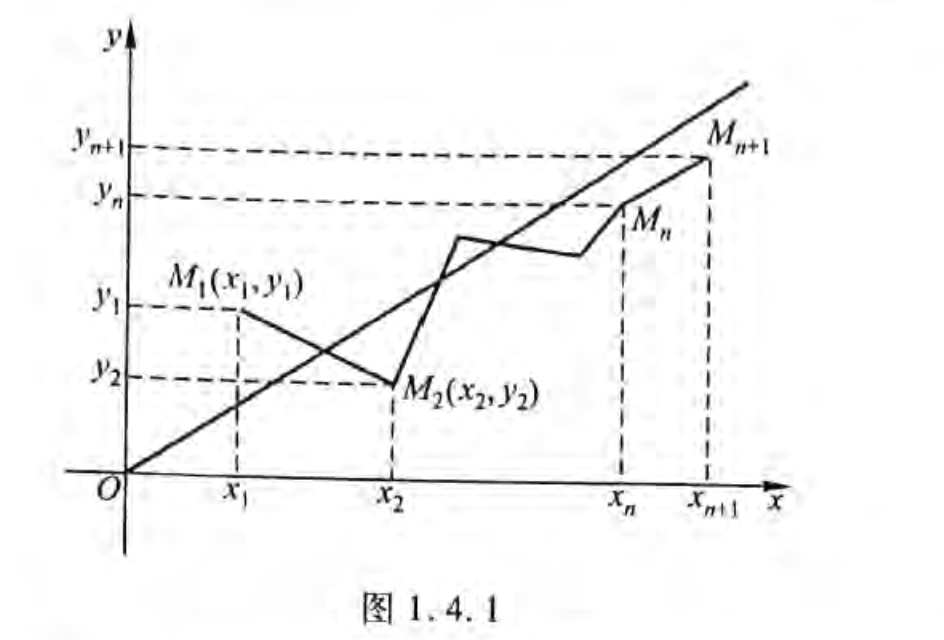
\includegraphics[width=0.45\textwidth]{1-4-1.png}
\end{figure}

\noindent\textbf{证}\quad
$1^\circ$ 已知
\[
  \lim_{n\to\infty}\frac{y_n-y_{n-1}}{x_n-x_{n-1}}=a,
\]
即 $\forall\varepsilon>0$，$\exists N>0$，当 $n>N$ 时，有
\[
  \left|\frac{y_n-y_{n-1}}{x_n-x_{n-1}}-a\right|<\frac\varepsilon2,
\]
即
\[
  a-\frac\varepsilon2
  <\frac{y_k-y_{k-1}}{x_k-x_{k-1}}
  <a+\frac\varepsilon2
  \quad(k=N+1,N+2,\cdots,n-1,n,\cdots). \tag{1}
\]
借助分数的和比性质：“当
$m<\dfrac{b_k}{a_k}<M\ (k=1,2,\cdots,n)$ 时，有
$m<\dfrac{b_1+b_2+\cdots+b_n}{a_1+a_2+\cdots+a_n}<M$”.
于是，由式 (1) 可得
\[
  a-\frac\varepsilon2
  <\frac{y_n-y_N}{x_n-x_N}
  <a+\frac\varepsilon2,
\]
亦即
\[
  \left|\frac{y_n-y_N}{x_n-x_N}-a\right|<\frac\varepsilon2. \tag{2}
\]
另一方面，
\[
\begin{aligned}
  \frac{y_n}{x_n}-a
  &=\frac{y_n-ax_n}{x_n}\\
  &=\frac{y_n-y_N-ax_n+ax_N}{x_n-x_N}\cdot
  \frac{x_n-x_N}{x_n}+\frac{y_N-ax_N}{x_n}\\
  &=\left(\frac{y_n-y_N}{x_n-x_N}-a\right)
  \left(1-\frac{x_N}{x_n}\right)+\frac{y_N-ax_N}{x_n}.
\end{aligned} \tag{3}
\]
因 $x_n$ 严格增加趋向 $+\infty$，可默认 $x_n>0$；当 $n>N$ 时，有
$\left|1-\dfrac{x_N}{x_n}\right|\le1$. 固定 $N$，让 $n$ 进一步增大，还能保持
\[
  \left|\frac{y_N-ax_N}{x_n}\right|<\frac\varepsilon2.
\]
故由式 (3) 得
\[
  \left|\frac{y_n}{x_n}-a\right|
  \le
  \left|\frac{y_n-y_N}{x_n-x_N}-a\right|
  +\left|\frac{y_N-ax_N}{x_n}\right|
  \stackrel{\text{式(2)}}{<}
  \frac\varepsilon2+\frac\varepsilon2=\varepsilon,
\]
亦即 $\displaystyle\lim_{n\to\infty}\frac{y_n}{x_n}=a$. 证毕.

$2^\circ$（极限为 $+\infty$ 的情况）因已知
\[
  \lim_{n\to\infty}\frac{y_n-y_{n-1}}{x_n-x_{n-1}}=+\infty,
\]
所以
\[
  \lim_{n\to\infty}\frac{x_n-x_{n-1}}{y_n-y_{n-1}}=0.
\]
利用 $1^\circ$ 中的结论，只要证明 $y_n$ 严格增加趋向 $+\infty$，则
\[
  \lim_{n\to\infty}\frac{x_n}{y_n}=0,\quad
  \lim_{n\to\infty}\frac{y_n}{x_n}=+\infty
\]
（问题得证）. 因 $x_n$ 严格递增，要证 $y_n$ 严格递增，只要证
\[
  \frac{y_n-y_{n-1}}{x_n-x_{n-1}}>1.
\]
事实上，
\[
  \lim_{n\to\infty}\frac{y_n-y_{n-1}}{x_n-x_{n-1}}=+\infty,
\]
所以对 $M=1$，$\exists N>0$，当 $n>N$ 时，有
\[
  \frac{y_n-y_{n-1}}{x_n-x_{n-1}}>1,
\]
即
\[
  y_n-y_{n-1}>x_n-x_{n-1}>0. \tag{4}
\]
所以当 $n>N$ 时，$y_n$ 严格递增. 在式 (4) 中令 $n=N+1,N+2,\cdots,k$，然后相加，可知
\[
  y_k-y_N>x_k-x_N.
\]
令 $k\to\infty$，知 $y_k\to+\infty$. 证毕.

$3^\circ$（极限为 $-\infty$ 的情况）只要令 $y_n=-z_n$，即可转化为 $2^\circ$ 中的情况.

\noindent\textbf{注}\quad
\[
  \lim_{n\to\infty}\frac{y_n-y_{n-1}}{x_n-x_{n-1}}=\infty
\]
一般推不出
\[
  \lim_{n\to\infty}\frac{y_n}{x_n}=\infty.
\]
如令 $x_n=n$，$|y_n|=\{0,2^2,0,4^2,0,6^2,\cdots\}$，这时虽然
\[
  \lim_{n\to\infty}\frac{y_n-y_{n-1}}{x_n-x_{n-1}}=\infty,
\]
但
\[
  \left\{\frac{y_n}{x_n}\right\}=\{0,2,0,4,0,6,\cdots\}\not\to\infty.
\]

\noindent\textbf{定理 2（$\dfrac00$ 型 Stolz 公式）}\quad
设 $n\to\infty$ 时 $y_n\to0$，$x_n$ 严格单调下降趋向零.
若
\[
  \lim_{n\to\infty}\frac{y_n-y_{n-1}}{x_n-x_{n-1}}=a,
\]
则
\[
  \lim_{n\to\infty}\frac{y_n}{x_n}=a
\]
（其中 $a$ 为有限数，$+\infty$ 或 $-\infty$）.

\noindent\textbf{注}\quad 由证明看出，定理 1 其名为 $\dfrac\infty\infty$ 型，其实只要求分母 $x_n\nearrow+\infty$（严格单调上升趋向无穷大），至于分子 $y_n$ 是否趋向无穷大，无关紧要. 定理 2 则是名副其实的 $\dfrac00$ 型，因为定理条件要求分子、分母都以 0 为极限.

Stolz 公式对于求序列的极限十分有用. 例 1.2.1 中 2），如果应用 Stolz 公式，变得非常明显. 因 $\displaystyle\lim_{n\to\infty}x_n=A$，所以
\[
  \lim_{n\to\infty}\frac{x_1+x_2+\cdots+x_n}{n}
  =\lim_{n\to\infty}\frac{x_n}{1}=A.
\]
又如

\noindent\textbf{例 1.4.1}\quad 证明：
\[
  \lim_{n\to\infty}\frac{1^p+2^p+\cdots+n^p}{n^{p+1}}
  =\frac1{p+1}
\]
（$p$ 为自然数）.

\noindent\textbf{证}\quad
\[
\begin{aligned}
  \lim_{n\to\infty}\frac{1^p+2^p+\cdots+n^p}{n^{p+1}}
  &=\lim_{n\to\infty}\frac{(n+1)^p}{(n+1)^{p+1}-n^{p+1}}\\
  &=\lim_{n\to\infty}
  \frac{(1+n)^p}{(p+1)n^p+\dfrac{(p+1)p}{2}n^{p-1}+\cdots+1}\\
  &=\frac1{p+1}.
\end{aligned}
\]

Stolz 公式必要时可以重复使用.

\noindent\textbf{例 1.4.2}\quad 设
\[
  S_n=\frac{\displaystyle\sum_{k=0}^n\ln C_n^k}{n^2}
  \quad\left(\text{其中 }C_n^k=\frac{n(n-1)\cdots(n-k+1)}{1\cdot2\cdots k}\right),
\]
求 $\displaystyle\lim_{n\to\infty}S_n$.

\noindent\textbf{解}\quad 因 $n^2\nearrow+\infty$，应用 Stolz 公式，
\[
\begin{aligned}
  \lim_{n\to\infty}S_n
  &=\lim_{n\to\infty}
  \frac{\displaystyle\sum_{k=0}^{n+1}\ln C_{n+1}^k-\sum_{k=1}^n\ln C_n^k}{(n+1)^2-n^2}\\
  &=\lim_{n\to\infty}
  \frac{\displaystyle\sum_{k=0}^n\ln\frac{C_{n+1}^k}{C_n^k}+\ln C_{n+1}^{n+1}}{2n+1}\\
  &=\lim_{n\to\infty}
  \frac{\displaystyle\sum_{k=0}^n\ln\frac{n+1}{n-k+1}}{2n+1}\\
  &=\lim_{n\to\infty}
  \frac{(n+1)\ln(n+1)-\displaystyle\sum_{k=1}^{n+1}\ln k}{2n+1}
  \quad(\text{再次使用 Stolz 公式})\\
  &=\lim_{n\to\infty}
  \frac{(n+1)\ln(n+1)-n\ln n-\ln(n+1)}
  {(2n+1)-(2n-1)}\\
  &=\lim_{n\to\infty}
  \frac{\ln\left(\dfrac{n+1}{n}\right)^n}{2}
  =\frac12.
\end{aligned}
\]
有时问题经过处理之后，方能应用 Stolz 公式.

\noindent\textbf{例 1.4.3}\quad 设
\[
  \lim_{n\to\infty}n(A_n-A_{n-1})=0.
\]
试证：极限
\[
  \lim_{n\to\infty}\frac{A_1+A_2+\cdots+A_n}{n}
\]
存在时，
\[
  \lim_{n\to\infty}A_n
  =\lim_{n\to\infty}\frac{A_1+A_2+\cdots+A_n}{n}.
\]

\noindent\textbf{证}\quad 因
\[
  A_n=\left(A_n-\frac{A_1+\cdots+A_n}{n}\right)+
  \frac{A_1+\cdots+A_n}{n},
\]
只需证明第一项趋于零. 为了利用 $\displaystyle\lim_{n\to\infty}n(A_n-A_{n-1})=0$，特令
\[
  a_1=A_1,\quad a_2=A_2-A_1,\quad\cdots,\quad
  a_n=A_n-A_{n-1},\quad\cdots,
\]
则知 $\displaystyle\lim_{n\to\infty}na_n=0$，且
\[
  A_n=(A_n-A_{n-1})+(A_{n-1}-A_{n-2})+\cdots+(A_2-A_1)+A_1
  =a_n+a_{n-1}+\cdots+a_1.
\]
于是
\[
\begin{aligned}
  \lim_{n\to\infty}\left(A_n-\frac{A_1+\cdots+A_n}{n}\right)
  &=\lim_{n\to\infty}\left[(a_1+\cdots+a_n)-
  \frac{a_1+(a_1+a_2)+\cdots+(a_1+\cdots+a_n)}n\right]\\
  &=\lim_{n\to\infty}\frac{a_2+2a_3+\cdots+(n-1)a_n}{n}
  \quad(\text{应用 Stolz 公式})\\
  &=\lim_{n\to\infty}\frac{(n-1)a_n}{n-(n-1)}
  =\lim_{n\to\infty}\frac{n-1}{n}\cdot na_n=0.
\end{aligned}
\]

\noindent\textbf{例 1.4.4}\quad 求
\[
  \lim_{n\to\infty}
  \left(\frac2{2^2-1}\right)^{\frac1{2^{n-1}}}
  \left(\frac{2^2}{2^3-1}\right)^{\frac1{2^{n-2}}}
  \cdots
  \left(\frac{2^{n-1}}{2^n-1}\right)^{\frac12}.
\]

\noindent\textbf{解}\quad 先取对数，再求极限.
\[
\begin{aligned}
  \ln x_n
  &=\frac1{2^{n-1}}\ln\frac2{2^2-1}
  +\frac1{2^{n-2}}\ln\frac{2^2}{2^3-1}
  +\cdots+\frac12\ln\frac{2^{n-1}}{2^n-1}\\
  &=\frac1{2^{n-1}}\left(\ln\frac2{2^2-1}
  +2\ln\frac{2^2}{2^3-1}
  +\cdots+2^{n-2}\ln\frac{2^{n-1}}{2^n-1}\right).
\end{aligned}
\]
应用 Stolz 公式，
\[
  \lim_{n\to\infty}\ln x_n
  =\lim_{n\to\infty}
  \frac{2^{n-2}\ln\dfrac{2^{n-1}}{2^n-1}}{2^{n-1}-2^{n-2}}
  =\lim_{n\to\infty}\ln\frac1{2-\dfrac1{2^{n-1}}}
  =\ln\frac12.
\]
故
\[
  \text{原式}=\lim_{n\to\infty}x_n=\frac12.
\]

\subsection*{二、函数极限的情况}

Stolz 公式可以推广到函数极限的情况.

\noindent\textbf{定理 $1'$（$\dfrac\infty\infty$ 型）}\quad 若 $T>0$ 为常数，

1）$g(x+T)>g(x),\ \forall x\ge a$；

2）$g(x)\to+\infty$（当 $x\to+\infty$ 时），且 $f,g$ 在 $[a,+\infty)$ 内闭有界（即指 $\forall b>a$，$f,g$ 在 $[a,b]$ 上有界）；

3）
\[
  \lim_{x\to+\infty}\frac{f(x+T)-f(x)}{g(x+T)-g(x)}=l,
\]
则
\[
  \lim_{x\to+\infty}\frac{f(x)}{g(x)}=l
\]
（其中 $l$ 为有限数，或 $+\infty$，或 $-\infty$）.

\noindent\textbf{证}\quad
$1^\circ$（$l$ 为有限数）要证明
\[
  \lim_{x\to+\infty}\frac{f(x)}{g(x)}=l,
\]
即要证明 $\forall\varepsilon>0$，$\exists\Delta>0$，当 $x>\Delta$ 时，有
\[
  \left|\frac{f(x)}{g(x)}-l\right|<\varepsilon. \tag{1}
\]
由已知条件 $g(x)\to+\infty$ 及
\[
  \lim_{x\to+\infty}\frac{f(x+T)-f(x)}{g(x+T)-g(x)}=l
\]
知，$\forall\varepsilon>0$，$\exists A>0$，当 $x>A$ 时，有 $g(x)>0$，
\[
  \left|\frac{f(x+T)-f(x)}{g(x+T)-g(x)}-l\right|<\frac\varepsilon2. \tag{2}
\]
至此，我们若能证明 $\forall\varepsilon>0$，$\exists N>0$，当 $n>N$ 时，对任意
$x\in[A,A+T]$，恒有
\[
  \left|\frac{f(x+nT)}{g(x+nT)}-l\right|<\varepsilon, \tag{3}
\]
则式 (1) 获证. 事实上，$\forall y>A+NT$，总 $\exists n>N$ 及
$x\in[A,A+T]$，使得
\[
  y=x+nT.
\]
从而由式 (3) 知 $\forall y>A+NT$，有
\[
  \left|\frac{f(y)}{g(y)}-l\right|<\varepsilon.
\]
这表明式 (1) 成立.

剩下的问题在于从式 (2) 推证式 (3). 我们采用本节定理 1 类似的方法.

记
\[
  \alpha_n=
  \frac{f(x+nT)-f(x+(n-1)T)}
  {g(x+nT)-g(x+(n-1)T)}-l. \tag{4}
\]
则
\[
\begin{aligned}
f(x+nT)
&=f(x+(n-1)T)+[g(x+nT)-g(x+(n-1)T)](\alpha_n+l)\\
&=f(x+(n-2)T)+[g(x+(n-1)T)-g(x+(n-2)T)](\alpha_{n-1}+l)\\
&\quad+[g(x+nT)-g(x+(n-1)T)](\alpha_n+l)\\
&=\cdots\\
&=f(x+T)+[g(x+2T)-g(x+T)](\alpha_2+l)+\cdots\\
&\quad+[g(x+nT)-g(x+(n-1)T)](\alpha_n+l)\\
&=f(x+T)+\alpha_2[g(x+2T)-g(x+T)]+\cdots\\
&\quad+\alpha_n[g(x+nT)-g(x+(n-1)T)]
  +l[g(x+nT)-g(x+T)].
\end{aligned}
\]
再除以 $g(x+nT)$，减去 $l$，得
\[
\begin{aligned}
\left|\frac{f(x+nT)}{g(x+nT)}-l\right|
&\le
\left|\frac{f(x+T)-lg(x+T)}{g(x+nT)}\right|\\
&\quad+\frac1{|g(x+nT)|}\bigl[
|\alpha_2|\,|g(x+2T)-g(x+T)|+\cdots\\
&\qquad\qquad\qquad
 +|\alpha_n|\,|g(x+nT)-g(x+(n-1)T)|\bigr].
\end{aligned}
\]
由式 (2) 知 $|\alpha_k|<\dfrac\varepsilon2\ (k=1,2,\cdots,n)$，注意定理条件 1），上式右端
\[
\le
\left|\frac{f(x+T)-lg(x+T)}{g(x+nT)}\right|
+\frac\varepsilon2
\left|\frac{g(x+nT)-g(x+T)}{g(x+nT)}\right|
\le
\left|\frac{f(x+T)-lg(x+T)}{g(x+nT)}\right|+\frac\varepsilon2.
\]
按条件，$f(x+T)-lg(x+T)$ 在 $[A,A+T]$ 上有界，即 $\exists M>0$，使得
$|f(x+T)-lg(x+T)|\le M$. 于是
\[
  \text{上式右端}\le\frac{M}{|g(x+nT)|}+\frac\varepsilon2.
\]
但 $g(x)\to+\infty\ (x\to+\infty)$，故 $\exists N>0$，当 $n>N$ 时有
\[
  \frac{M}{|g(x+nT)|}<\frac\varepsilon2,
\]
所以
\[
  \left|\frac{f(x+nT)}{g(x+nT)}-l\right|
  <\frac\varepsilon2+\frac\varepsilon2=\varepsilon.
\]

$2^\circ$ 因
\[
  \lim_{x\to+\infty}g(x)=+\infty,\quad
  \lim_{x\to+\infty}\frac{f(x+T)-f(x)}{g(x+T)-g(x)}=+\infty,
\]
故 $\forall M>0$，$\exists A>a$，当 $x>A$ 时，$g(x)>0$，
\[
  \frac{f(x+T)-f(x)}{g(x+T)-g(x)}>2M.
\]
从而 $\forall n\in\mathbb N$，有
\[
  \frac{f(x+nT)-f(x+(n-1)T)}
  {g(x+nT)-g(x+(n-1)T)}>2M.
\]
由此
\[
\begin{aligned}
f(x+nT)
&>f(x+(n-1)T)+2M[g(x+nT)-g(x+(n-1)T)]\\
&>f(x+(n-2)T)+2M[g(x+(n-1)T)-g(x+(n-2)T)]\\
&\quad+2M[g(x+nT)-g(x+(n-1)T)]\\
&>\cdots\\
&>f(x)+2M[g(x+T)-g(x)]+\cdots
  +2M[g(x+nT)-g(x+(n-1)T)]\\
&=f(x)+2M[g(x+nT)-g(x)].
\end{aligned}
\]
两边同时除以 $g(x+nT)$，
\[
  \frac{f(x+nT)}{g(x+nT)}
  >2M+\frac{f(x)-2Mg(x)}{g(x+nT)}.
\]
注意到 $f(x)-2Mg(x)$ 在 $[A,A+T]$ 上有界，而 $g(x+nT)\to+\infty$，所以
$\exists N>0$，$n\ge N$ 时，
\[
  \frac{f(x)-2Mg(x)}{g(x+nT)}>-M,
\]
于是
\[
  \frac{f(x+nT)}{g(x+nT)}>2M-M=M.
\]
因 $\forall y>A+NT$，$\exists n\ge N$ 及 $x\in[A,A+T]$，使得 $y=x+nT$. 故
\[
  \frac{f(y)}{g(y)}=\frac{f(x+nT)}{g(x+nT)}>M.
\]
此即表明
\[
  \lim_{x\to+\infty}\frac{f(x)}{g(x)}=+\infty.
\]

$3^\circ$ $l=-\infty$ 的情况，可考虑 $-f(x)$ 化为 $2^\circ$ 的情况.

对 $\dfrac00$ 型的 Stolz 公式，有类似的推广.

\noindent\textbf{定理 $2'$（$\dfrac00$ 型）}\quad 设 $T>0$，且

1）$0<g(x+T)<g(x)\ (\forall x\ge a)$；

2）$\displaystyle\lim_{x\to+\infty}f(x)=\lim_{x\to+\infty}g(x)=0$；

3）$\displaystyle\lim_{x\to+\infty}\frac{f(x+T)-f(x)}{g(x+T)-g(x)}=l$；

则
\[
  \lim_{x\to+\infty}\frac{f(x)}{g(x)}=l
\]
（其中 $l$ 为有限数，或 $+\infty$，或 $-\infty$）.

有些问题，用上述定理可变得十分容易. 如

\noindent\textbf{*例 1.4.5（Cauchy 定理）}\quad
若 $f$ 在 $(a,+\infty)$ 内有定义，且内闭有界（即 $\forall[\alpha,\beta]\subset(a,+\infty)$，$f$ 在 $[\alpha,\beta]$ 上有界），则

1）
\[
  \lim_{x\to+\infty}\frac{f(x)}x
  =\lim_{x\to+\infty}[f(x+1)-f(x)];
\]
2）
\[
  \lim_{x\to+\infty}[f(x)]^{1/x}
  =\lim_{x\to+\infty}\frac{f(x+1)}{f(x)}
  \quad(f(x)\ge c>0),
\]
当右边极限存在时成立.

\noindent\textbf{*例 1.4.6}\quad
设 $f$ 在 $[a,+\infty)$ 上定义，且内闭有界，
\[
  \lim_{x\to+\infty}\frac{f(x+1)-f(x)}{x^n}=l
\]
（$l=$ 有限数，$+\infty$，$-\infty$），证明：
\[
  \lim_{x\to+\infty}\frac{f(x)}{x^{n+1}}=\frac{l}{n+1}.
\]

\noindent\textbf{证}\quad
\[
\begin{aligned}
  \lim_{x\to+\infty}\frac{f(x)}{x^{n+1}}
  &=\lim_{x\to+\infty}
  \frac{f(x+1)-f(x)}{(x+1)^{n+1}-x^{n+1}}\\
  &=\lim_{x\to+\infty}
  \frac{f(x+1)-f(x)}
  {(n+1)x^n+\dfrac{(n+1)n}{1\cdot2}x^{n-1}+\cdots+1}\\
  &=\lim_{x\to+\infty}
  \frac{\dfrac{f(x+1)-f(x)}{x^n}}
  {(n+1)+\dfrac{(n+1)n}{1\cdot2}\dfrac1x+\cdots+\dfrac1{x^n}}\\
  &=\frac{l}{n+1}.
\end{aligned}
\]
（$l$ 为 $+\infty,-\infty$ 也成立.）

\subsection*{单元练习 1.4}

\noindent\textbf{$\star$1.4.1}\quad 求 $\displaystyle\lim_{n\to\infty}x_n$，其中

1）$x_n=\sqrt[n]{n}$；\quad $\langle1\rangle$

2）$\displaystyle x_n=\frac1{\sqrt[n]{n!}}$；\quad $\langle0\rangle$

\noindent\textbf{提示}\quad 取对数后再用 Stolz 公式.

\noindent\textbf{$\star$1.4.2}\quad 求
\[
  \lim_{n\to\infty}\frac{1+\sqrt2+\sqrt[3]3+\cdots+\sqrt[n]n}{n}.
\]
（华中师范大学）\quad $\langle1\rangle$

\noindent\textbf{1.4.3}\quad 已知数列 $\{x_n\}$ 满足条件
\[
  \lim_{n\to\infty}(x_n-x_{n-2})=0,
\]
证明：
\[
  \lim_{n\to\infty}\frac{x_n-x_{n-1}}n=0.
\]
（四川大学）

\noindent\textbf{证 I}\quad 应用 Stolz 公式（当分母单调增加趋向 $+\infty$ 时，无须检验分子是否趋向 $+\infty$），
\[
  \lim_{n\to\infty}\frac{x_n-x_{n-1}}n
  \overset{\text{Stolz 公式}}{=}
  \lim_{n\to\infty}\frac{(x_n-x_{n-1})-(x_{n-1}-x_{n-2})}{n-(n-1)}
  =0.
\]

\noindent\textbf{证 II}\quad 见例 1.2.3.

\noindent\textbf{证 III}\quad 因
\[
  \lim_{n\to\infty}(x_n-x_{n-2})=0,
\]
故 $\forall\varepsilon>0$，$\exists N>0$，$\forall n\ge N+2$，有
$|x_n-x_{n-2}|<\dfrac\varepsilon2$. 于是
\[
  |x_{2k}-x_{2(k-1)}|<\frac\varepsilon2
  \quad(\forall k=N+1,N+2,\cdots),
\]
\[
  |x_{2k}-x_{2N}|
  =\left|\sum_{i=N+1}^k(x_{2i}-x_{2(i-1)})\right|
  \le\sum_{i=N+1}^k|x_{2i}-x_{2(i-1)}|
  <(k-N)\frac\varepsilon2.
\]
注意此时 $N$ 已被固定，可取更大的 $K>N$，使得 $k>K$ 时，有
$\dfrac{|x_{2N}|}{2k}<\dfrac\varepsilon2$. 于是当 $k>K$ 时，有
\[
  \frac{|x_{2k}|}{2k}
  \le\frac{|x_{2k}-x_{2N}|+|x_{2N}|}{2k}
  \le\frac\varepsilon2+\frac\varepsilon2=\varepsilon.
\]
至此证明了：
\[
  \lim_{k\to\infty}\frac{|x_{2k}|}{2k}=0.
\]
类似可证：极限
\[
  \lim_{k\to\infty}\frac{|x_{2k+1}|}{2k+1}=0.
\]
利用例 1.2.13 的结论，知
\[
  \lim_{n\to\infty}\frac{|x_n|}{n}=0.
\]
最后得
\[
  \lim_{n\to\infty}\frac{x_n-x_{n-1}}n
  =\lim_{n\to\infty}\left(\frac{x_n}{n}-\frac{n-1}{n}\cdot\frac{x_{n-1}}{n-1}\right)=0.
\]
问题获证.

\noindent\textbf{$\star$1.4.4}\quad 设 $\displaystyle\lim_{n\to\infty}x_n=a$.

1）若 $a$ 为有限数，证明：
\[
  \lim_{n\to\infty}\frac{x_1+2x_2+\cdots+nx_n}{n(n+1)}=\frac a2;
\]

2）若 $a$ 为 $+\infty$，证明：
\[
  \frac{x_1+2x_2+\cdots+nx_n}{n(n+1)}=+\infty.
\]
（南京大学）

\noindent\textbf{$\star$1.4.5}\quad 证明：若数列 $\{a_n\}$ 收敛于 $a$，且
$\displaystyle\lim_{n\to\infty}\sum_{k=1}^n p_k=+\infty$，$p_k\ge0\ (k=1,2,\cdots)$，则
\[
  \lim_{n\to\infty}
  \frac{\displaystyle\sum_{k=1}^n p_ka_k}
  {\displaystyle\sum_{k=1}^n p_k}=a.
\]
（东北师范大学）

\noindent\textbf{*1.4.6}\quad 已知 $\displaystyle\lim_{n\to\infty}\sum_{k=1}^n a_k$ 存在，
$\{p_n\}$ 为单调增加的正数列，且 $\displaystyle\lim_{n\to\infty}p_n=+\infty$，
$p_{n+1}\ne p_n\ (n=1,2,\cdots)$，求证：
\[
  \lim_{n\to\infty}\frac{p_1a_1+p_2a_2+\cdots+p_na_n}{p_n}=0.
\]
（北京师范大学）

\noindent\textbf{提示}\quad 记 $S_n=\sum_{k=1}^n a_k$，则
\[
  \sum_{k=1}^np_ka_k
  =\sum_{k=2}^np_k(S_k-S_{k-1})+p_1S_1
  =\sum_{k=1}^{n-1}S_k(p_k-p_{k+1})+S_np_n,
\]

\noindent\textbf{再提示}\quad
\[
  \lim_{n\to\infty}
  \frac{\displaystyle\sum_{k=1}^{n-1}S_k(p_k-p_{k+1})}{p_n}
  =\lim_{n\to\infty}(-S_{n-1}).
\]

\noindent\textbf{*1.4.7}\quad 若 $0<\lambda<1$，$a_n>0$，且
\[
  \lim_{n\to\infty}a_n=a,
\]
试证
\[
  \lim_{n\to\infty}(a_n+\lambda a_{n-1}+\lambda^2a_{n-2}+\cdots+\lambda^na_0)
  =\frac{a}{1-\lambda}.
\]

\noindent\textbf{提示}\quad 令 $a_k=a+\alpha_k$，再用 $\dfrac\infty\infty$ 型 Stolz 公式.

\noindent\textbf{再提示}\quad
\[
  \lim_{n\to\infty}\sum_{k=0}^n\lambda^ka_{n-k}
  =\lim_{n\to\infty}\sum_{i=0}^n\lambda^{n-i}a_i
  =\lim_{n\to\infty}
  \frac{\displaystyle\sum_{i=0}^n\lambda^{-i}a_i}{\lambda^{-n}}.
\]

\noindent\textbf{*1.4.8}\quad 求极限

1）
\[
  \lim_{n\to\infty}\frac{1^k+2^k+\cdots+n^k}{n^{k+1}};
\]
\quad $\left\langle\frac1{k+1}\right\rangle$

2）
\[
  \lim_{n\to\infty}\left(\frac{1^k+2^k+\cdots+n^k}{n^k}-\frac n{k+1}\right).
\]
\quad $\left\langle\frac12\right\rangle$

\noindent\textbf{提示}\quad 2）通分之后再用 Stolz 公式.

\noindent\textbf{**1.4.9}\quad 设
\[
  \lim_{n\to\infty}\sum_{k=1}^n\frac1{k^2}=m,
\]
求极限
\[
  \lim_{n\to\infty}n^2\left(m-\sum_{k=1}^n\frac1{k^2}-\frac1n\right).
\]
\quad $\left\langle-\frac12\right\rangle$

\noindent\textbf{提示}\quad 用 $\dfrac00$ 型 Stolz 公式：
\[
  \text{原极限}
  =\lim_{n\to\infty}
  \frac{-\dfrac1{n^2}+\dfrac1{n(n-1)}}{\dfrac{-2n+1}{n^2(n-1)^2}}
  =-\frac12.
\]

\noindent\textbf{注}\quad 这里 $\displaystyle m=\lim_{n\to\infty}\sum_{k=1}^n\frac1{k^2}=\frac{\pi^2}{6}$（见例 5.4.11）.

请思考一下：条件“$\displaystyle\lim_{n\to\infty}\sum_{k=1}^n\frac1{k^2}=m$”用在何处？

\section*{§1.5\quad 递推形式的极限}

有些数列，常常是利用递推的形式给出. 如何计算这类数列的极限，是本节的中心问题.

\subsection*{一、利用存在性求极限}

\noindent\textbf{要点}\quad 假若用某种方法证明了递推数列的极限存在，则在递推公式里取极限，便可得极限值 $A$ 应满足的方程. 解此方程，可求极限值 $A$.

证明数列的极限存在，常采用两种方法：

1）利用单调有界原理.

若 $x_n\nearrow$ 有上界，或 $x_n\searrow$ 有下界，则 $\{x_n\}$ 收敛.

判断单调性，通常方法是
\[
  \text{(1) }\forall n\in\mathbb N:\ x_{n+1}-x_n
  \begin{cases}
    \ge0,\text{ 则 }x_n\nearrow,\\
    \le0,\text{ 则 }x_n\searrow,
  \end{cases}
\]
\[
  \text{(2) }\forall n\in\mathbb N:\ \frac{x_{n+1}}{x_n}
  \begin{cases}
    \ge1,\text{ 则 }x_n\nearrow,\\
    \le1,\text{ 则 }x_n\searrow.
  \end{cases}
\]
\[
  \text{(3) 若 }x_{n+1}=f(x_n),\ f'(x)\ge0,\text{ 则}
\]
当 $x_1\le x_2$ 时，$x_n\nearrow$；当 $x_1\ge x_2$ 时，$x_n\searrow$
（这是根据 $x_{n+1}-x_n=f(x_n)-f(x_{n-1})=f'(\xi_n)(x_n-x_{n-1})$，利用数学归纳法得到的）.

此外，数学归纳法以及常用的不等式都是证明单调、有界的重要工具.

2）利用“压缩映像”原理.

\noindent\textbf{定理}\quad $1^\circ$ 对于任一数列 $\{x_n\}$ 而言，若存在常数 $r$，使得 $\forall n\in\mathbb N$，恒有
\[
  |x_{n+1}-x_n|\le r|x_n-x_{n-1}|,\quad 0<r<1, \tag{A}
\]
则数列 $\{x_n\}$ 收敛.

$2^\circ$\quad 特别，若数列 $\{x_n\}$ 利用递推公式给出：
\[
  x_{n+1}=f(x_n), \quad n=1,2,\cdots,
\]
其中 $f$ 为某一可微函数，且 $\exists r\in\mathbb R$，使得
\[
  |f'(x)|\le r<1\quad (\forall x\in\mathbb R), \tag{B}
\]
则数列 $\{x_n\}$ 收敛.

\noindent\textbf{证}\quad $1^\circ$ 由式 (A) 知：
\[
  |x_{n+1}-x_n|\le r|x_n-x_{n-1}|\le \cdots\le r^{n-1}|x_2-x_1|.
\]
若 $m>n$，则
\[
\begin{aligned}
  |x_m-x_n|
  &\le |x_m-x_{m-1}|+\cdots+|x_{n+1}-x_n|\\
  &\le (r^{m-2}+\cdots+r^{n-1})|x_2-x_1|
  < \frac{r^{n-1}}{1-r}|x_2-x_1|.
\end{aligned}
\]
由于 $0<r<1$，故 $\lim\limits_{n\to\infty}r^{n-1}=0$. 因而 $\{x_n\}$ 满足 Cauchy 准则，故 $\{x_n\}$ 收敛.

$2^\circ$ 若式 (B) 成立，由微分中值定理得
\[
  |x_{n+1}-x_n|=|f(x_n)-f(x_{n-1})|
  \le r|x_n-x_{n-1}|,
\]
由 $1^\circ$ 知 $\{x_n\}$ 收敛.

\noindent\textbf{注}\quad 若式 (B) 只在某区间 $I$ 上成立，只要数列 $\{x_n\}$ 取值于 $I$，上述结论仍成立.

\noindent\textbf{$\star$例 1.5.1}\quad 设 $a>0$，数列 $\{x_n\}$ 由
\[
  x_1=a,\qquad x_{n+1}=\frac{1}{2}\left(x_n+\frac{a}{x_n}\right),\quad n=1,2,\cdots
\]
给出，求证 $\lim\limits_{n\to\infty}x_n=\sqrt a$.

\noindent\textbf{证 I}\quad 先证单调有界. 由于 $x_1=a>0$，由递推式知 $x_n>0$，且
\[
  x_{n+1}-\sqrt a
  =\frac{x_n^2+a-2\sqrt a\,x_n}{2x_n}
  =\frac{(x_n-\sqrt a)^2}{2x_n}\ge 0,
\]
故 $x_{n+1}\ge \sqrt a$. 又
\[
  x_{n+1}-x_n
  =\frac{a-x_n^2}{2x_n}
  \le 0\quad (n\ge 2),
\]
故 $\{x_n\}_{n=2}^\infty$ 单调下降且有下界 $\sqrt a$，因而收敛. 设其极限为 $A$，令 $n\to\infty$ 于递推式中，得
\[
  A=\frac{1}{2}\left(A+\frac{a}{A}\right),
\]
从而 $A=\sqrt a$.

\noindent\textbf{证 II}\quad 先证 $\{x_n\}$ 为 Cauchy 列. 由
\[
  x_{n+1}-\sqrt a=\frac{(x_n-\sqrt a)^2}{2x_n}
\]
及 $x_n\ge \sqrt a\ (n\ge 2)$，有
\[
  |x_{n+1}-\sqrt a|\le \frac{1}{2\sqrt a}|x_n-\sqrt a|^2.
\]
这说明误差迅速缩小，从而 $\{x_n\}$ 收敛，代入递推式仍得极限为 $\sqrt a$.

\noindent\textbf{证 III}\quad 令 $y_n=x_n/\sqrt a$，则
\[
  y_{n+1}=\frac{1}{2}\left(y_n+\frac{1}{y_n}\right).
\]
由于
\[
  y_{n+1}-1=\frac{(y_n-1)^2}{2y_n},\qquad
  y_{n+1}-y_n=\frac{1-y_n^2}{2y_n},
\]
同证 I 可知 $y_n\to 1$，于是 $x_n\to \sqrt a$.

\noindent\textbf{证 IV}\quad 记
\[
  f(x)=\frac{1}{2}\left(x+\frac{a}{x}\right).
\]
在区间 $[\sqrt a,+\infty)$ 上，
\[
  |f'(x)|=\frac{1}{2}\left|1-\frac{a}{x^2}\right|\le \frac12.
\]
又由递推式知 $x_n\in[\sqrt a,+\infty)$（$n\ge2$），故由压缩映像定理知 $\{x_n\}$ 收敛. 设极限为 $A$，则 $A=f(A)$，因而 $A=\sqrt a$.

\noindent\textbf{练习 1}\quad 已知
\[
  0<x_1<1,\qquad x_{n+1}=\sqrt{1-x_n},\quad n=1,2,\cdots.
\]
求证 $\{x_n\}$ 收敛，并求其极限.

\noindent\textbf{提示}\quad 设 $f(x)=\sqrt{1-x}$，则 $f$ 在 $[0,1]$ 上将 $[0,1]$ 映入自身，且
\[
  |f'(x)|=\frac{1}{2\sqrt{1-x}}.
\]
在包含所有 $x_n$ 的适当闭区间上可取到小于 $1$ 的 Lipschitz 常数，故由压缩映像定理知 $\{x_n\}$ 收敛. 设极限为 $A$，则
\[
  A=\sqrt{1-A},
\]
故
\[
  A=\frac{\sqrt5-1}{2}.
\]

\noindent\textbf{练习 2}\quad 设
\[
  0<x_1<\frac{\pi}{2},\qquad x_{n+1}=\sin x_n.
\]
证明 $\{x_n\}$ 收敛，并求极限.

\noindent\textbf{证}\quad 因为 $0<x<\frac{\pi}{2}$ 时 $\sin x<x$，故
\[
  0<x_{n+1}<x_n<\frac{\pi}{2}.
\]
所以 $\{x_n\}$ 单调下降且有下界 $0$，从而收敛. 设极限为 $A$，则
\[
  A=\sin A,
\]
故 $A=0$.

\noindent\textbf{练习 3}\quad 已知
\[
  x_1>0,\qquad x_{n+1}=\frac{1}{2}\left(x_n+\frac{2}{x_n}\right).
\]
求证 $\{x_n\}$ 收敛，并求其极限.

\noindent\textbf{$\star$例 1.5.2}\quad 设 $0<a<1$，
\[
  x_1>0,\qquad x_{n+1}=a+\frac{1}{x_n},\quad n=1,2,\cdots.
\]
求证 $\{x_n\}$ 收敛，并求其极限.

\noindent\textbf{提示}\quad 先证所有项均落在某个闭区间 $I=[\alpha,\beta]\subset(0,+\infty)$ 内，再考察
\[
  f(x)=a+\frac{1}{x},\qquad |f'(x)|=\frac{1}{x^2}.
\]
取适当的二次迭代或在不变区间上应用压缩映像思想，可得 $\{x_n\}$ 收敛. 极限 $A$ 满足
\[
  A=a+\frac{1}{A},
\]
因而
\[
  A=\frac{a+\sqrt{a^2+4}}{2}.
\]

\noindent\textbf{$\star$例 1.5.3（不动点方法）}\quad 设 $0<a<1$，
\[
  x_1>0,\qquad x_{n+1}=a+\frac{1}{x_n},\quad n=1,2,\cdots.
\]
求证 $\{x_n\}$ 收敛，并求其极限.

\noindent\textbf{证}\quad 设
\[
  f(x)=a+\frac1x,\qquad
  \alpha=\frac{a+\sqrt{a^2+4}}2.
\]
则 $\alpha=f(\alpha)$，即
\[
  \alpha=a+\frac1\alpha.
\]
由递推式得
\[
  x_{n+1}-\alpha
  =\frac{1}{x_n}-\frac{1}{\alpha}
  =-\frac{x_n-\alpha}{\alpha x_n}.
\]
从而
\[
  |x_{n+1}-\alpha|=\frac{|x_n-\alpha|}{\alpha x_n}.
\]
利用递推关系可知 $x_n$ 始终有正下界；并且当 $n$ 足够大时，$\alpha x_n$ 大于某个大于 $1$ 的常数，故误差按比例缩小，因而 $x_n\to\alpha$.

\noindent\textbf{练习}\quad 设
\[
  x_1>0,\qquad x_{n+1}=c\,\frac{1+x_n}{c+x_n}\quad (c>1),
\]
证明 $\{x_n\}$ 收敛，并求极限.

\noindent\textbf{解 I}\quad 设极限为 $A$，则
\[
  A=c\,\frac{1+A}{c+A},
\]
即
\[
  A^2=c.
\]
故可能的极限为 $\sqrt c$. 再由递推式可知 $x_n>0$，且
\[
  x_{n+1}-\sqrt c
  =c\,\frac{1+x_n}{c+x_n}-\sqrt c
  =\frac{(c-\sqrt c)(x_n-\sqrt c)}{c+x_n}.
\]
于是
\[
  |x_{n+1}-\sqrt c|
  =\frac{c-\sqrt c}{c+x_n}|x_n-\sqrt c|
  \le \frac{c-\sqrt c}{c}|x_n-\sqrt c|
  =\left(1-\frac1{\sqrt c}\right)|x_n-\sqrt c|.
\]
由于 $0<1-\frac1{\sqrt c}<1$，故 $x_n\to\sqrt c$.

\noindent\textbf{解 II}\quad 也可直接考察不动点函数
\[
  f(x)=c\,\frac{1+x}{c+x}.
\]
在 $(0,+\infty)$ 上，
\[
  f'(x)=\frac{c(c-1)}{(c+x)^2},
\]
故
\[
  0<f'(x)\le \frac{c-1}{c}<1.
\]
由压缩映像定理，$\{x_n\}$ 收敛，极限为 $\sqrt c$.

\noindent\textbf{解 III}\quad 由
\[
  \frac{x_{n+1}-\sqrt c}{x_{n+1}+\sqrt c}
  =\frac{c-\sqrt c}{c+\sqrt c}\,
   \frac{x_n-\sqrt c}{x_n+\sqrt c}
\]
得
\[
  \left|\frac{x_{n+1}-\sqrt c}{x_{n+1}+\sqrt c}\right|
  =\frac{\sqrt c-1}{\sqrt c+1}
   \left|\frac{x_n-\sqrt c}{x_n+\sqrt c}\right|.
\]
反复迭代即可推出 $x_n\to\sqrt c$.

\noindent\textbf{注}\quad 以上三种方法的共同点，是先找到递推函数的不动点，再证明迭代向该不动点靠近.

\noindent\textbf{*例 1.5.4}\quad 设
\[
  x_1=1,\quad x_2=\frac12,\quad
  x_{n+1}=\frac{1}{1+x_n}\quad (n=1,2,\cdots).
\]
证明 $\{x_n\}$ 收敛，并求其极限.

\noindent\textbf{解}\quad 设
\[
  f(x)=\frac{1}{1+x}.
\]
方程 $x=f(x)$ 即
\[
  x=\frac1{1+x},
\]
故
\[
  x^2+x-1=0,\qquad
  \alpha=\frac{\sqrt5-1}{2}.
\]
由递推式可知 $0<x_n\le 1$. 但
\[
  |f'(x)|=\frac{1}{(1+x)^2}
\]
在 $(0,1]$ 上的上确界为 $1$，不能直接应用压缩映像定理. 于是考察二次迭代：
\[
  x_{n+2}=f(f(x_n))=\frac{1+x_n}{2+x_n}.
\]
令
\[
  g(x)=\frac{1+x}{2+x},
\]
则
\[
  |g'(x)|=\frac{1}{(2+x)^2}\le \frac14\quad (0<x\le 1).
\]
因此奇子列 $\{x_{2n-1}\}$ 与偶子列 $\{x_{2n}\}$ 均收敛. 又二者的极限均满足
\[
  x=g(x),
\]
从而均等于 $\alpha$. 故
\[
  \lim_{n\to\infty}x_n=\frac{\sqrt5-1}{2}.
\]

\noindent\textbf{小结}\quad 至此我们实际已得如下结论：

\noindent\textbf{（不动点方法之二）}\quad 设数列 $\{x_n\}$ 由 $x_{n+1}=f(x_n)$ 给出，递推下去取值范围不超过 $I$，$f(x)$ 在 $I$ 上有 $f'(x)<0$（$f$ 严降）. 若 $f$ 有不动点 $x^*$，则 $\{x_{2n}\},\{x_{2n+1}\}$ 分别在 $x^*$ 之两侧，这时 $F(x)=f(f(x))$ 是它们的递推函数，且 $F'(x)=f'(f(x))\cdot f'(x)>0$（$F(x)$ 严增）. 因此，我们可按例 1.5.3 的不动点方法对 $\{x_{2n}\}$ 与 $\{x_{2n+1}\}$ 分别进行处理.

以上我们讨论了已知递推公式，证明它收敛. 现在来看一个反问题.

\noindent\textbf{例 1.5.5}\quad 已知数列 $\{u_n\}$ 由关系 $u_1=b$，
\[
  u_{n+1}=u_n^2+(1-2a)u_n+a^2\quad (n\ge 1)
\tag{1}
\]
给出，问当且仅当 $a,b$ 是什么数时，数列 $\{u_n\}$ 收敛？其极限等于什么？

\noindent\textbf{分析}\quad 我们首先考察：若 $\{u_n\}$ 收敛，$a,b$ 应满足什么条件. 从式 (1) 知，若
\[
  \lim_{n\to\infty}u_n=A,
\]
则 $A=A^2+(1-2a)A+a^2$，从而 $A=a$. 又按式 (1)，
\[
  u_{n+1}=u_n+(u_n-a)^2\ge u_n\quad (n\ge 1),
\]
因此 $\{u_n\}$ 递增至 $A$. 故一切 $u_n\le A=a$. 从而
\[
  u_n^2+(1-2a)u_n+a^2-a\le 0,
\tag{2}
\]
但 $x^2+(1-2a)x+a^2-a=0$ 的两根为 $(a-1)$ 与 $a$，$x^2$ 的系数 $>0$，故式 (2) 当且仅当
\[
  u_n\in [a-1,a]
\tag{3}
\]
时成立. $u_1=b$，这样我们知要极限存在必须
\[
  a-1\le b\le a.
\tag{4}
\]

反之，假如式 (4) 成立，按二次三项式的性质应有
\[
  u_2=u_1^2+(1-2a)u_1+a^2\in [a-1,a].
\]
如此递推，用数学归纳法可得
\[
  a-1\le u_1\le u_2\le \cdots \le u_n\le u_{n+1}\le \cdots \le a,
\]
$\{u_n\}$ 递增有上界. 故由式 (1) 取极限，可得 $\lim\limits_{n\to\infty}u_n=a$.

下面着重讨论压缩映像的应用.

\noindent\textbf{例 1.5.6}\quad 证明：若 $f(x)$ 在区间 $I=[a-r,a+r]$ 上可微，
\[
  |f'(x)|\le \alpha<1\quad \text{且}\quad |f(a)-a|\le (1-\alpha)r.
\tag{1}
\]
任取 $x_0\in I$，令 $x_1=f(x_0),x_2=f(x_1),\cdots,x_n=f(x_{n-1}),\cdots$，则 $\lim\limits_{n\to\infty}x_n=x^*$，$x^*$ 为方程 $x=f(x)$ 的根（即 $x^*$ 为 $f$ 的不动点）.

\noindent\textbf{证}\quad 已知 $x_0\in I$，今设 $x_n\in I$，则
\[
  |x_{n+1}-a|
  =|f(x_n)-f(a)+f(a)-a|
  \le |f'(\xi)|\,|x_n-a|+|f(a)-a|\quad (\xi \text{在 }x_n\text{与 }a\text{之间})
\]
由式 (1)
\[
  \le \alpha r+(1-\alpha)r=r,
\]
即 $x_{n+1}\in I$. 这就证明了：一切 $x_n\in I$.

应用微分中值定理，$\exists \xi$ 在 $x_n,x_{n-1}$ 之间（从而 $\xi\in I$）：
\[
  |x_{n+1}-x_n|
  =|f(x_n)-f(x_{n-1})|
  =|f'(\xi)(x_n-x_{n-1})|
  \le \alpha |x_n-x_{n-1}|\quad (0<\alpha<1).
\]
这表明 $x_n=f(x_{n-1})$ 是压缩映像，所以 $\{x_n\}$ 收敛. 因 $f$ 连续，在 $x_n=f(x_{n-1})$ 里取极限，知 $\{x_n\}$ 的极限为 $x=f(x)$ 的根.

\noindent\textbf{例 1.5.7}\quad 设数列 $\{p_n\},\{q_n\}$ 满足
\[
  p_{n+1}=p_n+2q_n,\quad q_{n+1}=p_n+q_n,\quad p_1=q_1=1.
\]
求 $\lim\limits_{n\to\infty}\dfrac{p_n}{q_n}$. \hfill $\langle\sqrt2\rangle$

\noindent\textbf{提示}\quad 记 $a_n=\dfrac{p_n}{q_n}$，则
\[
  |a_{n+1}-a_n|<\frac14 |a_n-a_{n-1}|.
\]

压缩映像条件 $|x_{n+1}-x_n|\le r|x_n-x_{n-1}|$，其中常数 $r$ 要求满足 $0<r<1$，不满足就不能用. 如下例就很容易发生错误.

\noindent\textbf{例 1.5.8}\quad 设 $f(x)$ 映 $[a,b]$ 为自身，且
\[
  |f(x)-f(y)|\le |x-y|.
\tag{1}
\]
任取 $x_1\in [a,b]$，令
\[
  x_{n+1}=\frac12[x_n+f(x_n)],
\tag{2}
\]
求证数列有极限 $x^*$，$x^*$ 满足方程 $f(x^*)=x^*$. （北京航空航天大学，西北师范大学）

\noindent\textbf{证}\quad 式 (1) 表明 $f(x)$ 连续. 只要证明了 $\{x_n\}$ 单调，$x_n\in [a,b]\ (n=1,2,\cdots)$，自然 $\{x_n\}$ 就有极限，在式 (2) 中取极限，便知 $\{x_n\}$ 的极限 $x^*$ 满足 $f(x^*)=x^*$.

因为 $f(x)$ 映 $[a,b]$ 为自身，所以当 $x_n\in [a,b]$ 时，由式 (2) 知 $x_{n+1}\in [a,b]$ 亦然. 既然 $x_1\in [a,b]$，故对一切 $n$，恒有 $x_n\in [a,b]$. 剩下只需证明单调性. 事实上，若 $x_1\le f(x_1)$，则
\[
  x_2=\frac12(x_1+f(x_1))\ge x_1,
\]
而任一 $n$，若 $x_{n-1}\le x_n$，便有
\[
  f(x_{n-1})-f(x_n)\le |f(x_{n-1})-f(x_n)|
  \le |x_{n-1}-x_n|=x_n-x_{n-1}.
\]
将带负号的项移到不等式的另一端，然后同除以 $2$，即得
\[
  x_n=\frac12[x_{n-1}+f(x_{n-1})]\le \frac12[x_n+f(x_n)]=x_{n+1},
\]
故 $x_n$ 递增. 同理若 $x_1\ge f(x_1)$，可证 $x_n$ 递减.

\noindent\textbf{注}\quad 由式 (1) 和式 (2) 可得
\[
  |x_{n+1}-x_n|\le |x_n-x_{n-1}|.
\tag{3}
\]
此式很像压缩映像的条件 $|x_{n+1}-x_n|\le r|x_n-x_{n-1}|$，但实际不是，因为式 (3) 相当于 $r=1$，不是 $0<r<1$.

如果用压缩映像做，是极大的错误，本题就主要考查这一点. 此外本例还说明压缩映像条件是充分的而不是必要的，虽然压缩映像原理不能用，但极限依然存在.

\noindent\textbf{附注}\quad 该题的几何意义，可用图 1.5.1 表示.

\begin{center}
  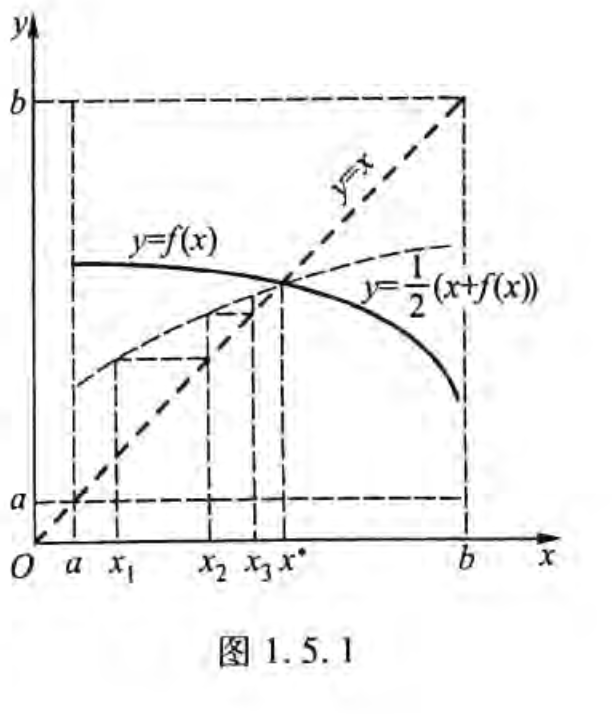
\includegraphics[width=0.42\textwidth]{1-5-1.png}
\end{center}

\subsection*{二、写出通项求极限}

\noindent\textbf{要点}\quad 对递推序列，有时可以通过递推关系写出数列的通项表达式，从而可以应用前几节的方法求极限.

\noindent\textbf{例 1.5.9}\quad 设 $x_0=0,x_1=1,x_{n+1}=\dfrac{x_n+x_{n-1}}{2}$，求 $\lim\limits_{n\to\infty}x_n$. （浙江大学）

\noindent\textbf{注}\quad 虽然可以证明此数列是压缩的，$\{x_n\}$ 收敛，但在递推公式里取极限，无法求出极限值. 但每项是前两项的算术平均值，因此从图 1.5.2 可以看出：$x_1=1,x_2=1-\dfrac12,x_3=1-\dfrac12+\dfrac14,x_4=1-\dfrac12+\dfrac14-\dfrac18,\cdots$，很容易写出 $x_n$ 的表达式.

\begin{center}
  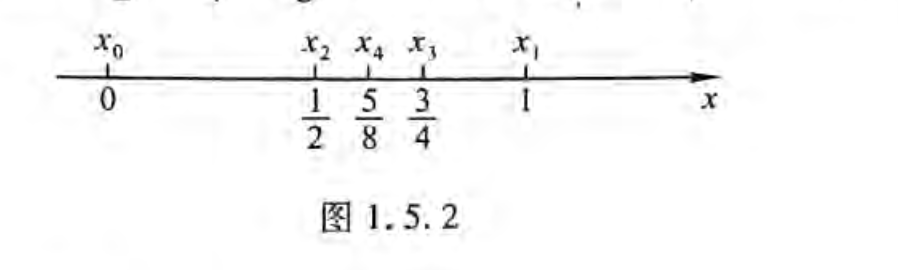
\includegraphics[width=0.38\textwidth]{1-5-2.png}
\end{center}

\noindent\textbf{解}\quad
\[
  x_{n+1}-x_n=\frac{x_n+x_{n-1}}{2}-x_n=-\frac{x_n-x_{n-1}}{2}.
\]
反复应用此结果，
\[
  x_{n+1}-x_n=\left(-\frac12\right)^n(x_1-x_0)=\frac{(-1)^n}{2^n}\quad (n=1,2,\cdots).
\]
于是
\[
\begin{aligned}
  x_{n+1}
  &=(x_{n+1}-x_n)+(x_n-x_{n-1})+\cdots+(x_1-x_0)+x_0\\
  &=\left(-\frac12\right)^n+\left(-\frac12\right)^{n-1}+\cdots+1\\
  &=\frac{1-\left(-\frac12\right)^{n+1}}{1-\left(-\frac12\right)}
  \to \frac23\quad (n\to\infty).
\end{aligned}
\]

\noindent\textbf{例 1.5.10}\quad 设 $a_1^{(0)},a_2^{(0)},a_3^{(0)}$ 为三角形各边的长，令
\[
\left\{
\begin{aligned}
  a_1^{(k)}&=\frac12(a_2^{(k-1)}+a_3^{(k-1)}),\\
  a_2^{(k)}&=\frac12(a_1^{(k-1)}+a_3^{(k-1)}),\\
  a_3^{(k)}&=\frac12(a_1^{(k-1)}+a_2^{(k-1)}),
\end{aligned}
\right.
\tag{1}
\]
证明：
\[
  \lim_{k\to\infty}a_i^{(k)}
  =\frac{a_1^{(0)}+a_2^{(0)}+a_3^{(0)}}{3}\quad (i=1,2,3).
\]
（南京大学）

\noindent\textbf{证}\quad （分别求 $a_i^{(k)}\ (i=1,2,3)$ 的表达式. ）由式 (1) 知
\[
  a_1^{(k)}+a_2^{(k)}+a_3^{(k)}
  =a_1^{(k-1)}+a_2^{(k-1)}+a_3^{(k-1)}
  =\cdots=a_1^{(0)}+a_2^{(0)}+a_3^{(0)}\stackrel{\text{记}}{=}l.
\]
且
\[
\begin{aligned}
  a_1^{(k)}
  &=\frac12(a_2^{(k-1)}+a_3^{(k-1)})\\
  &=\frac12\left[\frac12(a_1^{(k-2)}+a_3^{(k-2)})
    +\frac12(a_1^{(k-2)}+a_2^{(k-2)})\right]\\
  &=\frac{l}{4}+\frac14 a_1^{(k-2)}.
\end{aligned}
\]
由此
\[
  a_1^{(2k)}
  =\frac{l}{4}+\frac{l}{4^2}+\cdots+\frac{l}{4^k}
    +\frac{a_1^{(0)}}{4^k}
  =\frac{\frac{l}{4}-\frac{l}{4^{k+1}}}{1-\frac14}
    +\frac{a_1^{(0)}}{4^k}
  \to \frac{l}{3}\quad (k\to\infty).
\]
同理，$a_2^{(2k)}\to \dfrac{l}{3},a_3^{(2k)}\to \dfrac{l}{3}\ (k\to\infty)$. 故
\[
  a_1^{(2k+1)}=\frac12(a_2^{(2k)}+a_3^{(2k)})\to \frac{l}{3}\quad (k\to\infty).
\]
同理，$a_2^{(2k+1)}\to \dfrac{l}{3},a_3^{(2k+1)}\to \dfrac{l}{3}\ (k\to\infty)$. 故
\[
  \lim_{k\to\infty}a_i^{(k)}
  =\frac{l}{3}
  =\frac{a_1^{(0)}+a_2^{(0)}+a_3^{(0)}}{3}.
\]

通项并不总是轻而易举地能写出来，有时需要引入适当的参量.

\noindent\textbf{*例 1.5.11}\quad 设 $k>0,l>0,a_1,a_2$ 为已知常数，$a_1^2+a_2^2\ne 0$，数列 $\{a_n\}$ 由关系
\[
  a_{n+1}=ka_n+la_{n-1}
\tag{1}
\]
给出，试求 $\lim\limits_{n\to\infty}\dfrac{a_n}{a_{n-1}}$.

\noindent\textbf{解}\quad （我们先看看，假若 $\lim\limits_{n\to\infty}\dfrac{a_n}{a_{n-1}}$ 存在，其值应为什么？）在递推公式 (1) 中除以 $a_{n-1}$，得
\[
  \frac{a_{n+1}}{a_n}\cdot \frac{a_n}{a_{n-1}}
  =k\frac{a_n}{a_{n-1}}+l.
\tag{2}
\]
设 $\left\{\dfrac{a_n}{a_{n-1}}\right\}$ 收敛，记 $X=\lim\limits_{n\to\infty}\dfrac{a_n}{a_{n-1}}$，则由 (2) 得
\[
  X^2=kX+l,
\tag{3}
\]
解得
\[
  X_{1,2}=
  \begin{cases}
    \dfrac{k+\sqrt{k^2+4l}}{2}\stackrel{\text{记}}{=}\alpha,\\[6pt]
    \dfrac{k-\sqrt{k^2+4l}}{2}\stackrel{\text{记}}{=}\beta.
  \end{cases}
\]
显然 $\left|\dfrac{\beta}{\alpha}\right|<1$. （至此证明了：若所求的极限存在，则极限值必为 $\alpha$ 或 $\beta$. 为了证实该极限存在，自然希望把 $\dfrac{a_n}{a_{n-1}}$ 表示成 $\alpha,\beta$ 的函数，为此我们把递推公式里的 $k,l$ 变换成 $\alpha,\beta$. ）利用韦达定理，由式 (3)，
\[
  k=\alpha+\beta,\quad l=-\alpha\beta.
\]
代入递推公式 (1) 得
\[
  a_{n+1}-\alpha a_n=\beta(a_n-\alpha a_{n-1}),\quad
  a_{n+1}-\beta a_n=\alpha(a_n-\beta a_{n-1})\quad (n=2,3,\cdots),
\]
反复使用此式，得
\[
  a_{n+1}-\alpha a_n=\beta^{n-1}(a_2-\alpha a_1),\quad
  a_{n+1}-\beta a_n=\alpha^{n-1}(a_2-\beta a_1)\quad (n=2,3,\cdots).
\tag{4}
\]
可见：$1^\circ$ 若 $a_2=\beta a_1$，则 $\dfrac{a_{n+1}}{a_n}=\beta$，故 $\left\{\dfrac{a_{n+1}}{a_n}\right\}$ 收敛，$\lim\limits_{n\to\infty}\dfrac{a_n}{a_{n-1}}=\beta=\dfrac{k-\sqrt{k^2+4l}}{2}$.

$2^\circ$ 若 $a_2\ne \beta a_1$，则由式 (4) 可得
\[
  a_{n+1}
  =\frac{\alpha^n(a_2-\beta a_1)-\beta^n(a_2-\alpha a_1)}{\alpha-\beta}.
\]
从而可写出 $\dfrac{a_{n+1}}{a_n}$ 的表达式：
\[
  \frac{a_{n+1}}{a_n}
  =\frac{\alpha^n(a_2-\beta a_1)-\beta^n(a_2-\alpha a_1)}
    {\alpha^{n-1}(a_2-\beta a_1)-\beta^{n-1}(a_2-\alpha a_1)}
  =\frac{\alpha\left(\dfrac{\alpha}{\beta}\right)^{n-1}
      -\beta\dfrac{a_2-\alpha a_1}{a_2-\beta a_1}}
    {\left(\dfrac{\alpha}{\beta}\right)^{n-1}
      -\dfrac{a_2-\alpha a_1}{a_2-\beta a_1}}.
\]
注意 $\left|\dfrac{\alpha}{\beta}\right|>1$，$n$ 充分大时，
\[
  \left|\frac{\alpha}{\beta}\right|^{n-1}
  >\left|\frac{a_2-\alpha a_1}{a_2-\beta a_1}\right|,
\]
故
\[
  \lim_{n\to\infty}\frac{a_{n+1}}{a_n}
  =\alpha=\frac{k+\sqrt{k^2+4l}}{2}\quad (n\to\infty).
\]
解毕.

为了写出通项，有时可联系对偶的问题来考虑（这也是数学中常用的思想方法），如下例.

\noindent\textbf{*例 1.5.12}\quad 设 $[x]$ 表示不超过 $x$ 的最大整数，记号 $\{x\}=x-[x]$ 表示 $x$ 的小数部分，试求
\[
  \lim_{n\to\infty}\{(2+\sqrt3)^n\}. \quad \text{（国外赛题）}
\]

\noindent\textbf{解}\quad $\{(2+\sqrt3)^n\}$ 是 $(2+\sqrt3)^n$ 的小数部分，自然，将 $(2+\sqrt3)^n$ 中的整数项去掉，不会影响它的值. 将 $(2+\sqrt3)^n$ 展开，合并同类项：
\[
  (2+\sqrt3)^n=\sum_{k=0}^n C_n^k(\sqrt3)^k2^{n-k}=A_n+B_n\sqrt3,
\tag{1}
\]
其中 $A_n$ 表示 $k$ 为偶数的各项之和，$B_n\sqrt3$ 是 $k$ 为奇数的各项之和，可见 $A_n,B_n$ 都是整数. 去掉第一项 $A_n$，不影响小数部分，
\[
  \{(2+\sqrt3)^n\}=\{B_n\sqrt3\}.
\tag{2}
\]
为了进一步求 $\{B_n\sqrt3\}$ 的表达式，打开思路，考虑对偶问题. 与式 (1) 比较，有
\[
  0<(2-\sqrt3)^n=A_n-B_n\sqrt3.
\tag{3}
\]
由此，我们发现，$B_n\sqrt3<A_n$，即 $A_n$ 是比无理数 $B_n\sqrt3$ 大的整数，而且式 (3) 中 $0<2-\sqrt3<1$，故由式 (3)，
\[
  A_n-B_n\sqrt3=(2-\sqrt3)^n\to 0\quad (n\to\infty).
\tag{4}
\]
这说明 $A_n$ 不仅是比 $B_n\sqrt3$ 大的整数，而且是与 $B_n\sqrt3$ 无限接近的整数. 故 $B_n\sqrt3$ 的小数部分 $\{B_n\sqrt3\}=B_n\sqrt3-(A_n-1)$. 联系式 (2) 和 (4)，
\[
  \{(2+\sqrt3)^n\}=\{B_n\sqrt3\}
  =B_n\sqrt3-(A_n-1)
  =1-(A_n-B_n\sqrt3)\to 1\quad (n\to\infty).
\]

\subsection*{三、替换与变形}

\noindent\textbf{要点}\quad 对递推形式的数列，同样可以进行变量替换与变形，使之变成已知极限，或易于计算的极限.

\noindent\textbf{例 1.5.13}\quad 设 $\{a_n\}$ 为 Fibonacci 数列，即 $a_1=1,a_2=1,a_{n+2}=a_{n+1}+a_n\ (n=1,2,\cdots)$. 记
\[
  x_n=\frac{a_{n+1}}{a_n},
\]
求 $\lim\limits_{n\to\infty}x_n$. （华中师范大学）

\noindent\textbf{解}\quad 由已知条件知
\[
  \frac{a_{n+2}}{a_{n+1}}=1+\frac{a_n}{a_{n+1}},
\]
即
\[
  x_{n+1}=1+\frac1{x_n}.
\]
令 $y_n=\dfrac1{x_n}$，此即
\[
  y_{n+1}=\frac1{1+y_n},
\]
且 $y_1=\dfrac1{x_1}=\dfrac{a_1}{a_2}=1$. 这就是本节例 1.5.4. 故
\[
  \lim_{n\to\infty}y_n=0.618\cdots,
\]
从而
\[
  \lim_{n\to\infty}x_n
  =\lim_{n\to\infty}\frac1{y_n}
  =\lim_{n\to\infty}(1+y_n)
  =1.618\cdots.
\]

\noindent\textbf{例 1.5.14}\quad 证明数列
\[
  2,\ 2+\frac12,\ 2+\frac{1}{2+\frac12},\ \cdots
\]
收敛，并求其极限. （华中科技大学）

\noindent\textbf{解}\quad 从数列特征可以看出，相邻两项的关系是
\[
  x_{n+1}=2+\frac1{x_n}.
\tag{1}
\]
因此，设 $\{x_n\}$ 收敛，则极限 $A$ 满足方程 $A=2+\dfrac1A$，考虑到 $x_n>0$，所以 $A=1+\sqrt2$. 要证明 $\{x_n\}$ 以 $A$ 为极限，亦即
\[
  x_n=A+\alpha_n=1+\sqrt2+\alpha_n.
\tag{2}
\]
将式 (2) 代入式 (1) 得
\[
  \alpha_{n+1}=\frac{(1-\sqrt2)\alpha_n}{1+\sqrt2+\alpha_n}.
\tag{3}
\]
至此，我们已将满足式 (1) 的数列 $\{x_n\}\to A$ 的问题，化为满足式 (3) 的数列 $\{\alpha_n\}\to 0$ 的问题. 事实上，
\[
  \alpha_1=x_1-A=1-\sqrt2,\qquad |\alpha_1|<\frac12.
\]
应用数学归纳法，由式 (3) 易证 $|\alpha_n|<\dfrac1{2^n}$. 故
\[
  \lim_{n\to\infty}x_n
  =\lim_{n\to\infty}(1+\sqrt2+\alpha_n)
  =1+\sqrt2.
\]

\noindent\textbf{另解}\quad 因 $x_n\ge 2\ (\forall n\in\mathbb{N})$，
\[
  |x_{n+1}-x_n|
  =\left|\frac1{x_n}-\frac1{x_{n-1}}\right|
  =\frac{|x_{n-1}-x_n|}{|x_nx_{n-1}|}
  \le \frac14 |x_n-x_{n-1}|,
\]
故 $\{x_n\}$ 收敛，极限 $A$：$A=2+\dfrac1A$，得 $A=1+\sqrt2$.

\subsection*{四、图解法}

上面几种解法都是分析解法，论证严谨，思想性强，但不够直观. 下面提出一种图解法，可给人以整体观念，做到一目了然. 有些问题，此法可帮助我们看出 $\{a_n\}$ 的变化情况.

\noindent\textbf{要点}\quad 设 $y=f(x)$ 为严格单调的连续函数，$a_1$ 已给定且 $a_n=f(a_{n-1})$. 为求 $\lim\limits_{n\to\infty}a_n$，在 $xOy$ 平面上作出函数 $y=f(x)$ 及其反函数 $y=g(x)$ 的图像，如图 1.5.3. 在 $x$ 轴上取点 $A_1$，使横坐标为 $x=a_1$，过 $A_1$ 作竖直线，与 $y=f(x)$ 的图像交于点 $A_2$，则 $A_2$ 的纵坐标 $y=f(a_1)=a_2$；过 $A_2$ 作水平直线与 $y=g(x)$ 的图像交于点 $A_3$，则 $A_3$ 的横坐标
\[
  x=g^{-1}(y)\big|_{y=a_2}=f(a_2)=a_3.
\]
过 $A_3$ 作竖直线与 $y=f(x)$ 的图像交于点 $A_4,\cdots$；如此无限进行下去. 例如图 1.5.3 所示的情况，点 $A_n$ 的极限位置 $A^*$ 是 $y=f(x),y=g(x)$（及 $y=x$）的交点，$A^*$ 的坐标
\[
  x^*=f(x^*)
\]
便是 $\{a_n\}$ 的极限.

\begin{center}
  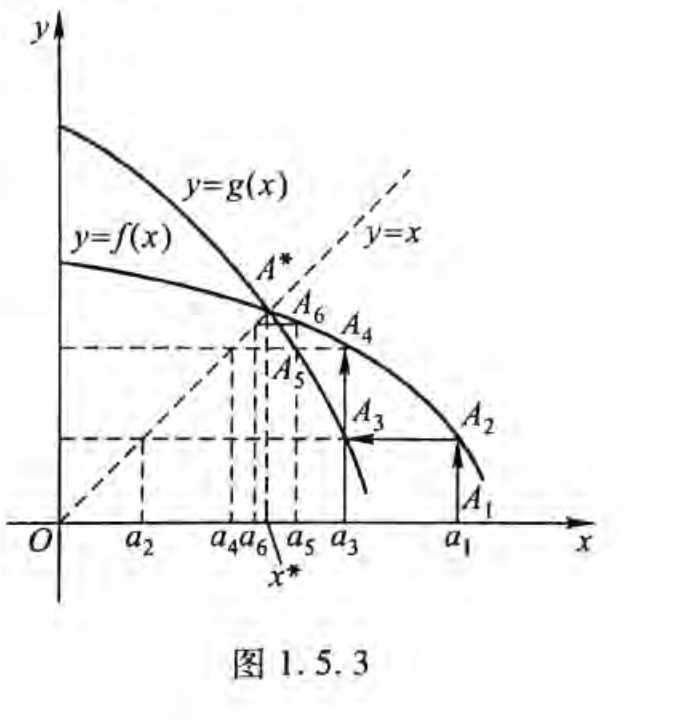
\includegraphics[width=0.42\textwidth]{1-5-3.png}
\end{center}

\noindent\textbf{*例 1.5.15}\quad 设 $y=f(x)=\dfrac1{1+x},a_1=1,a_{n+1}=f(a_n)$，求 $\lim\limits_{n\to\infty}a_n$.

按此法在 $x$ 轴上得
\[
  a_1>a_3>a_5>\cdots>a_{2n+1}>\cdots>x^*;
\]
在 $y$ 轴上得
\[
  a_2<a_4<\cdots<a_{2n}<\cdots<x^*,
\]
极限满足方程
\[
  x^*=\frac1{1+x^*},
\]
故
\[
  x^*=\frac{-1+\sqrt5}{2}=0.618\cdots.
\]
图 1.5.4 就是按本题作出的. 从图上不难看出，当 $a_1$ 取 $x>x^*$ 的任意一值时，所得结果与 $a_1=1$ 的情况相同，$\{a_{2n}\}\nearrow x^*,\{a_{2n+1}\}\searrow x^*$. 当 $a_1<x^*$ 时，情况是 $\{a_{2n}\}\searrow x^*,\{a_{2n+1}\}\nearrow x^*$. 当 $a_1=x^*$ 时，一切 $a_n=x^*$.

\begin{center}
  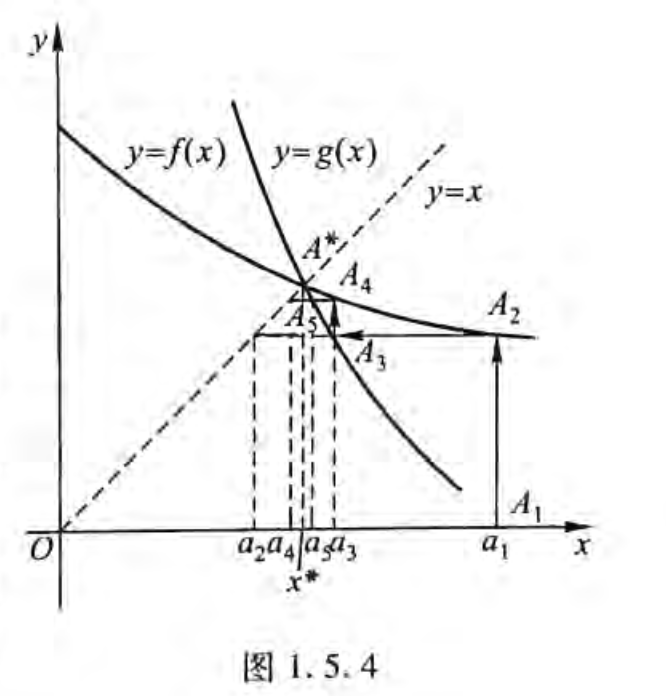
\includegraphics[width=0.42\textwidth]{1-5-4.png}
\end{center}

\noindent\textbf{*例 1.5.16（切线法逼近求根）}\quad 设 $f(x)$ 在 $[a,b]$ 上二次可微，且 $f(a)\cdot f(b)<0,f'(x)>0,f''(x)>0,\forall x\in [a,b]$. 证明：
\[
  x_{n+1}=x_n-\frac{f(x_n)}{f'(x_n)},\quad x_1\in [a,b],\quad n=1,2,\cdots
\tag{1}
\]
有极限，且此极限为方程 $f(x)=0$ 之根. （中国科学技术大学）

\noindent\textbf{证}\quad 因 $f$ 在 $[a,b]$ 两端点异号，$[a,b]$ 上 $f'(x)>0$，故 $f(x)=0$ 在 $(a,b)$ 内存在唯一的根 $c$，$f(c)=0$. （下面的目标证明 $\lim\limits_{n\to\infty}x_n=c$. ）由 $f'(x)>0$，改写式 (1)：
\[
  0<f'(x_n)=\frac{f(x_n)}{x_n-x_{n+1}}
  =\frac{f(x_n)-f(c)}{x_n-x_{n+1}}
  =\frac{f'(\xi_n)(x_n-c)}{x_n-x_{n+1}},
\tag{2}
\]
（$\xi_n$ 在 $x_n$ 与 $c$ 之间）. 此式表明：若能证明
\[
  x_n>c\quad (n=2,3,\cdots),
\tag{3}
\]
则必有 $x_n>x_{n+1}\ (n=2,3,\cdots)$. 从而 $x_n$ 递减有下界，故有极限，记为 $A$. 由式 (1) 取极限，可知 $f(A)=0,A=c$. 下面来证不等式 (3). 事实上，利用微分中值定理，有
\[
\begin{aligned}
  x_{n+1}-c
  &\stackrel{(1)}{=}x_n-c-\frac{f(x_n)-f(c)}{f'(x_n)}\\
  &=(x_n-c)\left[1-\frac{f'(\eta_n)}{f'(x_n)}\right]\\
  &=(x_n-c)\frac{f'(x_n)-f'(\eta_n)}{f'(x_n)}
   =(x_n-c)\frac{f''(\xi_n)(x_n-\eta_n)}{f'(x_n)},
\end{aligned}
\tag{4}
\]
其中 $\eta_n$ 在 $x_n$ 与 $c$ 之间，$\xi_n$ 在 $x_n$ 与 $\eta_n$ 之间. 因 $f',f''>0$，故可推知 $x_{n+1}>c$（不论 $x_n>c$ 或 $x_n<c$）. 因此，若 $x_1>c$，则一切 $x_n>c$；若 $x_1<c$，则 $x_2,x_3,\cdots>c$.

最后若 $x_1=c$，显然一切 $x_n=c$，亦有 $\lim x_n=c$.

\noindent\textbf{注}\quad 本例的几何意义是用切线法逼近求根. 因为 $f'(x_n)=\tan\alpha$，其中 $\alpha$ 是曲线 $y=f(x)$ 在 $(x_n,f(x_n))$ 处的切线与 $x$ 轴的夹角. 如图 1.5.5，可知
\[
  f(x_n)=(x_n-x_{n+1})\tan\alpha=(x_n-x_{n+1})f'(x_n),
\]
这就是式 (1).

利用此式进行迭代可求 $f(x)=0$ 的根的近似值.

\begin{center}
  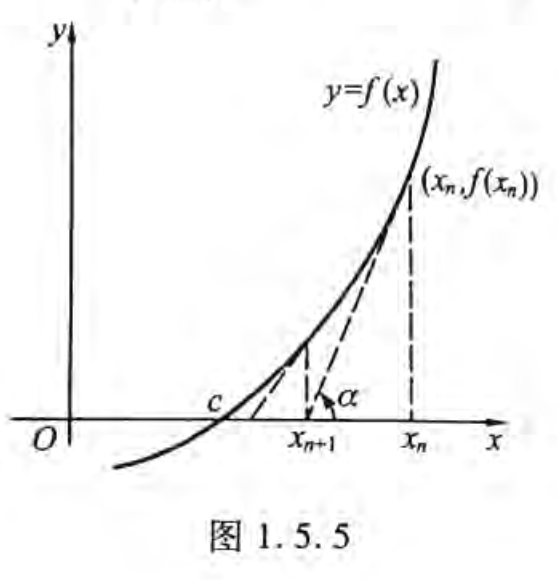
\includegraphics[width=0.42\textwidth]{1-5-5.png}
\end{center}

\subsection*{五、不动点方法的推广}

设 $z=f(x,y)$ 为二元函数，我们约定，将 $z=f(x,x)$ 的不动点称为 $f$ 的不动点（或二元不动点）.

\noindent\textbf{*例 1.5.17}\quad 已知 $z=f(x,y)$ 为 $x>0,y>0$ 上定义的正连续函数，$z$ 分别对 $x$ 和 $y$ 单调递增，假若：（1）存在点 $b$ 是 $f(x,x)$ 的不动点；（2）当且仅当 $x>b$ 时有 $x>f(x,x)$. 令 $a_1=f(a,a),a_2=f(a_1,a)\ (a>0)$，
\[
  a_n=f(a_{n-1},a_{n-2})\quad (n=3,4,\cdots),
\tag{1}
\]
试证 $\{a_n\}$ 单调有界，有极限，且其极限 $A$ 是 $f$ 的不动点.

\noindent\textbf{证}\quad 只需证明 $\{a_n\}$ 收敛. 因为这样就可在式 (1) 中取极限，知 $A$ 是 $f$ 的不动点. 下面分两种情况进行讨论：

$1^\circ$ 若 $a\le a_1$. 由 $f$ 对 $x$ 和 $y$ 的单增性知 $a_2=f(a_1,a)\ge f(a,a)=a_1$，进而 $a_3=f(a_2,a_1)\ge f(a_1,a)=a_2$. 类似：若已推得 $a_{n-1}\ge a_{n-2},a_n\ge a_{n-1}$，则
\[
  a_{n+1}=f(a_n,a_{n-1})\ge f(a_{n-1},a_{n-2})=a_n\quad (n=3,4,\cdots),
\]
如此得 $\{a_n\}$ 递增（单调递增）.

又因 $a_1=f(a,a)\ge a$，按已知条件，这时只能 $a\le b$（否则 $a>b$，按已知条件 (2)，应有 $a>f(a,a)=a_1$，产生矛盾），进而 $a_1=f(a,a)\le f(b,b)=b,a_2=f(a_1,a)\le f(b,a)\le f(b,b)=b,\cdots$，用数学归纳法可得一切 $a_n\le b$. 总之 $\{a_n\}$ 单调递增有上界，故 $\{a_n\}$ 收敛.

$2^\circ$ 若 $a_1\le a$. 类似可证 $\{a_n\}$ 递减有下界 $b$，$\{a_n\}$ 收敛.

\noindent\textbf{注}\quad 按 $b$ 的条件可知 $b$ 是 $f$ 的最大不动点，$x>b$ 时不可能再有不动点. 情况 $2^\circ$ 时极限 $A\ge b$ 是不动点，表明此时 $A=b$.

\noindent\textbf{*例 1.5.18}\quad 若 $a>0$，
\[
  a_1=(a+a^{1/3})^{1/3},\quad
  a_2=(a_1+a^{1/3})^{1/3},\quad \cdots,\quad
  a_n=(a_{n-1}+a_{n-2}^{1/3})^{1/3},\quad \cdots,
\]
试证：

1）数列 $\{a_n\}$ 为单调有界数列；

2）数列 $\{a_n\}$ 收敛于方程 $x^3=x+x^{1/3}$ 的一个正根. （广西师范大学）

\noindent\textbf{证}\quad （利用上例. ）设 $z=f(x,y)=(x+y^{1/3})^{1/3}$，显然 $f$ 当 $x>0,y>0$ 时是正值连续函数，对 $x,y$ 单调递增，只需证明：（1）$\exists b$ 使得 $b=f(b,b)$；（2）$x>f(x,x)$ 当且仅当 $x>b$.

$1^\circ$ 注意到 $f$ 的不动点亦是方程 $x^3-x-x^{1/3}=0$ 的根. 分析函数 $g(x)=x^3-x-x^{1/3}$，因
\[
  g'(x)=3x^2-1-\frac1{3x^{2/3}},\qquad
  g''(x)=6x+\frac{2}{9x^{5/3}}>0\quad (x>0),
\]
$g'(0+0)=-\infty,g'(1)>0$，可知 $g$ 在 $(0,1)$ 内有唯一极小点 $c$. $x>c$ 时 $g'(x)>0,g$ 严增，$g(1)<0,g(2)>0$，故 $g$ 在 $(0,1)$ 内有唯一零点 $b$（即 $f$ 的不动点）.

$2^\circ$ $x>b$ 时 $g(x)>g(b)=0$，即 $x>f(x,x)$. 事实上，在 $x>0$ 的范围内也只有在 $x>b$ 时才有 $x>f(x,x)$；因为 $g(0)=0,g(b)=0$，在 $(0,c)$ 上 $g(x)$ 严减，$(c,b)$ 上 $g(x)$ 严增，所以 $(0,b)$ 内 $g(x)<0$，即 $x<f(x,x)$.

\subsection*{六、Stolz 公式的应用}

\noindent\textbf{例 1.5.19}\quad 对于数列 $x_0=a,0<a<\dfrac{\pi}{2},x_n=\sin x_{n-1}\ (n=1,2,\cdots)$，证明：

1）$\lim\limits_{n\to\infty}x_n=0$；

2）$\lim\limits_{n\to\infty}\sqrt{\dfrac{n}{3}}x_n=1$. （复旦大学，中国人民大学）

\noindent\textbf{证}\quad 1）因 $0<a<\dfrac{\pi}{2},x_0=a$，递推可知
\[
  0<x_n=\sin x_{n-1}<x_{n-1}<\frac{\pi}{2}\quad (n=1,2,\cdots),
\]
表明 $x_n$ 递减有下界 $0$，$\lim\limits_{n\to\infty}x_n$ 存在. 记 $\lim\limits_{n\to\infty}x_n=A$，知 $A=\sin A,A=0,\lim\limits_{n\to\infty}x_n=0$.

2）（用 Stolz 公式. ）要证 $\lim\limits_{n\to\infty}\sqrt{\dfrac{n}{3}}x_n=1$，即要证
\[
  \lim_{n\to\infty} nx_n^2=3
  \quad\text{或}\quad
  \lim_{n\to\infty}\frac{n}{1/x_n^2}=3.
\]
用 $\dfrac{\infty}{\infty}$ 型 Stolz 公式，
\[
\begin{aligned}
  \lim_{n\to\infty}\frac{n}{1/x_n^2}
  &=\lim_{n\to\infty}\frac{n-(n-1)}{1/x_n^2-1/x_{n-1}^2}\\
  &=\lim_{n\to\infty}\frac{1}{1/\sin^2 x_{n-1}-1/x_{n-1}^2}\\
  &=\lim_{n\to\infty}\frac{x_{n-1}^2\sin^2 x_{n-1}}{x_{n-1}^2-\sin^2 x_{n-1}}\\
  &=\lim_{x\to 0}\frac{x^2\sin^2 x}{x^2-\sin^2 x}
   =\lim_{x\to 0}\frac{x^4}{(x+\sin x)(x-\sin x)}\\
  &=\lim_{x\to 0}\frac{x^4}{(2x+o(x))\left(\frac{x^3}{6}+o(x^3)\right)}
   =\lim_{x\to 0}\frac{1}{(2+o(1))\left(\frac16+o(1)\right)}
   =3.
\end{aligned}
\]

\noindent\textbf{例 1.5.20}\quad 设 $0<x_1<1,x_{n+1}=x_n(1-x_n),n=1,2,\cdots$，证明：

1）$\lim\limits_{n\to\infty}x_n=0$；

2）$\lim\limits_{n\to\infty}nx_n=1$. （北京师范大学）

\noindent\textbf{提示}\quad 1）$0<x_n<1\ (n=1,2,\cdots)$，$x_{n+1}-x_n=-x_n^2<0$，$x_n$ 递减.

2）
\[
  \lim_{n\to\infty}nx_n
  =\lim_{n\to\infty}\frac{n-(n-1)}{1/x_n-1/x_{n-1}}
  =\lim_{n\to\infty}\frac{1}{\frac1{x_{n-1}(1-x_{n-1})}-\frac1{x_{n-1}}}.
\]

\noindent\textbf{new 练习 1}\quad 求
\[
  \lim_{n\to\infty}\left(1+\frac12+\frac13+\cdots+\frac1n\right)^{1/n}.
\]
（华中科技大学）\hfill $\langle 1\rangle$

\noindent\textbf{提示}\quad 取对数，应用 Stolz 公式.

\noindent\textbf{再提示}\quad
\[
\begin{aligned}
  &\lim_{n\to\infty}\ln\left(1+\frac12+\frac13+\cdots+\frac1n\right)^{1/n}\\
  &=\lim_{n\to\infty}\frac1n\ln\left(1+\frac12+\frac13+\cdots+\frac1n\right)\\
  &\stackrel{\mathrm{Stolz}}{=}
    \lim_{n\to\infty}\ln
    \frac{1+\frac12+\frac13+\cdots+\frac1n}
         {1+\frac12+\frac13+\cdots+\frac1{n-1}}\\
  &=\ln\left(\lim_{n\to\infty}
    \frac{1+\frac12+\frac13+\cdots+\frac1{n-1}+\frac1n}
         {1+\frac12+\frac13+\cdots+\frac1{n-1}}\right)
   \stackrel{\mathrm{Stolz}}{=}\ln 1=0.
\end{aligned}
\]

\noindent\textbf{new 练习 2}\quad 已知数列 $\{a_n\}$ 满足：
\[
  \lim_{n\to\infty}\frac{a_{2n}}{2n}=a,\qquad
  \lim_{n\to\infty}\frac{a_{2n+1}}{2n+1}=b,
\]
试证：
\[
  \lim_{n\to\infty}\frac{a_1+a_2+\cdots+a_n}{1+2+\cdots+n}
  =\frac{a+b}{2}.
\]
（中国科学技术大学）

\noindent\textbf{提示}\quad 应用 Stolz 公式，根据例 1.2.13，对奇项和偶项分别证明成立即可.

\noindent\textbf{再提示}\quad 记
\[
  x_n=\frac{a_1+a_2+\cdots+a_n}{1+2+\cdots+n},
\]
则
\[
  x_{2n}
  =\frac{a_1+a_3+\cdots+a_{2n-1}}{1+2+\cdots+2n}
   +\frac{a_2+a_4+\cdots+a_{2n}}{1+2+\cdots+2n}
  \stackrel{\text{记}}{=}x'_{2n}+x''_{2n},
\]
且
\[
  \lim_{n\to\infty}x'_{2n}
  =\lim_{n\to\infty}
    \frac{a_1+a_3+\cdots+a_{2n-1}}
         {1+2+\cdots+2n}
  =\lim_{n\to\infty}
    \frac{a_1+a_3+\cdots+a_{2n-1}}
         {(1+2)+(3+4)+\cdots+(2n-1+2n)}
  \stackrel{\mathrm{Stolz}}{=}
    \lim_{n\to\infty}\frac{2n-1}{(2n-1)+2n}\cdot \frac{a_{2n-1}}{2n-1}
  =\frac{b}{2}.
\]
同理可证：
\[
  \lim_{n\to\infty}x''_{2n}=\frac{a}{2},
\]
于是
\[
  \lim_{n\to\infty}x_{2n}
  =\lim_{n\to\infty}(x'_{2n}+x''_{2n})
  =\frac{a+b}{2}.
\]
类似可证：
\[
  \lim_{n\to\infty}x_{2n+1}=\frac{a+b}{2}
\]
（只需定义 $a_0=0$（不影响敛散性和极限值），并将 $x_{2n+1}$ 写成
\[
  x_{2n+1}
  =\frac{a_1+a_3+\cdots+a_{2n+1}}{(0+1)+(2+3)+\cdots+(2n+2n+1)}
   +\frac{0+a_2+a_4+\cdots+a_{2n}}{(0+1)+(2+3)+\cdots+(2n+2n+1)}.
\]

\subsection*{七、递推极限的直接法}

\noindent\textbf{要点}\quad 递推数列如果有极限，在递推公式里两端同时求极限，可得到关于极限值的方程式. 因此，只需直接检验：该数列是否趋向此方程的实根？一是，则数列收敛，并且此实根就是所求的极限（值）；否则数列发散.

\noindent\textbf{new 例 1.5.21}\quad 设 $x_0\in\left(1,\dfrac32\right),x_1=x_0^2$，
\[
  x_{n+1}=\sqrt{x_n}+\frac{x_{n-1}}2,\quad n=1,2,\cdots,
\]
求证数列 $\{x_n\}$ 收敛，并求极限. （中国科学技术大学）

\noindent\textbf{思想}\quad 假设 $\lim\limits_{n\to\infty}x_n$ 存在，记为 $a$，在原式里取极限得
\[
  a=\sqrt a+\frac a2,
\]
解方程得 $a=4$ 和 $a=0$. 但 $\forall n:x_n\ge 1$，故 $a\ne 0$. 只需验证是否有：
\[
  \lim_{n\to\infty}|x_n-4|=0.
\]

\noindent\textbf{解 I}\quad
\[
\begin{aligned}
  |x_n-4|
  &=\left|\sqrt{x_{n-1}}+\frac{x_{n-2}}2-4\right|\\
  &\le |\sqrt{x_{n-1}}-2|+\frac{|x_{n-2}-4|}{2}\\
  &=\left|\frac{x_{n-1}-4}{\sqrt{x_{n-1}}+2}\right|
    +\frac{|x_{n-2}-4|}{2}\\
  &\le \frac12\bigl(|x_{n-1}-4|+|x_{n-2}-4|\bigr).
\end{aligned}
\]
（再对 $|x_{n-1}-4|$ 应用此结果）
\[
\begin{aligned}
  |x_n-4|
  &\le \frac1{2^2}\bigl(3|x_{n-2}-4|+|x_{n-3}-4|\bigr)\\
  &\le \frac1{2^3}\bigl(5|x_{n-3}-4|+3|x_{n-4}-4|\bigr)
   \quad \text{（继续迭代）}\\
  &\le \cdots \le
   \frac1{2^{n-1}}\bigl[(2n-1)|x_1-4|+(2n-3)|x_0-4|\bigr]\\
  &\le \frac1{2^{n-1}}\bigl[(2n)\cdot 3+(2n)\cdot 3\bigr]
   \le \frac{n}{2^{n-5}}\to 0\quad (n\to\infty).
\end{aligned}
\]

\noindent\textbf{解 II}\quad
$1^\circ$ 用数学归纳法可证：$1<x_n<4$，且 $\{x_n\}$ 递增.

事实上，已有：$1<x_0,x_1<4$；若 $1<x_{n-1},x_n<4$，则
\[
  x_{n+1}=\sqrt{x_n}+\frac{x_{n-1}}2
  >\sqrt1+\frac12>1,\qquad
  x_{n+1}=\sqrt{x_n}+\frac{x_{n-1}}2
  <\sqrt4+\frac42=4.
\]
因此，$1<x_n<4$，$\{x_n\}$ 有界.

另一方面，由 $1<x_0<x_0^2=x_1$ 知：
\[
  \frac{x_2}{x_1}
  =\frac{\sqrt{x_1}+\frac{x_0}{2}}{x_1}
  =\frac{3}{2x_0}>1,
\]
故 $x_1<x_2$. 设已证 $x_{n-2}<x_{n-1}<x_n$，则有
\[
\begin{aligned}
  x_{n+1}-x_n
  &=\left(\sqrt{x_n}+\frac{x_{n-1}}2\right)
    -\left(\sqrt{x_{n-1}}+\frac{x_{n-2}}2\right)\\
  &=(\sqrt{x_n}-\sqrt{x_{n-1}})
    +\frac{x_{n-1}-x_{n-2}}2>0,
\end{aligned}
\]
亦即 $x_{n-1}<x_n<x_{n+1}$. 因此 $x_n$ 递增.

$2^\circ$ 根据单调有界原理，令 $\lim\limits_{n\to\infty}x_n=a$. 在
\[
  x_{n+1}=\sqrt{x_n}+\frac{x_{n-1}}2
\]
里取极限，得 $a=\sqrt a+\dfrac a2,a=4$.

\noindent\textbf{new *例 1.5.22}\quad 设 $0<a_1,b_1<1$，当 $n\ge 2$ 时，
\[
  a_n=\frac{1+b_{n-1}^2}{2},\qquad
  b_n=a_{n-1}-\frac{a_{n-1}^2}{2}.
\tag{1}
\]
试证 $\{a_n\},\{b_n\}$ 收敛，并求它们的极限.

\noindent\textbf{解 I}\quad
$1^\circ$ $n\ge 2$ 时，
\[
  a_n=\frac{1+b_{n-1}^2}{2}\ge \frac12,\qquad
  0<b_n=a_{n-1}-\frac{a_{n-1}^2}{2}
  =\frac12-\frac{(a_{n-1}-1)^2}{2}\le \frac12,
\]
从而
\[
  \frac12\le a_{n+1}=\frac{1+b_n^2}{2}\le \frac58,\qquad
  \frac12\ge b_{n+1}=\frac12-\frac{(a_n-1)^2}{2}\ge \frac38.
\]
可见，当 $n\ge 3$ 时，
\[
  \frac12\le a_n\le \frac58,\qquad \frac12\ge b_n\ge \frac38.
\tag{2}
\]

$2^\circ$ 若 $\{a_n\},\{b_n\}$ 收敛，极限分别记为 $a$ 和 $b$. 在式 (1) 里取极限，得
\[
  a=\frac{1+b^2}{2},
\tag{3}
\]
\[
  b=a-\frac{a^2}{2}.
\tag{4}
\]
式 (4) 改写为
\[
  \frac{a^2}{2}=a-b\stackrel{(3)}{=}
  \frac{1+b^2-2b}{2}
  =\frac{(1-b)^2}{2},
\]
故 $a=1-b$（$a=-(1-b)$ 舍去）. 代入式 (3)，解得 $b=-1\pm\sqrt2$. 由式 (2) 可知 $a\ge \dfrac12,b\ge \dfrac38$，故
\[
  b=\sqrt2-1,\qquad a=2-\sqrt2.
\tag{5}
\]
这说明 $\{a_n\},\{b_n\}$ 如果收敛，那么极限必是此二数.

至此，只需验证 $(n\to\infty)$：$|a_n-a|\to 0$ 和 $|b_n-b|\to 0$.

$3^\circ$ 利用式 (1) 至式 (5)：
\[
\begin{aligned}
  |a_n-a|
  &=\frac12|b_{n-1}^2-b^2|
   =\frac12|b_{n-1}+b|\,|b_{n-1}-b|
   \le \frac12|b_{n-1}-b|,\\
  |b_n-b|
  &=\left|a_{n-1}-a-\frac{a_{n-1}^2-a^2}{2}\right|\\
  &=|a_{n-1}-a|
    \left|\frac{2-(a_{n-1}+a)}2\right|
   \le \frac12|a_{n-1}-a|
  \quad (\text{因 }|2-(a_{n-1}+a)|\le 1).
\end{aligned}
\]
两式迭代得
\[
  |a_n-a|\le \frac14 |a_{n-2}-a|,
\tag{6}
\]
\[
  |b_n-b|\le \frac14 |b_{n-2}-b|.
\tag{7}
\]
用式 (6) 进行迭代，可得
\[
  |a_{2n}-a|\le \frac1{4^{n-1}}|a_2-a|,\qquad
  |a_{2n+1}-a|\le \frac1{4^{n-1}}|a_3-a|.
\]
可见 $\{a_n\}$ 收敛，$\lim\limits_{n\to\infty}a_n=a=2-\sqrt2$.

类似地，有 $\lim\limits_{n\to\infty}b_n=b=\sqrt2-1$.

\noindent\textbf{解 II}\quad 同上. $\forall n$：
\[
  1>a_n=\frac{1+b_{n-1}^2}{2}\ge \frac12,
\tag{8}
\]
\[
  0<b_n=a_{n-1}-\frac{a_{n-1}^2}{2}
  =\frac12-\frac{(a_{n-1}-1)^2}{2}\le \frac12.
\tag{9}
\]
故
\[
\begin{aligned}
  |a_n-a_{n-1}|
  &=\frac12|b_{n-1}^2-b_{n-2}^2|
   =\frac12|b_{n-1}+b_{n-2}|\,|b_{n-1}-b_{n-2}|
   \stackrel{(9)}{\le}\frac12|b_{n-1}-b_{n-2}|.
\end{aligned}
\]
类似地，
\[
\begin{aligned}
  |b_n-b_{n-1}|
  &=\left|a_{n-1}-a_{n-2}
    -\left(\frac{a_{n-1}^2}{2}-\frac{a_{n-2}^2}{2}\right)\right|\\
  &=|a_{n-1}-a_{n-2}|
    \left|\frac{2-(a_{n-1}+a_{n-2})}{2}\right|
   \stackrel{(8)}{\le}\frac12|a_{n-1}-a_{n-2}|.
\end{aligned}
\]
迭代即得
\[
  |a_n-a_{n-1}|\le \frac14|a_{n-2}-a_{n-3}|,\qquad
  |b_n-b_{n-1}|\le \frac14|b_{n-2}-b_{n-3}|.
\]
于是
\[
  |a_{2n}-a_{2n-1}|
  \le \frac1{4^{n-1}}|a_2-a_1|
  \le \frac12\cdot \frac1{4^{n-1}}
  =\frac1{2^{2n-1}},
\]
\[
  |a_{2n+1}-a_{2n}|
  \le \frac1{4^{n-1}}|a_3-a_2|
  \le \frac1{4^{n-1}}\cdot \frac12|b_2-b_1|
  =\frac1{2^{2n}}.
\]
由此得 $\{a_n\}$ 和 $\{b_n\}$ 收敛，解方程 (3) 和 (4)，可得式 (5).

\noindent\textbf{new *例 1.5.23}\quad 设 $a_1,b_1$ 为任意选定的两实数，$a_n,b_n$ 定义如下：
\[
  a_n=\int_0^1 \max\{b_{n-1},x\}\,dx,\qquad
  b_n=\int_0^1 \min\{a_{n-1},x\}\,dx\quad (n=2,3,\cdots).
\tag{1}
\]
试证：
\[
  \lim_{n\to\infty}a_n=2-\sqrt2,\qquad
  \lim_{n\to\infty}b_n=\sqrt2-1.
\]
（浙江大学）

\noindent\textbf{证}\quad 令 $a_1,b_1\notin (0,1)$，迭代几次后，$a_n,b_n$ 会全部进入 $(0,1)$ 中（详见下面附注）. 又因去掉有限项不影响数列的敛散性和极限值，故可假设 $a_1,b_1\in (0,1)$. 由式 (1) 有
\[
  a_n=\frac{1+b_{n-1}^2}{2},\qquad
  b_n=a_{n-1}-\frac{a_{n-1}^2}{2}.
\tag{2}
\]
于是，问题完全转化为例 1.5.22. 因此
\[
  \lim_{n\to\infty}a_n=2-\sqrt2,\qquad
  \lim_{n\to\infty}b_n=\sqrt2-1.
\]

\noindent\textbf{附注}\quad 我们来证明：不论 $b_{n-1}$ 或 $a_{n-1}$ 落在何处，都可推出 $a_n,b_n\in (0,1)$.

i）若 $a_{n-1}\in (0,1)$，则
\[
\begin{aligned}
  b_n
  &=\int_0^1\min\{a_{n-1},x\}\,dx
   =\int_0^{a_{n-1}}x\,dx+a_{n-1}\int_{a_{n-1}}^1 dx\\
  &=\frac12a_{n-1}^2+a_{n-1}(1-a_{n-1})
   =a_{n-1}-\frac{a_{n-1}^2}{2}\in (0,1).
\end{aligned}
\]
若 $b_{n-1}\in (0,1)$，则
\[
\begin{aligned}
  a_n
  &=\int_0^1\max\{b_{n-1},x\}\,dx\\
  &=\int_0^{b_{n-1}}b_{n-1}\,dx+\int_{b_{n-1}}^1x\,dx\\
  &=b_{n-1}^2+\frac12(1-b_{n-1}^2)
   =\frac{1+b_{n-1}^2}{2}\in (0,1).
\end{aligned}
\]

ii）若 $a_{n-1}\ge 1$，则 $b_n=\dfrac12$，故 $a_{n+1}=\dfrac58\in (0,1)$. 从而 $b_{n+2}\in (0,1)$.

若 $b_{n-1}\ge 1$，则 $a_n=b_{n-1}\ge 1$，故 $b_{n+1}=\dfrac12\in (0,1)$.

iii）若 $a_{n-1}\le 0$，则 $b_n=0$，故 $a_{n+1}=\dfrac12\in (0,1)$.

若 $b_{n-1}\le 0$，则 $a_n=\dfrac12$，故
\[
  b_{n+1}=\int_0^{a_n}x\,dx+a_n\int_{a_n}^1dx
  =\frac12x^2\bigg|_0^{1/2}+\frac12\cdot \frac12
  =\frac38\in (0,1).
\]
从而 $a_{n+2}\in (0,1)$.

总之，不论开始怎样，总有 $a_n,b_n\in (0,1)$.

\noindent\textbf{单元练习 1.5}

\noindent\textbf{1.5.1}\quad 已知 $a_1=\sqrt6,a_n=\sqrt{6+a_{n-1}}\ (n=2,3,\cdots)$，试证 $\lim\limits_{n\to\infty}a_n$ 存在，并求其值. （中国科学技术大学，北京大学，哈尔滨工业大学，北京邮电大学等） \hfill $\langle 3\rangle$

\noindent\textbf{提示}\quad 利用例 1.5.1 中证法 I、II、III 以及例 1.5.3 的方法均可.

\noindent\textbf{1.5.2}\quad 设 $x_1=1,x_{n+1}=\dfrac{1+2x_n}{1+x_n}\ (n=1,2,\cdots)$，证明 $\{x_n\}$ 收敛，并求 $\lim\limits_{n\to\infty}x_n$. （哈尔滨工业大学，华中科技大学等） \hfill $\left\langle \dfrac{1+\sqrt5}{2}\right\rangle$

\noindent\textbf{提示}\quad $0<f'(x)=\dfrac1{(1+x)^2}<\dfrac12,\ 1\le x_n<2$，因而可用多种方法求解.

\noindent\textbf{1.5.3}\quad 设 $0<c<1,a_1=\dfrac c2,a_{n+1}=\dfrac c2+\dfrac{a_n^2}{2}$，证明 $\{a_n\}$ 收敛，并求其极限. （武汉大学，华中师范大学） \hfill $\langle 1-\sqrt{1-c}\rangle$

\noindent\textbf{提示}\quad 用数学归纳法证明：$0<a_n<1\ (n=1,2,\cdots)$. 又
\[
  a_{n+2}-a_{n+1}=\frac{a_{n+1}+a_n}{2}(a_{n+1}-a_n),\quad a_2>a_1,
\]
推知 $\{a_n\}$ 递增. 或利用例 1.5.3 的方法，这里 $f(x)=\dfrac c2+\dfrac{x^2}{2}$，有 $0<f'(x)<1$（当 $0<x<1$ 时）.

\noindent\textbf{1.5.4}\quad 设 $a>0,0<x_1<a,x_{n+1}=x_n\left(2-\dfrac{x_n}{a}\right)\ (n=1,2,\cdots)$，证明 $\{x_n\}$ 收敛，并求其极限. （华东师范大学） \hfill $\langle a\rangle$

\noindent\textbf{提示}\quad $\forall n$，有 $0<x_n<a,\dfrac{x_{n+1}}{x_n}>1$.

\noindent\textbf{再提示}\quad 已有 $0<x_1<a$，若 $0<x_n<a$，则
\[
  0<x_{n+1}=x_n\left(2-\frac{x_n}{a}\right)
  =-\frac1a(x_n^2-2ax_n+a^2)+a<a.
\]

\noindent\textbf{1.5.5}\quad 设 $x_1=a>1,x_{n+1}=\dfrac12\left(x_n+\dfrac a{x_n}\right)$，试证 $\{x_n\}$ 收敛，并求其极限. （华中科技大学，厦门大学，中国人民解放军工程兵学院） \hfill $\langle\sqrt a\rangle$

\noindent\textbf{提示}\quad
\[
  x_{n+1}=\frac12\left(x_n+\frac a{x_n}\right)\ge \sqrt{x_n\cdot \frac a{x_n}}=\sqrt a,
\]
\[
  x_{n+1}-x_n=\frac{a-x_n^2}{2x_n}\le 0;
\]
或在 $[\sqrt a,+\infty)$ 上应用例 1.5.3 的方法.

\noindent\textbf{1.5.6}\quad 设 $y_{n+1}=y_n(2-y_n),0<y_0<1$，求证：$\lim\limits_{n\to\infty}y_n=1$. （武汉大学）

\noindent\textbf{提示}\quad $0<y_n<1,\dfrac{y_{n+1}}{y_n}>1\ (\forall n\in\mathbb{N})$.

\noindent\textbf{*1.5.7}\quad 证明：1）存在唯一的 $c\in (0,1)$，使得 $c=e^{-c}$；

2）任给 $x_1\in (0,1)$，定义 $x_{n+1}=e^{-x_n}$，则有 $\lim\limits_{n\to\infty}x_n=c$. （中国人民大学）

\noindent\textbf{提示}\quad 可用压缩映像原理.

\noindent\textbf{再提示}\quad 1）$f(x)=e^{-x}-x$ 在 $[0,1]$ 之端点异号，且 $f'(x)<0$；

2）用数学归纳法可证 $x_n\in (e^{-1},e^{-e^{-1}})\ (n=3,4,\cdots)$，再用 Lagrange 微分中值公式，有
\[
  |x_{n+1}-x_n|\le e^{-e^{-1}}|x_n-x_{n-1}|,
\]
从而由压缩映像原理可得 $\{x_n\}$ 收敛.

\noindent\textbf{1.5.8}\quad 设 $x_{n+1}=1+\dfrac{x_n^2}{1+x_n^2},x_1=2$，证明数列 $\{x_n\}$ 收敛. （北京师范大学）

\noindent\textbf{提示}\quad 当 $n>1$ 时，$1<x_n<2$，$f(x)=1+\dfrac{x^2}{1+x^2}$，$f'(x)>0,x_1>x_2,x_n$ 递减.

\noindent\textbf{new 1.5.9}\quad 设 $x_0>0$，
\[
  x_n=3+\frac{2}{\sqrt{x_{n-1}}}\quad (n=1,2,\cdots).
\tag{1}
\]
证明 $\{x_n\}$ 收敛，并求其极限. （仿武汉大学）

\noindent\textbf{提示}\quad
\[
  |x_{n+1}-x_n|\le \frac1{3\sqrt3}|x_n-x_{n-1}|.
\tag{2}
\]

\noindent\textbf{再提示}\quad
\[
  |x_{n+1}-x_n|
  =\left|\frac2{\sqrt{x_n}}-\frac2{\sqrt{x_{n-1}}}\right|
  =2\left|\frac{\sqrt{x_{n-1}}-\sqrt{x_n}}{\sqrt{x_n}\sqrt{x_{n-1}}}\right|
  =\frac{2|x_n-x_{n-1}|}{\sqrt{x_n}\sqrt{x_{n-1}}(\sqrt{x_{n-1}}+\sqrt{x_n})}.
\]
显然 $x_n>3\ (n=1,2,\cdots)$，因此式 (2) 成立. 再利用压缩映像原理，$\lim\limits_{n\to\infty}x_n$ 存在，令 $\lim\limits_{n\to\infty}x_n=y^2\ (y>0)$，在式 (1) 里取极限得 $y^3-3y-2=0$，亦即 $(y+1)^2(y-2)=0$，（$\lim\limits_{n\to\infty}x_n\ge 3$）故 $\lim\limits_{n\to\infty}x_n=4$.

\noindent\textbf{1.5.10}\quad 设 $f(x)=\dfrac{x+2}{x+1}$，数列 $\{x_n\}$ 由如下递推公式定义：$x_0=1,x_{n+1}=f(x_n)\ (n=0,1,2,\cdots)$. 求极限 $\lim\limits_{n\to\infty}x_n$. （浙江大学） \hfill $\langle\sqrt2\rangle$

\noindent\textbf{提示}\quad 参考例 1.5.14 的解法.

\noindent\textbf{*1.5.11}\quad 设 $u_1=3,u_2=3+\dfrac43,u_3=3+\dfrac4{3+\frac43},\cdots$，如果数列 $\{u_n\}$ 收敛，计算其极限，并证明数列 $\{u_n\}$ 收敛于上述极限. （武汉大学）

\noindent\textbf{提示}\quad
\[
  |u_{n+1}-u_n|\le \frac49|u_{n-1}-u_n|.
\]

\noindent\textbf{1.5.12}\quad 设 $x_0=m,x_1=m+\varepsilon\sin x_0,x_n=m+\varepsilon\sin x_{n-1}\ (n=2,3,\cdots)$，其中 $0<\varepsilon<1$，试证：
\[
  \lim_{n\to\infty}x_n=\xi
\]
存在且为 Kepler 方程 $x-\varepsilon\sin x=m$ 的唯一根.

\noindent\textbf{提示}\quad 用压缩映像原理.

\noindent\textbf{1.5.13}\quad 设 $|x_{n+2}-x_{n+1}|\le k|x_n-x_{n-1}|\ (0<k<1)$，试证：$\{x_n\}$ 收敛.

\noindent\textbf{提示}\quad 可参看本节要点中的证法.

\noindent\textbf{*1.5.14}\quad 设 $a_1,b_1$ 是两正数，令
\[
  a_{n+1}=\sqrt{a_nb_n},\quad b_{n+1}=\frac{a_n+b_n}{2},
\tag{1}
\]
试证：$\{a_n\}$ 和 $\{b_n\}$ 均收敛，且 $\lim\limits_{n\to\infty}a_n=\lim\limits_{n\to\infty}b_n$. （大连理工大学）

\noindent\textbf{提示}\quad 由式 (1) 可知 $b_{n+1}\ge a_{n+1}\ (\forall n)$，从而 $b_{n+1}\le b_n\ (n=1,2,\cdots)$. 故 $b_n$ 递减，有下界 $a_1$；$a_{n+1}=\sqrt{a_nb_n}\ge \sqrt{a_na_n}=a_n,a_n$ 递增，有上界 $b_1$.

\noindent\textbf{1.5.15}\quad 设 $a_1$ 和 $b_1$ 是任意两个正数，并且 $a_1\le b_1$，还设
\[
  a_n=\frac{2a_{n-1}b_{n-1}}{a_{n-1}+b_{n-1}},\quad
  b_n=\sqrt{a_{n-1}b_{n-1}}\quad (n=2,3,\cdots).
\]
求证：$\{a_n\},\{b_n\}$ 均收敛，且极限相等. （中国科学院，安徽大学）

\noindent\textbf{提示}\quad 可用变量替换 $u_n=\dfrac1{a_n},v_n=\dfrac1{b_n}$ 转化为上题.

\noindent\textbf{1.5.16}\quad 讨论由 $x_1=a,x_n=px_{n-1}+q\ (p>0)$ 所定义的数列的敛散性. （南京大学） \hfill $\left\langle\dfrac q{1-p}\ (0<p<1);a\ (p=1,q=0);\text{不存在 }(p>1\text{ 或 }p=1,q\ne0)\right\rangle$

\noindent\textbf{提示}\quad 可写出通项 $x_n=p^{n-1}a+\dfrac{q-qp^{n-1}}{1-p}$，再分不同情况讨论.

\noindent\textbf{1.5.17}\quad 设 $\mathbb{R}$ 中数列 $\{a_n\},\{b_n\}$ 满足
\[
  a_{n+1}=b_n-qa_n,\quad n=1,2,\cdots,
\]
其中 $0<q<1$，证明：当 $\{b_n\}$ 有界时，$\{a_n\}$ 有界. （清华大学）

\noindent\textbf{提示}\quad 可递推写出通项.

\noindent\textbf{再提示}\quad （1）$|b_n|\le M$，
\[
  a_{n+1}=\sum_{k=0}^{n-1}(-1)^kq^kb_{n-k}+(-1)^nq^na_1,
\]
则 $|a_{n+1}|\le M(1+q+q^2+\cdots+q^{n-1})+q^n|a_1|\le \dfrac{M}{1-q}+q|a_1|$，有界.

\noindent\textbf{1.5.18}\quad 设 $x_0=1,x_1=e,x_{n+1}=\sqrt{x_nx_{n-1}}\ (n\ge 1)$，求极限 $\lim\limits_{n\to\infty}x_n$.

\noindent\textbf{提示}\quad 取对数作变量替换.

\noindent\textbf{*1.5.19}\quad 设 $a_{n+1}=a_n+a_n^{-1}\ (n\ge 1),a_1=1$，证明：

1）$\lim\limits_{n\to\infty}a_n=+\infty$；\qquad 2）$\sum\limits_{n=1}^{\infty}a_n^{-1}=+\infty$. （中国科学院）

\noindent\textbf{提示}\quad 1）$a_n>1$，递增，且不可能有上界；

2）
\[
  \sum_{k=1}^n a_k^{-1}=\sum_{k=1}^n(a_{k+1}-a_k)=a_{n+1}-a_1\to +\infty\quad (n\to\infty).
\]

\noindent\textbf{*1.5.20}\quad 设连续函数 $f(x)$ 在 $[1,+\infty)$ 上是正的，单调递减的，且
\[
  d_n=\sum_{k=1}^n f(k)-\int_1^n f(x)\,dx.
\]
证明：数列 $d_1,d_2,\cdots$ 收敛. （清华大学）

\noindent\textbf{提示}\quad $d_{n+1}-d_n\le 0,d_n\ge 0$（可用积分的性质或用积分中值定理）.

\noindent\textbf{1.5.21}\quad 已知 $a_1=\alpha,b_1=\beta\ (\alpha>\beta)$，
\[
  a_{n+1}=\frac{a_n+b_n}{2},\quad
  b_{n+1}=\frac{a_{n+1}+b_n}{2}\quad (n=1,2,\cdots),
\]
证明 $\lim\limits_{n\to\infty}a_n$ 及 $\lim\limits_{n\to\infty}b_n$ 存在且相等，并求出极限值. （内蒙古大学）

\noindent\textbf{提示}\quad 消去 $b_n$ 可得 $a_{n+1}-a_n=\dfrac14(a_n-a_{n-1})$.

\noindent\textbf{再提示}\quad
\[
  \lim_{n\to\infty}a_n=\lim_{n\to\infty}\left[a_1+\sum_{k=1}^{n-1}\frac1{4^{k-1}}(a_2-a_1)\right]=\frac{\alpha+2\beta}{3},
\]
$\lim\limits_{n\to\infty}b_n=\lim\limits_{n\to\infty}(2a_{n+1}-a_n)=\lim\limits_{n\to\infty}a_n$.

\noindent\textbf{*1.5.22}\quad 证明：数列
\[
  x_0>0,\quad x_{n+1}=\frac{x_n(x_n^2+3a)}{3x_n^2+a}\quad (a\ge 0)
\]
的极限存在，并求其极限. （国外赛题）

\noindent\textbf{提示}\quad 可用例 1.5.3 的方法（不动点方法）.

\noindent\textbf{再提示}\quad
\[
  f(x)=\frac{x(x^2+3a)}{3x^2+a},\quad f'(x)>0,\quad f\text{ 递增},\quad x=\sqrt a\text{ 是不动点}.
\]
1° 若 $x_0\le \sqrt a$，则 $x_1=f(x_0)\le f(\sqrt a)=\sqrt a$，进而可知一切 $x_n\le \sqrt a$. 又 $2a\ge 2x_0^2\Rightarrow 3a-a\ge 3x_0^2-x_0^2\Rightarrow 3a+x_0^2\ge 3x_0^2+a\Rightarrow x_0\le \dfrac{x_0(3a+x_0^2)}{3x_0^2+a}=x_1$，进而利用 $f$ 递增推出 $x_n$ 递增. 于是 $x_n$ 递增有上界 $\sqrt a$，故有极限，记为 $A$.

2° 若 $0<x_0<\sqrt a$，类似处理.

\noindent\textbf{new 1.5.23}\quad 设 $0<a_1<1,a_{n+1}=a_n(1-a_n)\ (\forall n\in\mathbb{N})$. 证明：$\lim\limits_{n\to\infty}na_n=1$. （浙江大学）

\noindent\textbf{提示}\quad 借助数学归纳法.

已知条件 $\Rightarrow \{a_n\}$ 单调有界（$a_n$ 递减，$0<a_n<1$）$\Rightarrow \lim\limits_{n\to\infty}a_n=a$ 存在 $\Rightarrow a=a(1-a)\Rightarrow a=0\Rightarrow \lim\limits_{n\to\infty}na_n=\lim\limits_{n\to\infty}\dfrac{n}{1/a_n}$ 是 $\dfrac{\infty}{\infty}$ 型（用 Stolz 公式）$\Rightarrow \lim\limits_{n\to\infty}na_n=1$.

\noindent\textbf{再提示}\quad
\[
  \lim_{n\to\infty}na_n
  =\lim_{n\to\infty}\frac n{1/a_n}
  \stackrel{\mathrm{Stolz}}{=}
  \lim_{n\to\infty}\frac{n-(n-1)}{\dfrac1{a_n}-\dfrac1{a_{n-1}}}
  =\lim_{n\to\infty}\frac{a_na_{n-1}}{a_{n-1}-a_n}
\]
\[
  =\lim_{n\to\infty}\frac{a_n}{a_{n-1}}
  =\lim_{n\to\infty}(1-a_{n-1})=1.
\]

\noindent\textbf{*1.5.24}\quad 设 $S_1=\ln a,a>1,S_n=\sum\limits_{k=1}^{n-1}\ln(a-S_k)\ (n=2,3,\cdots)$，求 $\lim\limits_{n\to\infty}S_n$.

\noindent\textbf{提示}\quad 可用例 1.5.3 方法，$S_{n+1}-S_n=\ln(a-S_n)$，不动点为 $a-1$.

\noindent\textbf{*1.5.25}\quad 设 $x_1>0,x_{n+1}=\ln(1+x_n)$，证明：$x_n\to0$ 且 $x_n\sim \dfrac2n$（当 $n\to\infty$ 时）.

\noindent\textbf{提示}\quad 第二问可用 Stolz 公式证明.

\noindent\textbf{*1.5.26}\quad 设 $a_1=1,a_k=k(a_{k-1}+1)$，试计算：
\[
  \lim_{n\to\infty}\prod_{k=1}^n\left(1+\frac1{a_k}\right).
\]
（国外赛题）

\noindent\textbf{提示}\quad
\[
  \prod_{k=1}^n\left(1+\frac1{a_k}\right)
  =\frac1{n!}+\frac1{(n-1)!}+\cdots+\frac11\to e\quad (n\to\infty).
\]

\noindent\textbf{*1.5.27}\quad 设正项级数 $\sum\limits_{n=1}^{\infty}a_n$ 收敛，数列 $\{y_n\}\ (n=1,2,\cdots)$ 由下式确定：
\[
  y_1=1,\quad 2y_{n+1}=y_n+\sqrt{y_n^2+a_n}\quad (n=1,2,\cdots),
\]
证明：$\{y_n\}\ (n=1,2,\cdots)$ 是递增的收敛数列. （福建师范大学）

\noindent\textbf{提示}\quad
\[
  2y_{n+1}-2y_n=\frac{a_n}{\sqrt{y_n^2+a_n}+y_n}>0\Rightarrow y_n\text{ 递增}.
\]
已知条件 $\xrightarrow{\text{数学归纳法}} y_n>1\Rightarrow y_{n+1}-y_n<\dfrac{a_n}{4}\Rightarrow y_n<\dfrac14\sum\limits_{n=1}^{\infty}a_n+y_1$.

\section*{** §1.6\quad 序列的上、下极限}

\noindent\textbf{导读}\quad 本节主要适合数学院系学生，非数学院系学生从略. 就考研而言，不能算热点.

本节讨论序列上、下极限的有关问题. 序列上、下极限，通常可用 $\varepsilon-N$ 语言、子列和确界极限等方式描述. 现在我们来讨论这些描述方式，以及它们的应用.

\subsection*{一、利用 $\varepsilon-N$ 语言描述上、下极限}

\noindent\textbf{要点}\quad 序列 $\{x_n\}$ 的上、下极限可用 $\varepsilon-N$ 语言来描述如下：数 $\mu=\overline{\lim\limits_{n\to\infty}}x_n$ 意指如下两条件成立：

a）$\forall \varepsilon>0,x_n$ 终 $<\mu+\varepsilon$（即 $\forall \varepsilon>0,\exists N>0$ 当 $n>N$ 时，恒有 $x_n<\mu+\varepsilon$）（此条等价于：$\forall c>\mu,x_n$ 终 $<c$）；

b）$\forall \varepsilon>0,x_n$ 常 $>\mu-\varepsilon$（即 $\forall \varepsilon>0,\forall N>0,\exists n>N$，使得 $x_n>\mu-\varepsilon$）（此条等价于：$\forall c<\mu,x_n$ 常 $>c$）.

同样，$\lambda=\underline{\lim\limits_{n\to\infty}}x_n$ 意指：

a）$'$ $\forall \varepsilon>0,x_n$ 终 $>\lambda-\varepsilon$；

b）$'$ $\forall \varepsilon>0,x_n$ 常 $<\lambda+\varepsilon$.

另外，当且仅当 $\{x_n\}$ 无上界时，规定 $\overline{\lim\limits_{n\to\infty}}x_n=+\infty$；当且仅当 $\lim\limits_{n\to\infty}x_n=+\infty$ 时，规定 $\underline{\lim\limits_{n\to\infty}}x_n=\overline{\lim\limits_{n\to\infty}}x_n=+\infty$；当且仅当 $\{x_n\}$ 无下界时，规定 $\underline{\lim\limits_{n\to\infty}}x_n=-\infty$；当且仅当 $\lim\limits_{n\to\infty}x_n=-\infty$ 时，规定 $\underline{\lim\limits_{n\to\infty}}x_n=\overline{\lim\limits_{n\to\infty}}x_n=-\infty$.

利用这些容易证明上、下极限的不等式和估计式.

\noindent\textbf{例 1.6.1}\quad 证明：当不发生 $(\pm\infty)+(\mp\infty)$ 情况时如下不等式成立：
\[
  \underline{\lim_{n\to\infty}}x_n+\underline{\lim_{n\to\infty}}y_n
  \le \underline{\lim_{n\to\infty}}(x_n+y_n)
  \le \overline{\lim_{n\to\infty}}x_n+\underline{\lim_{n\to\infty}}y_n.
\]

\noindent\textbf{证}\quad 1°（证明第一个不等式.）若 $\underline{\lim\limits_{n\to\infty}}x_n=-\infty$（或 $\underline{\lim\limits_{n\to\infty}}y_n=-\infty$），在不发生 $(\pm\infty)+(\mp\infty)$ 的情况下，左端 $\underline{\lim\limits_{n\to\infty}}x_n+\underline{\lim\limits_{n\to\infty}}y_n=-\infty$，不等式自明. 若 $\underline{\lim\limits_{n\to\infty}}x_n=+\infty$，自然 $\lim\limits_{n\to\infty}x_n=+\infty$. 在要求不发生 $(\pm\infty)+(\mp\infty)$ 的情况下，此时应有 $\underline{\lim\limits_{n\to\infty}}y_n>-\infty$，因此 $y_n$ 有下界，从而 $\underline{\lim\limits_{n\to\infty}}(x_n+y_n)=+\infty,\overline{\lim\limits_{n\to\infty}}(x_n+y_n)=+\infty$，左边不等式自明；同理，$\underline{\lim\limits_{n\to\infty}}y_n=+\infty$ 也如此. 剩下只要证明 $\{x_n\}$ 与 $\{y_n\}$ 有界的情况. 设
\[
  \alpha=\underline{\lim_{n\to\infty}}x_n,\quad \beta=\underline{\lim_{n\to\infty}}y_n.
\tag{1}
\]
现证 $\underline{\lim\limits_{n\to\infty}}(x_n+y_n)\ge \alpha+\beta$. 为此只要证明：$\forall \varepsilon>0$ 有 $\underline{\lim\limits_{n\to\infty}}(x_n+y_n)\ge \alpha+\beta-\varepsilon$ 即可. 事实上由式 (1)，$\forall \varepsilon>0$，
\[
  \exists N_1>0,\text{ 当 }n>N_1\text{ 时， }x_n\ge \alpha-\frac{\varepsilon}{2},
\]
\[
  \exists N_2>0,\text{ 当 }n>N_2\text{ 时， }y_n\ge \beta-\frac{\varepsilon}{2}.
\]
因此，取 $N=\max\{N_1,N_2\}$，则当 $n>N$ 时，$x_n+y_n\ge \alpha+\beta-\varepsilon$. 故
\[
  \underline{\lim_{n\to\infty}}(x_n+y_n)\ge \alpha+\beta-\varepsilon.
\]
由 $\varepsilon>0$ 的任意性，即知 $\underline{\lim\limits_{n\to\infty}}(x_n+y_n)\ge \alpha+\beta$.

2°（证明后一不等式.）无界的情况，证法与 1° 类似. 下证有界的情况. 设 $\underline{\lim\limits_{n\to\infty}}(x_n+y_n)=\lambda,\overline{\lim\limits_{n\to\infty}}x_n=a,\underline{\lim\limits_{n\to\infty}}y_n=b$，现证 $\lambda\le a+b$.（用反证法.）设 $\lambda>a+b$，在 $\lambda$ 与 $a+b$ 之间任取一点，例如中点 $c=\dfrac{a+b+\lambda}{2}$（我们来证明，一方面 $x_n+y_n$ 终 $>c$；另一方面 $x_n+y_n$ 常 $<c$，矛盾）. 取 $\varepsilon=\dfrac{\lambda-(a+b)}{2}$，由 $\underline{\lim\limits_{n\to\infty}}(x_n+y_n)=\lambda$ 知，
\[
  \exists N_1>0,\text{ 当 }n>N_1\text{ 时，}
\]
\[
  x_n+y_n>\lambda-\varepsilon=c.
\tag{2}
\]
又由 $\overline{\lim\limits_{n\to\infty}}x_n=a$ 知：$\forall N_1>0,\exists n>N_1$ 使得 $x_n<a+\dfrac{\varepsilon}{2}$；由 $\underline{\lim\limits_{n\to\infty}}y_n=b$ 知：$\exists N_2>0$，当 $n>N_2$ 时 $y_n<b+\dfrac{\varepsilon}{2}$. 因此 $\forall N_1>N_2,\exists n>N_1$ 使得
\[
  x_n+y_n<a+b+\varepsilon=c.
\tag{3}
\]
（2）、（3）两式矛盾. 证毕.

\noindent\textbf{*例 1.6.2}\quad 证明：若 $a_n>0\ (n=1,2,\cdots)$，则
\[
  \overline{\lim_{n\to\infty}}\sqrt[n]{a_n}\le \overline{\lim_{n\to\infty}}\frac{a_{n+1}}{a_n}.
\]
（同济大学）

\noindent\textbf{证}\quad 设
\[
  \alpha=\overline{\lim_{n\to\infty}}\frac{a_{n+1}}{a_n}.
\tag{1}
\]
若 $\alpha=+\infty$，不等式自明. 只要证明 $0\le\alpha<+\infty$ 的情况. 要证 $\overline{\lim\limits_{n\to\infty}}\sqrt[n]{a_n}\le \alpha$，只要证明 $\forall \varepsilon>0$，有 $\overline{\lim\limits_{n\to\infty}}\sqrt[n]{a_n}<\alpha+\varepsilon$. 由式 (1)，$\forall \varepsilon>0,\exists N>0$，当 $i>N$ 时，
\[
  \frac{a_{i+1}}{a_i}<\alpha+\varepsilon.
\tag{2}
\]
任取 $n>N$，上式中令 $i=N,N+1,\cdots,n-2,n-1$，将所得的 $n-N$ 个不等式相乘，得
\[
  \frac{a_{N+1}}{a_N}\frac{a_{N+2}}{a_{N+1}}\cdots \frac{a_{n-1}}{a_{n-2}}\frac{a_n}{a_{n-1}}<(\alpha+\varepsilon)^{n-N}.
\]
此即
\[
  a_n<a_N(\alpha+\varepsilon)^{-N}\cdot(\alpha+\varepsilon)^n=M(\alpha+\varepsilon)^n,
\]
其中 $M=a_N(\alpha+\varepsilon)^{-N}$. 从而 $\sqrt[n]{a_n}<\sqrt[n]{M}(\alpha+\varepsilon)$. 令 $n\to\infty$，取上极限得
\[
  \overline{\lim_{n\to\infty}}\sqrt[n]{a_n}\le \overline{\lim_{n\to\infty}}\sqrt[n]{M}(\alpha+\varepsilon)=\alpha+\varepsilon.
\]
由 $\varepsilon>0$ 的任意性，即得欲证的不等式.

\noindent\textbf{例 1.6.3}\quad 证明：对任意正数序列 $\{x_n\}$，有
\[
  \overline{\lim_{n\to\infty}}n\left(\frac{1+x_{n+1}}{x_n}-1\right)\ge 1,
\]
并举例说明右端数 1 是最佳估计（即把右端 1 改换成任意比 1 大的数，不等式不再成立）.

\noindent\textbf{证}\quad 1°（用反证法证明不等式.）设 $\overline{\lim\limits_{n\to\infty}}n\left(\dfrac{1+x_{n+1}}{x_n}-1\right)<1$，则 $\exists N>0$，当 $n\ge$

$N$ 时，
\[
  n\left(\frac{1+x_{n+1}}{x_n}-1\right)<1,
\]
此即
\[
  \frac1{n+1}<\frac{x_n}{n}-\frac{x_{n+1}}{n+1}\quad (n=N,N+1,\cdots,N+k-1,\cdots).
\]
这是无穷多个不等式，将前 $k$ 个不等式相加得
\[
  \frac1{N+1}+\cdots+\frac1{N+k}
  <\frac{x_N}{N}-\frac{x_{N+k}}{N+k}<\frac{x_N}{N}.
\]
此式应对一切 $k>1$ 成立，但实际上，左端当 $k\to\infty$ 时，极限为 $+\infty$，矛盾.

$2^\circ$（证明 1 为最佳估计.）$\forall \alpha>0$，令 $x_n=\alpha n$，则
\[
  \overline{\lim_{n\to\infty}}n\left(\frac{1+x_{n+1}}{x_n}-1\right)
  =\overline{\lim_{n\to\infty}}n\cdot\frac{1+\alpha(n+1)-\alpha n}{\alpha n}
  =\frac{1+\alpha}{\alpha}>1.
\]
因 $\lim\limits_{\alpha\to+\infty}\dfrac{1+\alpha}{\alpha}=1$，可见 $\forall c>1$，可取 $\alpha>0$ 充分大使得
\[
  \overline{\lim_{n\to\infty}}n\left(\frac{1+x_{n+1}}{x_n}-1\right)
  =\frac{1+\alpha}{\alpha}<c.
\]

\subsection*{二、利用子列的极限描述上、下极限}

\noindent\textbf{要点}\quad 1）（Bolzano-Weierstrass 定理）任一有界序列，存在收敛的子列（以下称之为致密性原理）. 任何序列都有广义收敛子列（广义收敛，意指极限允许为无穷大）.

2）序列 $\{x_n\}$ 的上极限 $\overline{\lim\limits_{n\to\infty}}x_n$ 的特征是

a）$\exists$ 子列 $\{x_{n_k}\}$，使得 $\lim\limits_{k\to\infty}x_{n_k}=\overline{\lim\limits_{n\to\infty}}x_n$；

b）对于 $\{x_n\}$ 的任一收敛子列 $\{x_{n_k}\}$，恒有 $\lim\limits_{k\to\infty}x_{n_k}\le \overline{\lim\limits_{n\to\infty}}x_n$.

同样，下极限 $\underline{\lim\limits_{n\to\infty}}x_n$ 的特征是

a）$'$ $\exists$ 子列 $\{x_{n_k}\}$，使得 $\lim\limits_{k\to\infty}x_{n_k}=\underline{\lim\limits_{n\to\infty}}x_n$；

b）$'$ 对于 $\{x_n\}$ 的任一收敛子列 $\{x_{n_k}\}$，有 $\lim\limits_{k\to\infty}x_{n_k}\ge \underline{\lim\limits_{n\to\infty}}x_n$.

3）若 $\{x_{n_k}\}$ 是 $\{x_n\}$ 的子列，则
\[
  \overline{\lim_{k\to\infty}}x_{n_k}\le \overline{\lim_{n\to\infty}}x_n,\quad
  \underline{\lim_{k\to\infty}}x_{n_k}\ge \underline{\lim_{n\to\infty}}x_n.
\]
利用这些，我们可将上、下极限的问题，通过选子列的方法解决.

\noindent\textbf{例 1.6.4}\quad 证明在不发生 $(\pm\infty)+(\mp\infty)$ 的情况下，有如下不等式成立：
\[
  \underline{\lim_{n\to\infty}}x_n+\overline{\lim_{n\to\infty}}y_n
  \le \overline{\lim_{n\to\infty}}(x_n+y_n)
  \le \overline{\lim_{n\to\infty}}x_n+\overline{\lim_{n\to\infty}}y_n.
\tag{1}
\]

\noindent\textbf{证}\quad 无界情况可用例 1.6.1 证法中的方法证明. 这里只考虑有界的情况.

$1^\circ$（证明第一个不等式.）在 $\{y_n\}$ 中存在子列 $\{y_{n_k}\}$，使得
\[
  \lim_{k\to\infty}y_{n_k}=\overline{\lim_{n\to\infty}}y_n.
\]
注意到 $\underline{\lim\limits_{n\to\infty}}x_n\le \underline{\lim\limits_{k\to\infty}}x_{n_k}$，得
\[
  \underline{\lim_{n\to\infty}}x_n+\overline{\lim_{n\to\infty}}y_n
  \le \underline{\lim_{k\to\infty}}x_{n_k}+\lim_{k\to\infty}y_{n_k}.
\tag{2}
\]
在 $\{x_{n_k}\}$ 中存在子列 $\{x_{n_{k_j}}\}$，使得
\[
  \lim_{j\to\infty}x_{n_{k_j}}=\underline{\lim_{k\to\infty}}x_{n_k}.
\]
由式 (2)，
\[
  \underline{\lim_{n\to\infty}}x_n+\overline{\lim_{n\to\infty}}y_n
  \le \lim_{j\to\infty}x_{n_{k_j}}+\lim_{j\to\infty}y_{n_{k_j}}
  =\lim_{j\to\infty}(x_{n_{k_j}}+y_{n_{k_j}})
  \le \overline{\lim_{n\to\infty}}(x_n+y_n).
\]

$2^\circ$（证明式 (1) 中第二个不等式.）引 $\{x_{n_k}+y_{n_k}\}\subset\{x_n+y_n\}$ 使
\[
  \lim_{k\to\infty}(x_{n_k}+y_{n_k})=\overline{\lim_{n\to\infty}}(x_n+y_n).
\tag{3}
\]
这时
\[
  \overline{\lim_{n\to\infty}}x_n+\overline{\lim_{n\to\infty}}y_n
  \ge \overline{\lim_{k\to\infty}}x_{n_k}+\overline{\lim_{k\to\infty}}y_{n_k}.
\tag{4}
\]
在 $\{x_{n_k}\}$ 中存在子列 $\{x_{n_{k_j}}\}$ 使得 $\lim\limits_{j\to\infty}x_{n_{k_j}}=\overline{\lim\limits_{k\to\infty}}x_{n_k}$，从而式 (4) 右端
\[
  \overline{\lim_{k\to\infty}}x_{n_k}+\overline{\lim_{k\to\infty}}y_{n_k}
  \ge \lim_{j\to\infty}x_{n_{k_j}}+\overline{\lim_{j\to\infty}}y_{n_{k_j}}.
\tag{5}
\]
在 $\{y_{n_{k_j}}\}$ 中存在子列 $\{y_{n_{k_{j_i}}}\}$ 使得 $\lim\limits_{i\to\infty}y_{n_{k_{j_i}}}=\overline{\lim\limits_{j\to\infty}}y_{n_{k_j}}$，于是式 (5) 右端
\[
\begin{aligned}
  \lim_{j\to\infty}x_{n_{k_j}}+\overline{\lim_{j\to\infty}}y_{n_{k_j}}
  &=\lim_{i\to\infty}x_{n_{k_{j_i}}}+\lim_{i\to\infty}y_{n_{k_{j_i}}} \\
  &=\lim_{i\to\infty}(x_{n_{k_{j_i}}}+y_{n_{k_{j_i}}})
   =\lim_{k\to\infty}(x_{n_k}+y_{n_k}) \\
  &=\overline{\lim_{n\to\infty}}(x_n+y_n)\quad(\text{用式 }(3)).
\end{aligned}
\tag{6}
\]
联系不等式 (4)、(5)、(6)，即得
\[
  \overline{\lim_{n\to\infty}}x_n+\overline{\lim_{n\to\infty}}y_n
  \ge \overline{\lim_{n\to\infty}}(x_n+y_n).
\tag{7}
\]

\noindent\textbf{注}\quad 不等式 (7) 可以是严格的，即
\[
  \overline{\lim_{n\to\infty}}x_n+\overline{\lim_{n\to\infty}}y_n
  >\overline{\lim_{n\to\infty}}(x_n+y_n)\quad(\text{能发生}).
\]
例如：$x_n=(-1)^n a,\ y_n=(-1)^{n+1}a\ (a>0)$. 这时式 (7)：
\[
  \text{左端}=\overline{\lim_{n\to\infty}}x_n+\overline{\lim_{n\to\infty}}y_n=2a>0
  =\overline{\lim_{n\to\infty}}(x_n+y_n)=\text{右端}.
\]

\subsection*{三、利用确界的极限描述上、下极限}

\noindent\textbf{要点}\quad 序列的上、下极限，可利用确界的极限来描述：
\[
  \overline{\lim_{n\to\infty}}x_n=\lim_{n\to\infty}\sup_{k\ge n}x_k=\inf_n\sup_{k\ge n}x_k,
\]
\[
  \underline{\lim_{n\to\infty}}x_n=\lim_{n\to\infty}\inf_{k\ge n}x_k=\sup_n\inf_{k\ge n}x_k
\]
（式中 $k\ge n$ 改换成 $k>n$，不影响等式成立）. 利用这种描述，关于上、下极限的不等式，可以通过建立确界的不等式，取极限得到.

\noindent\textbf{例 1.6.5}\quad 设 $x_n\ge0,y_n\ge0\ (n=1,2,\cdots)$，试证：
\[
  1)\quad
  \underline{\lim_{n\to\infty}}x_n\cdot\underline{\lim_{n\to\infty}}y_n
  \le \underline{\lim_{n\to\infty}}x_ny_n
  \le \overline{\lim_{n\to\infty}}x_n\cdot\underline{\lim_{n\to\infty}}y_n;
\]
\[
  2)\quad
  \underline{\lim_{n\to\infty}}x_n\cdot\overline{\lim_{n\to\infty}}y_n
  \le \overline{\lim_{n\to\infty}}x_ny_n
  \le \overline{\lim_{n\to\infty}}x_n\cdot\overline{\lim_{n\to\infty}}y_n.
\]

\noindent\textbf{证}\quad 以 1）中第一个不等式为例，进行详细证明.
任意固定 $n$，则 $\forall k\ge n$，有
\[
  \inf_{j\ge n}x_j\le x_k,\quad \inf_{j\ge n}y_j\le y_k.
\]
因 $x_n\ge0,y_n\ge0\ (n=1,2,\cdots)$，故 $\inf\limits_{j\ge n}x_j\ge0,\inf\limits_{j\ge n}y_j\ge0$. 于是由上式可知
\[
  \left(\inf_{j\ge n}x_j\right)\cdot\left(\inf_{j\ge n}y_j\right)\le x_ky_k.
\]
此式左端为常数，右端 $k\ge n$ 是任意的，因此有
\[
  \left(\inf_{j\ge n}x_j\right)\cdot\left(\inf_{j\ge n}y_j\right)
  \le \inf_{k\ge n}x_ky_k.
\]
由于该式对一切 $n$ 成立，令 $n\to\infty$，取极限得
\[
  \lim_{n\to\infty}\inf_{k\ge n}x_k\cdot\lim_{n\to\infty}\inf_{k\ge n}y_k
  \le \lim_{n\to\infty}\inf_{k\ge n}x_ky_k,
\]
此即
\[
  \underline{\lim_{n\to\infty}}x_n\cdot \underline{\lim_{n\to\infty}}y_n
  \le \underline{\lim_{n\to\infty}}x_ny_n.
\]
类似地，利用 $\inf\limits_{k\ge n}x_ky_k\le x_k y_k\le x_k\sup\limits_{k\ge n}y_k\ (\forall k\ge n)$，得
\[
  \inf_{k\ge n}x_ky_k\le \inf_{k\ge n}x_k\sup_{k\ge n}y_k,
\]
即得后一不等式.

\subsection*{四、利用上、下极限研究序列的极限}

\noindent\textbf{要点}\quad 任一序列 $\{x_n\}$ 收敛的充要条件是
\[
  \underline{\lim_{n\to\infty}}x_n=\overline{\lim_{n\to\infty}}x_n,
\]
且此时
\[
  \lim_{n\to\infty}x_n=\underline{\lim_{n\to\infty}}x_n=\overline{\lim_{n\to\infty}}x_n.
\]
因此我们可利用序列的上、下极限来研究序列的收敛性，并求极限的值.

\noindent\textbf{例 1.6.6}\quad 设 $x_n>0\ (n=1,2,\cdots)$，试证：若 $\lim\limits_{n\to\infty}\dfrac{x_{n+1}}{x_n}=l$（有限数），则 $\lim\limits_{n\to\infty}\sqrt[n]{x_n}=l$.

\noindent\textbf{证}\quad $\forall \varepsilon>0$（取 $\varepsilon<l$），由 $\lim\limits_{n\to\infty}\dfrac{x_{n+1}}{x_n}=l$，$\exists N>0$，当 $k\ge N$ 时有
\[
  l-\varepsilon<\frac{x_{k+1}}{x_k}<l+\varepsilon\quad(k=N,N+1,\cdots).
\]
设 $n>N$. 将 $k=N,N+1,\cdots,n-1$ 各式相乘，并开 $n$ 次方，得
\[
  \sqrt[n]{x_N}(l-\varepsilon)^{\frac{n-N}{n}}
  <\sqrt[n]{x_n}
  <\sqrt[n]{x_N}(l+\varepsilon)^{\frac{n-N}{n}}.
\]
在此式中令 $n\to\infty$，取上、下极限，注意 $\sqrt[n]{x_N}\to1$，得
\[
  l-\varepsilon\le \underline{\lim_{n\to\infty}}\sqrt[n]{x_n}
  \le \overline{\lim_{n\to\infty}}\sqrt[n]{x_n}\le l+\varepsilon.
\]
因 $\varepsilon>0$ 的任意性，可知
\[
  \underline{\lim_{n\to\infty}}\sqrt[n]{x_n}
  =\overline{\lim_{n\to\infty}}\sqrt[n]{x_n}=l,
\]
故 $\{\sqrt[n]{x_n}\}$ 收敛，且 $\lim\limits_{n\to\infty}\sqrt[n]{x_n}=l$.

\noindent\textbf{例 1.6.7}\quad 证明：若 $x_n\ge0$，且 $\forall\{y_n\}$ 有
\[
  \overline{\lim_{n\to\infty}}(x_ny_n)
  =\overline{\lim_{n\to\infty}}x_n\cdot\overline{\lim_{n\to\infty}}y_n,
\tag{1}
\]
则 $\{x_n\}$ 收敛.

\noindent\textbf{证}\quad 为了证明 $\{x_n\}$ 收敛，只要证明
\[
  \lim_{n\to\infty}x_n=\overline{\lim_{n\to\infty}}x_n.
\tag{2}
\]
为此，我们设法构造序列 $\{y_n\}$，使得从式 (1) 可推出式 (2). 首先，在 $\{x_n\}$ 中有子列 $\{x_{n_k}\}$，使得
\[
  \lim_{k\to\infty}x_{n_k}=\underline{\lim_{n\to\infty}}x_n.
\tag{3}
\]
如此，作序列 $\{y_n\}$ 如下：
\[
  y_n=
  \begin{cases}
    1, & \text{当 }n=n_k\text{ 时},\\
    0, & \text{当 }n\ne n_k\text{ 时}.
  \end{cases}
\]
这时，$\overline{\lim\limits_{n\to\infty}}y_n=1$，且
\[
  x_n\cdot y_n=
  \begin{cases}
    x_{n_k}, & \text{当 }n=n_k\text{ 时},\\
    0, & \text{当 }n\ne n_k\text{ 时},
  \end{cases}
\]
因此，$\overline{\lim\limits_{n\to\infty}}x_ny_n=\overline{\lim\limits_{k\to\infty}}x_{n_k}$. 故式 (1) 成为
\[
  \overline{\lim_{k\to\infty}}x_{n_k}
  =\overline{\lim_{n\to\infty}}x_n.
\tag{4}
\]
注意到
\[
  \overline{\lim_{k\to\infty}}x_{n_k}
  =\lim_{k\to\infty}x_{n_k}
  =\underline{\lim_{n\to\infty}}x_n,
\tag{5}
\]
式 (5) 和式 (4) 联立便得欲证之式 (2). 从而 $\{x_n\}$ 收敛获证.

\noindent\textbf{例 1.6.8}\quad 设 $\{x_n\}$ 满足条件
\[
  x_{m+n}\le x_m+x_n\quad(m,n=1,2,\cdots),
\tag{1}
\]
试证
\[
  \lim_{n\to\infty}\frac{x_n}{n}=\inf_n\frac{x_n}{n}.
\]

\noindent\textbf{分析}\quad 为了搞清式 (1) 的意义，便于想象，暂时不妨设 $m=10$，这时任一 $x_n$，例如，$x_{11}=x_{10+1}\le x_{10}+x_1,\ x_{22}=x_{20+2}\le2x_{10}+x_2,\cdots$. 一般地，任何自然数 $n$ 总可以写成
\[
  n=k\cdot10+r\quad(r=0,1,2,\cdots,9),
\tag{2}
\]
从而有
\[
  x_n\le kx_{10}+x_r,
\tag{3}
\]
这里 $k=\dfrac{n-r}{10}\to+\infty$（当 $n\to\infty$ 时）. 由式 (3) 知
\[
  \inf_n\frac{x_n}{n}\le \frac{x_n}{n}\le \frac{kx_{10}}{n}+\frac{x_r}{n}.
\]
此式对一切 $n$ 成立（$\inf\limits_n\dfrac{x_n}{n}$ 为常数），令 $n\to\infty$，取上、下极限，注意 $\dfrac{k}{n}\to\dfrac1{10}$（当 $n\to\infty$ 时），有
\[
  \inf_n\frac{x_n}{n}\le \underline{\lim_{n\to\infty}}\frac{x_n}{n}
  \le \overline{\lim_{n\to\infty}}\frac{x_n}{n}\le \frac{x_{10}}{10}.
\]
$m$ 取别的自然数，类似推理照样有效，相应得
\[
  \inf_n\frac{x_n}{n}\le \underline{\lim_{n\to\infty}}\frac{x_n}{n}
  \le \overline{\lim_{n\to\infty}}\frac{x_n}{n}\le \frac{x_m}{m}\quad(m=1,2,3,\cdots).
\]
由此，
\[
  \inf_n\frac{x_n}{n}\le \underline{\lim_{n\to\infty}}\frac{x_n}{n}
  \le \overline{\lim_{n\to\infty}}\frac{x_n}{n}\le \inf_m\frac{x_m}{m}.
\]
故知
\[
  \underline{\lim_{n\to\infty}}\frac{x_n}{n}
  =\overline{\lim_{n\to\infty}}\frac{x_n}{n}
  =\inf_n\frac{x_n}{n}.
\]
所以
\[
  \lim_{n\to\infty}\frac{x_n}{n}\overset{\text{存在}}{=}\inf_n\frac{x_n}{n}.
\]

\subsection*{五、上、下极限的运算性质}

在结束本节之前，我们讨论一下上、下极限的运算性质. 我们知道，普通的极限，具有四则运算性质，即：两序列的和、差、积、商的极限，分别等于它们极限的和、差、积、商（除法要求除数不为零）. 这一重要性质，对于上、下极限不再成立. 例如和运算，例 1.6.1 与例 1.6.4 指出
\[
  \underline{\lim_{n\to\infty}}x_n+\underline{\lim_{n\to\infty}}y_n
  \le \underline{\lim_{n\to\infty}}(x_n+y_n),\quad
  \overline{\lim_{n\to\infty}}(x_n+y_n)
  \le \overline{\lim_{n\to\infty}}x_n+\overline{\lim_{n\to\infty}}y_n.
\]
事实上这里的等号可以不发生. 如对
\[
  \{x_n\}=\{1,0,1,0,1,0,\cdots\},\quad
  \{y_n\}=\{0,2,0,2,0,2,\cdots\},
\]
这时
\[
  \{x_n+y_n\}=\{1,2,1,2,1,2,\cdots\},
\]
\[
  \underline{\lim_{n\to\infty}}x_n+\underline{\lim_{n\to\infty}}y_n
  =0<\underline{\lim_{n\to\infty}}(x_n+y_n)=1,\quad
  \overline{\lim_{n\to\infty}}(x_n+y_n)=2<\overline{\lim_{n\to\infty}}x_n+\overline{\lim_{n\to\infty}}y_n=3.
\]
同样对于乘法运算，例 1.6.5 中的等号也可以不成立. 但是这两个序列，若其中只要有一个收敛，则等号一定成立.

\noindent\textbf{例 1.6.9}\quad 证明：若 $\{x_n\}$ 收敛，则对任意 $y_n\ (n=1,2,\cdots)$，有
\[
  1)\quad \overline{\lim_{n\to\infty}}(x_n+y_n)=\lim_{n\to\infty}x_n+\overline{\lim_{n\to\infty}}y_n;
\]
\[
  2)\quad \overline{\lim_{n\to\infty}}x_ny_n
  =\lim_{n\to\infty}x_n\cdot\overline{\lim_{n\to\infty}}y_n\quad(x_n\ge0)
\]
（这里限制在不发生 $0\cdot(\pm\infty)$ 的情况）.

\noindent\textbf{注}\quad 下极限有类似的结果（即 1）和 2）中的 $\overline{\lim\limits_{n\to\infty}}$ 换成 $\underline{\lim\limits_{n\to\infty}}$，公式仍成立）.

\noindent\textbf{证}\quad 1）在例 1.6.4 中，我们已有
\[
  \underline{\lim_{n\to\infty}}x_n+\overline{\lim_{n\to\infty}}y_n
  \le \overline{\lim_{n\to\infty}}(x_n+y_n)
  \le \overline{\lim_{n\to\infty}}x_n+\overline{\lim_{n\to\infty}}y_n.
\]
注意 $\{x_n\}$ 收敛，因此 $\lim\limits_{n\to\infty}x_n=\underline{\lim\limits_{n\to\infty}}x_n=\overline{\lim\limits_{n\to\infty}}x_n$. 所以上式即为
\[
  \lim_{n\to\infty}x_n+\overline{\lim_{n\to\infty}}y_n
  \le \overline{\lim_{n\to\infty}}(x_n+y_n)
  \le \lim_{n\to\infty}x_n+\overline{\lim_{n\to\infty}}y_n.
\]
故欲证的等式成立.

2）仿 1）的证法，应用例 1.6.5 中的不等式，但例 1.6.5 中要求两序列都为非负的，而现在的条件 $\{y_n\}$ 为任意序列. 为此我们分三种情况讨论：

$1^\circ$ 若 $\overline{\lim\limits_{n\to\infty}}y_n>0$，则 $\{y_n\}$ 中有无穷多项大于零. 作新序列
\[
  y_n^+=\max\{y_n,0\}=
  \begin{cases}
    y_n, & \text{当 }y_n>0\text{ 时},\\
    0, & \text{当 }y_n\le0\text{ 时},
  \end{cases}
\]
则 $y_n^+\ge0$，且 $\overline{\lim\limits_{n\to\infty}}y_n=\overline{\lim\limits_{n\to\infty}}y_n^+$. 对 $\{x_n\},\{y_n^+\}$ 应用例 1.6.5 中 2）的不等式有
\[
  \underline{\lim_{n\to\infty}}x_n\cdot\overline{\lim_{n\to\infty}}y_n^+
  \le \overline{\lim_{n\to\infty}}x_ny_n^+
  \le \overline{\lim_{n\to\infty}}x_n\cdot\overline{\lim_{n\to\infty}}y_n^+.
\]
因 $\{x_n\}$ 收敛，$\lim\limits_{n\to\infty}x_n=\underline{\lim\limits_{n\to\infty}}x_n=\overline{\lim\limits_{n\to\infty}}x_n$，故上式表明
\[
  \overline{\lim_{n\to\infty}}x_ny_n^+
  =\lim_{n\to\infty}x_n\cdot\overline{\lim_{n\to\infty}}y_n^+
  =\lim_{n\to\infty}x_n\overline{\lim_{n\to\infty}}y_n,
\]
但（因 $x_n\ge0$）
\[
  \overline{\lim_{n\to\infty}}x_ny_n^+
  =\overline{\lim_{n\to\infty}}(x_ny_n)^+
  =\overline{\lim_{n\to\infty}}x_ny_n,
\]
所以
\[
  \overline{\lim_{n\to\infty}}x_ny_n
  =\lim_{n\to\infty}x_n\cdot\overline{\lim_{n\to\infty}}y_n.
\]

$2^\circ$ 若 $\overline{\lim\limits_{n\to\infty}}y_n=-\infty$，在限制条件下，$\lim\limits_{n\to\infty}x_n>0$，因此 $n$ 充分大时有 $x_n>0$，这时等式明显成立.

$3^\circ$ 若 $-\infty<\overline{\lim\limits_{n\to\infty}}y_n\le0$，可取充分大的正常数 $c>0$，使得 $\overline{\lim\limits_{n\to\infty}}(y_n+c)>0$，如此应用 $1^\circ$ 中的结果，
\[
  \overline{\lim_{n\to\infty}}x_n(y_n+c)
  =\lim_{n\to\infty}x_n\cdot\overline{\lim_{n\to\infty}}(y_n+c).
\]
再根据 1）中的结果，此即
\[
  \overline{\lim_{n\to\infty}}x_ny_n+\lim_{n\to\infty}x_n\cdot c
  =\lim_{n\to\infty}x_n\,\overline{\lim_{n\to\infty}}y_n+\lim_{n\to\infty}x_n\cdot c,
\]
从而 $\overline{\lim\limits_{n\to\infty}}x_ny_n
=\lim\limits_{n\to\infty}x_n\,\overline{\lim\limits_{n\to\infty}}y_n$. 证毕.

\noindent\textbf{注}\quad 该命题中的条件：$\lim\limits_{n\to\infty}x_n$ 收敛很重要，否则结论可以不成立. 例如：设 $x_n=(-1)^n,\ y_n=(-1)^{n+1}$，则 $\overline{\lim\limits_{n\to\infty}}x_n+\overline{\lim\limits_{n\to\infty}}y_n=1+1=2$，但 $\overline{\lim\limits_{n\to\infty}}(x_n+y_n)=0$，两者不相等.

同样，$\underline{\lim\limits_{n\to\infty}}x_n+\underline{\lim\limits_{n\to\infty}}y_n=-1-1=-2\ne \underline{\lim\limits_{n\to\infty}}(x_n+y_n)=0$.

乘法类似：
\[
  \overline{\lim_{n\to\infty}}x_n\cdot\overline{\lim_{n\to\infty}}y_n=1\times1=1
  \ne \overline{\lim_{n\to\infty}}x_ny_n=-1,
\]
\[
  \underline{\lim_{n\to\infty}}x_n\cdot\underline{\lim_{n\to\infty}}y_n=(-1)\times(-1)=1
  \ne \underline{\lim_{n\to\infty}}(x_ny_n)=-1.
\]

\noindent\textbf{练习 1}\quad 设 $\{a_n\}$ 和 $\{b_n\}$ 都是有界数列，存在 $\lim\limits_{n\to\infty}b_n=b$，且有
\[
  a_{n+1}+2a_n=b_n,
\tag{1}
\]
求证：$\lim\limits_{n\to\infty}a_n$ 也存在.（北京大学）

\noindent\textbf{证}\quad 由式 (1)，有
\[
  a_{n+2}=b_{n+1}+2(-a_{n+1}),
\tag{2}
\]
\[
  -a_{n+1}=-b_n+2a_n.
\tag{3}
\]
利用例 1.6.9，得
\[
\begin{aligned}
  \overline{\lim_{n\to\infty}}a_n
  &=\overline{\lim_{n\to\infty}}a_{n+2}
   \overset{\text{式 }(2)}{=} b+2\overline{\lim_{n\to\infty}}(-a_{n+1})\\
  &\overset{\text{式 }(3)}{=} b+2\left(-b+2\overline{\lim_{n\to\infty}}a_n\right)
   =-b+4\overline{\lim_{n\to\infty}}a_n.
\end{aligned}
\tag{4}
\]
因为 $\{a_n\}$ 有界，故 $\overline{\lim\limits_{n\to\infty}}a_n$ 有限，因此由式 (4) 得
\[
  \overline{\lim_{n\to\infty}}a_n=\frac13 b.
\tag{5}
\]
对下极限用例 1.6.9 类似的公式，可得
\[
  \underline{\lim_{n\to\infty}}a_n=\frac13 b.
\tag{6}
\]
式 (5)、(6) 表明 $\lim\limits_{n\to\infty}a_n$ 存在，且 $\lim\limits_{n\to\infty}a_n=\dfrac13\lim\limits_{n\to\infty}b_n$. 证毕.（例 5.1.35 练习 2 有另证）.

\noindent\textbf{练习 2}\quad 设 $\{a_n\}$ 和 $\{b_n\}$ 都是有界数列，满足
\[
  \alpha a_{n+1}+\beta a_n=b_n\ne0,
\tag{1}
\]
其中 $\alpha+\beta\ne0$. 试证：$\lim\limits_{n\to\infty}b_n$ 存在的充分必要条件是 $\lim\limits_{n\to\infty}a_n$ 存在. 去掉 $\alpha+\beta\ne0$ 的条件，命题是否还成立？说明理由.（仿华中师范大学）

\noindent\textbf{提示}\quad 充分性明显，必要性是上题的推广，可用类似方法证明.

\noindent\textbf{证}\quad （必要性）（已知 $\lim\limits_{n\to\infty}b_n=b$，证明 $\{a_n\}$ 收敛.）

$1^\circ$ 因 $b_n\ne0$，故 $\alpha,\beta$ 不能同时为 0. 若 $\alpha,\beta$ 有一个为 0，另一个不为 0，则 $\{b_n\}$ 与 $\{a_n\}$ 是倍数关系，显然当 $\{b_n\}$ 收敛时，$\{a_n\}$ 必收敛.

$2^\circ$ 若 $\alpha,\beta$ 都不为 0，由式 (1) 得
\[
  a_{n+2}=\frac1{\alpha}b_{n+1}+\frac{\beta}{\alpha}(-a_{n+1}),
\]
\[
  -a_{n+1}=-\frac1{\alpha}b_n+\frac{\beta}{\alpha}a_n.
\]
于是利用例 1.6.9 的公式，得
\[
\begin{aligned}
  \overline{\lim_{n\to\infty}}a_n
  &=\overline{\lim_{n\to\infty}}a_{n+2}
   =\frac1{\alpha}b+\frac{\beta}{\alpha}\overline{\lim_{n\to\infty}}(-a_{n+1})\\
  &=\frac1{\alpha}b+\frac{\beta}{\alpha}\left(-\frac1{\alpha}b+\frac{\beta}{\alpha}\overline{\lim_{n\to\infty}}a_n\right)
   =\frac{\alpha-\beta}{\alpha^2}b+\frac{\beta^2}{\alpha^2}\overline{\lim_{n\to\infty}}a_n.
\end{aligned}
\]
由 $\{a_n\}$ 有界，知 $\overline{\lim\limits_{n\to\infty}}a_n$ 有限，故由上式得
\[
  \overline{\lim_{n\to\infty}}a_n=\frac1{\alpha+\beta}b.
\tag{2}
\]
对下极限用例 1.6.9 类似的公式，可得
\[
  \underline{\lim_{n\to\infty}}a_n=\frac1{\alpha+\beta}b.
\tag{3}
\]
式 (2)、(3) 表明 $\lim\limits_{n\to\infty}a_n$ 存在且 $\lim\limits_{n\to\infty}a_n=\dfrac1{\alpha+\beta}\lim\limits_{n\to\infty}b_n$. 证毕.

\noindent\textbf{注}\quad 式 (1) 中，若 $\alpha+\beta=0$，则命题可以不成立. 例如：$\alpha=-\beta=1,\ b_n=\dfrac1n$，则式 (1) 成为：
\[
  a_{n+1}-a_n=\frac1n.
\]
于是 $a_n=a_1+\sum\limits_{k=1}^{n-1}(a_{k+1}-a_k)=a_1+\sum\limits_{k=1}^{n}\dfrac1k\to+\infty$，可见这时虽然 $\{b_n\}=\{\dfrac1n\}$ 收敛，但 $\{a_n\}$ 发散.

当 $a_{n+1}$ 和 $a_n$ 为相反数时，首先 $\alpha+\beta\ne0$，因为若 $\alpha=-\beta=0$，则 $\alpha a_{n+1}+\beta a_n=b_n=0$，与 $b_n\ne0$ 矛盾；若 $\alpha=-\beta\ne0$，则 $b_n=\alpha a_{n+1}+\beta a_n=\beta(-a_{n+1}+a_n)=0$（当 $a_n=a_{n+1},\ \forall n\in\mathbb{N}$ 时），与 $b_n\ne0$ 矛盾，于是
\[
  \alpha\overline{\lim_{n\to\infty}}a_n
  =\alpha\overline{\lim_{n\to\infty}}a_{n+1}
  \overset{\lim b_n\text{ 存在}}{=}
  \lim_{n\to\infty}b_n-\beta\overline{\lim_{n\to\infty}}a_n,
\]
故
\[
  \overline{\lim_{n\to\infty}}a_n=\frac1{\alpha+\beta}\lim_{n\to\infty}b_n.
\]
同理，$\alpha\underline{\lim\limits_{n\to\infty}}a_n
=\lim\limits_{n\to\infty}b_n-\beta\underline{\lim\limits_{n\to\infty}}a_n$，故 $\lim\limits_{n\to\infty}a_n=\dfrac1{\alpha+\beta}\lim\limits_{n\to\infty}b_n$. 因此 $\lim\limits_{n\to\infty}a_n$ 存在，且 $\lim\limits_{n\to\infty}a_n=\dfrac1{\alpha+\beta}\lim\limits_{n\to\infty}b_n$. 证毕.

\section*{单元练习 1.6}

（习题机动）

\noindent\textbf{1.6.1}\quad 用不同的方法证明以下不等式：
\[
\begin{aligned}
  &1)\quad
  \underline{\lim_{n\to\infty}}x_n+\underline{\lim_{n\to\infty}}y_n
  \le \underline{\lim_{n\to\infty}}(x_n+y_n)
  \le \overline{\lim_{n\to\infty}}x_n+\underline{\lim_{n\to\infty}}y_n\\
  &\hspace{35mm}\le \overline{\lim_{n\to\infty}}(x_n+y_n)
  \le \overline{\lim_{n\to\infty}}x_n+\overline{\lim_{n\to\infty}}y_n,
\end{aligned}
\]
在不出现 $(\pm\infty)+(\mp\infty)$ 的情况下成立；
\[
  2)\quad \text{设 }x_n>0,y_n>0\ (n=1,2,\cdots),\text{ 则}
\]
\[
  \underline{\lim_{n\to\infty}}x_n\underline{\lim_{n\to\infty}}y_n
  \le \underline{\lim_{n\to\infty}}(x_ny_n)
  \le \underline{\lim_{n\to\infty}}x_n\cdot\overline{\lim_{n\to\infty}}y_n
  \le \overline{\lim_{n\to\infty}}(x_ny_n)
  \le \overline{\lim_{n\to\infty}}x_n\cdot\overline{\lim_{n\to\infty}}y_n,
\]
在不出现 $0\cdot(+\infty)$ 的情况下成立.

\noindent\textbf{1.6.2}\quad 证明：
\[
  1)\quad
  \underline{\lim_{n\to\infty}}x_n-\overline{\lim_{n\to\infty}}y_n
  \le \underline{\lim_{n\to\infty}}(x_n-y_n)
  \le \overline{\lim_{n\to\infty}}x_n-\underline{\lim_{n\to\infty}}y_n;
\]
\[
  2)\quad \text{若 }x_n,y_n>0,\text{ 且 }\underline{\lim_{n\to\infty}}y_n>0,\text{ 则 }
  \frac{\underline{\lim\limits_{n\to\infty}}x_n}{\overline{\lim\limits_{n\to\infty}}y_n}
  \le \underline{\lim_{n\to\infty}}\frac{x_n}{y_n}
  \le \frac{\overline{\lim\limits_{n\to\infty}}x_n}{\underline{\lim\limits_{n\to\infty}}y_n}.
\]

\noindent\textbf{1.6.3}\quad 证明：若 $x_n>0\ (n=1,2,\cdots)$ 及
\[
  \underline{\lim_{n\to\infty}}x_n\cdot\underline{\lim_{n\to\infty}}\frac1{x_n}=1,
\]
则序列 $\{x_n\}$ 收敛.

\noindent\textbf{1.6.4}\quad 设 $x_n>0\ (n=1,2,\cdots)$，试证：
\[
  \underline{\lim_{n\to\infty}}\frac{x_{n+1}}{x_n}
  \le \underline{\lim_{n\to\infty}}\sqrt[n]{x_n}
  \le \overline{\lim_{n\to\infty}}\sqrt[n]{x_n}
  \le \overline{\lim_{n\to\infty}}\frac{x_{n+1}}{x_n}.
\]
并由此推出，当 $\lim\limits_{n\to\infty}\dfrac{x_{n+1}}{x_n}=l$ 时，$\lim\limits_{n\to\infty}\sqrt[n]{x_n}=l$.

\noindent\textbf{1.6.5}\quad 试证：若 $\overline{\lim\limits_{n\to\infty}}\sqrt[n]{|a_n|}=A$，则对任意固定的整数 $n_0$，有 $\overline{\lim\limits_{n\to\infty}}\sqrt[n]{|a_{n_0+n}|}=A$.（北京理工大学）

\noindent\textbf{1.6.6}\quad 证明：若 $\overline{\lim\limits_{n\to\infty}}c_n\le c$，则
\[
  \overline{\lim_{n\to\infty}}\frac{c_n}{1+|c_n|}
  \le \frac{c}{1+|c|}.
\]

\noindent\textbf{1.6.7}\quad 给定正数序列 $\{a_n\}$，证明
\[
  \lim_{n\to\infty}\left(\frac{a_1+a_{n+1}}{a_n}\right)^n=e.
\]
（国外赛题）

\noindent\textbf{1.6.8}\quad 证明：集合
\[
  M=\left\{\frac12\pm\frac{n}{2n+1},\ n=1,2,\cdots\right\}
\]
只有聚点 $0,1$.（国外赛题）

\noindent\textbf{1.6.9}\quad 序列 $\{x_n\}$ 定义如下：$x_1=x$ 是闭区间 $[0,1]$ 中的某一点，如果 $n\ge2$，那么序列
\[
  x_n=
  \begin{cases}
    \dfrac12x_{n-1}, & \text{当 }n\text{ 为偶数时},\\[1mm]
    \dfrac{1+x_{n-1}}2, & \text{当 }n\text{ 为奇数时}.
  \end{cases}
\]
可能有多少个聚点？（国外赛题）

\noindent\textbf{1.6.10}\quad 证明：若序列 $\{x_n\}\ (n=1,2,\cdots)$ 有界且 $\lim\limits_{n\to\infty}(x_{n+1}-x_n)=0$，则此序列的聚点之集合是区间 $[l,L]$，其中
\[
  l=\underline{\lim_{n\to\infty}}x_n,\quad L=\overline{\lim_{n\to\infty}}x_n.
\]

\section*{** §1.7\quad 函数的上、下极限}

本节可供数学院系学生选择阅读.

作为极限的一种推广，上节我们讨论了序列的上、下极限. 平行地，我们还可建立起函数的上、下极限. 本节我们对函数的上、下极限的定义作等价描述，并对其主要性质进行介绍.

\subsection*{一、函数上、下极限的定义及等价描述}

为了引进函数的上、下极限，我们先来定义函数的子极限.

\noindent\textbf{定义 1}\quad 设 $x_0$ 为集合 $E$ 的一个聚点，函数 $f$ 在集合 $E$ 上有定义. 数 $\alpha$ 称为 $f(x)$ 在 $x_0$ 处的子极限（或部分极限），当且仅当 $\exists x_n\in E\ (x_n\ne x_0)\ (n=1,2,\cdots)$ 使得 $x_n\to x_0$，且 $f(x_n)\to\alpha$（当 $n\to\infty$ 时）.

\noindent\textbf{例如}\quad 1）函数 $f(x)=\sin\dfrac1x$ 在 $E=\{x\mid x\ne0\}$ 上有定义，此时 $\forall y\in[-1,1]$ 都是此函数在 $x=0$ 处的子极限；

2）当 $x\to0$ 时，$f(x)=\dfrac1{x^2}\left|\sin\dfrac1x\right|$ 的图像在 $y=\dfrac1{x^2}$ 与 $y=0$ 之间无限次振动，故 $x\to0$ 时，任何 $\alpha\ge0$ 都是 $f(x)$ 在 $x=0$ 处的子极限；

3）Dirichlet 函数
\[
  D(x)=
  \begin{cases}
    1, & \text{当 }x\text{ 为有理数时},\\
    0, & \text{当 }x\text{ 为无理数时},
  \end{cases}
\]
在任意点 $x$ 处，$\alpha=0,1$ 都是 $D(x)$ 的子极限.

现在介绍上、下极限的定义.

\noindent\textbf{定义 2}\quad 设 $f(x)$ 在集合 $E$ 上有定义，$x_0$ 是 $E$ 的一个聚点，当且仅当数 $A$ 为 $f(x)$ 在 $x_0$ 处所有子极限的最大者时，$A$ 称为 $f(x)$ 在 $x_0$ 处的上极限，记作 $A=\overline{\lim\limits_{x\to x_0}}f(x)$.

当且仅当 $f(x)$ 在 $x_0$ 附近无上界（即：$\forall \delta>0,\forall M>0,\exists x\in E,\ 0<|x-x_0|<\delta$，使得 $f(x)>M$）时，规定 $\overline{\lim\limits_{x\to x_0}}f(x)=+\infty$.

类似，子极限的最小者 $B$ 定义为 $f(x)$ 在 $x_0$ 处的下极限，记作 $\underline{\lim\limits_{x\to x_0}}f(x)=B$. 当且仅当 $f(x)$ 在 $x_0$ 附近无下界时，规定 $\underline{\lim\limits_{x\to x_0}}f(x)=-\infty$.

当且仅当 $\lim\limits_{x\to x_0}f(x)=+\infty$ 时，规定 $\underline{\lim\limits_{x\to x_0}}f(x)=\overline{\lim\limits_{x\to x_0}}f(x)=+\infty$. 对 $\lim\limits_{x\to x_0}f(x)=-\infty$ 有类似规定.

下面介绍函数上、下极限的等价描述.

\noindent\textbf{定理 1}\quad 若 $f(x)$ 在集合 $E$ 上有定义，$x_0$ 为 $E$ 的一个聚点，$f(x)$ 在 $x_0$ 附近有界，则如下三条等价：

i）$\overline{\lim\limits_{x\to x_0}}f(x)=A$；

ii）$f(x)$ 在 $x_0$ 附近满足条件：
\[
\begin{cases}
\text{a）}\ \forall \varepsilon>0,\exists\delta>0,\text{ 使得当 }x\in E,\ 0<|x-x_0|<\delta\text{ 时，有 }f(x)<A+\varepsilon;\\
\text{b）}\ \forall \varepsilon>0,\forall\delta>0,\exists x\in E,\text{ 使得当 }0<|x-x_0|<\delta\text{ 时，有 }f(x)>A-\varepsilon;
\end{cases}
\]

iii）$A=\lim\limits_{\delta\to0+}\sup\limits_{\substack{0<|x-x_0|<\delta\\ x\in E}}f(x)
=\inf\limits_{\delta>0}\sup\limits_{\substack{0<|x-x_0|<\delta\\ x\in E}}f(x)$.

\noindent\textbf{证}\quad $1^\circ$（i）$\Rightarrow$ ii）因 $\overline{\lim\limits_{x\to x_0}}f(x)=A$，所以 $\exists x_n\in E,\ x_n\ne x_0\ (n=1,2,\cdots)$，使得 $x_n\to x_0,\ f(x_n)\to A$（当 $n\to\infty$ 时）. 故 $\forall \varepsilon>0,\forall\delta>0,\exists N>0$，当 $n>N$ 时，有 $0<|x_n-x_0|<\delta,\ |f(x_n)-A|<\varepsilon$. 从而 $\forall \varepsilon>0,\forall\delta>0,\exists x\in E$，既满足 $0<|x-x_0|<\delta$，又有 $f(x)>A-\varepsilon$. 此即 ii）中条件 b）.

现证条件 a），用反证法. 设 $\exists\varepsilon_0>0,\forall \delta_n=\dfrac1n,\exists x_n\in E$，虽然 $0<|x_n-x_0|<\delta_n$，但 $f(x_n)\ge A+\varepsilon_0\ (n=1,2,\cdots)$. 因有界性，用致密性原理，有收敛子列 $\{f(x_{n_k})\}\to c\ge A+\varepsilon_0$（其中 $c$ 为某一常数）. 与 $A$ 为最大子极限矛盾. 条件 ii）之 a）获证.

$2^\circ$（ii）$\Rightarrow$ iii）要证明
\[
  \lim_{\delta\to0+}\sup_{\substack{0<|x-x_0|<\delta\\ x\in E}}f(x)=A,
\]
亦即 $\forall \varepsilon>0$，要找 $\delta_1>0$，使得 $0<\delta<\delta_1$ 时，有
\[
  A-\varepsilon<\sup_{\substack{0<|x-x_0|<\delta\\ x\in E}}f(x)<A+\varepsilon.
\tag{1}
\]
1）由已知条件 a），$\forall \varepsilon>0,\exists\delta_1>0$，当 $x\in E,\ 0<|x-x_0|<\delta_1$ 时，有 $f(x)<A+\dfrac{\varepsilon}{2}$. 故
\[
  \sup_{\substack{0<|x-x_0|<\delta_1\\ x\in E}}f(x)\le A+\frac{\varepsilon}{2}<A+\varepsilon,
\]
于是当 $0<\delta<\delta_1$ 时，有
\[
  \sup_{\substack{0<|x-x_0|<\delta\\ x\in E}}f(x)
  \le \sup_{\substack{0<|x-x_0|<\delta_1\\ x\in E}}f(x)<A+\varepsilon.
\tag{2}
\]

2）由已知条件 b），$\forall \varepsilon>0,\forall\delta>0,\exists x\in E$，有 $0<|x-x_0|<\delta,\ f(x)>A-\varepsilon$. 从而更有
\[
  \sup_{\substack{0<|x-x_0|<\delta\\ x\in E}}f(x)>A-\varepsilon.
\tag{3}
\]
联立式 (2) 和 (3)，就证明了式 (1). 故
\[
  \lim_{\delta\to0+}\sup_{\substack{0<|x-x_0|<\delta\\ x\in E}}f(x)=A.
\]
因为 $M(\delta)\equiv\sup\limits_{\substack{0<|x-x_0|<\delta\\ x\in E}}f(x)$ 是 $\delta$ 的增函数，所以
\[
  \lim_{\delta\to0+}\sup_{\substack{0<|x-x_0|<\delta\\ x\in E}}f(x)
  =\inf_{\delta>0}\sup_{\substack{0<|x-x_0|<\delta\\ x\in E}}f(x).
\]

$3^\circ$（iii）$\Rightarrow$i）已知
\[
  \lim_{\delta\to0+}\sup_{\substack{0<|x-x_0|<\delta\\ x\in E}}f(x)=A,
\]
故 $\forall \dfrac1n>0,\exists \delta_n>0$（不妨取 $\delta_n<\dfrac1n$），使得 $0<\delta\le\delta_n$ 时，有
\[
  \left|\sup_{\substack{0<|x-x_0|<\delta\\ x\in E}}f(x)-A\right|<\frac1n.
\]
从而有
\[
  0<\sup_{\substack{0<|x-x_0|<\delta\\ x\in E}}f(x)-A<\frac1n,
\]
故
\[
  A<\sup_{\substack{0<|x-x_0|<\delta\\ x\in E}}f(x)<A+\frac1n.
\tag{4}
\]
由此 $\exists x_n\in E,\ 0<|x_n-x_0|<\delta_n<\dfrac1n$，使得
\[
  A<f(x_n)<A+\frac1n\quad(n=1,2,\cdots),
\]
即 $\exists x_n\in E,\ x_n\ne x_0,\ x_n\to x_0,\ f(x_n)\to A$（当 $n\to\infty$ 时），故 $A$ 为 $f(x)$ 在 $x_0$ 处的子极限.

最后来证 $A$ 为子极限的最大者. 设 $B>A$ 为任一大于 $A$ 的实数，则 $n$ 充分大时，$A+\dfrac1n<B$. 由式 (4)，有
\[
  \sup_{\substack{0<|x-x_0|<\delta\\ x\in E}}f(x)<A+\frac1n<B.
\]
于是对一切 $x:0<|x-x_0|<\delta,\ x\in E$，恒有
\[
  f(x)<A+\frac1n<B.
\]
所以不存在 $x_n\in E,\ x_n\ne x_0,\ x_n\to x_0$，使得 $f(x_n)\to B$. 故 $A$ 是子极限的最大者.

对于函数的下极限有完全类似的结论.

\noindent\textbf{定理 $1'$}\quad 若 $f(x)$ 在集合 $E$ 上有定义，$x_0$ 为 $E$ 的一个聚点，$f(x)$ 在 $x_0$ 附近有界，则如下三条件等价：

i）$\underline{\lim\limits_{x\to x_0}}f(x)=B$；

ii）$f(x)$ 在 $x_0$ 附近满足条件：
\[
\begin{cases}
\text{a）}'\ \forall \varepsilon>0,\exists\delta>0,\text{ 当 }x\in E,\ 0<|x-x_0|<\delta\text{ 时，有 }B-\varepsilon<f(x);\\
\text{b）}'\ \forall \varepsilon>0,\forall\delta>0,\exists x\in E,\text{ 当 }0<|x-x_0|<\delta\text{ 时，使得 }f(x)<B+\varepsilon;
\end{cases}
\]

iii）$B=\lim\limits_{\delta\to0+}\inf\limits_{\substack{0<|x-x_0|<\delta\\ x\in E}}f(x)
=\sup\limits_{\delta>0}\inf\limits_{\substack{0<|x-x_0|<\delta\\ x\in E}}f(x)$.

\noindent\textbf{推论}\quad 1）若 $f(x)$ 在 $x_0$ 附近有界，则 $f(x)$ 在 $x_0$ 处一定有有限的上、下极限.

2）不论 $f(x)$ 在 $x_0$ 附近是否有界，下式总成立：
\[
  \overline{\lim_{x\to x_0}}f(x)
  =\lim_{\delta\to0+}\sup_{\substack{0<|x-x_0|<\delta\\ x\in E}}f(x)
  =\inf_{\delta>0}\sup_{\substack{0<|x-x_0|<\delta\\ x\in E}}f(x),
\]
\[
  \underline{\lim_{x\to x_0}}f(x)
  =\lim_{\delta\to0+}\inf_{\substack{0<|x-x_0|<\delta\\ x\in E}}f(x)
  =\sup_{\delta>0}\inf_{\substack{0<|x-x_0|<\delta\\ x\in E}}f(x).
\]

3）$B=\underline{\lim\limits_{x\to x_0}}f(x)\le \overline{\lim\limits_{x\to x_0}}f(x)=A$.

4）对于任一子极限 $\alpha$，恒有 $B\le\alpha\le A$.

5）$\forall \varepsilon>0,\exists\delta>0$，当 $x\in E,\ 0<|x-x_0|<\delta$ 时，有 $B-\varepsilon<f(x)<A+\varepsilon$.

6）$\lim\limits_{x\to x_0}f(x)=A$ 的充要条件是
\[
  \underline{\lim_{x\to x_0}}f(x)=\overline{\lim_{x\to x_0}}f(x)=A.
\]

7）
\[
  \overline{\lim_{x\to x_0}}f(x)
  =\max\left\{\lim_{n\to\infty}f(x_n)\mid x_n\in E,\ x_n\to x_0\ (x_n\ne x_0)\right\},
\]
\[
  \underline{\lim_{x\to x_0}}f(x)
  =\min\left\{\lim_{n\to\infty}f(x_n)\mid x_n\in E,\ x_n\to x_0\ (x_n\ne x_0)\right\}.
\]

\subsection*{二、单侧上、下极限}

在函数上、下极限的定义中，若 $x_0$ 仍为 $E$ 的聚点，但增加限制 $x>x_0$（或 $x<x_0$），那么上面定义的上、下极限便是 $f(x)$ 在 $x_0$ 处的右上、下极限（或左上、下极限）. 容易证明：
\[
  \overline{\lim_{x\to x_0}}f(x)
  =\max\left\{\overline{\lim_{x\to x_0+}}f(x),\overline{\lim_{x\to x_0-}}f(x)\right\},
\]
\[
  \underline{\lim_{x\to x_0}}f(x)
  =\min\left\{\underline{\lim_{x\to x_0+}}f(x),\underline{\lim_{x\to x_0-}}f(x)\right\}.
\]

\subsection*{三、函数上、下极限的不等式}

跟序列上、下极限一样，关于极限的四则运算性质，不再成立. 但是关于极限的不等式性质，仍被保持：

设 $f(x),g(x)$ 在 $E$ 上有定义，$x_0$ 是 $E$ 的一个聚点. 若 $\exists\delta>0$，当 $0<|x-x_0|<\delta,\ x\in E$ 时，$f(x)\le g(x)$，则
\[
  \overline{\lim_{x\to x_0}}f(x)\le \overline{\lim_{x\to x_0}}g(x),\quad
  \underline{\lim_{x\to x_0}}f(x)\le \underline{\lim_{x\to x_0}}g(x).
\]
函数的上、下极限与序列的上、下极限有完全平行的理论，两者有着密切的内在联系. 关于函数上、下极限的问题，一般可以仿照序列上、下极限的方法来处理；或者利用推论 7）中的关系式，把函数上、下极限的问题转化为序列上、下极限的问题，通过序列上、下极限的相应结果求解.

\noindent\textbf{例 1.7.1}\quad 设 $f(x),g(x)$ 在 $E$ 上有定义，$x_0$ 为 $E$ 的聚点，则
\[
  \underline{\lim_{x\to x_0}}f(x)+\underline{\lim_{x\to x_0}}g(x)
  \le \underline{\lim_{x\to x_0}}(f(x)+g(x))
  \le \overline{\lim_{x\to x_0}}f(x)+\underline{\lim_{x\to x_0}}g(x),
\]
\[
  \underline{\lim_{x\to x_0}}f(x)+\overline{\lim_{x\to x_0}}g(x)
  \le \overline{\lim_{x\to x_0}}(f(x)+g(x))
  \le \overline{\lim_{x\to x_0}}f(x)+\overline{\lim_{x\to x_0}}g(x),
\]
\[
  \underline{\lim_{x\to x_0}}f(x)\cdot\underline{\lim_{x\to x_0}}g(x)
  \le \underline{\lim_{x\to x_0}}(f(x)g(x))
  \le \overline{\lim_{x\to x_0}}f(x)\cdot\overline{\lim_{x\to x_0}}g(x).
\]
（下面只对第一式进行证明，后两式的证明类似.）

\noindent\textbf{证 I}\quad $\forall \delta>0,\forall x\in E$，当 $0<|x-x_0|<\delta$ 时，有
\[
  \inf f(x)+\inf g(x)\le f(x)+g(x)\le \sup f(x)+g(x)
\]
（其中确界是在 $x\in E,\ 0<|x-x_0|<\delta$ 的范围里取的，下同）. 所以
\[
  \inf f(x)+\inf g(x)\le \inf(f(x)+g(x))\le \sup f(x)+\inf g(x),
\]
最后令 $\delta\to0+$ 取极限，便得欲证的不等式.

\noindent\textbf{证 II}\quad 先利用上节序列上、下极限的相应不等式（例 1.6.1），对 $E$ 中任一趋向 $x_0$ 的序列 $\{x_n\}$，有
\[
  \underline{\lim_{n\to\infty}}f(x_n)+\underline{\lim_{n\to\infty}}g(x_n)
  \le \underline{\lim_{n\to\infty}}(f(x_n)+g(x_n))
  \le \overline{\lim_{n\to\infty}}f(x_n)+\underline{\lim_{n\to\infty}}g(x_n).
\]
然后利用上面的推论 7），在此式从左至右取最小、最大值，容易得到欲证的不等式.

\noindent\textbf{注}\quad 例 1.7.1 中的等号亦可以不发生，例如：对
\[
  f(x)=
  \begin{cases}
    2, & \text{当 }x\text{ 为有理数时},\\
    0, & \text{当 }x\text{ 为无理数时},
  \end{cases}
  \quad
  g(x)=
  \begin{cases}
    0, & \text{当 }x\text{ 为有理数时},\\
    1, & \text{当 }x\text{ 为无理数时},
  \end{cases}
\]
有
\[
  \underline{\lim_{x\to0}}f(x)+\underline{\lim_{x\to0}}g(x)=0
  <\underline{\lim_{x\to0}}(f(x)+g(x))=1
  <\overline{\lim_{x\to0}}f(x)+\underline{\lim_{x\to0}}g(x)=2.
\]

\noindent\textbf{例 1.7.2}\quad 设 $f(x)$ 和 $g(x)$ 都在集合 $E$ 上有定义，$x_0$ 是集合 $E$ 的聚点，若 $\lim\limits_{x\to x_0}f(x)$ 存在，则
\[
  \overline{\lim_{x\to x_0}}(f(x)+g(x))
  =\lim_{x\to x_0}f(x)+\overline{\lim_{x\to x_0}}g(x),
\]
\[
  \underline{\lim_{x\to x_0}}(f(x)+g(x))
  =\lim_{x\to x_0}f(x)+\underline{\lim_{x\to x_0}}g(x),
\]
\[
  \overline{\lim_{x\to x_0}}(f(x)g(x))
  =\lim_{x\to x_0}f(x)\cdot\overline{\lim_{x\to x_0}}g(x),
\]
\[
  \underline{\lim_{x\to x_0}}(f(x)g(x))
  =\lim_{x\to x_0}f(x)\cdot\underline{\lim_{x\to x_0}}g(x).
\]

\noindent\textbf{提示}\quad 因为 $\lim\limits_{x\to x_0}f(x)$ 存在，则
\[
  \lim_{x\to x_0}f(x)
  =\underline{\lim_{x\to x_0}}f(x)
  =\overline{\lim_{x\to x_0}}f(x).
\]
再利用例 1.7.1 的结论，自明.（显然：该等式是例 1.6.9 的自然推广和延伸.）

\noindent\textbf{例 1.7.3}\quad 设
\[
  f(x)=\frac{x^2\sin x-1}{x^2-\sin x}\sin x,
\]
试求 $\lim\limits_{x\to+\infty}\sup\limits_{t\ge x}f(t)$ 和 $\lim\limits_{x\to+\infty}\inf\limits_{t\ge x}f(t)$.（北京大学）

\noindent\textbf{解}\quad $1^\circ$ 一方面，当 $x$ 充分大时；
\[
  |f(x)|\le \left|\frac{x^2\sin^2 x+1}{x^2-1}\right|\le \frac{x^2+1}{x^2-1},
\]
且 $\dfrac{x^2+1}{x^2-1}\to1$（当 $x\to+\infty$ 时）.

另一方面，若取 $x_n=2n\pi+\dfrac\pi2\to+\infty$，则
\[
  f(x_n)=\left.\frac{x_n^2\sin x-1}{x_n^2-\sin x}\sin x\right|_{x_n=2n\pi+\frac\pi2}
  =1\to1\quad(n\to\infty).
\]
因此
\[
  \lim_{x\to+\infty}\sup_{t\ge x}f(t)=1.
\]

$2^\circ$
\[
  f(x)=\frac{x^2\sin x-1}{x^2-\sin x}\sin x
  =\frac{x^2\sin^2 x}{x^2-\sin x}+\left(-\frac{\sin x}{x^2-\sin x}\right),
\]
其中 $\lim\limits_{x\to+\infty}\left(-\dfrac{\sin x}{x^2-\sin x}\right)=0$，利用例 1.7.2 的已知等式：
\[
\begin{aligned}
  \underline{\lim_{x\to+\infty}}f(x)
  &=\underline{\lim_{x\to+\infty}}\frac{x^2\sin x-1}{x^2-\sin x}\sin x\\
  &=\underline{\lim_{x\to+\infty}}\frac{x^2\sin^2 x}{x^2-\sin x}
    +\lim_{x\to+\infty}\left(-\frac{\sin x}{x^2-\sin x}\right)\\
  &=\underline{\lim_{x\to+\infty}}\frac{x^2\sin^2 x}{x^2-\sin x}=0.
\end{aligned}
\]
（因为：1）当 $x$ 充分大时，$\dfrac{x^2\sin^2 x}{x^2-\sin x}\ge0$，因此
$\underline{\lim\limits_{x\to+\infty}}\dfrac{x^2\sin^2 x}{x^2-\sin x}
=\lim\limits_{x\to+\infty}\inf\limits_{t\ge x}\dfrac{t^2\sin^2 t}{t^2-\sin t}\ge0$；
2）取 $x'_n=2n\pi+\pi$，有 $\dfrac{x_n'^2\sin^2 x'_n}{x_n'^2-\sin x'_n}\to0\ (n\to\infty)$）.

\noindent\textbf{例 1.7.4}\quad 利用上、下极限再探讨例 1.3.23 中 2）：设 $\dfrac{f(x)}x$ 有界，且
\[
  \lim_{x\to0}\frac{f(x)-f\left(\frac{x}{2}\right)}x=A,
\]
试证 $\lim\limits_{x\to0}\dfrac{f(x)}x=2A$.（仿南开大学）

\noindent\textbf{证}\quad
\[
\begin{aligned}
  \lim_{x\to0}\frac{f(x)}x
  &=\lim_{x\to0}\left[\frac{f(x)-f\left(\frac{x}{2}\right)}x+\frac{f\left(\frac{x}{2}\right)}x\right]\\
  &=\lim_{x\to0}\frac{f(x)-f\left(\frac{x}{2}\right)}x+\lim_{x\to0}\frac{f\left(\frac{x}{2}\right)}x\\
  &=A+\frac12\lim_{x\to0}\frac{f\left(\frac{x}{2}\right)}{\frac{x}{2}}
   =A+\frac12\lim_{x\to0}\frac{f(x)}x.
\end{aligned}
\]
因为 $\dfrac{f(x)}x$ 有界，$\lim\limits_{x\to0}\dfrac{f(x)}x$ 为有限数，故上式可写为 $\lim\limits_{x\to0}\dfrac{f(x)}x=2A$.

类似有 $\underline{\lim\limits_{x\to0}}\dfrac{f(x)}x=2A$. 故得 $\lim\limits_{x\to0}\dfrac{f(x)}x=2A$.

\noindent\textbf{说明}\quad 博士数学论坛（现为“博士数学家园”）曾对例 1.3.23 中 2）进行讨论，在众说纷纭的情况下，张卫建议利用上、下极限来求证. 本人十分赞赏他的建议，此次按此思路提供了如上解法，并将条件“$\lim\limits_{x\to0}f(x)=0$”改为“$\dfrac{f(x)}x$ 有界”；已知极限必须是 0，故宽为任意实数. 为此，还引入了例 1.7.2，给正文也增添了有益的内容.

\section*{单元练习 1.7}

\noindent\textbf{1.7.1}\quad 试将 §1.6 中关于序列上、下极限的例题与练习改变成函数上、下极限的命题，并加以讨论.

\section*{* §1.8\quad 实数及其基本定理}

\noindent\textbf{导读}\quad 本节主要适合数学院系学生，非数学院系学生可从略.

本节将对实数的引进作概括性的介绍，重点讨论实数基本定理的相互推证方法. 关于实数理论，可参看人民教育出版社 1981 年出版的王建午、曹之江、刘景麟合写的《实数的构造理论》一书，该书以不大的篇幅对实数理论作了比较全面系统的介绍.

\subsection*{一、实数的引入}

人类最先只知道自然数，由于减法使人类认识了负整数，又由除法认识了有理数. 最后由开方与不可公度问题发现了无理数. 可惜无理数不能用有理数的开方来引进，事实上有理数开方所得的无理数，只是无理数中的很小一部分. 为了让实数与数轴上的点一一对应，充满全数轴，必须用别的方法.

方法之一是用无限小数. 我们知道任何有理数都可表示成无限循环小数（例如 $1=0.9999\cdots=0.\dot9$），我们可以把它的反面——无限不循环小数定义为无理数.

一个无限不循环小数 $x$，取其 $n$ 位小数的不足近似值 $\alpha_n$ 与过剩近似值 $\beta_n$，则 $\alpha_n,\beta_n$ 皆为有理数，且 $\beta_n-\alpha_n=\dfrac1{10^n}\to0,\ x\in[\alpha_n,\beta_n]\ (n\to\infty)$. 可见以无限不循环小数定义无理数，等价于承认每个以有理数作端点的区间套，必有且仅有唯一的公共点.

例如 R. Courant 和 F. John 所著的《微积分和数学分析引论》就是利用有理数为端点的区间套来引入无理数的.

历史上引进无理数的传统方法主要有两种：一是 Dedekind，用分划法定义实数；二是 Cantor，用有理数的基本序列之等价类来定义实数.

Dedekind 分划法的直观性很强. 其直观思想是，每个有理数在数轴上已有一个确定的位置. 假如数轴上任意一点处将数轴截成两段，那么全体有理数便被划分为上、下两个子集. 凡上集无最小值，下集无最大值时，就认为这一分划定义了一个无理数，此数夹在上、下集之间. 如此定义的实数（有理数与无理数的全体），很自然地

有“序”的概念. 定义四则运算等可参看北京大学数学系沈燮昌编写的《数学分析 2》（高等教育出版社，1986）.

Cantor 用有理数基本序列的等价类来定义实数，虽然不如分划法直观，但其思想在近代数学里十分有用，影响深远.

有理数列 $\{x_n\}$ 称为是基本的，是指：$\forall \varepsilon>0,\exists N>0$，当 $m,n>N$ 时，有
\[
  |x_m-x_n|<\varepsilon.
\tag{A}
\]
两个（有理数的）基本序列 $\{x_n\}$ 与 $\{x_n'\}$ 称为是等价的，是指它们满足
\[
  \lim_{n\to\infty}(x_n-x_n')=0.
\tag{B}
\]
将相互等价的基本序列作为一类，称为一等价类. 条件 (B) 表明，同一等价类的基本序列其极限只能相等. 任何一个有理数 $a$，常数序列 $a,a,\cdots,a,\cdots$ 自然是一个基本序列，$a$ 是它的极限值，也是与之等价的所有基本序列的极限. 再如 $\sqrt2$（中学里已证过它不是有理数），它的近似值序列
\[
  1.4,\ 1.41,\ 1.414,\ 1.4142,\ \cdots
\]
也是基本序列. 同样把有理数写成无限循环小数，其近似值序列也都是基本序列.（例如，$1=0.\dot9$ 的近似值序列为 $0.9,0.99,0.999,\cdots$；过剩近似值序列为 $1.1,1.01,1.001,\cdots$）

我们看到，同一个有理数可以写成许多有理数序列的极限，这些序列都是基本序列，它们都彼此等价. 因此每一个有理数都对应了一个等价类，可以说这一等价类刻画了这一有理数. 同样像 $\sqrt2$，也是如此. 因此我们可像 $\dfrac12,\dfrac24,\dfrac48,\cdots$ 代表同一有理数那样，认为：“每一（有理数）基本序列的等价类代表一个实数.” 当此序列对应的不是有理数时，就认为它定义了一个无理数. 这正是 Cantor 定义的无理数. 这种定义的实质是让每个（有理数的）基本序列都有极限，当它不以有理数为极限时，它就定义了一个无理数.

有了实数定义，再用基本序列的运算来定义实数的四则运算以及序关系.

以上关于实数的各种定义，虽然形式不同，但彼此等价. 它所定义的加、乘运算及序关系，都像有理数一样，满足

\noindent\textbf{1.\ 域公理}\quad 即 $\forall x,y,z\in \mathbb{R}$（实数域），有

\noindent\textbf{1.1\quad 交换律}\quad $x+y=y+x,\ x\cdot y=y\cdot x$.

\noindent\textbf{1.2\quad 结合律}\quad $(x+y)+z=x+(y+z),\ (x\cdot y)\cdot z=x\cdot(y\cdot z)$.

\noindent\textbf{1.3\quad 分配律}\quad $x\cdot(y+z)=x\cdot y+x\cdot z$.

\noindent\textbf{1.4}\quad 有两个特殊的成员 0 与 1，$\forall x\in\mathbb{R}$，有 $x+0=x,\ x\cdot1=x$.

\noindent\textbf{1.5}\quad 每个 $x\in\mathbb{R}$ 有关于“$+$”的逆元 $-x$，关于“$\cdot$”的逆元 $x^{-1}$，使得
\[
  x+(-x)=0,\quad x\cdot x^{-1}=1.
\]

\noindent\textbf{2.\ 与加“$+$”、乘“$\cdot$”运算相容的全序公理}

\noindent\textbf{2.1}\quad $\forall x,y\in\mathbb{R}$，以下三种关系：
\[
  x<y,\quad x=y,\quad y<x
\]
必有一个且仅有一个成立.

\noindent\textbf{2.2\quad 传递性}\quad 若 $x<y,\ y<z$，则 $x<z$.

\noindent\textbf{2.3\quad 与“加法”相容性}\quad 若 $x<y,\ z\in\mathbb{R}$，则 $x+z<y+z$.

\noindent\textbf{2.4\quad 与“乘法”相容性}\quad 若 $x<y,\ z>0$，则 $x\cdot z<y\cdot z$.

\noindent\textbf{3.\ Archimedes 公理}\quad $\forall x>0,y>0,\exists n\in\mathbb{N}$，使得 $nx\ge y$.

与有理数不同，实数具有完备性.

\noindent\textbf{4.\ 完备性公理}\quad 有上界的非空集合必有上确界.

人们发现，用什么方式定义实数并无太大关系，只要有了以上四组公理，数学分析全部理论也就可以建立起来.

于是人们干脆以公理系统定义实数. 所谓实数空间是这样的集合 $\mathbb{R}$：其上定义了加“$+$”、乘“$\cdot$”运算，以及序关系“$<$”（由序关系就可定义上、下界与上、下确界），满足上述四组公理. $\mathbb{R}$ 中的元素称为实数.

注意，完备性公理等价于说，如果把实数分成上、下两集，当下集里无最大值时，上集必有最小值. 这说明实数具有连续性，填满了整个数轴（没有空隙）.

实数 8 个基本定理以不同形式刻画了实数的连续性，它们彼此等价. 下面讨论它们相互推证的方法.

\subsection*{二、实数基本定理}

\noindent\textbf{注}\quad 跟一般书籍写法不同之处在于：下面我们着重讨论“八大定理”彼此相互推证的方法.

\noindent\textbf{定理 1（确界定理）}\quad 任何非空集 $E\subset\mathbb{R}$，若它有上界，则必有上确界 $\sup E\in\mathbb{R}$.（等价地，若有下界，则必有下确界.）

\noindent\textbf{定理 2（单调有界原理）}\quad 任何单调递增、有上界的序列 $\{x_n\}\subset\mathbb{R}$，必有极限 $\lim\limits_{n\to\infty}x_n\in\mathbb{R}$.（等价地，单调递减有下界也必有极限.）（所谓有极限，指有有限极限，下同.）

\noindent\textbf{定理 3（Cauchy 准则）}\quad 序列 $\{x_n\}\subset\mathbb{R}$ 收敛的充分必要条件是
\[
  \forall \varepsilon>0,\exists N>0,\text{ 当 }m,n>N\text{ 时，有 }|x_n-x_m|<\varepsilon.
\]
注意，该定理的必要性，由绝对值的三角不等式可直接推出. 反映实数连续性，与其他基本定理等价的，只是此定理的充分性：实数组成的基本序列必有极限.

\noindent\textbf{定理 4（致密性定理）}\quad 任何有界无穷序列必有收敛的子列.

\noindent\textbf{定理 5（聚点原理）}\quad 任何有界无穷集至少有一个聚点.

\noindent\textbf{定理 6（区间套定理）}\quad 任何闭区间套必存在唯一的公共点. 详细地说：若 $a_n\nearrow,\ b_n\searrow,\ a_n\le b_n,\ b_n-a_n\to0$（当 $n\to\infty$ 时），则 $\{[a_n,b_n]\}$ 称为闭区间套，这时必存在唯一的 $\xi\in\mathbb{R}$，使得 $a_n\le \xi\le b_n\ (\forall n\in\mathbb{N})$.

\noindent\textbf{定理 7（有限覆盖定理）}\quad 闭区间上的任一开覆盖必存在有限子覆盖. 详细地说：设 $|\Delta|$ 是一组开区间，若 $\forall x\in[a,b]$，$\exists\Delta_x\in|\Delta|$，使得 $x\in\Delta_x$，则称 $|\Delta|$ 为闭区间 $[a,b]$ 的一个开覆盖. 定理指出，$[a,b]$ 的任一开覆盖 $|\Delta|$ 中，必存在有限子集 $|\Delta_1,\Delta_2,\cdots,\Delta_n|\subset|\Delta|$，$|\Delta_1,\Delta_2,\cdots,\Delta_n|$ 仍为 $[a,b]$ 的一个开覆盖（称之为有限子覆盖）.

\noindent\textbf{定理 8（Dedekind 分割定理）}\quad 若将实数分为上、下（非空的）两组：$A'$ 和 $A$，使得
1）每个实数必在，且仅在两组之一；2）上组 $A'$ 中的每个数必大于下组 $A$ 中的每个数，则称 $A$ 和 $A'$ 组成一 Dedekind 分割，记作 $A\mid A'$. 每个 $A\mid A'$ 确定唯一的实数 $\xi$，下面称它为分割点.

Dedekind 定理指出，此时

1）要么 $\xi\in A$，则下组 $A$ 中有最大值 $\xi$，而上组 $A'$ 中无最小值；

2）要么 $\xi\in A'$，则下组 $A$ 中无最大值，而上组 $A'$ 中有最小值 $\xi$.

（该定理非常直观，意即：在数轴任何地方，用法平面去截，必截得唯一的实数 $\xi$（表明：实轴连续，无空缺）. 该实数 $\xi$ 将数轴分成 $A\mid A'$ 两半，要么 $\xi\in A$，要么 $\xi\in A'$.）

以上八大定理彼此等价，两两均可互证. 它们揭示了实数的一项根本特性，称之为完备性（或连续性）.

定理 1--6 属于同一类型，它们都指出，在某一条件下，便有某种“点”存在. 这种点分别是：确界（点）（定理 1）、极限点（定理 2 与定理 3）、某子列的收敛点（定理 4）、某聚点（定理 5）、公共点（定理 6）. 定理 7 属于另一种类型，它是前六个定理的逆否形式. 不论用前六个定理来分别证明定理 7，还是用定理 7 分别推出前六个定理，都可用反证法完成. 而前六个定理，可以直接互推.

\noindent\textbf{*例 1.8.1}\quad 用区间套定理证明定理 1--5.

\noindent\textbf{证}\quad 都可用二等分方法证明.

$1^\circ$（证明确界定理.）设 $M$ 为集合 $E\subset\mathbb{R}$ 的上界（即 $\forall x\in E$，有 $x\le M$），来证 $\exists\xi=\sup E\in\mathbb{R}$. 若 $E$ 有最大值，则最大值即为上确界. 现设 $E$ 无最大值. 任取一 $x_0\in E$，将 $[x_0,M]$ 二等分，若右半区间含有 $E$ 中的点，则记右半区间为 $[a_1,b_1]$，否则就记左半区间为 $[a_1,b_1]$；然后将 $[a_1,b_1]$ 再二等分，用同样的方法选记 $[a_2,b_2]$；如此无限下去，我们便得一区间套 $\{[a_n,b_n]\}$，$a_n\nearrow,\ b_n\searrow,\ b_n-a_n=\dfrac1{2^n}(M-x_0)\to0$（当 $n\to\infty$ 时）. 由区间套定理，可知存在唯一公共点 $\xi\in[a_n,b_n]\ (n=1,2,\cdots)$. 不难证明 $\xi$ 正是 $E$ 的上确界.

$2^\circ$（证明单调有界原理.）设 $x_n\nearrow$，且 $x_n\le M\ (n=1,2,\cdots)$，用上面同样方法剖分区间 $[x_1,M]$，可类似得区间套和公共点 $\xi$，这时易证 $\lim\limits_{n\to\infty}x_n=\xi$.

$3^\circ$（证明 Cauchy 准则的充分性.）只要注意到基本序列必有界：$m\le x_n\le M\ (n=1,2,\cdots)$，然后对 $[m,M]$ 进行二等分，选含 $\{x_n\}$ 无穷多项的“半区间”作为 $[a_1,b_1]$. 如此无限剖分下去，得区间套和公共点 $\xi$，这时有 $\lim\limits_{n\to\infty}x_n=\xi$.

$4^\circ$（证明致密性定理.）方法同 $3^\circ$，这时 $\xi$ 的任一邻域含 $\{x_n\}$ 的无穷多项，因而可知 $\{x_n\}$ 至少有一个子列以 $\xi$ 为极限.

$5^\circ$ 聚点原理请读者自证.

\noindent\textbf{*例 1.8.2}\quad 用定理 1--5 证明区间套定理.

\noindent\textbf{证}\quad $1^\circ$（用确界定理证明区间套定理.）$\{[a_n,b_n]\}$ 为区间套（即 $a_n\nearrow,\ b_n\searrow,\ 0\le b_n-a_n\to0$），令 $E=\{a_n\}$，因它有上界 $b_1$，故由确界定理知存在 $\xi=\sup E$，易证 $\xi$ 为 $[a_n,b_n]$ 的唯一公共点.

$2^\circ$ 类似地，用单调有界原理、Cauchy 准则的充分性、致密性定理和聚点原理分别可证 $\{a_n\}$ 有极限（或 $\{b_n\}$ 有极限），$\{a_n\}$（或 $\{b_n\}$）存在收敛的子列（从而有子列的极限点），$E=\{a_n\}\cup\{b_n\}$ 有聚点，它们正是区间套的唯一公共点.

\noindent\textbf{例 1.8.3}\quad 定理 1--5 的相互推证.

\noindent\textbf{证}\quad 除定理 1 可简单地推出定理 2 之外，其余的证明都可用二等分方法完成.

$1^\circ$（用定理 1 证明定理 2.）设 $x_n\nearrow$ 有上界 $M$，取 $E=\{x_n\}$，（不论 $\{x_n\}$ 是否有无穷多项相同）由确界定理知，$\xi=\sup x_n\in\mathbb{R}$. 并且易证 $x_n\to\xi\ (n\to\infty)$.

$2^\circ$ 定理 1--5 都可以用二等分方法完成证明. 如证明定理 1，可采用例 1.8.1 中证 $1^\circ$ 的方法，设 $E$ 为有上界 $M$ 的非空集；任取一点 $x_0\in E$，采用例 1.8.1 中证 $1^\circ$ 的方法，将 $[x_0,M]$ 不断地二等分，作区间套 $\{[a_n,b_n]\}$，$a_n\nearrow,\ b_n\searrow,\ b_n-a_n=\dfrac1{2^n}(M-x_0)\to0\ (n\to\infty)$，用定理 2 和 3 都可证明 $\{a_n\}$ 收敛，$\lim a_n=\xi\in\mathbb{R}$（用定理 4 可知有收敛子列以某 $\xi$ 点为极限，用定理 5 可知 $\{a_n\}\cup\{b_n\}$ 至少有某一聚点 $\xi$），且 $\xi$ 正好是 $E$ 的上确界.

类似可证明定理 2.

定理 3--5 也可类似证明，所不同的仅是剖分时采用例 1.8.1 中证 $3^\circ$ 的原则选取 $[a_n,b_n]$.

\noindent\textbf{*例 1.8.4}\quad 有限覆盖定理与其他定理的相互推证.

\noindent\textbf{证}\quad $1^\circ$ 用有限覆盖定理证明定理 1--6.

（证明定理 1（确界定理）.）这里只证明：若非空实数集 $E$ 有上界（即 $\exists M>0$，使得 $\forall x\in E$，有 $x\le M$），则 $E$ 必有“上确界”（即有“最小上界”）. 至于有下界必有下确界，类似可证.

将 $E$ 的所有上界组成的集合记为 $\mathcal{M}$. 任取 $M\in\mathcal{M},a\in E$，作区间 $[a,M]$. 下面在 $[a,M]$ 上用有限覆盖定理证明 $E$ 有上界必有“上确界”.

（反证法）假设 $E$ 有上界但无上确界，那么 1）$\mathcal{M}$ 无最小值；2）$E$ 无最大值（否则，它就是 $E$ 的上确界）. 于是，$\forall x\in[a,M]$：要么 $x$ 是 $E$ 的上界，要么不是 $E$ 的上界（称为非上界）. 非上界包括两种情况：一是 $[a,M]$ 中所有属于 $E$ 的点都非上界，二是如果 $E$ 中的点有离散的情况，那么夹在 $E$ 的缝隙里（不属于 $E$）的点也非上界.

既然 $\mathcal{M}$ 无最小值，那么在 $[a,M]$ 上每个上界点（例如 $M$）都可作一开邻域 $U_x=(x-r_x,x+r_x')$，使得其中全部为 $E$ 的上界点（只要 $r_x>0$ 取得充分小，$r_x'>0$ 再大也没有关系）.

$E$ 无最大值，在 $[a,M]$ 上的每个非上界点（例如 $a$）都可作一开邻域 $U_x=(x-r_x,x+r_x')$，使得其中只有 $E$ 的非上界点（$r_x>0$ 再大也没有关系，只要 $r_x'>0$ 取得充分小，那么 $U_x$ 中无上界点）.

对有限闭区间 $[a,M]$ 而言，以上的小开区间
\[
  \{U_x\}_{x\in[a,M]}=\{(x-r_x,x+r_x')\}_{x\in[a,M]}
\]
构成 $[a,M]$ 的无穷开覆盖，根据有限覆盖定理，从中能找出有限子覆盖. 在保证覆盖 $[a,M]$ 的前提下，将其中能删除的小开区间全部去掉，剩下的子覆盖记为
\[
  \{U_{x_i}\}_{i=1}^k=\{(x_i-r_{x_i},x_i+r_{x_i}')\}_{i=1}^k.
\]
此时，相邻两个小开区间必有公共点（因为如果只有公共端点，无公共内点，而端点不属于开区间，那么端点未被覆盖，矛盾），有公共点的小区间必是同一类的区间. 故左边从 $a$ 开始，向右是一串非上界点组成的小区间；而右边从 $M$ 开始，向左排列的是一串上界点组成的小区间. 两串小区间的成员完全不同类，不可能有公共点，最多有一个公共端点. 可见 $\{U_{x_i}\}_{i=1}^k$ 未能将 $[a,M]$ 完全覆盖，矛盾. 证毕.

（证明定理 2.）设 $\{a_n\}\nearrow$ 有上界 $M$，我们来证 $\{a_n\}$ 必有极限.

首先将 $\{a_n\}$ 中（取值相等）的项合并成同一项，则得数轴上一点列 $\{b_k\}$，于是 $\{a_n\}$ 和 $\{b_k\}$ 同时敛散，且极限相等. 倘若 $\{b_k\}$ 只有有限项，则问题已解决（因为这说明 $\{a_n\}$ 后来的项都取等值，此值是序列的极限）.

此时 $\{b_k\}$ 必严格递增，每个 $b_k$ 可作充分小的开邻域 $U_k=U_{b_k}=(b_k-r_k,b_k+r_k')$（其中 $r_k,r_k'>0$），使 $U_k$ 除中心点 $b_k$ 之外，再无 $\{b_k\}$ 中之点. 适当选取 $r_k,r_k'$ 使每两个 $b_k$ 和 $b_{k+1}$ 之间的区域能被 $U_k$ 和 $U_{k+1}$ 覆盖.

（下面来证明 $\{b_k\}$ 收敛.）（反证法）假设 $\{b_k\}$ 无极限，则意味着：1）$\{b_k\}$ 无最大值；2）$\{b_k\}$ 的上界无最小值. 因此 $\forall x\in[a_1,M]$，若 $x$ 为 $\{b_k\}$ 的上界，则 $(x,+\infty)$ 全是 $\{b_k\}$ 的上界，$x$ 左侧充分小的邻域 $(x-r_x,x)$ 也应是 $\{b_k\}$ 的上界（不然 $x$ 是最小上界，矛盾），因此存在一个开邻域 $U_x=(x-r_x,x+r_x')$，其中皆为 $\{b_k\}$ 的上界.

以上我们制作了两类小开区间：第一类：每个以 $b_k$ 为中心，覆盖了所有 $b_k$ 及夹在它们之间的点；第二类的中心是 $\{b_k\}$ 的上界（位于 $[a_1,M]$ 上的每点），将它们合并能组成 $[a_1,M]$ 的开覆盖. 应用有限覆盖定理，存在有限子覆盖，表明 $\{b_k\}$ 最多只有有限项. $\{b_k\}$ 收敛，矛盾.

定理 3,4,5 类似可证.

$2^\circ$ 用定理 1--6 证明有限覆盖定理.

（用反证法与二等分方法.）先以定理 6（区间套定理）为例进行证明.

假设某一闭区间 $[a,b]$ 的某个开覆盖 $|\Delta|$ 无有限子覆盖，将 $[a,b]$ 二等分，则至少有一“半区间”，它不能用 $|\Delta|$ 的有限子集盖住，将此半区间记为 $[a_1,b_1]$（如果两个半区间都如此，可任选其中一个）. 然后将 $[a_1,b_1]$ 再二等分，重复上述步骤，无限进行下去，便得一区间套
\[
  \{[a_n,b_n]\}: a_n\nearrow,\ b_n\searrow,\ b_n-a_n=\frac1{2^n}(b-a)\to0
\]

时），每个 $[a_n,b_n]$ 皆不能用 $|\Delta|$ 的有限个子集所覆盖.

利用区间套定理，可知存在一点 $\xi$ 为 $[a_n,b_n]$ 的唯一公共点，则 $\xi$ 点处产生矛盾：因为 $\xi\in[a,b]$，所以存在一开区间 $\Delta_1=(\alpha,\beta)\in|\Delta|$，使得 $\alpha<\xi<\beta$，但由于 $\lim\limits_{n\to\infty}a_n=\lim\limits_{n\to\infty}b_n=\xi$，所以 $n$ 充分大时有
\[
  \alpha<a_n\le \xi\le b_n<\beta.
\]
这表明 $[a_n,b_n]$ 已被 $\Delta_1=(\alpha,\beta)\in|\Delta|$ 所覆盖. 与 $[a_n,b_n]$ 的本性矛盾.

同理可用定理 1--5 证明，所不同之处分别只是 $\xi$ 为 $a_n$ 的上确界、极限、$\{a_n\}$ 的某子列的极限、$\{a_n\}\cup\{b_n\}$ 之聚点.

实数的 8 个基本定理，在理论上非常有用，这里只是开个头，以后各章节还将反复用到它们. 如例 4.2.5，例 4.2.11，例 5.2.14，例 5.2.27 等.

\noindent\textbf{例 1.8.5}\quad Dedekind 分割定理与前面 7 大定理彼此互证.

\noindent\textbf{证}\quad （一）利用 Dedekind 分割定理证明前 6 大定理.

$1^\circ$（证明确界定理.）设集合 $E$ 有上界，将全体上界作为 $A'$，其他数作为 $A$，则 $A\mid A'$ 组成一 Dedekind 分割，分割点就是集合 $E$ 的上确界.（下确界类似可证.）

$2^\circ$（证明单调有界原理.）设 $\{x_n\}\nearrow$ 有上界，将全体上界作为 $A'$，其他数作为 $A$，则 $A\mid A'$ 组成一 Dedekind 分割，分割点 $\xi$ 就是 $\{x_n\}$ 的极限.（单减情况类似可证.）

$3^\circ$（证明 Cauchy 准则.）设 $\{x_n\}$ 自收敛（意指：$\forall \varepsilon>0,\exists N>0$，当 $m,n>N$ 时，有 $|x_m-x_n|<\varepsilon$），$\forall x\in\mathbb{R}$，若 $[x,+\infty)$ 内最多只含 $\{x_n\}$ 的有限项，则将 $[x,+\infty)$ 内的实数归入 $A'$，其他实数归入 $A$，则 $A\mid A'$ 组成一 Dedekind 分割. 记其分割点为 $\xi$，不论 $\xi\in A$（或 $A'$），容易证明：对任意正整数 $k$，当 $n$ 充分大时，有 $|\xi-x_n|<\dfrac1k$，即 $\lim\limits_{n\to\infty}x_n=\xi$.

$4^\circ$（证明致密性原理.）方法同 $3^\circ$. 此时容易证明：对任意正整数 $k$，有 $x_{n_k}\in\{x_n\}$，使得 $|\xi-x_{n_k}|<\dfrac1k$，亦即存在收敛子列 $\{x_{n_k}\}$ 以分割点 $\xi$ 为极限.

$5^\circ$（证明聚点原理.）设 $E$ 是有界无穷点集，$\forall x\in\mathbb{R}$，若 $[x,+\infty)$ 内最多只含有 $E$ 的有限子集，则将 $[x,+\infty)$ 内的实数归入 $A'$，其余归入 $A$，则 $A\mid A'$ 组成一 Dedekind 分割，其分割点 $\xi$ 必是 $E$ 的聚点.

$6^\circ$（证明闭区间套定理.）设 $\{[a_n,b_n]\}$ 是 $[a,b]$ 的闭区间套，$\forall x\in\mathbb{R}$，若 $[x,+\infty)$ 内最多只含 $b_n$，不含 $a_n$，则将 $[x,+\infty)$ 内的实数归入 $A'$，其余归入 $A$，则 $A\mid A'$ 组成一 Dedekind 分割，其分割点 $\xi$ 必是所有 $[a_n,b_n]$ 的唯一公共点.

（二）前面定理 1 至 6 分别推证 Dedekind 定理.

$1^\circ$（用确界定理证明 Dedekind 定理.）（反证法）假若 Dedekind 定理不成立，那么存在一 Dedekind 分割 $A\mid A'$ 满足定理 8 中的条件 1）和 2），但 $A$ 中无最大值，且 $A'$ 无最小值. 令 $E=A$，则 $A'$ 是 $E$ 的上界集，那么集合 $E(=A)$ 有上界，但无上确界（即无最小上界）. 跟确界定理矛盾.

$2^\circ$ 类似地可用反证法和定理 2 至 6 证明 Dedekind 定理.

（三）有限覆盖定理与 Dedekind 定理进行互证.

$1^\circ$（用 Dedekind 定理证明有限覆盖定理.）设 $[a,b]$ 是有限闭区间，$\mathfrak{F}$ 是无穷多个小开区间组成之集合，这些小开区间的并能覆盖 $[a,b]$（简称 $\mathfrak{F}$ 是 $[a,b]$ 的一个无穷覆盖）. 我们的任务是要证明从 $\mathfrak{F}$ 中能找出有限子覆盖，即要证明：不论这些小区间多么小，从 $\mathfrak{F}$ 中总能找出有限个小区间，它们仍能覆盖 $[a,b]$.

（反证法）假设有限覆盖定理不成立. 即：在 $[a,b]$ 的覆盖中找不出有限子覆盖. 要推翻此假设必须找出矛盾. 为此我们来构造 Dedekind 分割 $A\mid A'$. 首先将 $(-\infty,a]$ 归入 $A$，$[b,+\infty)$ 归入 $A'$. 然后（采用二分法）将 $[a,b]$ 二等分，既然 $[a,b]$ 无有限子覆盖，那么它的左、右两半至少有一半是无有限子覆盖的. 下面分两种情况进行讨论：1）当左半区间无有限子覆盖时（不管右半区间有限子覆盖是否存在），就将右半区间归入 $A'$，并将左半区间称作操作区间，进行二等分（重复上面操作）；2）当左半区间有有限子覆盖时，则右半区间必无有限子覆盖，就将右半区间称作操作区间，进行二等分（重复上面的操作），而将左半区间归入 $A$. 按此规则，不停地操作下去：每次操作，操作区间总是无有限子覆盖的区间，每操作一次，其长度缩短一半，故其长度 $h_n$：
\[
  h_n=\frac{b-a}{2^n}\to0\quad(n\to\infty).
\]
注意，在此过程中，在操作区间的左边总是 $A$，右边总是 $A'$，所以 $A$ 的成员小于 $A'$ 的成员. 因为操作区间长度趋向 0，说明 $A,A'$ 之间的距离最后降到 0. $A\mid A'$ 能构成一 Dedekind 分割. 分割点 $\xi$ 跟操作区间一样左边是 $A$ 右边是 $A'$，因此在操作过程中，分割点 $\xi$ 总属于操作区间（可以是端点）. 于是我们看到：一方面 $\xi$ 总属于操作区间，而操作区间永远是无有限子覆盖区间. 但是：$\xi\in[a,b]$，而 $[a,b]$ 被 $\mathfrak{F}$ 覆盖，因此存在 $(c-r,c+r)\subset\mathfrak{F}$ 覆盖 $\xi$；$\xi$ 到此区间 $(c-r,c+r)$ 端点的距离为 $r-|\xi-c|>0$，此距离与操作无关（总保持不变），当操作区间长度 $h_n<\dfrac{r-|\xi-c|}{2}$ 时，（无有限子覆盖的）操作区间却整个地被此小开区间 $(c-r,c+r)\subset\mathfrak{F}$ 覆盖. 矛盾！有限覆盖定理获证.

$2^\circ$ 用有限覆盖定理证明 Dedekind 定理. 设全体实数被分划为非空的 $A,A'$ 两组，$A,A'$ 组成一个 Dedekind 分割 $A\mid A'$. 即 $\mathbb{R}=A\cup A',\ A\cap A'=\varnothing$，且 $\forall x\in A,\ x'\in A'$，恒有 $x<x'$. 要证明 Dedekind 定理，就是要证明：每个 Dedekind 分割 $A\mid A'$，确定存在某 $\xi\in\mathbb{R}$，使得

i）要么 $\xi\in A,\xi$ 是 $A$ 的最大值，此时 $A'$ 无最小值；

ii）要么 $\xi\in A',\xi$ 是 $A'$ 的最小值，此时 $A$ 无最大值.

这等价于说下面两种（反面）情况皆不会发生：

iii）$A$ 有最大值，且 $A'$ 有最小值；

iv）$A$ 无最大值，且 $A'$ 无最小值.

亦等价于说：实数是连续的，对每个分划 $A\mid A'$，都必确定唯一实数 $\xi$ 作为分割点.

首先，证明情况 iii）不会发生.（反证法）假设 $\alpha=\max A,\beta=\min A'$，那么：若 $\alpha<\beta$，则与 $A\cup A'=\mathbb{R}$ 矛盾；若 $\alpha=\beta$，则与 $A\cap A'=\varnothing$ 矛盾；若 $\alpha\ge\beta$，则 $(A\text{ 中之数})<(A'\text{ 中之数})$，矛盾.

其次，用有限覆盖定理证明情况 iv）也不会发生.（反证法）假设 $A$ 无最大值，且 $A'$ 无最小值（看有什么矛盾）.

取 $a\in A,b\in A'$，则 $\forall x\in[a,b]$：若 $x\in A$，（因 $A$ 无最大值）当 $r_x>0$ 充分小时，$x+r_x$ 也应属于 $A$. 于是小开区间 $(x-r_x,x+r_x)\subset A$；同理，因 $A'$ 无最小值，若 $x\in A'$，当 $r_x>0$ 充分小时，$x-r_x$ 也应属于 $A'$，从而应有 $(x-r_x,x+r_x)\subset A'$. 可见 $[a,b]$ 上每点可找到如此的小区间，全体 $\{(x-r_x,x+r_x)\}_{x\in[a,b]}$ 便组成 $[a,b]$ 上的一组开覆盖. 利用有限覆盖定理，应存在有限子覆盖. 注意，既然有限个小开区间覆盖 $[a,b]$，相邻两个小开区间必有公共点，故相邻的小区间要么只含 $A$ 之成员，要么只含 $A'$ 之成员. 于是这个有限子覆盖，要么全是 $A$ 之成员，要么全是 $A'$ 之成员. 这与最初的选择 $(a\in A,b\in A')$ 矛盾. 这就证明了情况 iv）不可能发生. Dedekind 定理获证.

\subsection*{数列的极限点和数集的聚点}

\noindent\textbf{要点 1}\quad $\xi$ 是数列 $\{x_n\}$ 的一个极限点
\[
\Longleftrightarrow\ \forall \varepsilon>0,\text{ 在 }\xi\text{ 的邻域 }U(\xi,\varepsilon)\equiv(\xi-\varepsilon,\xi+\varepsilon)\text{ 里含有 }\{x_n\}\text{ 中无穷多项}
\]
\[
\Longleftrightarrow\ \xi\text{ 是 }\{x_n\}\text{ 中某子列 }\{x_{n_k}\}\text{ 的极限}\left(\text{即 }\exists\{x_{n_k}\}\subset\{x_n\}\text{ 使得 }\lim_{k\to\infty}x_{n_k}=\xi\right)
\]
\[
\Longleftrightarrow\ \forall \varepsilon>0,\text{ 在 }\xi\text{ 的邻域 }U(\xi,\varepsilon)\text{ 里总含有 }\{x_n\}\text{ 中至少一项}.
\]
（只需证明充分性.）先找出一项 $x_{n_1}\in\{x_n\}$，再取 $\varepsilon_2=\min\{|x_{n_1}-\xi|,\dfrac\varepsilon2\}$，在 $U(\xi,\varepsilon_2)$ 中找离 $\xi$ 更近的（记作）$x_{n_2}\in\{x_n\}$，如此一步一步，不断地做下去，就可找出子列 $\{x_{n_k}\}$ 收敛于 $\xi$.（证毕.）

$\xi$ 不是数列 $\{x_n\}$ 的极限点
\[
\Longleftrightarrow\ \exists\varepsilon_0>0,\text{ 在 }\xi\text{ 的邻域 }U_0(\xi,\varepsilon)=(\xi-\varepsilon,\xi)\cup(\xi,\xi+\varepsilon)\text{ 里，不含 }\{x_n\}\text{ 之项}
\]
\[
\Longleftrightarrow\ \text{当 }\varepsilon>0\text{ 充分小时，在 }\xi\text{ 的邻域 }U(\xi,\varepsilon)\text{ 里，最多只含 }\{x_n\}\text{ 中有限多项}.
\]

\noindent\textbf{推论}\quad 数列 $\{x_n\}$ 收敛 $\Longleftrightarrow \{x_n\}$ 只有唯一的极限点. 它也是该数列的极限.

\noindent\textbf{要点 2}\quad $\xi$ 是数集（亦“点集”）$E$ 的聚点
\[
\Longleftrightarrow\ \forall \varepsilon>0,\text{ 在 }\xi\text{ 的邻域 }U(\xi,\varepsilon)\text{ 里含有 }E\text{ 的无穷多个不同的点}
\]
\[
\Longleftrightarrow\ \text{从 }E\text{ 中可挑选（两两不同的）无穷数列 }\{x_n\}\subset E,\text{ 使得 }\lim_{n\to\infty}x_n=\xi
\]
\[
\Longleftrightarrow\ \forall \varepsilon>0,\text{ 在 }\xi\text{ 的空心邻域 }\mathring{U}(\xi,\varepsilon)\text{ 里，至少含 }E\text{ 的一个实数}
\]
\[
\Longleftrightarrow\ \forall \varepsilon>0,\text{ 在 }\xi\text{ 的邻域 }U(\xi,\varepsilon)\text{ 里，至少含有（异于 }\xi\text{ 的）一个实数}.
\]
若数列 $\{x_n\}$ 中有无穷多项取同一数值 $\xi$，则 $\xi$ 当然是 $\{x_n\}$ 的极限点. 若将此种情况称为是平凡的，那么
\[
  \xi\text{ 是 }\{x_n\}\text{ 的（非平凡）极限点}
\]
\[
\Longleftrightarrow\ \forall \varepsilon>0,\text{ 在 }\xi\text{ 的空心邻域 }\mathring{U}(\xi,\varepsilon)\text{ 里含有 }\{x_n\}\text{ 中至少一项}
\]
\[
\Longleftrightarrow\ \forall \varepsilon>0,\text{ 在 }\xi\text{ 的邻域 }U(\xi,\varepsilon)\text{ 里含有 }\{x_n\}\text{ 中（异于 }\xi\text{）至少一项}.
\]

\noindent\textbf{注}\quad 数列是一串实数，按编码有前后次序之分，数集是一堆数，各数之间没有先后之分，也未必是可数集，因而未必能排成数列. 反之，收敛数列 $\{x_n\}$ 如果不管它的编码，它就是一数集. 数值相等的项（不管多少个）都看成集合里的一个数.

常数数列（各项相等，等于某一实数），如 $x_n=8\ (n=1,2,\cdots)$，作为集合，就只是一个孤立点 $\{8\}$.

孤立点的定义与聚点恰好相反. 建议读者（利用 $\varepsilon$ 邻域）严格写出孤立点的定义.

例如，数列 $\{x_n\}:x_n=(-1)^n\ (n=1,2,\cdots)$，将它看作集合，它是两点集 $\{-1,1\}$，而且 $-1$ 和 $1$ 都是 $\{x_n\}$ 的（平凡）极限点.

请注意，一个数列的全体极限点未必是可数集. 例如：$[0,1]$ 的每个点都是如下数列的极限点，而以后学了“实变函数”就知道：$[0,1]$ 是不可数集：
\[
  \frac12,\ \frac13,\ \frac23,\ \frac14,\ \frac24,\ \frac34,\ \frac15,\ \frac25,\ \frac35,\ \frac45,\ \frac16,\cdots
\]
（此数列由 $(0,1)$ 中全部有理数组成）.

\noindent\textbf{例 1.8.6}\quad 证明：若 $M$ 是由数列 $\{x_n\}$ 的极限点构成的集合，则 $M$ 的极限点必是 $\{x_n\}$ 的极限点.

\noindent\textbf{证}\quad 设 $\xi$ 是 $M$ 极限点，则 $\forall \varepsilon>0$，存在 $m_\varepsilon\in M\ (m_\varepsilon\ne\xi)$，使得
\[
  m_\varepsilon\in\left(\xi-\frac\varepsilon2,\xi+\frac\varepsilon2\right).
\tag{1}
\]
既然 $m_\varepsilon\in M\ (m_\varepsilon\ne\xi)$，说明 $m_\varepsilon$ 是 $\{x_n\}$ 的极限点，因此存在无穷多项 $x_{n_k}\in\{x_n\}$ 使得
\[
  x_{n_k}\in\left(m_\varepsilon-\frac\varepsilon2,m_\varepsilon+\frac\varepsilon2\right).
\tag{2}
\]
根据式 (1) 和式 (2)，得
\[
  |x_{n_k}-\xi|\le |x_{n_k}-m_\varepsilon|+|m_\varepsilon-\xi|<\frac\varepsilon2+\frac\varepsilon2=\varepsilon.
\]
表明 $\{x_{n_k}\}\subset(\xi-\varepsilon,\xi+\varepsilon)=U(\xi,\varepsilon)\ (k=1,2,\cdots)$. 故 $\xi$ 是 $\{x_n\}$ 的极限点.

\noindent\textbf{练习}\quad 是否存在数列 $\{x_n\}$，其极限点的集合为
\[
  M=\left\{1,\frac12,\frac13,\cdots\right\},
\]
说明理由.（北京大学）

\noindent\textbf{提示}\quad 不存在. 因为 $\lim\limits_{n\to\infty}\dfrac1n=0$，说明 0 是 $M=\left\{1,\dfrac12,\dfrac13,\cdots\right\}$ 的一个极限点. 而 $M$ 是 $\{x_n\}$ 的极限点组成的集合，根据已有知识：“极限点构成的集合的极限点仍是 $\{x_n\}$ 的极限点”. 因此“0”应是 $\{x_n\}$ 的极限点，应当属于 $M$. 但所给的 $M$ 不含 0，矛盾. 故此种 $\{x_n\}$ 不存在！

\noindent\textbf{注}\quad 同理，若要求数列极限点的集合是：
\[
  \left\{\frac12,\frac13,\frac23,\frac14,\frac24,\frac34,\frac15,\frac25,\frac35,\frac45,\frac16,\cdots\right\},
\]
则这种数列也不存在.

\section*{单元练习 1.8}

\noindent\textbf{1.8.1}\quad 设函数 $f(x)$ 在有限区间 $I$ 上有定义，满足：$\forall x\in I$，存在 $x$ 的某个开邻域 $(x-\delta,x+\delta)$，使得 $f(x)$ 在 $(x-\delta,x+\delta)\cap I$ 上有界.

1）证明：当 $I=[a,b]\ (0<b-a<+\infty)$ 时，$f(x)$ 在 $I$ 上有界；

2）当 $I=(a,b)$ 时，$f(x)$ 在 $I$ 上一定有界吗？（厦门大学）

\noindent\textbf{提示}\quad 1）可用有限覆盖定理；2）不一定. 例如 $f(x)=x,\ g(x)=\dfrac1x$ 在 $I=(0,1)$ 上满足条件，但 $f$ 有界，$g$ 无界.

\noindent\textbf{*1.8.2}\quad 设 $f(x)$ 在 $[a,b]$ 上有定义且在每一点处函数的极限存在，求证 $f(x)$ 在 $[a,b]$ 上有界.（哈尔滨工业大学）

\noindent\textbf{提示}\quad 根据极限定义，按已知条件，$\forall x\in[a,b]$，$\exists\delta_x>0$，使得 $(x-\delta_x,x+\delta_x)\cap[a,b]$ 内有
\[
  |f(x)-f(x\pm0)|<1,
\]
从而有 $|f(x)|\le |f(x\pm0)|+1$（$f(x\pm0)$ 表示 $\lim\limits_{t\to x}f(t)$），然后再用有限覆盖定理.

\noindent\textbf{*1.8.3}\quad 设 $f(x)$ 在 $(a,b)$ 内有定义，$\forall \xi\in(a,b),\exists\delta>0$，当 $x\in(\xi-\delta,\xi+\delta)\cap(a,b)$ 时，有
\[
  f(x)<f(\xi)\quad(\text{当 }x<\xi\text{ 时}),\qquad
  f(x)>f(\xi)\quad(\text{当 }x>\xi\text{ 时}).
\]
求证：$f(x)$ 在 $(a,b)$ 内严格递增.

\noindent\textbf{提示}\quad 只要证明 $\forall \xi',\xi''\in(a,b)$，当 $\xi'<\xi''$ 时，必有 $f(\xi')<f(\xi'')$ 即可. 为此可在 $[\xi',\xi'']$ 上每点找出题设的开邻域，组成开覆盖，用有限覆盖定理.

\noindent\textbf{再提示}\quad 应用有限覆盖之后，所得的有限子覆盖里，保留（没有就添加）以 $\xi',\xi''$ 为中心的开邻域，删去多余的开邻域，每两个相邻接的开邻域里选出一个公共点，整理后的 $n$ 个子覆盖中心点及 $n-1$ 个公共点顺次记为 $x_1,x_2,\cdots,x_{2n-1}$，则
\[
  \xi'=x_1<x_2<\cdots<x_{2n-1}=\xi''
  \quad(x_{2i-1}\text{ 为中心点},\ x_{2i}\text{ 为公共点 }(i=1,2,\cdots,n)).
\]
于是
\[
  f(\xi')=f(x_1)<f(x_2)<\cdots<f(x_{2n-1})=f(\xi'').
\]

\noindent\textbf{1.8.4}\quad 用有限覆盖定理证明：任何有界数列必有收敛子列.（西北大学）

\noindent\textbf{提示}\quad 可用反证法.

\noindent\textbf{再提示}\quad 设 $m\le x_n\le M\ (n=1,2,\cdots)$ 无收敛子列，则 $\forall x\in[m,M]$，$\exists\delta>0$ 使得 $(x-\delta,x+\delta)$ 中最多只含 $\{x_n\}$ 的有限项. 应用有限覆盖定理，知 $[m,M]$ 存在有限子覆盖 $(x_i-\delta_i,x_i+\delta_i)\ (i=1,2,\cdots,k)$，故 $\{x_n\}$ 只有有限项. 矛盾.

\noindent\textbf{*1.8.5}\quad 试用区间套定理重新证明 §1.1 练习 1.1.13：“设 $f(x)$ 在 $[0,1]$ 上 $\nearrow$，$f(0)>0,\ f(1)<1$，试证：$\exists x_0\in(0,1)$，使得 $f(x_0)=x_0^2$.”

\noindent\textbf{提示}\quad 记 $g(x)=x^2-f(x)$，则 $g(0)<0,\ g(1)>0$，将 $[0,1]$ 二等分，若分点处 $g(x)=0$，则问题已解决；否则取端点异号的子区间再二等分，如此下去组成闭区间套，唯一的公共点即为所求.

\noindent\textbf{再提示}\quad 所得的区间套记为 $[a_n,b_n]\ (n=1,2,\cdots)$，每次 $g(a_n)<0$（即 $a_n^2<f(a_n)$），$g(b_n)>0$（即 $f(b_n)<b_n^2$）. 由区间套定理，$[a_n,b_n]$ 存在唯一公共点 $\xi\in[a_n,b_n]\ (n=1,2,\cdots)$，$|a_n-\xi|\le |b_n-a_n|\to0$，即 $a_n\to\xi$（当 $n\to\infty$ 时）. 同理，$b_n\to\xi$（当 $n\to\infty$ 时）.

因 $f\nearrow$，故 $a_n^2\le f(a_n)\le f(\xi)\le f(b_n)\le b_n^2\ (n=1,2,\cdots)$. 但 $n\to\infty$ 时，$a_n^2\to\xi^2,\ b_n^2\to\xi^2$，故 $f(\xi)=\xi^2$.

\noindent\textbf{注}\quad 本题难在叙述清楚，相关的练习如下章练习 2.1.25 至 2.1.28，可参阅.

\end{document}
